% Tipo di documento. L'uso di twoside implica che i capitoli inizino sempre con la prima pagina a sinistra, eventualmente lasciando una pagina vuota nel capitolo precedente. Se questa cosa è fastidiosa, è possibile rimuoverlo.
\documentclass[a4paper, twoside, openright]{book}

% Margini
\usepackage[a4paper, top=2.5cm, bottom=2.5cm, left=2.5cm, right=2.5cm, centering]{geometry}
% head=21.75 pt
% head=15.75 pt

% Lingua del testo
\usepackage[italian]{babel}
% Codifica del testo
\usepackage[utf8]{inputenc} 
% Encoding del testo
\usepackage[T1]{fontenc}
% Dimensione del font
\usepackage[fontsize=12pt]{scrextend}
% Typeface
% Times New Roman (simile)
\usepackage{mathptmx}
% \usepackage{tgtermes}
% Interlinea
\linespread{1.5}
% Uso delle immagini
\usepackage{graphicx}
% Posizionamento delle immagini
\usepackage{float}
% Ruotare le immagini
\usepackage{rotating}
% Formattazione titoli delle sezioni, capitoli etc.
\usepackage{titlesec}
% Inserirmento hyperlinks tra i vari elementi del testo 
\usepackage[hidelinks]{hyperref}
% Introduzione
\usepackage[nottoc]{tocbibind}
% Indice abbreviazioni
\usepackage[acronym,toc]{glossaries}
% Citazioni "in blocco"
\usepackage{csquotes}
% Uso dei listing per il codice
\usepackage{listings}         
% Uso dei colori
\usepackage[dvipsnames]{xcolor}
% subsubsections appaiono in Index
\setcounter{tocdepth}{3}
% subsubsection numerata
% paragraph non numerato
\setcounter{secnumdepth}{3}
% dimensione rientro paragrafo
\setlength{\parindent}{19pt}

% Bibliografia con biblatex (https://ctan.org/pkg/biblatex?lang=en)
\usepackage[bibstyle=numeric, citestyle=numeric-comp, useprefix=true, backend=biber, block=space, language=italian]{biblatex}

\renewcommand*{\bibopenparen}{[} 
\renewcommand*{\bibcloseparen}{]} 
\renewcommand*{\finalandcomma}{,} 
\renewcommand*{\finalnamedelim} { e ~}
% 3em consigliato da Bringhurst, p 80. 
\renewcommand*\bibnamedash{\rule[0.48ex] {3em} {0.14ex}\space}

\appto{\bibsetup}{\raggedright}
\addbibresource{chapters/archive.bib}

\DefineBibliographyStrings{italian} {
  urlseen = {Consultato il},
}

% Modificare l'header delle pagine 
\usepackage{fancyhdr}

% Librerie matematiche
\usepackage{amssymb}
\usepackage{amsmath} % AMS Math Package
\usepackage{amsthm} % Theorem Formatting
% Altre librerie utili
\usepackage{subfig}
\usepackage{booktabs}
\usepackage{caption}

% ------------------------------------------------------------
% Stile link
% Quando usato con hyperref porta all'errore dell'anchor
% Formato delle intestazioni
% Inizio all'inizio della pagina
\titleformat{\chapter}
{\normalfont\huge\bfseries}{\thechapter.}{0.5em}{\huge}
% cmd, ls, before s, after s, r
% \titlespacing*{\chapter}{0pt}{40pt}{30pt}
\titlespacing*{\chapter}{0pt}{-40pt}{25pt}

% Paragrafi
\titleformat{\paragraph}
{\normalfont\normalsize\bfseries}{\theparagraph}{1em}{\normalsize}
\titlespacing*{\paragraph}
{0pt}{3.25ex plus 1ex minus .2ex}{1.5ex plus .2ex}

% Stile riferimenti
% Off per stampa
% \hypersetup{
%     colorlinks,
%     linkcolor=CornflowerBlue,
%     citecolor=CornflowerBlue
% }
% Stile header
\pagestyle{fancy}
\fancyhf{}
\lhead{\rightmark}
\rhead{\textbf{\thepage}}
\fancyfoot{}
\setlength{\headheight}{12.5pt}
% No numero pagina a inizio capitolo
\fancypagestyle{plain}{
  \fancyfoot{}
  \fancyhead{}
  \renewcommand{\headrulewidth}{0pt}
}
% Definizione colori
\definecolor{oneDarkPurple}{rgb}{0.78, 0.47, 0.87}
\definecolor{oneDarkGreen}{rgb}{0.56, 0.69, 0.38}
\definecolor{oneDarkLightBlue}{rgb}{0.38, 0.68, 0.94}
\definecolor{oneDarkAquamarine}{rgb}{0.33, 0.71, 0.76}
\definecolor{oneDarkYellow}{rgb}{0.90, 0.75, 0.48}
\definecolor{oneDarkOrange}{rgb}{0.75, 0.54, 0.35}
\definecolor{oneDarkRed}{rgb}{0.88, 0.42, 0.45}
\definecolor{oneDarkBlack}{rgb}{0.16, 0.17, 0.20}
\definecolor{oneDarkGray}{rgb}{0.67, 0.7, 0.75}

\definecolor{mygray}{rgb}{0.5,0.5,0.5}
\definecolor{mymauve}{rgb}{0.58,0,0.82}

\definecolor{backcolour}{rgb}{0.95,0.95,0.92}
\definecolor{lightgray}{rgb}{0.95, 0.95, 0.95}
\definecolor{darkgray}{rgb}{0.4, 0.4, 0.4}
\definecolor{editorGray}{rgb}{0.95, 0.95, 0.95}
\definecolor{editorOcher}{rgb}{1, 0.5, 0} % #FF7F00 -> rgb(239, 169, 0)
\definecolor{editorGreen}{rgb}{0, 0.5, 0} % #007C00 -> rgb(0, 124, 0)
\definecolor{orange}{rgb}{1,0.45,0.13}
\definecolor{lightred}{rgb}{1,0.4,0.5}

% Margini prima e dopo blocchi di codice
\lstset{aboveskip=15pt, belowskip=10pt}
% Definizione manuale linguaggio JavaScript
\lstdefinelanguage{JSX}{
  sensitive=true,
  keywords={break, case, catch, class, const, continue, debugger, do, else, extends, false, finally, for, function, if, instanceof, let, new, null, return, switch, this, throw, true, try, typeof, var, void, while, with,
  % ndkeywords
  % boolean, class, default, export, from, implements, import, this, throw
  },
  % Material UI e custom components
  ndkeywords={AddIcon, ArchiveIcon, Box, Button, Card, CardHeader, CardMedia, ClearIcon, Collapse, Checkbox, DatePicker, DeleteIcon, Dialog, DialogActions, DialogContent, DialogTitle, Divider, DownloadDocument, EditIcon, Error, FormControlLabel, FormHelperText, FormGroup, Grid, IconButton, InputAdornment, List, LoadingButton,ModalCloseButton, ModalConfirm, MUIRichTextEditor, Paper, Route, SuperTable, Suspense, Switch, Table, TableBody, TableCell, TableContainer, TableRow, TextField, Typography, Upload},
  % ndkeywords={item, xs, sx, variant, control, checked, onChange, label, md, fullWidth, placeholder, value},
  morecomment=[l]{//},
  morecomment=[s]{/*}{*/},
  morestring=[b]',
  morestring=[b]",
}

\lstdefinestyle{atomOneDark}{   
  basicstyle=\ttfamily\footnotesize,
  numberstyle=\tiny\color{oneDarkBlack},
  % newline solo ai whitespaces
  breakatwhitespace=false,     
  % newline si/no
  breaklines=true,                 
  % Posizione della caption, top/bottom 
  captionpos=b,                    
  % Mantiene gli spazi nel codice, utile per l'indentazione
  keepspaces=true,                 
  % Dove visualizzare i numeri di linea
  numbers=left,                    
  % Distanza tra i numeri di linea
  numbersep=5pt,                  
  % Mostra gli spazi bianchi o meno
  showspaces=false,                
  % Mostra gli spazi bianchi nelle stringhe
  showstringspaces=false,
  showtabs=false,
  tabsize=2,
  identifierstyle=\color{black},
  keywordstyle=\color{oneDarkPurple}\bfseries,
  ndkeywordstyle=\color{oneDarkYellow}\bfseries,
  stringstyle=\color{oneDarkGreen}\ttfamily,
  commentstyle=\color{red}\ttfamily
}
\lstset{style=atomOneDark}

% Stile codice
\lstdefinestyle{codeStyle}{
    % Colore dei commenti
    commentstyle=\color{teal},
    % Colore delle keyword
    keywordstyle=\color{Magenta},
    % Stile dei numeri di riga
    numberstyle=\tiny\color{gray},
    % Colore delle stringhe
    stringstyle=\color{violet},
    % Dimensione e stile del testo
    basicstyle=\ttfamily\footnotesize,
    % newline solo ai whitespaces
    breakatwhitespace=false,     
    % newline si/no
    breaklines=true,                 
    % Posizione della caption, top/bottom 
    captionpos=b,                    
    % Mantiene gli spazi nel codice, utile per l'indentazione
    keepspaces=true,                 
    % Dove visualizzare i numeri di linea
    numbers=left,                    
    % Distanza tra i numeri di linea
    numbersep=5pt,                  
    % Mostra gli spazi bianchi o meno
    showspaces=false,                
    % Mostra gli spazi bianchi nelle stringhe
    showstringspaces=false,
    % Mostra i tab
    showtabs=false,
    % Dimensione dei tab
    tabsize=2
}

% Stile di codice per dimensioni maggiori, in cui ho avuto bisogno di un testo più picolo (ad esempio se si vuole inserire del codice che ha linee molto lunghe). Per usare questo stile piuttosto che il precedente, usare 

% \lstset{style=longBlock}
%  % inserire il codice...
% \lstset{style=codeStyle}

% Il secondo comando consente di tornare allo stile precedente 
\lstdefinestyle{longBlock}{
    commentstyle=\color{teal},
    keywordstyle=\color{Magenta},
    numberstyle=\tiny\color{gray},
    stringstyle=\color{violet},
    basicstyle=\ttfamily\scriptsize,
    breakatwhitespace=false,         
    breaklines=true,                 
    captionpos=b,                    
    keepspaces=true,                 
    numbers=left,                    
    numbersep=5pt,                  
    showspaces=false,                
    showstringspaces=false,
    showtabs=false,                  
    tabsize=2
}

% Togliendo il commento al comando che segue, si inseriscono nella bibliografia anche le fonti presenti in Bibliography.bib ma non citati direttamente con il comando \cite
% \nocite{*}

% Aggiunti definizioni, teoremi, linea e listing
\newtheorem{definition}{Definizione}[section]
\newtheorem{theorem}{Teorema}[section]
\providecommand*\definitionautorefname{Definizione}
\providecommand*\theoremautorefname{Teorema}
\providecommand*{\listingautorefname}{Listing}
\providecommand*\lstnumberautorefname{Linea}

\raggedbottom

%\newcommand{\cgs}[1]{{\textcolor{brown}[\textcolor{red}{\bf{GS: }}{ \textcolor{brown}{#1]}}}}             
%\newcommand{\cmc}[1]{{\textcolor{blue}[\textcolor{magenta}{\bf{MC: }}{ \textcolor{blue}{#1]}}}}

% ------------------------------------------------------------
\makeglossaries
% GLOSSARY
% c1
\newglossaryentry{iotg}{
  name={\acrshort*{iot}},
  description={L'\acrfull*{iot}, in italiano “internet delle cose”, è un paradigma tecnologico che ha come obiettivo la connessione di vari oggetti della nostra quotidianità a internet. Sfruttando la rete, i dispositivi riescono a trasmettere dati provenienti dai sensori di cui sono dotati},
  first={\acrfull*{iot}}
}
% \newglossaryentry{crmg}{
%   name={\acrshort*{crm}},
%   description={Un \acrfull*{crm} è un \textit{software} che ingloba al suo interno molteplici funzionalità per la gestione del rapporto con il cliente},
%   first={\acrfull*{crm}}
% }
% \newglossaryentry{awsg}{
%   name={\acrshort*{aws}},
%   description={Gli \acrfull*{aws} sono dei servizi di \textit{cloud computing} offerti da Amazon per aiutare le aziende e gli sviluppatori nella creazione di applicazioni flessibili e affidabili. Grazie a essi, ad esempio, è possibile elaborare dati, archiviare database e condividere contenuti},
%   first={\acrfull*{aws}}
% }

% c2
\newglossaryentry{uxg}{
  name={\acrshort*{ux}},
  description={L'\acrfull*{ux}, in italiano “esperienza utente”, è il rapporto che si instaura in seguito all'interazione di un individuo con lo strumento in uso, sia esso un prodotto o un servizio. All'interno dell'ampia gamma di fattori che contribuiscono alla \acrshort*{ux}, alcuni fra i più importanti sono l'utilità, la semplicità d'uso e la piacevolezza. La \acrshort*{ui} fa parte dell'esperienza utente},
  first={\acrfull*{ux}}
}
\newglossaryentry{htmlg}{
  name={\acrshort*{html}},
  description={L'\acrfull*{html} è un linguaggio di \textit{markup} che consente la gestione della struttura di base delle pagine web, ossia l'impaginazione e la formattazione di documenti ipertestuali. Poiché non fornisce vere e proprie istruzioni, non è considerato un linguaggio di programmazione. Nel 2014 è stata rilasciato l'\acrshort*{html}5, la sua attuale versione disponibile},
  first={\acrfull*{html}}
}
\newglossaryentry{httpg}{
  name={\acrshort*{http}},
  description={L'\acrfull*{http} è un protocollo di livello applicativo usato per la trasmissione di informazioni nel web. Esso opera all'interno di un'architettura client-server},
  first={\acrfull*{http}}
}
\newglossaryentry{seog}{
  name={\acrshort*{seo}},
  description={La \acrfull*{seo} è un insieme di pratiche volte a migliorare la scansione, l'indicizzazione e il posizionamento di informazioni e contenuti di un sito web. Ottimizzare la \acrshort*{seo} permette di migliorarne il posizionamento delle pagine nei risultati del motore di ricerca},
  first={\acrfull*{seo}}
}
\newglossaryentry{cssg}{
  name={\acrshort*{css}},
  description={Il \acrfull*{css} è un linguaggio che consente la gestione della veste grafica delle pagine web \acrshort*{html}. Nel 2011 è stata rilasciato il \acrshort*{css}3, la sua attuale versione disponibile},
  first={\acrfull*{css}}
}
\newglossaryentry{flashg}{
  name={\acrshort*{flash}},
  description={\acrlong*{flash} è stato un \textit{software} che per molto tempo ha permesso alle pagine web di essere dinamiche e interattive, ad esempio, riproducendo video. A causa del suo peso e dei problemi di sicurezza a cui esponeva, \acrshort*{flash} è stato nel corso degli anni lentamente sostituito da tecnologie più leggere e sicure (ad esempio, \acrshort*{html}5) fino a essere abbandonato completamente nel 2020},
  first={\acrlong*{flash}}
}
\newglossaryentry{ajaxg}{
  name={\acrshort*{ajax}},
  description={L'\acrfull*{ajax} è un'insieme di tecnologie di sviluppo \textit{software} create per una migliore gestione dell'interattività delle pagine web dinamiche. \acrshort*{ajax} consente un leggero disallineamento fra il momento in cui la richiesta viene inoltrata e quello in cui viene restituito il risultato. Il suo obiettivo è quello di far dialogare client e server in  \textit{background} per aggiornare il contenuto della pagina senza dover eseguire un \textit{refresh} manuale},
  first={\acrlong*{ajax}}
}
\newglossaryentry{usabg}{
  name={usabilità},
  description={L'\gls*{usabg}, in inglese \textit{usability}, viene definita dalla norma ISO come il «grado in cui un prodotto può essere usato da particolari utenti per raggiungere certi obiettivi con efficacia, efficienza e soddisfazione in uno specifico contesto d’uso»}
}
\newglossaryentry{respg}{
  name={responsività},
  description={La \gls*{respg}, in inglese \textit{responsivness}, è la capacità di un prodotto di adattarsi a diversi contesti d'utilizzo. Il termine viene usato per riferirsi ad applicazioni che, implementando un design \textit{responsive}, sono in grado di gestire la visualizzazione dei contenuti a seconda del dispositivo in uso},
  first={responsività}
}

% c4
\newglossaryentry{opensg}{
  name={\textit{open-source}},
  description={Il termine \gls*{opensg} viene utilizzato per riferirsi a \textit{software} liberamente manipolabili dagli utenti in quanto privi di \textit{copyright}},
}
\newglossaryentry{domg}{
  name={\acrshort*{dom}},
  description={Il \acrfull*{dom} rappresenta la struttura di una pagina web tramite una struttura ad albero. Ogni ramo dell'albero termina con un nodo e ogni nodo contiene oggetti. Il \acrshort*{dom} collega le pagine web agli script o ai linguaggi di programmazione},
  first={\acrfull*{dom}}
}
\newglossaryentry{urlg}{
  name={\acrshort*{url}},
  description={L'\acrfull*{url} rappresenta l'indirizzo di una risorsa (ad esempio, una pagina) all'interno del web; essa è immagazzinata all'interno di un server web, e vi si può accedere, lato client, tramite il browser},
  first={\acrfull*{url}}
}
\newglossaryentry{es6g}{
  name={\acrshort*{es6}},
  description={L'\acrfull*{es6} (anche noto come “ECMAScript 2015”) è la sesta versione di uno standard per i linguaggi di scripting atto al garantire il corretto funzionamento delle pagine web sui diversi tipi di browser. Con \acrshort*{es6}, nel 2015 JavaScript è stato profondamente aggiornato tramite l'introduzione di nuove funzionalità (ad esempio, grazie alle \textit{keyword} \texttt{let} e \texttt{const}, alla \textit{arrow function}, etc...)},
  first={\acrfull*{es6}}
}
% \newglossaryentry{apig}{
%   name={API},
%   description={Un \acrfull*{api} è uno particolare insieme di regole e specifiche che un \textit{software} deve seguire per accedere e usufruire di servizi e/o risorse offerte da un'altro \textit{software} che implementa quell'\acrshort*{api}},
%   first={\acrfull*{api}}
% }


% ACRONYMS
% c1
\newacronym{ssn}{SSN}{Servizio Sanitario Nazionale}
\newacronym{ict}{ICT}{\textit{Information and Communication Technologies}}

\newacronym[see={iotg}]{iot}{IoT}{\textit{Internet of Things}\glsadd{iotg}}
% \newacronym[see={crmg}]{crm}{CRM}{\textit{Customer Relationship Management}\glsadd{crmg}}
% \newacronym[see={awsg}]{aws}{AWS}{\textit{Amazon Web Services}\glsadd{awsg}}

% c2
\newacronym[see={uxg}]{ux}{UX}{\textit{User Experience}\glsadd{uxg}}

\newacronym{www}{WWW}{\textit{World Wide Web}}

\newacronym{cern}{CERN}{\textit{Conseil Européen pour la Recherche Nucléaire}}

\newacronym[see={urlg}]{url}{URL}{\textit{Uniform Resource Locator}\glsadd{urlg}}

% \newacronym{mvc}{MVC}{\textit{Model Control View}}
\newacronym{mpa}{MPA}{\textit{Multiple-Page Application}}
\newacronym{ssr}{SSR}{\textit{Server-Side Rendering}}
\newacronym{spa}{SPA}{\textit{Single-Page Application}}

\newacronym[see={htmlg}]{html}{HTML}{\textit{HyperText Markup Language}\glsadd{htmlg}}
\newacronym[see={httpg}]{http}{HTTP}{\textit{HyperText Transfer Protocol}\glsadd{httpg}}
\newacronym[see={seog}]{seo}{SEO}{\textit{Search Engine Optimization}\glsadd{seog}}
\newacronym[see={cssg}]{css}{CSS}{\textit{Cascading Style Sheets}\glsadd{cssg}}
\newacronym[see={flashg}]{flash}{\textit{Flash}}{\textit{Adobe Flash Player}\glsadd{flashg}}
\newacronym[see={ajaxg}]{ajax}{AJAX}{\textit{Asynchronous JavaScript and XML}\glsadd{ajaxg}}

\newacronym{ia}{IA}{\textit{Artificial Intelligence}}
\newacronym{db}{DB}{\textit{DataBase}}

\newacronym{pwa}{PWA}{\textit{Progressive Web Application}}
\newacronym{iwa}{IWA}{\textit{Isomorphic Web Application}}
\newacronym{gps}{GPS}{\textit{Global Positioning System}}
\newacronym{qr}{QR}{\textit{Quick Response}}
\newacronym{soa}{SOA}{\textit{Service Oriented Architecture}}

% c3
\newacronym{it}{IT}{\textit{Information Technologies}}
\newacronym{asd}{ASD}{\textit{Agile Software Development}}

% c4
\newacronym{ui}{UI}{\textit{User Interface}}

\newacronym[see={domg}]{dom}{DOM}{\textit{Document Object Model}\glsadd{domg}}

\newacronym{jsx}{JSX}{\textit{JavaScript Syntax Extension}}
\newacronym{dry}{DRY}{\textit{Don't Repeat Yourself}}

\newacronym[see={es6g}]{es6}{ES6}{\textit{ECMAScript 6}\glsadd{es6g}}

\newacronym{api}{API}{\textit{Application Programming Interface}}
% \newacronym[see={apig}]{api}{API}{\textit{Application Programming Interface}\glsadd{apig}}

% c5
\newacronym{mui}{MUI}{Material UI}
\newacronym{rest}{REST}{\textit{Respresentational State Transfer}}
\newacronym{soap}{SOAP}{\textit{Single Object Access Protocol}}
\newacronym{crud}{CRUD}{\textit{Create Read Update Delete}}

\begin{document}
\glsdisablehyper
\frontmatter

\selectlanguage{italian}

\begin{titlepage}
\begin{figure}[H]
    \centering
    
\includegraphics[keepaspectratio=true,scale=0.2]{images/frontespizio/logo.png}
\end{figure}

\begin{center}
  {\LARGE{UNIVERSITÀ DEGLI STUDI DI MILANO BICOCCA}}
  \vspace{5mm}
  \\ {\large{DIPARTIMENTO DI INFORMATICA, SISTEMISTICA E COMUNICAZIONE}}
  \vspace{5mm}
  \\ {\Large{Laurea Magistrale in Teoria e Tecnologia della Comunicazione}}
  \vspace{2mm}
  \\ {\large{Classe LM-92}}
\end{center}

\vspace{10mm}
\begin{center}
  {\Large{\bf{IMPLEMENTAZIONE DI COMPONENTI DI INTERFACCIA UTENTE PER LA WEB APP OMNIA}}}
\end{center}
\vspace{25mm}

\begin{minipage}[t]{0.47\textwidth}
  {\large{\bf{Relatore:}}\\Chiar.mo Prof. Federico Antonio\\ Niccolò Amadeo CABITZA}
  \vspace{0.5cm}
  {\large{\bf \\Correlatore:}\\ Dott.ssa Frida MILELLA}
\end{minipage}\hfill\begin{minipage}[t]{0.47\textwidth}\raggedleft
  {\large{\bf Candidato:} \\Umberto PASINETTI\\}
    {\large{Matr. n. 873604}}
\end{minipage}

\vspace{25mm}
\hrulefill
\\\centering{\large{ANNO ACCADEMICO 2021/2022}}
\end{titlepage}

\selectlanguage{italian}

\cleardoublepage
\thispagestyle{empty}
\vspace*{\stretch{1}}
\begin{flushright}
\itshape Alla mia famiglia\\
e a coloro che mi sono stati accanto
\end{flushright}
\vspace{\stretch{2}}
\cleardoublepage
% \include{chapters/abstract.tex}

\tableofcontents
% \lstlistoflistings
\listoffigures

\printglossary[type=\acronymtype]
\printglossary[type=main]

\selectlanguage{italian}

\chapter{Introduzione}
Ad oggi, in vari paesi del mondo fra cui l'Italia, i tempi sembrano maturi per un importante balzo in avanti di uno dei settori al contempo più rilevante e delicato per la vita delle persone, quello sanitario. Ciò è evidente non solo in virtù delle numerose possibilità attualmente offerte dalla tecnologia, ma anche per la necessità di poter fare affidamento su uno strumento profondamente strutturato e resiliente, capace di erogare servizi in modo intuitivo, e di fronteggiare efficacemente potenziali situazioni di crisi. In quest'ottica, una delle soluzioni identificate è la Telemedicina, un paradigma che mira alla digitalizzazione dei processi che coinvolgono pazienti e professionisti attraverso l'impiego delle tecnologie informatiche e della comunicazione.

Il progetto protagonista dell'elaborato in questione appartiene a questo contesto, e si configura come un'attività di sviluppo che ha portato all'implementazione di nuovi componenti all'interno dell'interfaccia utente dell'applicazione web “OMNIA”. La relazione rappresenta un'analisi della suddetta attività progettuale e l'esposizione delle diverse sezioni realizza una progressione: nelle prime due vengono affrontate le tematiche teorico/nozionistiche di alto livello; la terza e la quarta si rapportano con aspetti più pragmatici e tecnici di basso livello; infine, nella quinta viene fornita una trattazione di ciò che di pratico è stato svolto.

“OMNIA” rappresenta uno dei moduli di cui si compone l'articolata piattaforma per la digitalizzazione dei flussi operativi aziendali che Link-Up sta sviluppando per Cerba HealthCare, un gruppo francese specializzato in diagnostica ambulatoriale che mira a distinguersi anche in Italia per la qualità e la modernità dei servizi offerti in ambito medico-sanitario. Una più dettagliata descrizione della “cornice” del progetto, ovvero di tutti quegli aspetti che permettono una collocazione tematica dell'applicativo sul quale si è operato, è fornita all'interno del primo capitolo. 

Come anticipato, il modulo protagonista dell'elaborato, così il come la piattaforma nella sua interezza, rappresenta un'applicazione web, o meglio, una \acrlong*{spa}. Le web app di questo genere si avvalgono di un funzionamento che simula quello di una singola pagina web, e sono molto popolari grazie all'esperienza utente, alla rapidità di sviluppo e alla riduzione dei costi che sono in grado di offrire. Questi e altri concetti sono affrontati nel secondo capitolo, sezione atta alla descrizione delle caratteristiche che il prodotto realizzato per Cerba HealthCare presenta.
% posizionandole in una prospettiva storica e architetturale. 

L'attività di sviluppo condotta con il team di Link-Up è avvenuta tramite il lavoro da remoto, il quale è stato declinato secondo la metodologia agile in combinazione con il \textit{framework Scrum}. Con l'impiego di questo \textit{modus operandi}, i compiti previsti dalle evolutive programmate per “OMNIA” sono stati organizzati in \textit{sprint}, delle brevi finestre temporali dedicate allo sviluppo di una specifica funzionalità dell'applicativo, pensate per agevolare il lavoro degli sviluppatori e l'interazione con il committente. Le strategie adottate per la gestione della cooperazione con il team sono descritte nel terzo capito, sezione che si discosta dalle precedenti per \textit{focus} tematico, e costituisce un autentico spartiacque all'interno della struttura generale dell'elaborato. A partire da qui, il fulcro della trattazione diviene l'attività di sviluppo.

L'interfaccia utente dell'applicazione web “OMNIA” è stata realizzata per lo più con l'utilizzo delle librerie React e \acrlong*{mui}, due strumenti per lo sviluppo lato \textit{front-end} molto popolari nella community grazie a pregi come semplicità, supporto, velocità, flessibilità e modularità. In conseguenza a ciò, esse rappresentano le due soluzioni tecnologiche principali con cui mi sono relazionato in prima persona per la realizzazione delle implementazioni, nonché i due argomenti fondamentali trattati nel quarto capitolo. Questo prosegue nella descrizione, iniziata nella precedente sezione, delle soluzioni impiegate nel corso dell'attività di sviluppo, incentrandosi però sugli aspetti tecnologici.
% affrontando anche le librerie di minore importanza implementate e usate nel progetto.

Le diverse implementazioni realizzate sono state caratterizzate da un differente livello di complessità, ed hanno avuto a che fare, in particolare, con l'introduzione di una serie di sezioni a supporto del team di \textit{marketing}. Le \textit{feature} più importanti sviluppate sono state elencate all'interno del quinto e ultimo capitolo, sezione nella quale viene mostrato l'\textit{output} dell'attività di sviluppo condotta ai fini del progetto. Al suo interno viene anche descritto il “Flusso di sviluppo standard”, ovvero la procedura tipo seguita per realizzare un'implementazione, comprensiva di tutti gli \textit{step} necessari. L'idea di fornire un punto di riferimento stabile e allo stesso tempo un \textit{fil rouge} in grado di tracciare il percorso attraverso i vari passaggi seguiti, spesso solo parzialmente presenti, è stata motivata dal desiderio di generalizzare il più possibile il processo realizzativo prima di addentrarsi nell'analisi approfondita di ogni singolo caso.

\mainmatter

\selectlanguage{italian}

\chapter{Inquadramento contestuale}
Il primo capito ha lo scopo di contestualizzare il progetto oggetto dell'elaborato fornendone un'iniziale visione d'insieme. Per farlo va a trattarne le caratteristiche di più alto livello, la cui descrizione è doverosa prima di addentrarsi in questioni più teoriche o pratiche. A tal fine, il capitolo incomincia offrendo una panoramica generale dell'area tematica a cui il progetto appartiene, la telemedicina, e del suo substrato aziendale, Link-Up e Cerba HealthCare, per poi proseguire con una sua disamina complessiva che tiene conto degli obiettivi perseguiti nel corso dell'attività di sviluppo.

\section{Telemedicina}
Nonostante il mondo in cui viviamo sia caratterizzato da una forte presenza tecnologica in quasi tutti i settori aziendali, alcuni di essi stanno attraversando un'autentica fase di transazione proprio al giorno d'oggi, con scenari che variano da paese a paese. Generalmente, questo tipo di settori o sono protagonisti di una radicale rivoluzione, la quale richiede un intervento diffuso con l'intento di ammodernare dal profondo, oppure hanno già beneficiato dell'impatto della tecnologia, ma solo parzialmente, necessitando quindi di proseguire nel processo di innovazione.

Uno dei settori più ambivalenti, in questo senso, è quello medico: infatti, seppur in alcuni frangenti possa vantare uno dei più alti livelli di modernità, in altri questo campo rimane ancorato a metodologie del passato, specialmente in Italia.\\
Tuttavia, negli ultimi anni, i tempi sembrano maturi per un importante balzo in avanti. Uno dei fattori che sicuramente ha più contribuito a fornire un decisivo impulso evolutivo è l'emergenza sanitaria causata dal COVID-19: infatti, le caratteristiche del virus e la sua enorme diffusione,  sono riusciti a mettere in crisi il settore medico mostrandone chiaramente i limiti attuali, e facendo insorgere l'urgenza di nuovi strumenti.

L'accelerazione dovuta alla pandemia ha portato all'ingresso\footnote{La Telemedicina ha fatto il suo ingresso nel \acrshort{ssn} nel dicembre 2020. In altri paesi europei, fra cui Svezia, Norvegia, Regno Unito e Spagna è molto diffusa da tempo.} di una nuova soluzione medica nel \acrfull{ssn} italiano, ovvero della Telemedicina. Poiché essa rappresenta ancora un qualcosa di pionieristico e sperimentale, e, di conseguenza, di avvolto da una fitta nube di confusione, è bene fare chiarezza.\\
La Telemedicina è definita come:
\begin{quote}
  «[...] una modalità di erogazione di servizi di assistenza sanitaria, tramite il ricorso a tecnologie innovative, in particolare alle \acrfull{ict}, in situazioni in cui il professionista della salute e il paziente [...] non si trovano nella stessa località. La Telemedicina comporta la trasmissione sicura di informazioni e dati di carattere medico [...] per la prevenzione, la diagnosi, il trattamento e il successivo controllo dei pazienti. I servizi di Telemedicina vanno assimilati a qualunque servizio sanitario diagnostico/terapeutico. Tuttavia la prestazione in Telemedicina non sostituisce la prestazione sanitaria tradizionale nel rapporto personale medico-paziente, ma la integra per potenzialmente migliorare efficacia, efficienza e appropriatezza»\cite{Stato_Telemedicina}.
\end{quote}
% spazio
% I principali benefici che tale strumento è in gr

% Controllo costante (situazione clinica/appropriatezza cura); 
% Diagnosi precoce di patologie; 
% Assistenza continua da remoto; 
% Intervento tempestivo in caso di criticità; 
% Riduzione dei costi (paziente/stato?).
% L'obiettivo della Telemedicina, e più in generale dei servizi di sanità di nuova generazione, è quindi quello di attuare un profondo rinnovamento del sistema sanitario erogando al paziente prestazioni di maggiore qualità, e e abbattendo i costi di gestione dall'altro.

\section{Link-Up e Cerba HealthCare}
Link-Up è un'azienda specializzata nello sviluppo di \textit{software serverless}, di tipo \textit{cloud-native}, e nella progettazione di soluzioni di \textit{Data Analytics} e Intelligenza Artificiale che sfruttano i dati ricavati da dispositivi eterogenei connessi all'\gls{iot}.
\\
Questa realtà opera prevalentemente nel settore medico-sanitario e offre ai suoi clienti strategie innovative e supporto orientato alla trasformazione digitale.

Uno dei contesti aziendali di maggiore rilievo con cui Link-Up sta collaborando in maniera attiva è Cerba HealthCare, un gruppo internazionale francese leader nell'ambito della diagnostica ambulatoriale che recentemente è stato protagonista di una significativa espansione in Italia con l'acquisizione di numerose strutture mediche.\\
La stimolante missione che Cerba sta affrontando consiste nell'offrire un'assistenza sanitaria digitalizzata capace di mettere al centro la persona, semplificando l'esperienza di pazienti, aziende e operatori tramite strumenti innovativi, come, ad esempio, cartelle cliniche elettroniche, servizi di telemedicina, prenotazioni online, etc...

\section{OMNIA}
\label{sec:OMNIA}
Ad oggi, Link-Up coopera con Cerba HealthCare per la realizzazione di un complesso applicativo per la digitalizzazione dei flussi operativi aziendali, che mira a incidere sulla \textit{performance} dei professionisti della sanità ammodernando i processi che li vedono coinvolti e agevolando le gestione delle attività e delle strutture sparse sul territorio italiano.

L'applicativo si configura come una piattaforma composta da moduli che digitalizzano i flussi e la gestione dei diversi verticali in cui è attiva Cerba HealthCare Italia. Ciascun modulo prevedere l'interazione di diverse figure professionali, anche in simultanea, e la possibilità di svolgere azioni differenti a seconda del ruolo ricoperto.\\
A partire da settembre 2022, il team di sviluppo di Link-Up è tornato a focalizzarsi su “OMNIA”, uno dei moduli più importanti della piattaforma di digitalizzazione. Il modulo “OMNIA” permette di gestire in maniera capillare le strutture di Cerba HealthCare Italia sul territorio, nonché digitalizzare i flussi dell'attività logistica a esse legata.\\
Nello specifico, sono state programmate numerose evolutive che riguardano per lo più l'aggiunta di nuove funzionalità richieste dal committente, in particolare a supporto del team di \textit{marketing}, così da rendere possibile attraverso il modulo “OMNIA” la gestione di contenuti presentati all'interno del sito web aziendale, con l'obiettivo di centralizzare e unificare la gestione delle informazioni utili agli utenti dei centri di Cerba HealthCare Italia.

“OMNIA”, così come gli altri moduli che compongono la piattaforma sviluppata da Link-Up, rappresenta un'articolata \acrlong{spa} la cui interfaccia utente è stata sviluppata tramite le librerie React e \gls{mui}.
% e il cui funzionamento poggia sui servizi offerti da \gls{aws}.

% (strutture, lab, \textit{Finance}, \textit{Users} e \textit{Marketing})
% (accettatore)
% (Area, Center e REO)
% (coordinatore turni e professionisti)
% (coordinatore prenotazioni)
% (agenzia e fornitore corsi)
\selectlanguage{italian}

\chapter{Applicazioni web}
Il secondo capitolo ha lo scopo di fornire una descrizione delle qualità che caratterizzano il progetto oggetto dell'elaborato. Per farlo va a trattare una serie di nozioni teoriche che consentono di giustificare le scelte strutturali a corredo dell'applicativo. A tal fine, il capitolo offre una rapida introduzione sulle applicazioni web, per poi esporre dei dettagli in merito alla loro storia, alle loro peculiarità architetturali, e alle loro tipologie esistenti.

\section{Principi generali}
\label{sec:Principi generali}
Con l'espressione “applicazione web” (in inglese \textit{Web application}, abbreviato in \textit{Web app}) si fa riferimento a un \textit{software} archiviato su un server, eseguito all'interno di un browser, che mette a disposizione dell'utente una serie di funzionalità interattive simili a quelle di un'applicazione nativa o desktop. 

La natura delle web app è implicitamente multipiattaforma. Diversamente dalle applicazioni native e desktop, quelle web sono caratterizzate dall'assenza di un legame forte con il sistema operativo: infatti, esse non necessitano di essere installate, e le uniche condizioni necessarie e sufficienti affinché queste possano essere utilizzate sono la disponibilità di un browser in grado di supportarle\footnote{Tutti i browser moderni sono in grado di supportare l'esecuzione di applicazioni web.} e la connessione a un network, richiesta nella maggioranza dei casi\footnote{Seppur le web app necessitino quasi sempre di una connessione internet, alcune di esse possono essere eseguite grazie alla rete intranet aziendale, o addirittura offline.}. Quindi, le web app possono funzionare a prescindere dal dispositivo in uso, indipendentemente dal fatto che si tratti di uno smartphone, di un tablet o di un desktop.\\
Le applicazioni web, a differenza di quelle native e desktop, sono più sicure e riducono la possibilità di incappare in bug. Esse non richiedono aggiornamenti manuali la cui mancata esecuzione potrebbe esporre a potenziali falle; quando si accede a esse si ha automaticamente a disposizione la loro versione più sicura e/o aggiornata.\\
In aggiunta, essendo svincolate dal sistema operativo in uso, le web app non devono essere programmate più volte in diversi linguaggi e ciò si traduce sia in una maggior rapidità di sviluppo, che nella necessità di meno programmatori e competenze.\\
Inoltre, le applicazioni web propongono una serie di funzionalità circoscritte a un determinato ambito incastonate in una \gls{ux} più ricca e dinamica, la quale, pur rimanendo inferiore se comparata a quella delle applicazioni native\footnote{Il livello di interattività offerto dalle web app è inferiore a quello delle applicazioni native poiché le prime, contrariamente delle seconde, non potendo essere cucite su misura all'\textit{hardware}, non riescono a sfruttare a pieno le funzionalità del dispositivo in uso. Inoltre, se paragonata a quella delle applicazioni native, l'esperienza utente delle applicazioni web è inferiore soprattutto in termini di \textit{performance}.}, offre una maggior possibilità di interazione rispetto a quella che caratterizza i siti web.\\
Poiché non si rassegnano all'essere un qualcosa di meramente statico-informativo, le web app sono presto divenute molto popolari, ed è realistico credere che, in un futuro non troppo lontano, esse contribuiranno all'affermazione di un web ancor più dinamico e interattivo.\\
Alcune fra le applicazioni web più famose ad oggi accessibili sono: \textit{Facebook}, \textit{Instagram}, \textit{Twitter}, \textit{Linkedin}, \textit{Amazon}, \textit{e-Bay}, \textit{Gmail}, \textit{Outlook}, \textit{Google Drive}, \textit{Microsoft Office 365}, \textit{Slack}, \textit{Paypal}, \textit{Google Maps}, \textit{Netflix}, \textit{Amazon Prime Video}, etc...

In definitiva, le web app si contraddistinguono per il loro essere \textit{user-friendly} per l'utente, per gli sviluppatori e per l'azienda responsabile della loro realizzazione; a differenza delle applicazioni native e desktop, le web app sono più accessibili, flessibili e sicure, e il loro sviluppo richiede meno tempo e risorse economiche.

\section{Cenni storici}
La storia delle applicazioni web coincide con quella del \gls{www} (anche conosciuto più semplicemente come \textit{Web}) e ha inizio nel 1980, quando l'informatico britannico Tim Berners-Lee, presso il \acrshort{cern} (acronimo del francese \acrlong{cern}), si mise all'opera per la creazione di uno strumento che permettesse la «[...] condivisione automatizzata delle informazioni tra gli scienziati delle università e degli istituti di tutto il mondo»\cite{CERN_ShortHistoryWeb}. Nel 1989 venne pubblicato uno studio che descriveva un «[...] “progetto ipertestuale” chiamato “WorldWideWeb” in cui una “ragnatela” di “documenti ipertestuali” poteva essere visualizzata da “browser”»\cite{CERN_ShortHistoryWeb}. L'intuizione rivoluzionaria fu quella di utilizzare un applicativo lato client (il browser web) per reperire contenuti di natura ipertestuale, interconnessi fra loro attraverso link e raggiungibili grazie a internet, immagazzinati in un \textit{software} lato server. Quello stesso anno, inoltre, iniziarono i lavori di sviluppo degli applicativi, i quali vennero affiancati da quelli di definizione di nuovi standard e protocolli per la condivisione di contenuti, ovvero l'\gls{html} e l'\gls{http}. Lo sviluppo del \textit{software} del primo server e del primo browser venne completato l'anno successivo, nel 1990, data in cui venne pubblicata anche la primissima pagina web. Seppur essa fosse inizialmente visibile solamente ai membri interni del \acrshort{cern}, da quel giorno, l'espansione del Web non ebbe più fine: infatti, prima, nel 1991, venne messo a disposizione dell'intera comunità scientifica, e poi, a partire dal 1993, del mondo intero.
% the Myst, TCP/IP

A pari passo con l'evoluzione tecnologica e informatica, negli ultimi 30 anni il Web è cambiato notevolmente, e le sue declinazioni affermatesi nel corso del tempo sono state caratterizzate da un costante aumento dell'interattività e della connettività offerta:
\begin{itemize}
  \item \textbf{Web 1.0} (1990/93 - 2000 ca.): il primo paradigma, anche detto Web statico, o \textit{read-only Web}, è dotato di una natura prettamente statico-informativa e contenutistica. Le pagine, costituite da puro \gls{html}, e, all'occasione, da qualche sprazzo di \gls{css}, non offrono alcuna possibilità d'interazione. Il Web 1.0 è unidirezionale: l'utente può solo consultare passivamente i contenuti “pre-inscatolati” dalla ristretta schiera di persone che conoscono gli strumenti per la manipolazione delle pagine web. Tipici di questo stadio del Web sono i siti di informazioni e notizie, i primi e-commerce e le piattaforme per lo scambio di e-mail;
  
  \item \textbf{Web 2.0} (2000 - 2006 ca.): il secondo paradigma, anche detto Web dinamico, o \textit{read-write Web}, è dotato di una natura decisamente più dinamica e partecipativa rispetto al predecessore. Le pagine, arricchite con il linguaggio di scripting JavaScript, offrono la possibilità d'interagire con esse, ad esempio, condividendo risorse; altre tecnologie risalenti a questo periodo determinanti per l'evoluzione dell'interattività sono \gls{flash} e \gls{ajax}. Il Web 2.0 è bidirezionale: l'utente può sia fruire di contenuti, che produrre attivamente i suoi per condividerli con altre persone. Tipici di questo stadio del Web sono i blog, i forum e i social network;
  
  \item \textbf{Web 3.0} (2006 - oggi): il terzo paradigma, anche detto Web semantico, o \textit{read-write-execute Web}, è dotato di una natura semantica incentrata sui dati. Le pagine, elaborate in modo più raffinato dai motori di ricerca, sono a disposizione dell'utente in maniera più precisa grazie a interrogazioni meno complesse. Le tecnologie impiegate, per la maggior parte evoluzione di quelle inventate in passato (ad esempio, l'\gls{html}5), permettono al programma di “comprendere” le risorse presenti in rete attraverso la trattazione automatica di metadati. Il Web 3.0 è caratterizzato anche dall'uso dell'\gls{ia}, dei potenti algoritmi in grado di proporre contenuti \textit{ad hoc} all'utente, e da un grande aumento della cura riposta nella \gls{ux} delle applicazioni web, prestando attenzione a concetti quali \gls{respg} e \gls{usabg}, dato l'accresciuto utilizzo di dispositivi \textit{mobile}.
  Tipici di questo stadio del Web sono le moderne web app citate nella \autoref{sec:Principi generali}. 
  % Vizzari fun service
  
  % \item \textbf{Web 4.0} (loading...):
\end{itemize}

In definitiva, è possibile affermare che le web app siano nate, almeno concettualmente, negli anni del Web 1.0. Nonostante ciò, esse si sono evolute, e quelle di cui facciamo quotidianamente uso ai giorni nostri appartengono a ciò che viene identificato come Web 3.0.

\section{Architettura}
\label{subec:Architettura}
Da un punto di vista architetturale, le applicazioni web appartengono alla famiglia dei sistemi distribuiti\footnote{I sistemi distribuiti rappresentano l'evoluzione dei sistemi centralizzati poiché sono caratterizzati da resilienza, scalabilità, eterogeneità, disponibilità e condivisione delle risorse.}, dei sistemi informatici la cui più rilevante proprietà è la delocalizzazione del carico computazionale. I sistemi distribuiti sono caratterizzati dalla presenza di molteplici processi interconnessi fra loro, che sono eseguiti in parallelo su nodi di calcolo diversi, e condividono un obiettivo comune. 
% client server

Parlare dell'architettura delle web app significa parlare dell'architettura \textit{three-tier}, una filosofia di progettazione classica nell'ambito dell'ingeneria del \textit{software}, e prendere in considerazione anche le architetture che hanno portato alla definizione di diverse tipologie applicazioni web.

\subsection{Livelli}
Nonostante le web app possano essere molto differenti fra loro in termini di architettura \textit{software} impiegata, la maggior parte di esse sono riconducibili a un'architettura a tre livelli, o strati (in inglese \textit{three-tier}). Essa rappresenta un particolare tipo di architettura a più livelli (in inglese \textit{multi-tier} o \textit{n-tier}) considerata l'evoluzione della tradizionale architettura a due livelli (in inglese \textit{two-tier}) di tipo client-server.
% mapping sugli hardware

L'architettura \textit{three-tier} si avvale di una segmentazione dell'applicativo in moduli che vanno a rispecchiare le sue funzioni. Ognuno dei tre livelli comunica con quello più prossimo riproducendo il paradigma client-server, e quelli di cui si compone sono:
\begin{itemize}
  \item \textbf{\textit{Presentation tier}:} il primo livello, il più alto, è responsabile del \textit{rendering}, letteralmente della “presentazione”, a schermo dell'interfaccia utente dell'applicativo, in inglese \gls{ui}. Ciò avviene grazie al browser web, il \textit{software} che permette la fruizione di contenuti e servizi da parte dell'utente attraverso l'invio di richieste, e l'interpretazione dei risultati restituiti dal server web. In definitiva, il livello di presentazione si rapporta con dinamiche lato client (in inglese \textit{client-side}), anche identificate come \textit{front-end} poiché immediatamente visibili. Alcuni dei più importanti linguaggi utilizzati per la creazione di interfacce utente sono, ad esempio, \gls{html}, \gls{css}, JavaScript, e più recenti  \textit{framework} basati su JavaScript, come, ad esempio, \textit{React}, \textit{Angular} e \textit{Vue};
  % è molto bello e remunerativo, infatti guadagnerò tanti soldini, che spenderò con la mia fidanzatina Emma Franchino, in una località marittima!
  
  \item \textbf{\textit{Business tier}:} il secondo livello, l'intermedio, è responsabile dell'effettivo funzionamento dell'applicativo, e dunque della logica applicativa\footnote{Il \textit{Business tier} è il livello assente nell'architettura \textit{two-tier}.} (anche detta “logica di \textit{business}”) deputata all'elaborazione delle richieste effettuate dall'utente lato client. Essa risiede in un \textit{middleware}, ed è identificata come \textit{back-end} poiché non immediatamente visibile all'utente. Alcuni dei più importanti linguaggi impiegati per la gestione della logica di funzionamento dell'applicativo sono, ad esempio, Python, PHP e Java;
  
  \item \textbf{\textit{Data tier}:} il terzo livello, il più basso, è responsabile dell'immagazzinamento, della manipolazione e dell'interrogazione dei dati presenti sul \gls{db} grazie alla gestione delle richieste provenienti dalla logica applicativa. Il livello dei dati può risiedere anch'esso sul \textit{middleware}, oppure sul server.
\end{itemize}
% spazio
Un sistema che implementa una simile strutturazione permette agli sviluppatori di maneggiare il \textit{software} accedendo solamente a sezioni specifiche dell'applicativo.

\subsection{Tipologie}
\label{subsec:Tipologie}
Le applicazioni web presenti sul mercato possono essere suddivise in:
\begin{itemize}
  \item \textbf{\acrfull{mpa}}: il loro funzionamento è basato su molteplici pagine, ognuna delle quali viene reperita \textit{ex novo} in seguito a una richiesta effettuata al server ogni volta che l'utente effettua un click su un link. Una \acrshort{mpa} è formata da pagine \gls{html}, la cui interattività dipende dall'esecuzione di codice JavaScript. Poiché, prima di essere restituita al browser e visualizzata, ogni pagina deve essere caricata e renderizzata all'interno del server, si parla di \acrfull{ssr}.\\
  Le \acrshort{mpa} rappresentano il paradigma di applicazione web più tradizionale; esse altro non sono che i siti web classici, come i siti di e-commerce, i portali di notizie e i siti di informazioni; 

  \item \textbf{\acrfull{spa}}: il loro funzionamento avviene in una singola pagina, la quale viene reperita nella sua interezza attraverso un'unica richiesta \gls{http} iniziale e aggiornata dinamicamente attraverso le molteplici richieste effettuate al server all'interagire dell'utente con determinate porzioni della web app. Al posto di richiedere una nuova pagina ogni volta che è necessario visualizzate nuovi dati, le \acrshort{spa} mantengono tutte le porzioni della web app non destinate a cambiare (che sono state ottenute grazie alla prima chiamata, la principale) ed effettuano richieste specifiche per popolare solo le aree che devono essere aggiornate.\\
  Le \acrshort{spa} sono molto apprezzate sia da coloro che le utilizzano, che da coloro che le sviluppano. Da un lato l'esperienza utente offerta è più fluida, reattiva e interattiva: restituendo solo i contenuti richiesti di volta in volta, evitando di ricaricare pagine pregne di contenuti superflui e facendo ampio uso di codice JavaScript per la gestione di una complessa interattività, le \acrshort{spa} offrono delle prestazioni e una dinamicità nettamente superiori a quelle delle \acrshort{mpa}, avvicinandosi alle applicazioni native e desktop. Dall'altro, il lavoro dello sviluppatore è più rapido: utilizzando in più situazioni diverse gli stessi componenti, in una \acrshort{spa} il codice può essere riutilizzato, sono meno gli elementi da testare, la \gls{respg} è più facile da gestire, e lo scambio di dati/informazioni può essere monitorato con meno sforzo.\\
  I difetti principali di questo tipo di applicazione web sono il tempo di caricamento iniziale, potenzialmente lungo a causa dell'ingente mole di dati che devono essere reperiti dalla prima richiesta, e la difficile gestione della \gls{seo}.\\
  Questo tipo di applicazioni web vengono sviluppate grazie a \textit{framework} JavaScript come \textit{React}, \textit{Angular} e \textit{Vue};

  \item \textbf{\acrfull{pwa}}: il loro funzionamento imita quello delle applicazioni native e desktop. Infatti, pur rimanendo eseguibili anche solamente sul browser, le \acrshort{pwa} possono essere installate rapidamente tramite un pulsante posto nel browser, senza il bisogno di uno \textit{store}.\\
  Grazie a una migliore integrazione con l'\textit{hardware} e il \textit{software} del dispositivo in uso, questo tipo di applicazioni web è dotato di un ottimo livello di interattività. Fra le funzioni più interessanti delle \acrshort{pwa} vi sono l'accesso a periferiche come il \acrshort{gps} e la fotocamera, la possibilità di utilizzare funzioni native come la scansione di codici \acrshort{qr}, le notifiche \textit{push}, e la possibilità di utilizzo offline;

  \item \textbf{\acrfull{iwa}}: la loro esecuzione può avvenire sia lato client che lato server. In altre parole, le stesse funzionalità e la stessa logica possono essere eseguite da ambi i lati a seconda delle esigenze.\\
  Poiché le richieste possono essere gestite sia sul server che sul client, l'innata duttilità delle \acrshort{iwa} si traduce in una minore latenza e in una maggiore scalabilità. Ciò permette di offrire un'esperienza utente più fluida e coerente, poiché la logica e le funzionalità sono condivise tra il server e il client.

  % \item \textbf{\textit{Pre-Rendered Application}:}
  
  % \item \textbf{\acrfull{soa}:}
  
  % \item \textbf{\textit{Microservices}:}
  
  % \item \textbf{\textit{Serverless}:}
\end{itemize}

Se le \acrshort{mpa} e le \acrshort{spa} rappresentano dei paradigmi piuttosto affermati nell'ambito dello sviluppo web, le \acrshort{pwa} e le \acrshort{iwa} costituiscono delle soluzioni che hanno ancora un grande margine di crescita e diffusione. 

% \subsection{\textit{Cloud}}
% \begin{itemize}
%   \item \textbf{I-a-a-s:}
% \end{itemize}
\selectlanguage{italian}

\chapter{Soluzioni organizzative}
L'obiettivo che il terzo capitolo si pone è quello di spiegare come il coordinamento con il team di sviluppo sia avvenuto. Per farlo va ad analizzare le soluzioni adottate a livello organizzativo, ovvero tutti quegli strumenti che hanno permesso la pianificazione delle operazioni necessarie alla realizzazione del progetto nel corso dei mesi. A tal fine, il capitolo parte fornendo una panoramica generale del concetto di \textit{smart working} e di metodologia agile, per poi proseguire con un'analisi più dettagliata del \textit{framework Scrum}, un particolare approccio alla metodologia agile stessa. 

\section{\textit{Smart working}}
\label{sec:Smart working}
Il progetto è stato realizzato quasi interamente attraverso il lavoro agile, da remoto, al quale si è soliti riferirsi grazie alla più nota espressione, ormai entrata a far parte del linguaggio comune, \textit{“smart working”}.\\
Questo è definito come:
\begin{quote}
una «[...] modalità di esecuzione  del rapporto di lavoro subordinato  [...] con forme di organizzazione per fasi, cicli e  obiettivi e senza precisi vincoli di orario  o  di  luogo  di  lavoro,  con  il
possibile  utilizzo  di  strumenti  tecnologici  per  lo  svolgimento dell'attività lavorativa. La prestazione lavorativa viene  eseguita, in parte all'interno di locali aziendali e in parte all'esterno senza una  postazione  fissa,  entro  i  soli  limiti  di  durata   massima
dell'orario di lavoro  giornaliero  e  settimanale [...]»\cite{Stato_SmartWorking}.
\end{quote}

La forma di telelavoro in questione è stata adottata per la prima volta in modo stabile a causa dell'emergenza sanitaria dovuta al COVID-19, nel 2020. Infatti, poiché la pandemia ha costretto più volte a severi \textit{lockdown}, è stato necessario trovare una contromisura che permettesse di continuare a svolgere tutte le operazioni di \textit{routine} lavorativa da remoto.\\
In virtù della straordinaria bontà di alcuni suoi aspetti positivi, come, ad esempio, «[...] la possibilità di organizzare e programmare meglio il lavoro; [...] la maggiore disponibilità di tempo per sé e per la propria famiglia; [...] il lavorare in un clima di maggiore fiducia e responsabilizzazione [...]» e «[...] un modo di lavorare più stimolante»\cite{DeMasi_SmartWorkingRivoluzioneLavoroIntelligente}, lo \textit{smart working} è poi permasto anche una volta terminato il periodo critico della pandemia. Ad ora, costituisce una soluzione importante nella vita di molte persone, e uno standard per numerose realtà che operano nel settore \acrfull{it}

Seppur il lavoro da remoto abbia rappresentato la soluzione adottata preponderantemente per la pianificazione delle attività e la coordinazione con il team di sviluppo con il quale è stato realizzato il progetto, va menzionata la presenza di un unico appuntamento settimanale in presenza, quello del martedì.

\section{Metodologia agile}
\label{sec:Metodologia agile}
L'attività (svolta in \textit{smart working}) condotta assieme al team di sviluppo di Link-Up è stata declinata secondo la metodologia agile.\\
Questa può essere definita come:
\begin{quote}
  «[...] un approccio allo sviluppo del \textit{software} basato sulla distribuzione continua di \textit{software} efficienti creati in modo rapido e iterativo»\cite{RedHat_MetodologiaAgile}.
\end{quote}

La metodologia agile, anche nota come sviluppo del \textit{software} agile (in inglese \acrlong{asd}, \acrshort{asd}), consiste in un insieme di metodi caratteristici dell'ambito sviluppo \textit{software} apparsi nei primi anni 2000 ispirati ai principi contenuti nel “Manifesto per lo sviluppo agile del \textit{software}” \cite{BeckEtAl_ManifestoSviluppoAgileSoftware}.\\
Tale approccio, conosciuto inoltre come \textit{Lightweigth}, nasce in contrapposizione alla metodologia di sviluppo a cascata (in inglese \textit{Waterfall}), una delle più solide e antiche, e in generale a tutte le procedure di sviluppo \textit{software} tradizionali, dette \textit{Heavyweight}.\\
Al contrario degli approcci di tipo classico, strutturati in modo sequenziale, dove ogni fase deve essere completata prima di poter passare alla seguente, e in cui ci si interfaccia con il committente sporadicamente\footnote{Gli approcci di tipo classico prevedono che l'interazione con il committente avvenga solamente a prodotto realizzato. Ciò è potenzialmente molto pericoloso: può condurre al fallimento o a grandi sprechi di tempo e di denaro.}, l'approccio agile è caratterizzato da una notevole flessibilità.

All'interno del “Manifesto per lo sviluppo agile del \textit{software}”, durante la definizione dei principi alla base della nuova metodologia, gli sviluppatori si sono discostati dalla linearità e dalla rigidità tipica degli approcci del passato affermando la priorità di quattro concetti fondamentali\footnote{Tutti gli altri principi propri delle metodologie tradizionali non vengono dimenticati o estromessi ma solamente considerati di minore importanza.}:
\begin{itemize}
  \item «Gli individui e le interazioni più che i processi e gli strumenti;
  
  \item Il software funzionante più che la documentazione esaustiva;
  
  \item La collaborazione col cliente più che la negoziazione dei contratti;
  
  \item Rispondere al cambiamento più che seguire un piano»\cite{BeckEtAl_ManifestoSviluppoAgileSoftware}. 
\end{itemize}
La maggior attenzione riservata agli elementi sopra elencati ha portato a una segmentazione del progetto in parti più piccole, caratterizzate da lassi temporali di durata inferiore.\\
Il paradigma agile, infatti, ammette la divisione del progetto in micro fasi, chiamate \textit{sprint}, ciascuna delle quali è dedicata all'implementazione di una porzione di \textit{software} ridotta, come, ad esempio, una specifica funzionalità (in inglese \textit{feature}).\\  
Una volta terminato lo sviluppo delle implementazioni programmate per uno \textit{sprint}, quanto prodotto viene somministrato immediatamente al cliente. L'obiettivo è quello di ricevere un \textit{feedback} che permetta di valutare in tempi brevi il livello di soddisfazione del committente, per raggiungere un miglioramento continuo nel corso di ogni fase di sviluppo.

Ciò costituisce a tutti gli effetti un'evoluzione delle metodologie di sviluppo tradizionali: a differenza di quanto accadeva in passato, l'innovativo paradigma permette ora la conduzione di più sequenze (di sviluppo e di test) continue e simultanee nel corso di un maggior numero di iterazioni che avvengono in lassi di tempo più brevi.\\
Inoltre, è importante sottolineare come il superamento e il miglioramento dei sistemi classici non si limiti
alla “sfera” contenutistica, riguardando anche quella concettuale. Nel suo abbandono della rigidità, infatti, la metodologia agile non si configura più come un insieme di regole da seguire in modo ferreo, bensì come un «[...] approccio alla collaborazione e ai flussi di lavoro fondato su una serie di valori in grado di guidare il [...] modo di procedere»\cite{RedHat_MetodologiaAgile}.\\
Conseguenza di ciò è un nuovo sguardo alle relazioni lavorative. Operare rispettando delle “linee guida” (e non più delle regole) significa godere di una maggiore autonomia organizzativa e di una comunicazione con il cliente meno mediata, frequente nel corso di tutto il processo di sviluppo dell'applicativo attraverso dei referenti aziendali.

\section{\textit{Framework Scrum}}
Procedere adottando la metodologia agile non significa svolgere attività nello stesso modo in tutte le situazioni. Varie sono infatti le interpretazioni esistenti di quest'approccio allo sviluppo del \textit{software}. In gergo, (più che di “interpretazioni”) si parla di \textit{framework}, e fra i più conosciuti e utilizzati troviamo: \textit{Scrum}, \textit{Kanban} ed \textit{Extreme Programming}.

\textit{Scrum}, in particolare, rappresenta il \textit{framework} impiegato per la gestione del progetto protagonista dell'elaborato, e, più in generale, il tipo di metodologia agile adottata nella stragrande maggioranza dei progetti di sviluppo \textit{software} complessi.\\
Questo viene definito come:
\begin{quote}
  «[...] un \textit{framework} che aiuta i team a lavorare insieme. Proprio come una squadra di rugby (a cui deve il nome) che si allena per un grande evento sportivo, il \textit{framework Scrum} incoraggia i team a imparare attraverso l'esperienza, a organizzarsi in modo autonomo mentre lavorano su un problema e a riflettere sui risultati conseguiti e sugli insuccessi per migliorare continuamente»\cite{Atalassian_FrameworkScrum}.
\end{quote}

Il termine \textit{“Scrum”}, in inglese, ha a che fare con il rugby ed è traducibile in “mischia”. La filosofia di questo \textit{framework} ruota interamente attorno a questo sport, ispirandosi fortemente sia alla collaborazione che deve legare tutti i membri di una squadra, sia al modo in cui viene affrontata una situazione di gioco, in mischia per l'appunto.\\
Contrariamente a quanto potrebbe sembrare, infatti, il lavoro dello sviluppatore non costituisce un qualcosa di individuale, bensì un'attività che prevede una forte interazione, in cui si opera in gruppo per la realizzazione di un prodotto. La grande mole di lavoro con la quale ci si deve misurare viene divisa in \textit{sprint}, brevi cicli temporali dedicati allo sviluppo di una singola parte dell'applicativo, all'interno dei quali l'implementazione da realizzare viene scomposta in una serie di piccoli compiti (in inglese \textit{task}) affrontati in blocco. Al termine di ogni \textit{sprint} il prodotto viene rilasciato e mostrato al cliente.

Seppur la durata canonica degli \textit{sprint} vada dalle due alle quattro settimane, l'attività di sviluppo condotta assieme al team di Link-Up ha previsto un rilascio settimanale fissato per il giovedì.

\subsection{Protagonisti}
La pianificazione di un progetto secondo il \textit{framework Scrum} prevede il contributo di tre ruoli ben definiti:
\begin{itemize}
  \item \textbf{Team di sviluppo:} il gruppo di sviluppatori, solitamente dalle dimensioni comprese fra i cinque e i nove membri, che si occupa prima dell'organizzazione (o meglio, dell'auto-organizzazione) delle attività più importanti richieste dal cliente in \textit{task}, i quali definiscono la mole di lavoro da svolgere durante lo \textit{sprint}, e poi della realizzazione e del \textit{testing} del prodotto.\\
  Nonostante allo stesso progetto possano essere dedicati gli sforzi di più gruppi di sviluppatori, ogni piccolo team è caratterizzato da un'anima interfunzionale. Al loro interno, membri dalle diverse capacità si occupano di attività riguardanti la loro area di competenza evitando, o per lo meno riducendo, la presenza di molteplici team specialistici\footnote{Evitare la presenza di molteplici team specialistici significa evitare che il lavoro passi, in modo lento e macchinoso, per ognuno di questi fino al suo completamento.};
  
  \item \textbf{\textit{Scrum master}:} colui che si occupa della corretta comprensione e realizzazione del progetto da parte del team di sviluppatori, e che ha il compito di agevolarne l'attività ove possibile: ovvero il responsabile del metodo;
  
  \item \textbf{\textit{Product owner}:} colui che conosce tutti i requisiti specifici del progetto e che gestisce sia la comunicazione con i clienti per la definizione di un prodotto realizzabile, sia quella con il team di sviluppo per l'effettiva realizzazione. Il \textit{product owner} deve guidare il team di sviluppo traducendo quando richiesto dal committente: ovvero il responsabile del progetto.
\end{itemize}

Il team di sviluppo di Link-Up con cui è stata svolta l'attività necessaria alla realizzazione del progetto era composto da sei membri. Al suo interno, questi erano raggruppati in due “micro-team” a seconda delle competenze: da un lato vi erano gli sviluppatori \textit{front-end} e dall'altro invece quelli \textit{back-end}. Ciascuna di queste unità era dotata di un leader, una persona responsabile degli sviluppi complessivi legati a quell'area; il leader degli sviluppi \textit{back-end} ricopriva al contempo anche il ruolo di \textit{scrum master}.

\subsection{Eventi}
La gestione di un progetto secondo la metodologia agile \textit{Scrum} prevede inoltre degli appuntamenti atti alla continua pianificazione delle attività da svolgere.\\
I principali sono:
\begin{itemize}
  \item \textbf{\textit{Daily scrum}:} meeting quotidiano della durata massima di 30 minuti nel quale vengono discusse sia l'attività di sviluppo svolta il giorno precedente, che la pianificazione della giornata stessa. In entrambi i casi, qualora presenti, vengono esposte le criticità che sono effettivamente state riscontrate, o quelle che si pensa possano affliggere il flusso delle operazioni.\\
  L'obiettivo principale del \textit{daily scrum} è l'ottimale coordinamento del proprio team di sviluppo grazie a un aggiornamento continuo riguardante il procedere dell'attività di tutti i membri;
  
  \item \textbf{\textit{Sprint planning}:} meeting all'interno del quale il \textit{product owner}, \textit{scrum master} e team di sviluppo definiscono la porzione di applicativo protagonista del prossimo \textit{sprint}, e la sua scomposizione in piccoli compiti;
  
  \item \textbf{\textit{Sprint review}:} revisione svolta al termine di ogni \textit{sprint} finalizzata a determinare se il lavoro svolto è soddisfacente, e quanto lo è. Questo momento prevede sia la partecipazione del cliente che quella del team di sviluppo;
  
  \item \textbf{\textit{Sprint retrospective}:} momento di confronto fra i membri del team per decidere quale sarà il percorso da seguire nel corso degli sviluppi futuri. Sulla base del \textit{feedback} del cliente, viene deciso cosa tenere e cosa rimuovere per migliorare il \textit{modus operandi} e di conseguenza il prodotto dello \textit{sprint} successivo.
\end{itemize}

L'attività svolta con il team di sviluppo di Link-Up è stata caratterizzata da un \textit{daily-scrum} che ha avuto luogo ogni mattina (a eccezione del martedì\footnote{Come anticipato nella \autoref{sec:Smart working}, il martedì è il giorno in cui le attività sono state compiute in presenza.}) attraverso una video chiamata fissata per le 9:00. Lo \textit{sprint-planning} è avvenuto settimanalmente, con stesse modalità e orario del \textit{daily-scrum}, il venerdì.
Infine, \textit{sprint review} e \textit{retrospective}, sono stati svolti, ma non secondo le modalità “standard”  discusse poco fa. Infatti, lo \textit{sprint review} ha previsto un confronto solamente fra \textit{scrum master}, \textit{product owner} e cliente; il \textit{feedback} inerente all'attività relativa allo \textit{sprint} analizzato veniva poi comunicato al team di sviluppo dallo \textit{scrum master} nel corso dei meeting mattutini. Lo \textit{sprint retrospective}, invece, non ha avuto un vero e proprio momento dedicato poiché è stato integrato all'interno di altri eventi, ad esempio, durante i \textit{daily-scrum} o lo \textit{sprint planning}.

\subsection{Strumenti}
Un'attività di sviluppo, di qualunque natura essa sia, richiede degli strumenti per la pianificazione del flusso di lavoro in grado di coordinare al meglio le attività di tutti i ruoli coinvolti.

Jira costituisce l'applicativo utilizzato per la gestione del progetto oggetto dell'elaborato e, assieme a \textit{Slack}, \textit{Trello}, \textit{YouTrack} e tanti altri, una delle soluzioni più utilizzate da \textit{product owner}, \textit{scrum master} e dagli sviluppatori per l'organizzazione del lavoro in team secondo la metodologia agile \textit{Scrum}.  

Questa piattaforma \textit{software} struttura le attività avvalendosi dei seguenti artefatti:
\begin{itemize}
  \item \textbf{\textit{Product Backlog}:} elenco che racchiude tutti i requisiti specificati dal cliente. Poiché il progetto è in continua evoluzione, lo è anche il \textit{product backlog}; il suo aggiornamento termina solamente quando l'attività di sviluppo è giunta al culmine.\\
  Il \textit{product owner} gestisce quest'elenco amministrandone il contenuto, segmentando i vari requisiti in piccoli \textit{task}, e curandone l’ordinamento, basandosi sulla priorità delle implementazioni da introdurre;
  
  \item \textbf{\textit{Sprint Backlog}:} elenco che racchiude i \textit{task} da svolgere nel corso di uno \textit{sprint}. Si tratta di una stima fatta dal team di sviluppo osservando sia le priorità (specificate nel \textit{product backlog}) che la mole di lavoro richiesto per il completamento dello \textit{sprint};
  
  \item \textbf{Incremento:} elenco di tutti i \textit{task} (del \textit{product backlog}) portati a termine, appartententi sia allo \textit{sprint} corrente che ai precedenti. 
  % Al termine dello sprint l’incremento dovrà essere realizzato in base a quanto concordato dal Team di Sviluppo per garantire un prodotto utilizzabile.
\end{itemize} 

% CI/CD?
\selectlanguage{italian}

\chapter{Soluzioni tecnologiche}
Il quarto capitolo prosegue in quella che è l'analisi del metodo impiegato con il team di sviluppo, facalizzandosi però su aspetti ancora più pragmatici. Infatti, va a descrivere le soluzioni adottate a livello tecnologico, ovvero tutti quegli strumenti che sono stati concretamente utilizzati durante l'effettiva realizzazione delle implementazioni. A tal fine, il capitolo parte fornendo una sostanziosa descrizione di React e \acrlong{mui}, le due principali librerie attorno alle quali ruota l'intero progetto, per poi concludersi con una rapida panoramica delle altre incorporate dall'applicativo e utilizzate.

\section{React}
\label{sec:React}
React (anche conosciuto come React.js o ReactJS) è una libreria Javascript \gls{opensg} per la creazione di interfacce utente (in inglese \acrlong{ui}, \acrshort{ui}) interattive.

Creata e mantenuta da Meta (e già in precedenza da Facebook) e da varie aziende e sviluppatori a partire dal 2013, nel corso degli anni, la libreria ha trovato largo consenso presso la comunità di sviluppatori fino a diventare la più popolare in assoluto nei progetti di sviluppo \textit{software} riguardanti applicazioni web.\\
Con statistiche che affermano un suo impiego in circa il 60\% dei casi, infatti, React surclassa \textit{Angular}, \textit{Vue}\footnote{\textit{Angular} (o \textit{Angular 2+}, evoluzione di \textit{AngularJS}) è stato creato da Google nel 2010. \textit{Vue} (o \textit{Vue.js}), invece, è nato 2016 a opera di Evan-You. Entrambi sono dei \textit{framework}.} e tante altre tecnologie per la creazione di \acrshort{ui} in termini di utilizzo e diffusione.\\
React è adottato sia da startup che da grandi compagnie affermate. Fra i più famosi \textit{player} di fama internazionale che hanno impiegato questa libreria possiamo citare, ad esempio, \textit{Facebook}, \textit{Instagram}, \textit{Whatsapp}, \textit{Netflix}, \textit{Spotify}, \textit{Paypal}, \textit{Yahoo}, \textit{Uber}, \textit{AirBnB}, \textit{Groupon} e \textit{Dropbox}.

Le caratteristiche che hanno permesso a React di affermarsi sul mercato e di guadagnarsi un gran numero di sostenitori sono:
\begin{itemize}
  \item \textbf{Semplicità:} React è facile da imparare\footnote{Possedere una buona conoscenza di JavaScript in partenza permette un più agevole approccio.} e aiuta a scrivere codice semplice. Nonostante ciò, la libreria fornisce agli sviluppatori degli strumenti che permettono di gestire l'applicazione nel profondo. I più importanti sono quelli che consentono la gestione dello stato, dell'azione e degli eventi;
  
  \item \textbf{Supporto:} poiché creato e mantenuto da \textit{Facebook}, adottato da molti marchi noti e dotato di una grande community, React dispone di una vasta documentazione e di un ampio numero di risorse prodotte gratuitamente dagli utenti e reperibili online.\\
  Tutto ciò contribuisce alla semplicità di apprendimento della libreria da un lato, e alla stabilità del \textit{trend} di sviluppo che la vede coinvolta dall'altro;
  
  \item \textbf{Modularità:} React permette di comporre \acrshort{ui} complesse assemblando componenti. Ognuno di questi ha una struttura e un comportamento specifici; una volta creati, i componenti possono essere utilizzati ogni qualvolta è necessario, in qualsivoglia parte dell’applicazione;
  
  \item \textbf{Flessibilità:} in virtù della sua modularità, React permette la creazione di applicazioni semplici da scalare e mantenere.\\
  React è facilmente integrabile in un progetto già esistente, le sue funzionalità possono essere estese attraverso librerie dedicate e può essere usato sia lato client che server.\\ 
  Inoltre, è possibile realizzare applicazioni \textit{mobile} multipiattaforma\footnote{La applicazioni \textit{mobile} multipiattaforma possono essere eseguite su dispositivi aventi sistemi operativi differenti, quindi, sia su iOS che su Android.} (in inglese \textit{cross-platform}) utilizzando React Native;
  
  \item \textbf{\textit{Performance}:} il tempo di \textit{rendering} delle pagine delle applicazioni create usando React è minimo. Attraverso il \gls{dom} virtuale, infatti, vengono renderizzate solamente le porzioni dell'interfaccia che hanno subito dei cambiamenti. Oltretutto, poiché la libreria ben si presta alla \gls{seo}, le applicazioni web create attraverso React sono in grado di ottenere un buon posizionamento all'interno dei motori di ricerca e sono facili da trovare.
\end{itemize}
% spazio
% All'interno del paradigma \acrshort{mvc}\footnote{Si veda la \autoref{subec:Architettura}.} React si occupa della V, della “vista”, ovvero della gestione di tutto ciò che ha a che fare con l'interfaccia grafica e con il suo funzionamento. 
React è una libreria dichiarativa\footnote{L'approccio opposto è quello imperativo. Il suo \textit{modus operandi} prevede che il browser web venga istruito per la modifica del \gls{dom}. \textit{JQuery} è una libreria imperativa.}. Ciò significa che le \acrshort{ui} costruite non vengono modellate agendo direttamente sul \gls{dom} e modificando le operazioni necessarie alla costruzione dei componenti, ma manipolando lo stato di questi ultimi.

In definitiva, l'obiettivo che la libreria si pone è quello di costruire interfacce utente modulari, frutto dell'aggregazione di componenti riutilizzabili che ne semplificano la struttura generale.

\subsection{JSX} 
\label{subsec:JSX}
JavaScript\footnote{Una delle caratteristiche distintive di JavaScript è la sua grande estensibilità e, di conseguenza, adattabilità. Infatti, come dimostrato dallo stesso React, grazie all'impiego di librerie e \textit{framework} appositamente sviluppati, JavaScript è in grado di offrire un'ampia gamma di soluzioni, di diverso tipo, ai problemi da risolvere.}, il linguaggio di programmazione del web per eccellenza, costituisce il nucleo attorno al quale React orbita dal punto di vista tecnologico. I componenti che costituiscono le interfacce utente, infatti, sono scritti grazie a un'estensione della sua sintassi chiamata \acrshort{jsx} (acronimo dell'inglese \acrlong{jsx}), realizzata appositamente da \textit{Facebook}.

Il \acrshort{jsx} non rappresenta \textit{vanilla} JavaScript; poiché i browser web possono leggere solamente codice JavaScript puro, non sono in grado di interpretarlo. Quindi, se un file contiene codice \acrshort{jsx}, per essere eseguito deve essere compilato: prima che il file raggiunga il browser web, un compilatore\footnote{Il compilatore dei progetti basati su JavaScript è \textit{Babel} e la sua impostazione avviene in modo automatico alla creazione di un nuovo progetto React.} \acrshort{jsx} deve “tradurre” tutto il codice \acrshort{jsx} in esso contenuto in chiamate a funzioni JavaScript. Come illustrato nel \autoref{jsx_createElement_structure.js}, questo processo avviene grazie all'invocazione della funzione \texttt{createElement()}. 

\lstinputlisting[caption=Struttura della funzione \texttt{createElement()}, label=jsx_createElement_structure.js, language=JSX]{listings/capitolo4/React/JSX/createElement_structure.js}

Di seguito, grazie al \autoref{jsx_componentWithJSX} e al \autoref{jsx_componentWithNoJSX} viene illustrato ciò che accade durante la trasposizione da \acrshort{jsx} a JavaScript puro.

\lstinputlisting[caption=Componente scritto in \acrshort{jsx}, label=jsx_componentWithJSX, language=JSX]{listings/capitolo4/React/JSX/componentWithJSX.js}

\lstinputlisting[caption=Componente scritto in JavaScript puro, label=jsx_componentWithNoJSX, language=JSX]{listings/capitolo4/React/JSX/componentWithNoJSX.js}

Data la sua natura di estensione sintattica, «[...] \acrshort{jsx} produce elementi React [...]»\cite{React_IntroduzioneJSX}: il suo scopo è la creazione di elementi del \gls{dom} che vengono poi renderizzati all'interno del \gls{dom} di React.\\
Poiché la funzione \texttt{render()} può restituire solamente un nodo, una fra le più importanti regole sintattiche del \acrshort{jsx} prevede che, affinché il codice venga compilato senza errori, un'espressione debba essere contenuta all'interno di un solo elemento\footnote{In altre parole, il tag iniziale e quello finale devono appartenere allo stesso elemento.}.

Il codice \acrshort{jsx} ricorda molto quello \gls{html}. Le unità più semplici sono chiamate “elementi”; come illustrato dal \autoref{jsx_const_element}, gli elementi possono essere inseriti in ogni posto in cui possono essere inserite le espressioni JavaScript (ad esempio, in variabili, funzioni, \textit{array}, oggetti...). 

\lstinputlisting[caption=Variabile contenente un elemento \acrshort{jsx}, label=jsx_const_element, language=JSX]{listings/capitolo4/React/JSX/const_element.js}
% spazio
Gli elementi \acrshort{jsx} possono essere annidati all'interno di altri elementi \acrshort{jsx}\footnote{Quando degli elementi \acrshort{jsx} sono annidati all'interno di altri elementi \acrshort{jsx}, tutta l'espressione deve essere racchiusa fra parentesi tonde.} e avere degli attributi. La loro sintassi prevede che si utilizzi un nome, seguito da un segno di uguale (\texttt{=}), seguito da un valore. Il valore deve essere racchiuso fra virgolette. 

Nonostante la grande similitudine a livello grammaticale, esistono delle differenze fra \acrshort{jsx} e \gls{html}. Infatti, «dal momento che \acrshort{jsx} è più vicino al JavaScript che all’\gls{html}, React \gls{dom} utilizza la notazione camelCase nell’assegnare il nome agli attributi, invece che quella utilizzata normalmente nell’\gls{html}, e modifica il nome di alcuni attributi. Ad esempio, \texttt{class} diventa \texttt{className} in \acrshort{jsx} e \texttt{tabIndex} diventa \texttt{tabIndex}»\cite{React_IntroduzioneJSX}. La parola \texttt{class}, nello specifico, non può essere utilizzata poiché rappresenta una parola riservata in JavaScript. Il problema viene risolto quando il codice \acrshort{jsx} viene renderizzato, con la trasformazione degli attributi \texttt{className} in \texttt{class}.\\
Un altro punto di discontinuità riguarda i tag autoconclusivi (in inglese \textit{self-closing tags}\footnote{I tag autoconclusivi sono quei tag che svolgono sia l'apertura che la chiusa dell'elemento non utilizzando due tag appositi.}). A differenza dell'\gls{html}, in cui questo tipo di tag è costituito dal nome del tag racchiuso all'interno delle parentesi angolari (ad esempio, \texttt{<br>}), nel \acrshort{jsx} la sintassi è la medesima ma con l'aggiunta dello slash\footnote{L'inclusione dello slash prima della parentesi angolare finale in \gls{html} è opzionale.} (\texttt{/}) prima della parentesi angolari finali.

Il codice inserito fra i tag di un elemento \acrshort{jsx} viene considerato come \acrshort{jsx}, non come normale JavaScript. Per fare in modo che ciò non accada lo si deve racchiudere fra parentesi graffe.\\
Poiché il codice JavaScript iniettato nel \acrshort{jsx} fa parte dello stesso ambiente del resto del JavaScript nel file, è possibile accedere alle variabili all'interno di un'espressione \acrshort{jsx}, anche se tali variabili sono state dichiarate all'esterno. Di nuovo, ciò vien fatto richiamando la variabile fra parentesi graffe\footnote{È pratica molto diffusa fra gli sviluppatori utilizzare variabili per l'impostazione degli attributi in \acrshort{jsx}.}.

Gli elementi \acrshort{jsx} possono avere degli ascoltatori di eventi (in inglese \textit{event listeners}), degli attributi speciali di cui un elemento \acrshort{jsx} può essere dotato. Il loro nome è composto dalla parola \textit{“on”}, seguita dal tipo di evento per il quale si sta ascoltando (ad esempio, \texttt{onClick}\footnote{Anche in questo caso, il \acrshort{jsx}, a differenza dell'\gls{html}, adotta la notazione camelCase. In \gls{html} avremmo trovato, ad esempio, \texttt{onclick}.}), e il loro valore deve essere una funzione. Gli attributi ascoltatori di eventi sono numerosi (un elenco che li raggruppa per categoria è riportato al seguente link \cite{React_SyntheticEvent}) e ciascuno corrisponde a un evento specifico. 

Dato che all'interno di un'espressione \acrshort{jsx} non è possibile iniettare un'istruzione \texttt{if}, quando è necessario implementare tale costrutto si può ricorrere a tre alternative. La prima prevede semplicemente che la condizione venga spostata al di fuori del codice \acrshort{jsx}\footnote{Il codice precedentemente all'esterno della condizione \texttt{if} viene messo all'interno della condizione e del corpo dell'istruzione ora spostata all'esterno.}. La seconda consiste nell'utilizzo dell'operatore ternario (in inglese \textit{ternary} o \textit{conditional operator}), l'unico operatore JavaScript che ammette tre operandi: una condizione seguita da un punto interrogativo (\texttt{?}), un'espressione da eseguire se la condizione è veritiera seguita da due punti (\texttt{:}) e, infine, un'espressione da eseguire se la condizione è falsa.\\
La terza alternativa, invece, prevede che venga impiegato l'operatore logico AND\footnote{L'operatore ternario e l'peratore logico AND non sono specifici di React ma vengono utilizzati molto spesso dagli sviluppatori nella scrittura del codice.} (\texttt{\&\&}); la sua situazione d'utilizzo ideale è quella in cui deve essere eseguita un'azione in un caso, ma nulla nell'altro.

Inoltre, all'interno di React e di \acrshort{jsx} vi è un ampio utilizzo dell'iteratore \texttt{map()}. Il suo compito è la creazione di liste in modo dinamico per tutti gli elementi contenuti da un array. L'unica regola da rispettare prevede che venga assegnata una \textit{prop} \texttt{key} al componente padre che verrà restituito per tutti gli elementi su cui sta venendo eseguito il \textit{mapping}. Il valore della \textit{prop} \texttt{key} deve essere univoco per ogni elemento generato.

Tutti i concetti appena descritti sono illustrati all'interno del \autoref{jsx_const_expression}.

\lstinputlisting[caption=Variabile contenente un'espressione \acrshort{jsx}, label=jsx_const_expression, language=JSX]{listings/capitolo4/React/JSX/const_expression.js}

Infine, come riportato dalla documentazione officiale, vale la pena precisare che: 
\begin{quote}
«React non obbliga ad utilizzare \acrshort{jsx}, ma la maggior parte delle persone lo trovano utile come aiuto visuale quando lavorano con la \acrshort{ui} all’interno del codice JavaScript. Inoltre, \acrshort{jsx} consente a React di mostrare messaggi di errore e di avvertimento più efficaci»\cite{React_IntroduzioneJSX}.
\end{quote}

\subsection{Componenti}
L'intero \textit{pattern} architetturale di React ruota attorno al concetto di modularità; tale approccio alla costruzione di interfacce utente è reso possibile attraverso l'impiego di componenti.

Un componente può essere visto come un atomo, come una particella, come una microstruttura dotata di caratteristiche peculiari che è in grado, all'occorrenza, di relazionarsi con l'esterno. Solitamente, il loro compito consiste nel \textit{rendering} di una porzione di \gls{html}. L'affiancamento e l'interazione di più componenti permette la creazione, o meglio, la composizione, di organismi, di macrostrutture, di \acrshort{ui} potenzialmente molto complesse sia nella forma che nel comportamento.\\
React consente agli sviluppatori di creare componenti personalizzati, blocchi di codice indipendenti l'uno dall'altro, che possono essere aggregati fra loro e riutilizzati più volte all'interno dell'applicazione.\\
Una simile filosofia di progettazione rispetta il principio \acrfull{dry}, uno dei più importanti quando si parla di programmazione. Banalmente, poiché i componenti vengono scritti una sola volta, viene evitata la ridondanza del codice, il quale ne guadagna in termini di qualità.

É buona prassi che i componenti siano piccoli, rispondendo a una funzione specifica, e che vi sia una netta separazione fra i vari realizzati; tendenzialmente, a ognuno è dedicato un apposito file.\\
I nomi dei componenti adottano la notazione camelCase, e, in aggiunta, la prima lettera deve essere maiuscola.
Una volta scritto il codice, il componente viene esportato grazie alla parola chiave (in inglese \textit{keyword}) \texttt{export} di JavaScript (ad esempio, \texttt{export default FunctionComponent}). Così facendo, questo viene reso disponibile all'utilizzo all'interno del progetto. Quando il componente deve essere utilizzato all'interno di un file, invece, viene importato tramite la parola chiave \texttt{import}, seguita dal suo nome e dalla sua posizione\footnote{Solitamente, le importazioni in generale (ad esempio, di componenti, librerie...) vengono effettuate nella parte alta del file.} (ad esempio, \texttt{import FunctionComponent from './components/FunctionComponent.js'}). Una volta che il componente è stato importato può essere utilizzato richiamando, dove desiderato, la sua istanza; l'istanza di un componente può essere richiamata anche all'interno di un altro componente.
% rivedi uso di export default
% altre informazioni sull'importing (react, react-dom)
% dove vengono renderizzati i componenti

\subsubsection{\textit{Class} vs \textit{Function}}
\label{subsubsec:Class vs Function}
I componenti di React possono essere di due tipi, di classe (in inglese \textit{class components}) e di funzione (in inglese \textit{function components}); il nome di entrambi è ispirato al metodo impiegato per la loro creazione.

I primi rappresentano la versione più tradizionale ed elementare di quest'elemento alla base di React. La loro definizione avviene attraverso il concetto, comune nella maggior parte dei linguaggi di programmazione (fra cui anche JavaScript), di classe. Questo costrutto rappresenta una sorta di \textit{template} atto alla creazione di oggetti che condividono delle caratteristiche.\\
Poiché anche i componenti di classe ne possiedono di comuni, per evitare che una serie di proprietà e metodi vengano riscritti ogni singola volta, la loro creazione avviene tramite l'estensione della classe \texttt{Component} attraverso la dichiarazione di classe.\\
Per questo motivo, come possibile vedere a riga 1 del \autoref{class_component}, il nome del componente, \texttt{ClassComponent}, è preceduto dalla parola chiave \texttt{class} e seguito da \texttt{extends}.\\
Un nuovo componente, quindi, altro non è che una classe figlia che estende la classe \texttt{Component}\footnote{La classe \texttt{Component} rappresenta una delle proprietà dell'oggetto \texttt{React}, oggetto disponibile grazie all'importazione dalla libreria \texttt{react} a inizio file.}.\\
Il corpo del componente di classe, ovvero il contenuto delle parentesi graffe, fornisce delle istruzioni per il \textit{rendering} dell'elemento a schermo. Di vitale importanza è il metodo \texttt{render()}, l'unico che deve essere necessariamente presente in ogni componente; all'interno del suo corpo, la parola chiave \texttt{return} è seguita da tutto il codice \acrshort{jsx} che si desidera venga visualizzato a schermo all'interno dell'interfaccia.\\
Il contenuto del corpo del metodo \texttt{render()} illustrato da riga 2 a 4 è un semplice \texttt{<h1>}.

\lstinputlisting[caption=Componente di classe, label=class_component, language=JSX]{listings/capitolo4/React/components/class_component.js}

I componenti funzione (o funzionali), invece, rappresentano una versione allo stesso tempo più avanzata e semplice di quest'elemento. La loro creazione avviene attraverso la dichiarazione di funzione; per questo motivo, fanno uso della parola chiave \texttt{function}, come illustrato dal \autoref{function_component}, oppure della sintassi funzione freccia\footnote{La sintassi funzione freccia (in inglese \textit{arrow function}) prevede che la funzione venga dichiarata attraverso la parola chiave \texttt{const} seguita dal nome della funzione e da un uguale (=). Quest'ultimo simbolo è a sua volta seguito dall'argomento della funzione (solo se l'argomento è assente, o se gli argomenti son più di uno è richiesto l'utilizzo delle parentesi tonde (\texttt{()})) e da una freccia (\texttt{=>}) che precede il corpo della funzione, racchiuso dalle parentesi graffe. La sintassi funzione freccia è stata introdotta con \gls{es6}.}. 
A differenza dei componenti di classe, il loro corpo non presenta il metodo \texttt{render()}\footnote{Di conseguenza, i componenti di funzione non presentano nemmeno le parentesi graffe del corpo del metodo \texttt{render()}.} ma solamente la parola chiave \texttt{return} e codice il \acrshort{jsx} che andranno a renderizzare.

\lstinputlisting[caption=Componente funzionale, label=function_component, language=JSX]{listings/capitolo4/React/components/function_component.js}

Nonostante a partire dalla versione 16.8.0 di React i componenti di classe e quelli funzionali condividono le stesse funzionalità, è possibile affermare che i secondi siano migliori in termini di pulizia del codice: questi offrono un modo più elegante e conciso di creare componenti. Inoltre, alcuni sviluppatori li preferiscono ai componenti di classe per la loro semplicità d'utilizzo grazie a funzioni come, ad esempio, gli \textit{hooks}\footnote{Gli \textit{hooks} sono descritti nella \autoref{subsec:Hooks}.}. Il codice stesso che si cela dietro alle implementazioni relative al progetto oggetto dell'elaborato utilizza unicamente componenti funzionali per i suddetti motivi.

In definitiva, è bene sottolineare che i componenti funzionali sono facoltativi e retro compatibili: questi possono essere utilizzati congiuntamente con i componenti di classe poiché non costituiscono il loro rimpiazzo, ma solamente una pregiata alternativa.

\subsubsection{props}
I componenti di React sono in grado di relazionarsi fra di loro scambiandosi delle informazioni, meglio conosciute come \textit{props}\footnote{Tutti i componenti sono dotati dell'oggetto \textit{props}, oggetto che contiene le informazioni passate fra componenti, le \textit{props}. Il termine \textit{props}, quindi, ha un duplice utilizzo: viene usato sia per indicare l'oggetto che contiene le informazioni passate, sia per riferirsi al plurale di \textit{prop}, quando queste sono più di una.}.

Il passaggio di \textit{props} da componente a componente avviene fornendo all'istanza di un componente un attributo dotato di un valore\footnote{Il meccanismo di passaggio delle \textit{props} ricorda molto quello degli attributi in \gls{html}.}; il nome dell'attributo può essere di qualsiasi tipo, è a discrezione dello sviluppatore, e ogni volta che deve essere passato un qualcosa che non sia una stringa, il valore deve essere racchiuso fra parentesi graffe\footnote{Un tipo particolare di valore che si è soliti passare fra componenti sono le funzioni di gestione dell'evento (in inglese \textit{event handlers functions}). Affinché il loro passaggio vada a buon fine, queste devono essere dichiarate all'interno del corpo del componente. La convenzione prevedere che il nome della funzione che verrà assegnata come valore di uno specifico attributo ascoltatore di eventi sia composto dalla parola \textit{handle} seguita dal nome dell'attributo ascoltatore di eventi (ciò che segue l' \textit{on}). Come mostrato a riga 2 del \autoref{props_passing}, la funzione \texttt{handleClick} verrà assegnata come valore dell'attributo ascoltatore di eventi \texttt{onClick}.}.\\
Nell'esempio del \autoref{props_passing}, come possibile vedere da riga 7 a 10, l'istanza del componente \texttt{<NestedComponent />} è dotata delle \textit{props} \texttt{example} e \texttt{handleClick}. I valori a esse associati sono, rispettivamente, la stringa \texttt{example} e la funzione \texttt{handleClick}.

\lstinputlisting[caption=Passaggio di \textit{props}, label=props_passing, language=JSX]{listings/capitolo4/React/components/props_passing.js}

Per poter usufruire del valore delle \textit{props} è necessario accedere a esse; il metodo d'accesso differisce a seconda del tipo di componente in uso.\\
Nei componenti di classe, le informazioni passate fra componenti sono rese disponibili attraverso la sintassi \texttt{this.props} seguita da un punto e dal nome della \textit{prop} alla quale si vuole accedere.\\
Nell'esempio del \autoref{props_accessing_class_component},  come mostrato alle righe 5 e 6, l'accesso alle informazioni avviene grazie alle espressioni \texttt{this.props.example} e \texttt{this.props.handleClick}.

\lstinputlisting[caption=Accesso alle \textit{props} in un componente di classe, label=props_accessing_class_component, language=JSX]{listings/capitolo4/React/components/props_accessing_class_component.js}

Nei componenti funzionali, invece, l'accesso alle \textit{props} viene garantito passando l'oggetto \texttt{props} come argomento del componente stesso, e grazie all'uso della sintassi \texttt{props} seguita da un punto e dal nome della \textit{prop} alla quale si vuole accedere.\\
Nell'esempio del \autoref{props_accessing_function_component}, il componente funzionale \texttt{NestedComponent} è dotato dell'argomento \textit{props} (a riga 1) e l'accesso alle informazioni avviene tramite le espressioni \texttt{props.example} e \texttt{props.handleClick} (alle righe 4 e 5).

\lstinputlisting[caption=Accesso alle \textit{props} in un componente funzionale, label=props_accessing_function_component, language=JSX]{listings/capitolo4/React/components/props_accessing_function_component.js}

In aggiunta, per una migliore qualità del codice, nei componenti funzionali è possibile accedere alle \textit{props} avvalendosi della destrutturazione dell'oggetto (in inglese \textit{object destructoring}). Questa pratica consiste nell'inserire le \textit{props} alle quali si desidera accedere all'interno delle parentesi graffe separandole con una virgola, per poi accedere a grazie al solo utilizzo del loro nome\footnote{La destrutturazione dell'oggetto permette di rimuovere dal codice la sintassi \texttt{props} seguita dal punto, che in progetti di grandi dimensioni può essere ripetuta numerose volte.}.\\
Nell'esempio del \autoref{props_accessing_function_component_object_destructoring}, al componente funzionale \texttt{NestedComponent} è passato un argomento che, avvalendosi della destrutturazione dell'oggetto, si compone delle \textit{props} \texttt{example} e \texttt{handleClick} (riga 1). All'interno del corpo del componente, l'accesso alle \textit{props} avviene semplicemente con l'utilizzo del loro nome (riga 4 e 5).

\lstinputlisting[caption=Accesso con destrutturazione alle \textit{props} in un componente funzionale, label=props_accessing_function_component_object_destructoring, language=JSX]{listings/capitolo4/React/components/props_accessing_function_component_object_destructoring.js}

All'interno dei componenti, le  \textit{props} vengono quasi sempre utilizzate o per renderizzare dati a schermo, oppure per specificare le funzioni da eseguire in relazione agli attributi ascoltatori di eventi\footnote{Gli attributi ascoltatori di eventi di \acrshort{jsx} sono descritti nella \autoref{subsec:JSX}.}. Quindi, è comune imbattersi nelle sintassi appena descritte nel codice all'interno del corpo del metodo \texttt{render()}, nel caso dei componenti di classe, oppure nel codice che segue la parola chiave \texttt{return} nel caso dei componenti funzionali. Qui, le \textit{props} vengono richiamate all'interno di tag, oppure per l'assegnazione del valore di un attributo ascoltatore di eventi.

\subsubsection{Stato}
I componenti di React possono accedere a delle informazioni anche attraverso lo stato. 

A differenza delle \textit{props}, lo stato non proviene dall'esterno: questo viene definito internamente al componente, il quale viene dotato della proprietà \texttt{state}. Come mostrato da riga 2 a 5 del \autoref{state_declaration_update_class_component}, la proprietà \texttt{state} (all'interno della sintassi \texttt{this.state}) si trova sempre all'interno di un metodo costruttore, \texttt{constructor(props)}, il quale dev'essere necessariamente dotato del metodo \texttt{super(props)}.\\
Il valore di \texttt{this.state} dev'essere un oggetto che rappresenta lo "stato" iniziale di qualsiasi istanza del componente.

In un componente di classe, similmente a quanto visto per le \textit{props}, l'accesso a una proprietà contenuta nello stato viene effettuato attraverso la sintassi \texttt{this.state} seguita da un punto e dal nome della proprietà alla quale si vuole accedere.\\
Nell'esempio del \autoref{state_declaration_update_class_component}, come possibile vedere a riga 14, l'accesso alla proprietà contenuta nello stato è effettuato grazie alla sintassi \texttt{this.state.example}.

Inoltre, lo stato è caratterizzato dalla possibilità di essere modificato: all'interno di un componente, il suo valore iniziale può essere aggiornato grazie all'invocazione della funzione \texttt{this.setState()}. Seppur questa accetti due argomenti, quello più importante e comunemente utilizzato è l'oggetto, ovvero ciò che andrà a sostituire lo stato iniziale precedentemente dichiarato dentro costruttore\footnote{Il secondo argomento accettato dalla funzione \texttt{this.setState()} è una funzione di \textit{callback}. Come già detto, tale argomento non viene quasi mai usato.}.\\
Sempre nello stesso esempio, come illustrato da riga 7 a 9, la funzione \texttt{this.setState()}, a cui è passato come argomento l'oggetto \texttt{{example: 'example2'}}, è stata utilizzata all'interno del corpo della funzione \texttt{handleClick()}.

\lstinputlisting[caption=Dichiarazione e aggiornamento dello stato in un componente di classe, label=state_declaration_update_class_component, language=JSX]{listings/capitolo4/React/components/state_declaration_update_class_component.js}

All'interno dei componenti funzionali, invece, la gestione dello stato avviene in maniera più semplice e immediata tramite l'\textit{hook} \texttt{useState()}\footnote{L'\textit{hook} \texttt{useState()} è descritto nella \autoref{subsubsec:Built-in hooks}.}.

% stateless functional component

\subsection{\textit{Hooks}}
\label{subsec:Hooks}
Dal suo rilascio nel 2013, React è cambiato molto nel corso degli anni. Senz'ombra di dubbio, una delle introduzioni più importanti è stata apportata dalla versione 16.8.0 della libreria, la quale è riuscita a svecchiarne e semplificarne ulteriormente il funzionamento grazie all'introduzione degli \textit{hooks}.\\
La documentazione definisce l'\textit{hook} come:
\begin{quote}
  «[...] una speciale funzione che ti permette di “agganciare” funzionalità di React»\cite{React_UsareHookStateCosHook}.  
\end{quote}

% tutti i problemi che vanno a risolvere?
Gli \textit{hooks} «[...] permettono di utilizzare più funzioni di React senza dover ricorrere alle classi»\cite{React_IntroduzioneHooks_ClassiConfondono}, quindi, anche con i componenti funzionali. Per la precisione, gli \textit{hooks} funzionano solamente in combinazione con questi ultimi;  assieme a essi contribuiscono alla scrittura di un codice più leggibile e intuitivo.\\
Ne esistono di due tipi: \textit{built-in}, ovvero quegli \textit{hooks} presenti nella libreria React a priori, oppure personalizzati, ovvero quegli \textit{hooks} realizzati appositamente dagli sviluppatori per soddisfare delle esigenze su misura. Delle convenzioni specificano come deve essere assegnato il nome a un \textit{hook} personalizzato in fase di creazione: deve adottare la notazione camelCase e, più nello specifico, utilizzare la parola \texttt{use} seguita da un'altra, scelta a piacimento, solitamente connessa del compito assolto dall'\textit{hook} (ad esempio, \texttt{useExample()}).\\
Gli \textit{hooks} possono essere invocati all'interno degli \textit{hooks} personalizzati ma non «[...] all'interno di cicli, condizioni o funzioni nidificate»\cite{React_PanoramicaHooks}.

Proprio come i componenti funzionali\footnote{Si veda la \autoref{subsubsec:Class vs Function}.}, queste particolari funzioni sono facoltative e retro compatibili. Infatti, è possibile «provare [...] gli \textit{hooks} in pochi componenti senza dover riscrivere alcun codice esistente [...]» e senza obblighi, e il loro impiego non comporta «[...] alcun cambiamento che possa rompere funzionalità esistenti»\cite{React_IntroduzioneHooks_Retrocompatibilità}.

In ogni caso, però, l'utilizzo degli \textit{hooks} è vincolato alla loro importazione all'interno di un progetto; ancora una volta, è necessario utilizzare la parola chiave \texttt{import} seguita dal nome dell'\textit{hook}, seguito dalla parola chiave \texttt{from}, e da \texttt{'react'} nel caso di un \textit{built-in hook}, oppure dalla posizione nel caso di un \textit{hook} personalizzato (ad esempio, \texttt{'./hooks/useExample'}).

\subsubsection{\textit{Built-in hooks}}
\label{subsubsec:Built-in hooks}
I più importanti \textit{built-in hooks} di React utilizzati all'interno del progetto oggetto dell'elaborato sono:

\begin{itemize}
  \item {\texttt{useState()}}: permette di dichiarare una variabile di stato, fornendo un «[...] modo per “conservare” qualche valore [...]»\cite{React_UsareHookState} e andando a soppiantare la sintassi \texttt{this.state} tipica dei componenti di classe: permette di «[...] aggiungere lo state React nei componenti funzione»\cite{React_UsareHookState}.\\
  Quest'\textit{hook} accetta un solo argomento, un qualsiasi valore che consente di inizializzare lo stato iniziale. I valori che \texttt{useState()} restituisce sono lo stato corrente, e una funzione per il suo aggiornamento, il \textit{setter}.\\
  Nell'esempio del \autoref{biHooks_useState}, lo stato corrente è rappresentato dalla variabile di stato \texttt{example}, il cui valore iniziale è la stringa \texttt{'example'}, mentre il \textit{setter} è costituito dalla funzione \texttt{setExample()}\footnote{Nei componeneti di classe, avremmo trovato le sintassi \texttt{this.state.example} e \texttt{this.setExample()}.}.
  
  \lstinputlisting[caption=\textit{Built-in hook} \texttt{useState()}, label=biHooks_useState, language=JSX]{listings/capitolo4/React/hooks/biHooks_useState.js}

  \item {\texttt{useEffect()}}: permette di eseguire una funzione dopo che un componente è stato renderizzato:
  «[...] React ricorderà la funzione passata [...] e la invocherà dopo aver eseguito gli aggiornamenti del \gls{dom}»\cite{React_UsareHookEffect_Example}.\\
  Quest'\textit{hook} accetta due argomenti: una funzione, ovvero ciò che deve essere ricordato ed eseguito, e un'\textit{array} di dipendenze\footnote{All'interno degli \textit{hooks}, le dipendenze (in inglese \textit{dependencies}\label{dependencies}) sono dei valori al variare di quali viene eseguita nuovamente una funzione.}.
  Se non viene specificato un secondo argomento, l'\textit{hook} prevede che la funzione (qui anche chiamata “effetto”) venga eseguita sia dopo il primo \textit{rendering} che a ogni aggiornamento del componente.\\
  % rivedere
  Alcuni effetti potrebbero richiedere che venga effettuata della pulizia; passando un \textit{array} vuoto (\texttt{[]}) l'effetto viene eseguito e pulito una sola volta perché questo «[...] non dipende da alcun valore di oggetti di scena o di stato, quindi non ha bisogno di essere rieseguito»\cite{React_UsareHookEffect_Tip}.\\ 
  Posizionando l'\texttt{useEffect()} all'interno di un componente, si garantice all'\textit{hook} l'accesso ad elementi come, ad esempio, stati o \textit{props} presenti nel componente stesso.\\ 
  Nell'esempio del \autoref{biHooks_useEffect}, la funzione \texttt{console.log()} con argomento \texttt{example} viene eseguita ogni volta che avviene un cambiamento della dipendenza specificata, ovvero la variabile \texttt{example}.
  
  \lstinputlisting[caption=\textit{Built-in hook} \texttt{useEffect()}, label=biHooks_useEffect, language=JSX]{listings/capitolo4/React/hooks/biHooks_useEffect.js}
  
  \item {\texttt{useContext()}}: permette di gestire lo stato globalmente evitando il cosiddetto \textit{props drilling}, il passaggio di «[...] \textit{props} [...] a componenti annidati, attraverso componenti che non ne hanno bisogno»\cite{FreeCodeCamp_ReactContextBeginners}.\\
  Quest'\textit{hook} accetta un solo argomento, l'oggetto contesto, ovvero il valore restituito dal metodo \texttt{createContext()}. L'unico valore restituito da \texttt{useContext()} è quello corrente del contesto; tale valore è determinato da quello assegnato alla \textit{prop} \texttt{value} del componente \texttt{<ExampleContext.Provider>}.\\ 
  Nell'esempio del \autoref{biHooks_useContext}, alla variabile \texttt{example} viene associato il valore recuperato attraverso l'argomento \texttt{ExampleContext}, ovvero il valore della \textit{prop} \texttt{value}.
  % \footnote{Poiché il valore della \textit{prop} \texttt{value} non è stato rappresentato, per un esempio più esaustivo si veda il seguente \url{https://it.reactjs.org/docs/hooks-reference.html#usecontext}.}. 

  \lstinputlisting[caption=\textit{Built-in hook} \texttt{useContext()}, label=biHooks_useContext, language=JSX]{listings/capitolo4/React/hooks/biHooks_useContext.js}

  \item {\texttt{useReducer()}}: permette di gestire una logica di stato personalizzata, per esempio, articolata in sotto valori, oppure in cui vi è un'influenza di uno stato su un altro; rappresenta «un'alternativa allo \texttt{useState()}»\cite{React_APIriferimentoHooks_useReducer}.\\
  Quest'\textit{hook} accetta come argomenti un il riduttore, la cui sintassi è \texttt{(state, action) => newState}, ed uno stato iniziale\footnote{Lo stato iniziale, il secondo argomento, solitamente contiene un oggetto.}. I valori che \texttt{useReducer()} restituisce sono lo stato corrente ed un metodo di invio.\\
  Nell'esempio del \autoref{biHooks_useReducer}, lo stato corrente è rappresentato dalla variabile di stato \texttt{example} ed il metodo di invio dalla funzione \texttt{dispatch()}. Il riduttore è invece rappresentato dalla funzione \texttt{reducer()} la quale opera sull'oggetto \texttt{initialExamples}.
  
  \lstinputlisting[caption=\textit{Built-in hook} \texttt{useReducer()}, label=biHooks_useReducer, language=JSX]{listings/capitolo4/React/hooks/biHooks_useReducer.js}
  
  \item {\texttt{useMemo()}}: permette di ritornare un valore memorizzato evitando che funzioni dispendiose a livello computazionale vengano eseguite ad ogni \textit{rendering} del componente; ottimizza le \textit{performance} generali.\\
  Quest'\textit{hook} accetta come argomenti una funzione, ovvero ciò che potrebbe causare rallentamenti, e un'\textit{array} di dipendenze\footnote{Si veda la nota \ref{dependencies}.}.\\
  Nell'esempio del \autoref{biHooks_useMemo}, la funzione \texttt{functionExample(a, b)} viene eseguita solamente quando avviene un cambiamento delle sue dipendenze, \texttt{a} e \texttt{b}, e il valore della dispendiosa computazione da essa effettuata viene assegnato alla variabile \texttt{example}.

  \lstinputlisting[caption=\textit{Built-in hook} \texttt{useMemo()}, label=biHooks_useMemo, language=JSX]{listings/capitolo4/React/hooks/biHooks_useMemo.js}

  \item {\texttt{useRef()}}: permette di archiviare un valore rendendolo persistente attraverso le renderizzazioni.\\
  Quest'\textit{hook} accetta un solo argomento, un qualsiasi valore che consente di inizializzazzare la proprietà \texttt{.current}. Quest'ultima appartiene all'oggetto \texttt{ref}, l'unico valore restituito dallo \texttt{useRef()}, valore che persisterà durante l'intero ciclo di vita del componente.\\
  Nell'esempio del \autoref{biHooks_useRef}, la proprietà \texttt{.current} dell'oggetto \texttt{modalExample} è inizializzata con la stringa \texttt{'example'}.
  
  \lstinputlisting[caption=\textit{Built-in hook} \texttt{useRef()}, label=biHooks_useRef, language=JSX]{listings/capitolo4/React/hooks/biHooks_useRef.js}
\end{itemize}
% integrare un poco gli hooks con le loro funzioni oltre la definizione iniziale data da React

\subsubsection{\textit{Hooks} personalizzati}
\label{subsubsec:Hooks personalizzati}
Gli \textit{hooks} personalizzati (in inglese \textit{custom hooks}) realizzati per fornire una soluzione a problematiche specifiche utilizzati all'interno delle implementazioni oggetto dell'elaborato sono:

\begin{itemize}
  % rivedere il terzo parametro: init
  \item {\texttt{useApi()}}: permette di effettuare una chiamata ad un'\acrshort{api}\footnote{Si veda la \autoref{subsubsec:API REST}} per il recupero di dati.\\
  Quest'\textit{hook} accetta tre argomenti: la funzione che effettua la chiamata all'\acrshort{api}, dei parametri e un valore iniziale. I valori restituiti da \texttt{useApi()} ed utilizzati sono: un'\textit{array} di oggetti, delle informazioni sullo stato della chiamata effettuata, ed una funzione per aggiornare l'\textit{array} di oggetti reperendo di nuovo i dati.\\
  La struttura interna dell'\textit{hook}\footnote{Rimando a nota che fornisce un esempio di utilizzo dell'useReducer().}, seppur includa anche lo \texttt{useState()} e lo \texttt{useEffect()}, è basata sul \textit{built-in hook} \texttt{useReducer()}.\\
  Nell'esempio del \autoref{cHooks_useApi}, con l'utilizzo della funzione \texttt{getExamples()}, viene effettuata una chiamata ad un'\acrshort{api} e vengono recuperate le seguenti proprietà: i dati contenuti nell'\textit{array} \texttt{examples}, le informazioni di stato delle variabili \texttt{isLoading} ed \texttt{error}, e la funzione per l'aggiornamento dei dati \texttt{fetchExamples()}\footnote{Generalmente, la funzione per l'aggiornamento dei dati viene invocata una volta effettuata un'operazione, ad esempio, dopo l'aggiunta di un elemento utilizzando una finestra di dialogo.}.
  
  \lstinputlisting[caption=\textit{Cutom hook} \texttt{useApi()}, label=cHooks_useApi, language=JSX]{listings/capitolo4/React/hooks/cHooks_useApi.js}

  \item {\texttt{useModal()}}: permette di reperire una serie di funzioni e variabili necessari al funzionamento delle finestre di dialogo (anche dette “modali”).\\
  Quest'\textit{hook} accetta un solo argomento, un oggetto di opzioni per l'impostazione dei dati; i valori restituiti da \texttt{useModal()} ed utilizzati sono: le funzioni \texttt{open()} e \texttt{close()}, per l'apertura e la chiusura della modale, e gli stati \texttt{isOpen} e \texttt{data}, e il \textit{setter} \texttt{setData()} per la gestione dello stato di apertura della modale, e dei dati su cui essa operare.\\
  La struttura interna dell'\textit{hook} si avvale dell'utilizzo del \textit{built-in hook} \texttt{useState()}.
  Nell'esempio del \autoref{cHooks_useModal}, l'oggetto \texttt{modalExample} "importa", sottoforma di proprietà, tutti gli elementi discussi appena sopra attraverso l'uso dell'\textit{hook} \texttt{useModal}.
  
  \lstinputlisting[caption=\textit{Cutom hook} \texttt{useModal()}, label=cHooks_useModal, language=JSX]{listings/capitolo4/React/hooks/cHooks_useModal.js}

  \item {\texttt{useValidation()}}: permette di effettuare delle validazioni.\\
  Quest'\textit{hook} accetta solamente un argomento, l'oggetto \texttt{schema}, oggetto le cui proprietà specificano le caratteristiche dei valori che devono essere validati. I valori restituti da \texttt{useValidation()} e utilizzati sono delle funzioni che permettono di eseguire diversi tipi di validazioni.\\
  La struttura interna dell'\textit{hook} si avvale dell'utilizzo del \textit{built-in hook} \texttt{useState()}.
  Nell'esempio del \autoref{cHooks_useValidation}, viene effettuata la validazione dell'oggetto \texttt{schema}\footnote{L'\textit{hook} personalizzato \texttt{useValidation()}, effettuando validazioni sull'oggetto \texttt{schema}, è utilizzato in combinazione alla libreria \textit{Yup}, la quale verrà trattata nella \autoref{subsec:Yup}.} e vengono recuperate proprietà \texttt{validate}, \texttt{validationProps} e \texttt{validateField} per la validazione di valori specifici.
  
  \lstinputlisting[caption=\textit{Custom hook} \texttt{useValidation()}, label=cHooks_useValidation, language=JSX]{listings/capitolo4/React/hooks/cHooks_useValidation.js}
  
  \item {\texttt{useStatus()}}: permette di gestire lo stato all'interno della logica di una funzione \textit{event handler}.\\
  Quest'\textit{hook} accetta un'argomento, uno stato iniziale che verrà utilizzato dal riduttore dello \texttt{useReducer()}, il \textit{built-in hook} alla base della struttura del \textit{custom} in analisi. I valori restituiti da \texttt{useStatus()} e utilizzati sono le funzioni \texttt{setLoading()}, \texttt{setSuccess()} e \texttt{setError()}, delle funzioni che gestiscono i casi in cui l'\textit{handler}, rispettivamente, sta venendo eseguito, è stato eseguito con esito positivo, ed è stato eseguito con esito negativo.\\
  Nell'esempio del \autoref{cHooks_useStatus}, l'oggetto \texttt{statusExample} "importa", sottoforma di proprietà, gli elementi discussi appena sopra attraverso l'uso dell'\textit{hook} \texttt{useStatus()}.  
  
  \lstinputlisting[caption=\textit{Custom hook} \texttt{useStatus()}, label=cHooks_useStatus, language=JSX]{listings/capitolo4/React/hooks/cHooks_useStatus.js}
\end{itemize}

\section{Material UI}
\acrlong{mui} (abbreviato in \acrshort{mui}) è una libreria per la creazione di interfacce utente che contiene diversi componenti React \textit{open-source} che implementano il \textit{Material Design} di Google.

% quando nasce?
L'obiettivo che la libreria si pone è quello di semplificare e velocizzare il lavoro degli sviluppatori \textit{front-end} nella realizzazione di esperienze utente intuitive, gradevoli e uniformi su tutti i tipi di dipositivi, mantendendo l'elevato standard qualitativo di \textit{Material Design}. Per raggiungere questo traguardo, \acrlong{mui} mette a disposizione dello sviluppatore una grande varietà di componenti già realizzati, i quali possono essere implementati all'interno di un progetto immediatamente.
% diffusione

Le principali caratteristiche che hanno determinato il successo di questa libreria sono:
\begin{itemize}
  \item \textbf{Semplicità:} \acrshort{mui} offre un'esperienza di sviluppo intuitiva, capace di facilitare l'approccio agli sviluppatori inesperti da un lato, e di contribuire positivamente alla coesione generale del team dall'altro;
  
  \item \textbf{Affidabilità:} \acrshort{mui} rappresenta la libreria per lo sviluppo di \acrshort{ui} pensate appositamente per React con la più grande community. La sua presenza "in scena" a partire dalla comparsa di React stesso e il grande numero di persone, fra cui anche il team di designer e di sviluppatori di Google, che si occupano del suo mantenimento quotidianamente sono i fattori le conferiscono una grande affidabilità. \acrlong{mui} è utilizzato da numerose aziende di tutto il mondo;
  
  \item \textbf{Velocità:} data la vastità della community che si è dedicata alla cura dei componenti della libreria, utilizzando \acrshort{mui}, un team è in grado di focalizzarsi maggiormente sul funzionamenro dell'applicativo in sviluppo, quasi dimenticandosi dell'interfaccia grafica. La \acrshort{ui}, potenzialmente, può essere "presa a carico" per intero da \acrlong{mui} riducendo estremamente i tempi di realizzazione di un applicativo;
  
  \item \textbf{Estetica:} implementando fedelmente \textit{Material Design}, \acrshort{mui} è sia dotato di un'estetica gradevole, che di componenti ottimamente progettati in termini di forma e di funzione. Nonostante ciò, la libreria è in grado di discostarsi da \textit{Material Design} ogni qualvolta sia necessario fornire più soluzioni;
  
  \item \textbf{Personalizzazione:} \acrshort{mui} è personalizzabile in modo intuitivo; sul sito ufficiale della libreria sono mostrati vari \textit{template} che illustrano quanto la libreria possa essere customizzata.
\end{itemize}

\subsection{Material Design}
In quanto libreria, \acrlong{mui} permette di costruire interfacce utente di estrema qualità perché basata su \textit{Material Design}, il \textit{design system} realizzato e mantenuto da Google nato per l'implementazione di porzioni di interfacce utente su sistemi operativi, come \textit{Android} e \textit{Flutter}, e su web. Ciò rende \acrshort{mui} veicolo di un linguaggio grafico diffuso in maniera capillare e conosciuto in tutto il mondo.

\textit{Material Design} è stato annunciato da Google nel 2014 con l'intenzione di uniformare l'esperienza utente di tutti i prodotti offerti dalla \textit{software house}, e di dar vita a uno strumento visivo rivoluzionario, dotato di una proposta stilistica più concreta e materiale. Il termine \textit{“Material”}, infatti, altro non è che una metafora riferita alla più peculiare caratteristica di questo \textit{design system}, ovvero quella di ispirarsi a veri materiali presenti nel mondo reale e alle loro proprietà fisiche. In sostanza, ognuno dei suoi elementi grafici, «[...] dovrebbe essere trattato come un oggetto fisico con una fisicità propria»\cite{Mew_LearningMaterialDesign}.\\ 
M. Duarte, \acrshort{ui} designer nonché vice presidente del reparto \textit{design} di Google, affermò che:
\begin{quote}
  «A differenza della carta reale, il nostro materiale digitale può espandersi e riformarsi in modo intelligente. \textit{Material Design} è dotato di superfici fisiche e bordi. Cuciture e ombre conferiscono significato a ciò che stai toccando».
\end{quote}
All'intero delle interfacce grafiche realizzate con \textit{Material Design}, di primaria importanza è la terza dimensione, l'elemento che permette all'utente di percepire profondità e struttura dei componenti, e di star interagendo con qualcosa di tangibile.

\subsection{Componenti}
Quando si parla di sviluppo di applicazioni web e mobile, \acrlong{mui} rappresenta un punto di riferimento in virtù della sua semplicità d'utilizzo. 

La libreria adotta un approccio modulare fornendo una vasta gamma di componenti, delle porzioni di interfaccia grafica riutilizzabili, retrocompatibili e personalizzabili, già sviluppate e mantenute, facili da integrare all'interno di un progetto esistente e disponibili fin da subito.\\
I componenti di \acrshort{mui} sono raggruppati in categorie a seconda della funzione che assolvono; mantenendo l'ordine della documentazione ufficiale, di seguito ne verrà offerta una panoramica, e saranno analizzati i componenti e le loro \textit{props} assegnategli\footnote{Poiché alcune \textit{props} hanno il medesimo funzionamento in diversi componenti, la spiegazione della loro funzione viene fornita solamente la prima volta che ci si imbatte in esse.} all'interno delle implementazioni.
\begin{itemize}
  \item \textbf{\textit{Inputs:}} consentono all'utente di effettuare azioni o di compiere scelte all'interno di una gamma di opzioni.\\
  Componenti usati:  
    \begin{itemize}
      % \item \texttt{Autocomplete}: permette la creazione di caselle di testo dotate di un pannello di opzioni fra le quali all'utente è consentito scegliere;
      
      \item \texttt{Button} e \texttt{IconButton}: permettono la creazione di bottoni che consentono all'utente di effettuare delle scelte. Mentre \texttt{Button} può contenere (fra i tag di apertura e chiusura) solamente del testo, \texttt{IconButton} è in grado di contenere anche un'icona.\\
      \textit{Props} utilizzate: \texttt{size} (stabilisce la dimensione del componente, ad esempio, \texttt{small}), \texttt{startIcon} (permette di associare un'icona anche al componente \texttt{Button});

      \item \texttt{Checkbox}: permette la creazione di caselle di controllo che consentono all'utente di  selezionare uno o più elementi (da una serie), oppure spuntare un'opzione come attiva o disattiva.\\
      \textit{Props} utilizzate: \texttt{checked} (stabilisce se il componente è \textit{flaggato}) e \texttt{onChange} (stabilisce la funzione eseguita quando lo stato valore cambia);
      
      \item \texttt{FormGroup}: permette la creazione di caselle di controllo con una struttura personalizzata, ad esempio, attraverso il componente \texttt{FormControlLabel}.\\
      \textit{Props} utilizzate: \texttt{control} (stabilisce il componente di controllo, ad esempio, \texttt{CheckBox}) e \texttt{label} (definisce l'etichetta, ciò che viene visualizzato all'apice del componente una volta posizionato il cursore sul testo) con \texttt{FormControlLabel};
      
      \item \texttt{TextField}: permette la creazione di caselle di testo che consentono all'utente di manipolare (inserire o modificare) del testo.\\ 
      \textit{Props} utilizzate: \texttt{fullWidth} (stabilisce che il componente occupi tutto il \texttt{div} dal quale è contenuto in larghezza), \texttt{size}, \texttt{variant} (definisce lo stile del componente, ad esempio, \texttt{filled}), \texttt{label}, \texttt{placeholder} (definisce il segnaposto, ciò che viene visualizzato all'interno del componente quando il cursore non è ancora posizionato e il valore non è presente), \texttt{value} (definisce il valore del testo del componente), \texttt{onChange} e \texttt{InputProps} (definisce le \textit{props} passate al componente \texttt{Input});
    \end{itemize}

  \item \textbf{\textit{Data display:}} consentono all'utente di visualizzare dati e/o informazioni strutturate, dotate di organizzazione e formattazione.\\
  Componenti usati:
    \begin{itemize}
      \item \texttt{Divider}: permette la creazione di sottili linee per il raggruppamento di elementi; funziona come il tag \texttt{<hr>} in \gls{html};
      
      \item \textit{Material Icons}: permettono di arricchire l'esperienza utente inserendo icone che illustrino altri componenti, suggerendo ed esemplificando le loro funzioni all'utente. \texttt{AddIcon, EditIcon} e \texttt{DeleteIcon}, ad esempio, sono alcune fra le principali implementate fra le innumerevoli messe a disposizione direttamente dal sito ufficiale di Material Icons.\\
      \textit{Props} utilizzate: \texttt{fontSize} (stabilisce la dimensione del componente, ad esempio, \texttt{inherit});

      \item \texttt{Table}: permette la creazione di tabelle per la visualizzazione di dati. La struttura di una tabella viene realizzata attraverso una gerarchia di specifici componenti\footnote{La creazione di una tabella prevede che venga rispettata una specifica gerarchia di tag anche in \gls{html}. \label{strutturaGerarchicaHTML}} come, ad esempio, \texttt{TableContainer, TableHead, TableBody, TableRow} e \texttt{TableCell}.\\
      \textit{Props} utilizzate: \texttt{size} con \texttt{Table}, \texttt{component} (stabilisce il componente usato per il nodo radice) con \texttt{TableContainer}, e \texttt{align} (stabilisce l'allineamento del componente, ad esempio, \texttt{right}) e \texttt{colSpan} (stabilisce quante colonne una cella deve coprire) con \texttt{TableCell};
      
      \item \texttt{Typography}: permette il \textit{rendering} di testi statici.\\
      \textit{Props} utilizzate: \texttt{variant} (definisce il \textit{font} del componente, ad esempio, \texttt{title1}...) e \texttt{size};

      \item \texttt{FormHelperText}: permette la creazione di messaggi di suggerimento che suggeriscono all'utente come svolgere un'azione;
    \end{itemize}

  \item \textbf{\textit{Feedback:}} consentono all'utente di ricevere un ricoscontro, ad esempio, a seguito di un'interazione con un componente di tipo \textit{input}.\\
  Componenti usati:
    \begin{itemize}
      \item \texttt{Alert}: permette la creazione di brevi messaggi informativi per l'utente;

      \item \texttt{Dialog}: permette la creazione di finestre di dialogo (anche dette modali) che informano l'utente su un compito particolare: queste possono contenere informazioni critiche, richiedere decisioni o coinvolgere più compiti. Anche la struttura di una finestra di dialogo viene realizzata attraverso una gerarchia di specifici componenti\footnote{Si veda nota \ref{strutturaGerarchicaHTML}.} come, ad esempio, \texttt{DialogTitle}, \texttt{DialogActions} e \texttt{DialogContent}.\\
      \textit{Props} utilizzate: \texttt{open} (quando il suo valore è \texttt{true}, stabilisce che il componente deve essere mostrato), \texttt{onClose} (stabilisce la funzione eseguita quando il componente deve essere chiuso), \texttt{scroll} (stabilisce il contenitore per effettuare lo \textit{scrolling} del componente), \texttt{fullWidth} e \texttt{maxWidth} (stabilisce la larghezza massima del componente) con \texttt{Dialog};
    \end{itemize}

  \item \textbf{\textit{Surfaces:}} offrono superfici su cui visualizzare dati e/o informazioni, come, ad esempio, quelle strutturate grazie ai componenti di tipo \textit{data display}.\\
  Componenti usati:
    \begin{itemize}
      \item \texttt{Card}: permette la creazione di “perimetri” tematici dotati di contenuti e di azioni; questi consentono all'utente di comprendere rapidamente la strutturazione di più alto livello degli elementi. Analogamente a quanto visto per \texttt{Table} e \texttt{Dialog}, anche nel caso del componente \texttt{Card} è prevista una struttura gerarchica di componenti\footnote{Si veda nota \ref{strutturaGerarchicaHTML}.} come, ad esempio, \texttt{CardHeader, CardAction, CardContent} e \texttt{CardMedia}.\\
      \textit{Props} utilizzate: \texttt{subheader} (definisce il sottotitolo) e \texttt{action} (definisce le azioni che possono essere svolte) con \texttt{CardHeader}, e \texttt{component} (stabilisce il componente usato per il nodo radice) e \texttt{image} (stabilisce l'immagine da visualizzare) con \texttt{CardMedia};
      
      \item \texttt{Paper}: permette la creazione di componenti che riproducono l'effetto della carta;
    \end{itemize}

  \item \textbf{\textit{Navigation:}} consentono all'utente di navigare agevolmente, offrendo punti di riferimento e scorciatoie;

  \item \textbf{\textit{Layout:}} consentono all'utente di visualizzare i dati e/o le informazioni strutturate in modo coerente e ordinato all'interno della pagina.\\
  Componenti usati:
    \begin{itemize}
      \item \texttt{Box}: permette la creazione di elementi “container” per la gestione del \gls{css};

      \item \texttt{Grid}: permette la creazione di una griglia per l'organizzazione dei contenuti.\\
      \textit{Props} utilizzate: \texttt{container} (stabilisce che il componente ha lo stesso comportamento di un contenitore a cui è attribuita la proprietà \texttt{flex}), \texttt{spacing} (stabilisce la spaziatura fra i diversi componenti di tipo \texttt{item}; funziona solamente componenti di tipo \texttt{container}), \texttt{item} (stabilisce che il componente è di tipo \texttt{item}, quindi figlio del componente di tipo \texttt{container}), \texttt{xs/md/lg} (quando il loro valore è un numero\footnote{Il valore numerico associato alle \textit{prop} \texttt{xs/md/lg} non può mai essere superiore a \texttt{12}, ovvero il numero totale di colonne presenti all'interno di un contenitore.}, stabilisce la spaziatura fra i componenti di tipo \texttt{item}; a seconda di quale delle tre \textit{props} viene fornita, il valore numerico viene applicato ai \textit{breakpoint} \texttt{xs}, \texttt{md} o \texttt{lg});
    \end{itemize}

  \item \textbf{\textit{Utils:}} offrono allo sviluppatore delle soluzioni semplici ed efficaci per la modellazione dell'interfaccia.
  Componenti usati:
  \begin{itemize}
    \item \texttt{Collapse}: fa parte delle transazioni e consente di espandere un componente.\\
    \textit{Props} utilizzate: \texttt{in} (stabilisce l'espansione o la chiusura) e \texttt{timeout} (stabilisce la durata della transazione);
  \end{itemize}

  \item \textbf{\textit{MUI X:}} offrono allo sviluppatore una serie di componenti avanzati per la modellazione di casistiche più complesse e specifiche.\\
  Componenti usati:
  \begin{itemize}
    \item \texttt{DatePicker}: permette la creazione di un campo all'interno del quale l'utente può selezionare un valore fra quelli forniti in modo predefinito, in questo caso una data.\\
    \textit{Props} utilizzate: \texttt{label}, \texttt{value}, \texttt{onChange} e \texttt{renderInput} (stabilisce come personalizzare il campo di immissione specificando le \textit{props} del componente \texttt{TextField} che devono essere passate).
  \end{itemize}
\end{itemize}
  
\section{Altre librerie}
Il progetto oggetto dell'elaborato ha visto anche il coinvolgimento di una serie di librerie "secondarie" adibite all'implementazione di funzionalità e alla gestione di problemi specifici. Quelle utilizzate nel corso delle implementazioni sono tratte di seguito.

\subsection{Dialogo client-server}
\label{subsec:Dialogo client-server}
La gestione delle dinamiche relative allo scambio bidirezionale di dati all'interno del binomio client-server rappresenta una tematica che riveste un ruolo di vitale importanza per ciò che concerne il funzionamento di un applicativo. Infatti, il compito del server non è unicamente quello di ospitare la \acrshort{ui} per inviarla al browser ogni volta che viene richiesta una pagina lato client, ma anche di archiviare i dati necessari affinché l’applicativo funzioni in modo corretto.\\
Il passaggio di informazioni fra client e server avviene attraverso richieste effettuate da \gls{api} all'interagire dell'utente, lato client, con specifiche porzioni dell'interfaccia grafica dell'applicativo (ad esempio, quando viene effettuato un click su un bottone).

\subsubsection{API REST}
\label{subsubsec:API REST}
Al centro dello scambio di informazioni vi è l'\gls{api}, l'interfaccia di programmazione delle applicazioni, elemento definito come:
\begin{quote}
  «[...] un insieme di definizioni e protocolli con i quali vengono realizzati e integrati \textit{software} applicativi»\cite{RedHat_API}.
\end{quote}
In generale, le \gls{api} consentono a un applicativo di relazionarsi con l'esterno, interfacciandosi con altri applicativi, dispositivi o servizi.

L'applicativo oggetto dell'elaborato opera con le \gls{api} \acrshort{rest} (anche dette API RESTful), le quali prendono il nome dallo stile architetturale che implementano, ovvero \acrfull{rest}.\\
Le \gls{api} \acrshort{rest} sono state definite per la prima volta nella tesi di dottorato di Roy Fielding, e si sono distinte fin da subito per il grande livello di flessibilità che sono state in grado di offrire agli sviluppatori, specialmente se comparate con altri tipi di \gls{api}, come, ad esempio, quelle \acrfull{soap}. Il loro successo e la loro grande diffusione sono da attribuire all'assenza di vincoli sia rispetto al linguaggio di programmazione usato e al formato di dati accettato, sia alla loro architettura fondata su «[...] sei linee guida che sono risultate più semplici da seguire rispetto a un protocollo prescritto»\cite{RedHat_VantaggiAPI}; 

Le \gls{api} \acrshort{rest} si avvalgono di richieste \gls{http} per lo scambio di informazioni; attraverso esse sono in grado di eseguire le operazioni \acrfull{crud} su una risorsa:
\begin{itemize}
  \item \texttt{GET}: permette di recuperare dei dati\footnote{Nella maggior parte dei casi, si tratta di \textit{array} di oggetti.};
  \item \texttt{POST}: permette di inviare dei dati;
  \item \texttt{PUT}: permette di modificare dei dati;
  \item \texttt{DELETE}: permette di eliminare dei dati.
\end{itemize}
Le funzioni asincrone che implementano i quattro tipi di chiamata \gls{http} sono illustrate nel \autoref{apiRest_richiesteHTTP}. Ognuna di esse è dotata degli argomenti \texttt{url}, \texttt{body} e \texttt{option}, tranne quella relativa al metodo \texttt{GET}, la quale, non occupandosi della manipolazione di dati, non necessita dell'argomento \texttt{body}. Tutte quante, inoltre, contengono al loro interno la funzione \texttt{request()}, funzione che concretamente si occupa di eseguire le richiste \gls{http} attraverso la libreria \texttt{Axios}, e che verrà analizzata nella \autoref{subsubsec:Axios}, la seguente.

\lstinputlisting[caption=Funzioni \texttt{get(), post(), put()} e \texttt{delete()}, label=apiRest_richiesteHTTP, language=JSX]{listings/capitolo4/React/dialogoClientServer/apiRest_richiesteHTTP.js}

\subsubsection{Axios}
\label{subsubsec:Axios}
La gestione delle richieste \gls{http} in React è molto comunemente effettuata attraverso la libreria \textit{Axios}, strumento definito dalla documentazione ufficiale come «[...] client \gls{http} basato su \textit{promise} per node.js e il browser»\cite{Axios_GettingStarted}.\\ La sua caratteristica principale è l'isomorfismo: \texttt{Axios} è in grado di funzionare sia lato client, nel browser, che lato server, in un caso effettuando delle richieste \textit{XMLHttpRequests}, nell'altro con il modulo nativo \texttt{http} di node.js.

L'\gls{api} di \textit{Axios} mette a disposizione una grande varietà di metodi per effettuare richieste \gls{http} di vario tipo, ad esempio, \texttt{axios.request(config)}, \texttt{
axios.get(url[, config])}, \texttt{
axios.delete(url[, config])} etc...\\
All'interno del progettoo oggetto dell'elaborato, l'unico utilizzato è \texttt{axios()}, funzione che accetta un solo argomento, un oggetto \texttt{config} che contiene tutte le specifiche relative alla richiesta da effettuare. I valori ritornati dal metodo sono le proprietà contenute dall'oggetto \texttt{config}.

Come possibile vedere nel \autoref{axios_request}, sia il metodo \texttt{axios()} che l'oggetto \texttt{config} sono contenuti all'interno della funzione freccia asincrona \texttt{request()} dichiarata a riga 1. Gli argomenti accettati sono \texttt{method}, \texttt{path}, \texttt{body} e \texttt{...options = \{\}}.\\
La funzione \texttt{axios()}, illustrata a riga 15, è assegnata alla variabile \texttt{response}: l'oggetto \texttt{config} che gli viene passato come argomento contiene le proprietà mostrate da riga da riga 7 a 13, ovvero \texttt{url}, \texttt{method}, \texttt{headers}, \texttt{data: body} e \texttt{...options}\footnote{Alcune delle proprietà che compongono l'oggetto \texttt{config} provengono dagli argomenti passati alla funzione \texttt{request}, altre sono dichiarate come variabili all'interno del corpo della funzione stessa.}.

\lstinputlisting[caption=Variabile \texttt{request} e utilizzo di \texttt{axios(config)}, label=axios_request, language=JSX]{listings/capitolo4/React/dialogoClientServer/axios_request.js}

\subsection{\textit{React Router}}
La gestione della navigazione attraverso le differenti pagine che formano l'applicativo costituisce un altro argomento di grande rilievo in fase di sviluppo. Il principale pro delle \acrshort{spa}\footnote{Si veda la \autoref{subsec:Tipologie}}, ovvero la loro capacità di eseguire tutto il codice della piattaforma all'interno della medesima pagina, rappresenta un potenziale problema. Infatti, poiché la tradizionale navigazione ha abituato a muoversi su più pagine, nell'approcciarsi a una \acrshort{spa}, gli utenti potrebbero sentirsi privati di una serie “punti di riferimento” che forniscono informazioni sulla posizione all'interno di un sito\footnote{Fra queste informazioni vi sono, ad esempio, la pagina visitata e la profondità a cui essa si trova all'interno della gerarchia del sito.}.

Poiché il meccanismo di navigazione predefinito dei browser non c'è, all'interno delle \acrshort{spa} realizzate con React, la gestione degli \gls{url} avviene manualmente attraverso l'implementazione del \textit{routing}. Solitamente, questa dinamica viene realizzata grazie alla libreria \textit{React Router}, la quale fornisce «[...] un insieme di componenti di navigazione che si compongono in modo dichiarativo[...]»\cite{Remix_ReactRouter} con quelli del progetto in cui vengono integrati.

I componenti che permettono di realizzare il \textit{routing} sono:
\begin{itemize}
  \item \texttt{Router}: contiene il componente responsabile del \textit{rendering} dell'applicazione stessa;
  
  \item \texttt{Switch}: contiene i componenti che appartengono allo stesso \gls{url}, ad esempio, gli elementi \texttt{Route}\footnote{Per un corretto funzionamento del \textit{routing}, i componenti \texttt{Route} devono essere inseriti dal più specifico al più generico.};
  
  \item \texttt{Route}: contiene i componenti delle singole pagine.
  \textit{Props} utilizzate: \texttt{path} (stabilisce la stringa che deve essere aggiunta all'\gls{url});

  \item \texttt{Link}: permette all'utente di navigare su una pagina effettuando un click.
\end{itemize}

La libreria mette a disposizione dello sviluppatore anche una serie di \textit{hooks} utili per facilitare la gestione della navigazione, come, ad esempio, \texttt{useHistory()} (fornisce l'accesso alla cronologia), \texttt{useLocation()} (restituisce un oggetto contenente l'\gls{url} attuale) e \texttt{useParams()} (restituisce un oggetto di coppie chiave/valore dei parametri \gls{url}).

\subsection{\textit{Yup}} 
\label{subsec:Yup}
\textit{Yup} è una libreria per l'analisi e la validazione di valori in JavaScript. La documentazione ufficiale riferisce che è possibile «[...] definire uno schema, trasformare un valore per farlo corrispondere, convalidare la forma di un valore esistente o entrambe le cose»\cite{jquense_Yup}.\\
Il funzionamento di \textit{Yup} prevede la dichiarazione di un oggetto \texttt{schema}\footnote{L'oggetto \texttt{schema} viene utilizzato per effettuare delle validazioni grazie all'utilizzo dell'\textit{hook} personalizzato \texttt{useValidation()}. Si veda il relativo paragrafo all'interno della \autoref{subsubsec:Hooks personalizzati}.} all'interno del quale, attraverso i metodi forniti, vengono elencati dettagliatamente i vincoli specifici che devono essere rispettati da ogni valore. Ciò è necessario per una loro efficace analisi o validazione.
Inoltre, gli schemi realizzati con \textit{Yup} sono intuitivi e permettono di modellare oggetti di tutti i livelli di complessità.

Nell'esempio del \autoref{yup_schema}, come mostrato da riga 2 a 5, le proprietà dell'oggetto \texttt{schema} sono \texttt{example1}, \texttt{example2}, \texttt{example3} ed \texttt{example4}. Le caratteristiche che i loro valori devono rispettare sono, rispettivamente, essere una stringa obbligatoria; essere un valore booleano; essere un'\textit{array} obbligatorio che contiene almeno un elemento, e in caso contrario restituire un suggerimento; essere una data e restituire un messaggio di errore quando ne viene commesso uno.

\lstinputlisting[caption=Oggetto \texttt{schema}, label=yup_schema, language=JSX]{listings/capitolo4/altreLibrerie/yup_schema.js}

\subsection{\textit{date-fns}}
\label{subsec:date-fns}
\textit{date-fns} è una libreria per la manipolazione di date in JavaScript (sia lato client, nel browser, che lato server, operando con Node.js) che fornisce un'ampia gamma di strumenti, rimanendo però semplice e consistente.\\
Alcuni dei pregi che la rendono apprezzata dagli sviluppatori sono la modularità (è possibile utilizzare solamente l'esatta funzione di cui si ha bisogno), la velocità (è piccola e veloce) e il supporto (è ben documentata)\cite{date-fns}.

Nell'esempio riportato dal \autoref{date-fns_format}, la variabile \texttt{example} contiene come valore quello della variabile \texttt{exampleData}, ma formattato attraverso il metodo \texttt{format()} secondo il formato giorno/mese/anno. 

\lstinputlisting[caption=Metodo \texttt{format()}, label=date-fns_format, language=JSX]{listings/capitolo4/altreLibrerie/date-fns_format.js}

\subsection{\textit{mui-rte}}
\textit{mui-rte} è una libreria che fornisce al contempo un «[...] editor e un visualizzatore di testo completo per MUI [...]»\cite{niuware_mui-rte}. Nonostante sia integrabile fin da subito all'interno di un progetto, lo strumento fornisce agli sviluppatori un ampio margine di personalizzazione, ad esempio, modificando stili, strategie di autocompletamento, decoratori, barra degli strumenti e il tema.

Nell'esempio riportato dal \autoref{mui-rte_MUIRichTextEditor}, poiché contenuto dall'elemento \texttt{Paper}, il componente \texttt{MUIRichTextEditor} “posa” su una superficie di tipo cartaceo; la sua etichetta interna è il valore dell'unica \textit{prop} fornitagli, \texttt{label}, ovvero la stringa \texttt{'Example...'}. 

\lstinputlisting[caption=Componente \texttt{MUIRichTextEditor}, label=mui-rte_MUIRichTextEditor, language=JSX]{listings/capitolo4/altreLibrerie/mui-rte_MUIRichTextEditor.js}

% \item react-router: la libreria React Router permette di renderizzare pagine diverse senza ricaricare la pagina. client-side rendering
  % pezzo del flusso di sviluppo standard

% \section{AWS (\textit{Amazon Web Services})}
% Servizio di archiviazione in cloud della piattaforma in sviluppo.

% \section{Git}
% \label{subsec:Git}
% Sistema di controllo della versione (in inglese, \textit{versioning control}) utilizzato per l'amministrazione dei file.

% \begin{itemize}
%   \item git clone
%   \item git pull
%   \item git status
%   \item git add .
%   \item git commit -m ""
%   \item git commit -a -m ""
%   \item git push
%   \item git merge
%   \item git branch
%   \item git checkout esempio/esempio
% \end{itemize}
\selectlanguage{italian}

\chapter{\textit{Feature}}
Infine, il quinto capitolo ha come scopo quello di offrire un resoconto dell'\textit{output} dell'attività lavorativa personale, calando nella pratica i numerosi concetti più o meno teorici di cui si è discusso nelle precedenti sezioni. A tal fine, dopo una panoramica della procedura generale seguita ogni volta che è stato necessario realizzare un'implementazione, ovvero il “flusso di sviluppo standard”, sono state illustrate le più significative \textit{feature} sviluppate e implementate all'interno dell'applicativo.

Va sottolineato che le implementazioni qui riportate non sono tutte quelle realizzate nel corso dei mesi; per esigenze di spazio sono state descritte solamente quelle più rappresentative dei processi svolti e delle soluzioni adottate, realizzate nell'arco di tempo che va da agosto 2022 a dicembre 2022.

La convenzione adottata per la rappresentazione ordinata delle \textit{feature} include i seguenti elementi:
\begin{itemize}
    \item L'iniziale della parola \textit{feature} (“F”);
    \item Il numero progressivo;
    \item Il nome dell'implementazione.
\end{itemize}
% spazio
La loro disamina avviene secondo lo schema tripartito illustrato di seguito: 
\begin{enumerate}
    \item \textbf{Requisiti}: descrizione testuale di alto livello in cui vengono presentati i requisiti specifici richiesti committente;
    
    \item \textbf{Procedura}: descrizione, molto più precisa in termini di concetti e riferimenti, che accompagna e commenta al contempo il codice riportato;
    
    \item \textbf{\textit{Output} grafico}: \textit{screenshot} che mostrano il \textit{rendering} a schermo delle implementazioni effettuate.
\end{enumerate}
% spazio
Le \textit{feature} dotate di un notevole livello di similarità sono state accorpate in piccole sezioni tematiche. In questi casi, la descrizione della procedura e l'illustrazione dell'\textit{output} grafico è stata fornita solamente per la prima implementazione di quelle appartenenti a un gruppo.

\section{Flusso di sviluppo standard}
\label{sec:Flusso di sviluppo standard}
Attraverso l'espressione “flusso di sviluppo standard” si è deciso di rappresentare l'insieme ordinato e completo di tutti i passaggi seguiti nel corso dell'attività di sviluppo per la realizzazione di un'implementazione da un punto d'inizio zero.\\
Poiché tale flusso rappresenta uno scenario ideale e stereotipato, un \textit{template}, l'\textit{iter} realizzativo di ogni singola \textit{feature}, differente di volta in volta in termini di punto d'inizio e di fine e di passaggi eseguiti\footnote{Vari sono i fattori che determinano i punti d'inizio e di fine. Le richieste del committente e l'attività di sviluppo svolta in precedenza da altri membri del team costituiscono alcuni dei più influenti.}, può essere sempre contestualizzato all'interno di questa grande e onnicomprensiva procedura “padre”.

Lo schema riportato di seguito illustra sinteticamente la struttura del flusso di sviluppo standard.
\begin{enumerate}
    \item Posizionamento componente
        \begin{enumerate}
            \item \textit{Routing}
            \item \textit{Dashboard}
            \item \textit{Nesting}
        \end{enumerate}
    \item Funzioni di chiamata alle \gls{api} 
    \item Creazione componente
        \begin{enumerate}
            \item Logica
                \begin{enumerate}
                    \item Variabili di stato
                    \item Implementazione funzioni di chiamata alle \gls{api}
                    \item Schema
                \end{enumerate}
            \item \acrshort{ui}
        \end{enumerate}
\end{enumerate}


\newpage\section{F1 - F3: inserimento campo}
\label{sec:F1 - F3: inserimento campo}
Le \textit{feature} F1, F2 e F3 hanno previsto l'inserimento di un campo all'interno della tabella delle informazioni di un elemento, e l'aggiornamento della modale per l'aggiunta di un nuovo elemento, e per la modifica dei dati associati a un elemento esistente.
% Anche la procedura delle due \textit{feature} è sostanzialmente la stessa. Per questo motivo, se la descrizione dei passaggi seguiti è completa e meticolosa nel caso di F1, questa si limita alle differenze degne di nota nella discussione dell'implementazione di F2.
% Poiché la procedura è sostanzialmente identica in entrambi i casi la descrizione dettagliata dei passaggi eseguiti è stata effettuata solamente per F1.

\subsection{F1: visibilità nel sito web}
\label{subsec:F1: visibilità nel sito web}
\subparagraph{Requisiti}
La tabella che contiene le informazioni relative a una struttura medica deve essere dotata di un campo che riporti lo stato della visualizzazione (“Si” o “No”) sul sito web di Cerba HealthCare, nella pagina della struttura stessa.\\
La riga deve essere posta subito dopo il campo “Tipologia”.\\ 
Sia all'interno della modale per l'aggiunta di una nuova struttura medica che in quella di modifica dei dati di una struttura esistente, la gestione dello stato della visualizzazione sul sito web deve essere effettuata spuntando un \textit{flag}.

\subparagraph{Procedura}
Il \textbf{primo passo} compiuto è consistito nella creazione della logica responsabile del funzionamento delle porzioni di interfaccia da inserire.

Come illustrato nel \autoref{f1_ModalFacility_useState}, all'interno componente \texttt{ModalFacility} sono stati dichiarati la variabile di stato \texttt{website\_visibility} e il relativo \textit{setter} \texttt{setWebsiteVisibility()} tramite l'\textit{hook} \texttt{useState()}.\\
La variabile di stato è stata inizializzata (a riga 2) con una condizione che utilizza l'operatore ternario per esprimere il seguente concetto: se è vero che la proprietà \texttt{website\_visibility} dell'oggetto \texttt{facility} corrisponde\footnote{Più precisamente, l'operatore \textit{strict equality} (\texttt{===}) verifica che i due dati fra i quali è posto siano uguali sia per valore e che per tipo.} al valore booleano \texttt{true}, assegna il valore \texttt{true}, altrimenti \texttt{false}.

\lstinputlisting[caption=Variabile di stato \texttt{website\_visibility},  label=f1_ModalFacility_useState, language=JSX]{listings/capitolo5/f1_websiteVisibility/ModalFacility_useState.js}

Inoltre, è stato aggiornato il contenuto delle variabili \texttt{schema} e \texttt{form}\footnote{Generalmente, assieme a \texttt{schema} e \texttt{form} viene aggiornato anche l'oggetto \texttt{body}, ciò che viene passato all'\gls{api} innescata al click del bottone “Salva” della modale. In questo caso, ciò non è avvenuto a causa della struttura della variabile \texttt{body} stessa, che non ha necessitato dell'aggiunta della proprietà \texttt{website\_visibility}.} con l'aggiunta, in entrambi i casi, di una linea di codice relativa alla visibilità nel sito web.\\
Poiché la variabile \texttt{website\_visibility} opera con valori booleani, all'interno dell'oggetto \texttt{schema}, visibile nel \autoref{f1_ModalFacility_schema}, l'espressione \texttt{website\_visibility: yup.boolean()} (a riga 3) verifica che accada proprio questo.

\lstinputlisting[caption=Aggiornamento variabile \texttt{schema},label=f1_ModalFacility_schema, language=JSX]{listings/capitolo5/f1_websiteVisibility/ModalFacility_schema.js}
% spazio
L'oggetto \texttt{form}, visibile nel \autoref{f1_ModalFacility_form}, fa invece parte dell'\textit{handler} \texttt{handleSave()}\footnote{Attraverso le \textit{props}, la funzione \texttt{handleSave()} viene passata componente \texttt{ModalFacility} per essere utilizzata ogni volta che si clicca sul tasto salva.}, funzione che ha come compito il salvataggio dei dati una volta terminato il loro inserimento, lato client, nella modale. Tale oggetto vien passato come argomento alla funzione \texttt{validate()} per una validazione “generale” di quanto inserito nella finestra di dialogo; se i dati sono corretti viene eseguito il codice di \texttt{handleSave()} effettivamente responsabile del salvataggio dei dati\footnote{Il codice dell'\textit{handler} \texttt{handleSave()} che si occupa dell'effettivo salvataggio dei dati, qui non riportato, si avvale della sintassi \texttt{try...catch}. Per un esempio, si veda la \autoref{subsec:F6: “Magazine”}.}. L'aggiunta di \texttt{website\_visibility} (a riga 4) fra le proprietà dell'oggetto \texttt{form} va a segnalare che anche quest'ultima fa ora parte di quelle a lui appartenti.

\lstinputlisting[caption=Aggiornamento variabile \texttt{form},label=f1_ModalFacility_form, language=JSX]{listings/capitolo5/f1_websiteVisibility/ModalFacility_form.js}

Il \textbf{secondo passo}, illustrato nel \autoref{f1_ModalFacility_UI}, ha invece previsto due operazioni. Da un lato, è stata creata la porzione di \acrshort{ui} della modale atta alla gestione, lato client, dello stato relativo alla visualizzazione della struttura medica nel sito web. Il componente padre \texttt{Grid} \footnote{Il componente padre \texttt{Grid} e tutti i suoi figli (\texttt{Grid, Typography, FormGroup, FormControlLabel, <Checkbox}) sono a loro volta figli del componente \texttt{Dialog}.} (da riga 3 a 21) contiene al suo interno altri due componenti figli \texttt{Grid}, ognuno dei quali dotato, a sua volta, di un componente figlio. Rispettivamente, il primo \texttt{Grid} racchiude \texttt{Typography}, componente usato per la scrittura del nome della cella (“Visibilità”, a riga 5), mentre il secondo \texttt{FormGroup, FormControlLabel} e \texttt{Checkbox}, i componenti responsabili della struttura della \textit{checkbox} (da riga 9 a 20).\\
Dall'altro lato, la porzione di \acrshort{ui} appena descritta è stata dotata della logica discussa inizialmente. Le \textit{props} fornite al componente \texttt{Checkbox} sono \textit{props}:
\begin{itemize}
    \item \texttt{checked} (a riga 13): il suo valore è la variabile di stato \texttt{website\_visibility};
    
    \item \texttt{onChange} (a riga 14): il suo valore è una funzione che, sfruttando il funzionamento del \textit{setter} \texttt{setWebsiteVisibiliy()}, ha il compito di sostituire il precedente valore della variabile di stato \texttt{website\_visibility}.
\end{itemize}
Queste linee di codice concludono le modifiche alla modale per l'aggiunta di una nuova struttura medica e per la modifica dei dati di una struttura esistente visualizzati nella relativa tabella delle informazioni.

\lstinputlisting[caption=\textit{Checkbox} modifica visibilità sito web, label=f1_ModalFacility_UI, language=JSX]{listings/capitolo5/f1_websiteVisibility/ModalFacility_UI.js}

Il \textbf{terzo} e \textbf{ultimo passo} compiuto, quello che segna la chiusura del processo nella sua interezza, ha riguardato l'aggiornamento della \acrshort{ui} della tabella delle informazioni (della struttura medica, fra cui anche lo stato della visualizzazione sul sito web), alla quale è stata poi fornita la logica per il funzionamento. Tutto ciò è stato svolto all'interno del componente \texttt{TabInfo} ed è illustrato nel \autoref{f1_TabInfo_UI}.

Il componente \texttt{TableRow} (da riga 3 a 6) rappresenta sia la nuova riga aggiunta alla tabella già esistente\footnote{Il componente \texttt{TableRow} e i suoi figli (\texttt{TableCell}) sono a loro volta figli del componente \texttt{Table}.}, che un elemento padre. I suoi due componenti figli altro non sono che le celle della riga in cui saranno presentate le informazioni:
\begin{itemize}
    \item \texttt{TableCell} (a riga 4): contiene il nome della riga appena aggiunta, “Visibilità sul sito web”;
    
    \item \texttt{TableCell} (a riga 5): contiene una condizione che utilizza l'operatore terniario per esprimere il seguente concetto: se è vero che il valore della proprietà \texttt{website\_visibility} dell'oggetto \texttt{facility} è \texttt{true} assegna come la valore la stringa \texttt{"Si"}, altrimenti la stringa \texttt{"No"}.
\end{itemize}

\lstinputlisting[caption=Riga visibilità sito web, label=f1_TabInfo_UI, language=JSX]{listings/capitolo5/f1_websiteVisibility/TabInfo_UI.js}

\subsection{F2: e-mail}
\subparagraph{Requisiti}
La tabella che contiene le informazioni relative alla singola struttura medica deve essere dotata di una nuovo campo che riporti la sua e-mail.\\
La riga deve essere posta fra i campi “Brand storico” e “Telefono”.\\ 
All'interno della modale di modifica dei dati di una struttura esistente, il campo di testo dell'e-mail deve presentare l'e-mail qualora essa sia presente ed essere vuoto in caso contrario; invece, all'interno della modale di aggiunta di una nuova struttura, il campo di testo dell'e-mail deve semplicemente essere vuoto.

% \subparagraph{Procedura}
% Come anticipato nella \autoref{sec:F1 - F3: inserimento campo}, la descrizione del processo realizzativo della \textit{feature} F2 è circoscritta ai soli aspetti dotati di un adeguato carattere di diversità rispetto a quelli già trattati a proposito di F1.

% L'inizializzazione della variabile di stato \texttt{e-mail} avviene tramite un'espressione che esprime il seguente concetto: se la proprietà \texttt{email} (contenuta dall'oggetto \texttt{facility}) è vera (esiste, ha un contenuto), il suo valore sarà la variabile \texttt{e-mail} stessa, altrimenti una stringa vuota \texttt{""}. Ciò è illustrato nel \autoref{f2_ModalFacility_useState}.

% \lstinputlisting[caption=Variabile di stato \texttt{e-mail}, label=f2_ModalFacility_useState, language=JSX]{listings/capitolo5/f2_email/ModalFacility_useState.js}

% % ! rivedere
% L'aggiornamento della variabile \texttt{schema}, invece visibile nel \autoref{f2_ModalFacility_schema}. Questo ha previsto l'aggiunta della proprietà \texttt{email} (a riga 3) e \texttt{yup.string()} come suo valore, per verificare che la variabile operi solamente con valori di tipo stringa. Ulteriori vincoli sul valore di \texttt{email} sono stabiliti del metodo \texttt{matches()}; il suo compito, da un lato è di verificare che la proprietà rispetti le convenzioni previste per le e-mail, e dall'altro di restituire un messaggio di errore. 

% \lstinputlisting[caption=Aggiornamento della variabile \texttt{schema}, label=f2_ModalFacility_schema, language=JSX]{listings/capitolo5/f2_email/ModalFacility_schema.js}

% \lstinputlisting[caption=Aggiornamento delle variabile \texttt{form},label=f2_ModalFacility_form, language=JSX]{listings/capitolo5/f2_email/ModalFacility_form.js}

% Il \autoref{f2_ModalFacility_UI} mostra la porzione di UI della modale per la gestione del campo \texttt{e-mail}. Come illustrato da riga 8 a 15, la sua creazione ha previsto l'utilizzo del componente \texttt{TextField}; fra le sue \textit{props}, sia \texttt{label} che \texttt{placeholder} hanno come valore la stringa \texttt{"E-mail"}, mentre \texttt{value} ha la variabile di stato \texttt{e-mail} precedentemente dichiarata.\\
% % ! rivedere
% Il discorso si complica rispetto all'espressione riportata a riga 12 (???).

% \lstinputlisting[caption=\textit{TextField} per la modifica del campo e-mail, label=f2_ModalFacility_UI, language=JSX]{listings/capitolo5/f2_email/ModalFacility_UI.js}

% Come riportato a riga 5 del \autoref{f2_TabInfo_UI}, il contenuto del componente \texttt{TableCell} è la proprietà \texttt{email} (contenuta dall'oggetto \texttt{facility}).

% \lstinputlisting[caption=Riga rappresentante l'e-mail, label=f2_TabInfo_UI, language=JSX]{listings/capitolo5/f2_email/TabInfo_UI.js}

\subsection{F3: link referti e portale prenotazione}
\subparagraph{Requisiti}
La tabella che contiene le informazioni relative alla singola struttura medica deve essere dotata di una nuovo campo che riporti il link per l'inserimento dei referti.\\
La riga deve essere posta in coda ai campi esistenti.\\ 
All'interno della modale, il campo di testo del link dei referti deve presentare il link, qualora esso sia presente e si sia in fase di modifica dei dati di una struttura esistente, o essere vuoto, qualora esso sia assente e si sia in fase di aggiunta di una nuova struttura.

La tabella che contiene le informazioni relative alla singola \textit{business unit} (BU) deve essere dotata di due nuovi campi, uno che riporti il link del portale di prenotazione, e uno che riporti il link del portale di prenotazione SSN.\\
All'interno della modale, il campo di testo di entrambi i link deve presentare il link, qualora esso sia presente e si sia in fase di modifica dei dati di una struttura esistente, o essere vuoto, qualora esso sia assente e si sia in fase di aggiunta di una nuova struttura.

\newpage\paragraph{\textit{Output} grafico}
% \begin{figure}[H]
%     \centering
%     \subfloat[][\emph{Modale aggiunta parte 1}]
%         {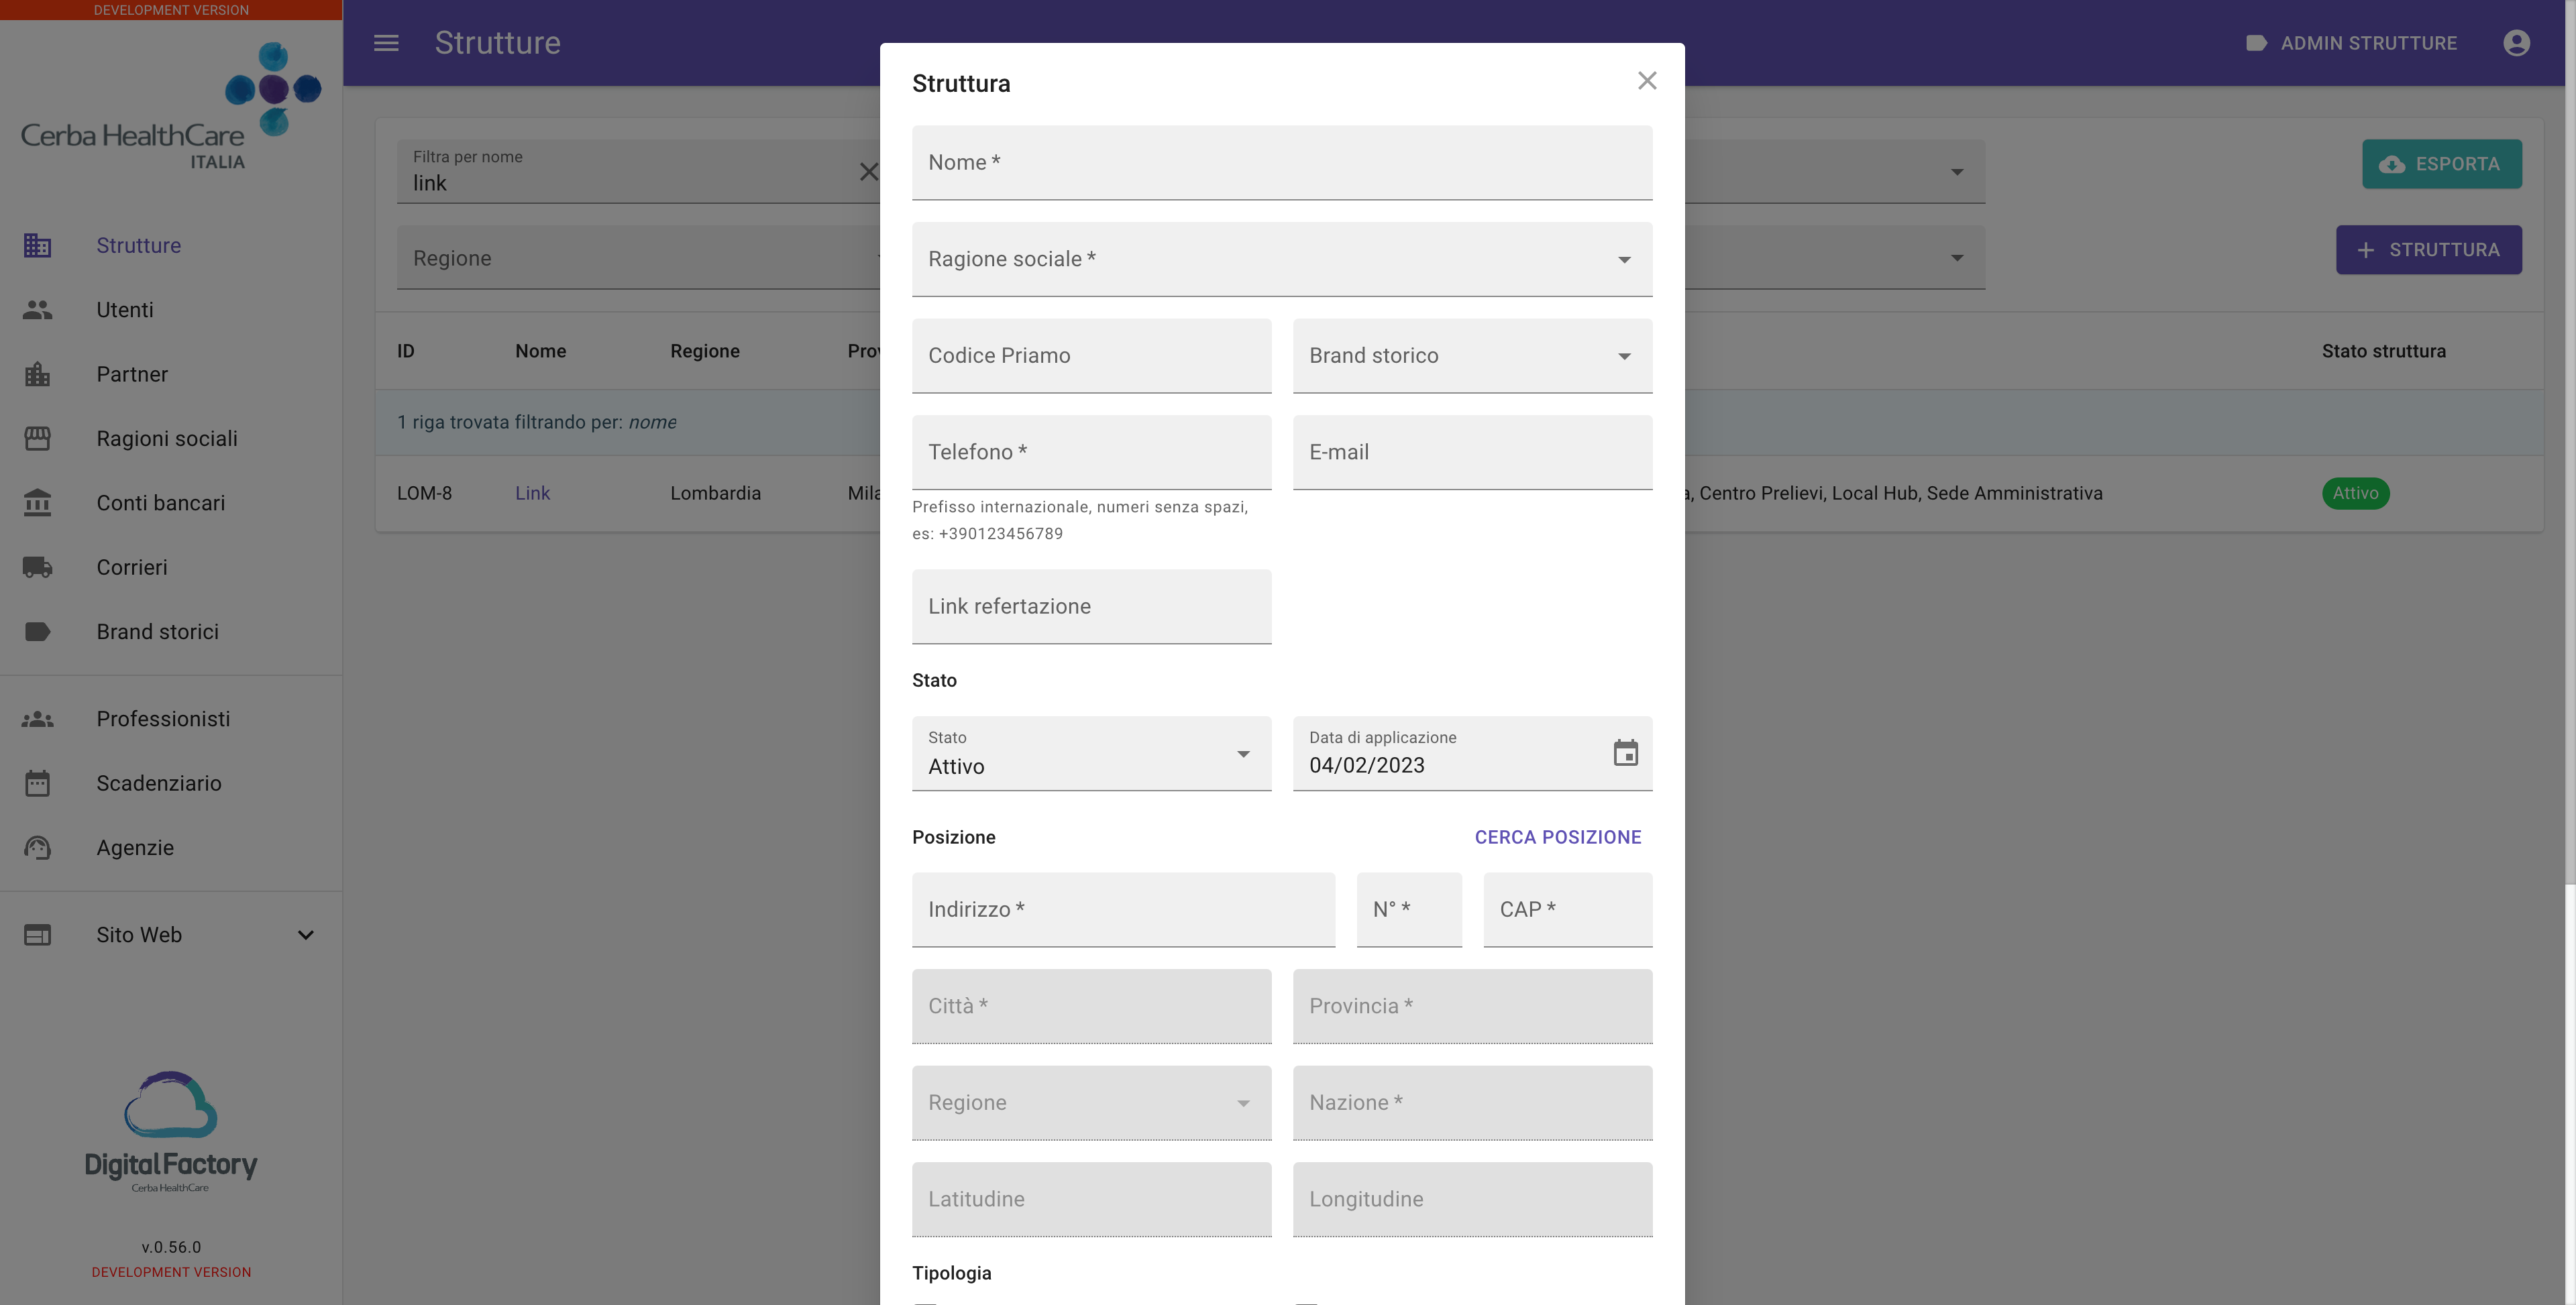
\includegraphics[width= 0.48\textwidth]{images/capitolo5/f1_f2_f3_websiteVisibility_email_links/ModalFacility_create_pt1.png}} \quad
%     \subfloat[][\emph{Modale aggiunta parte 2}]
%         {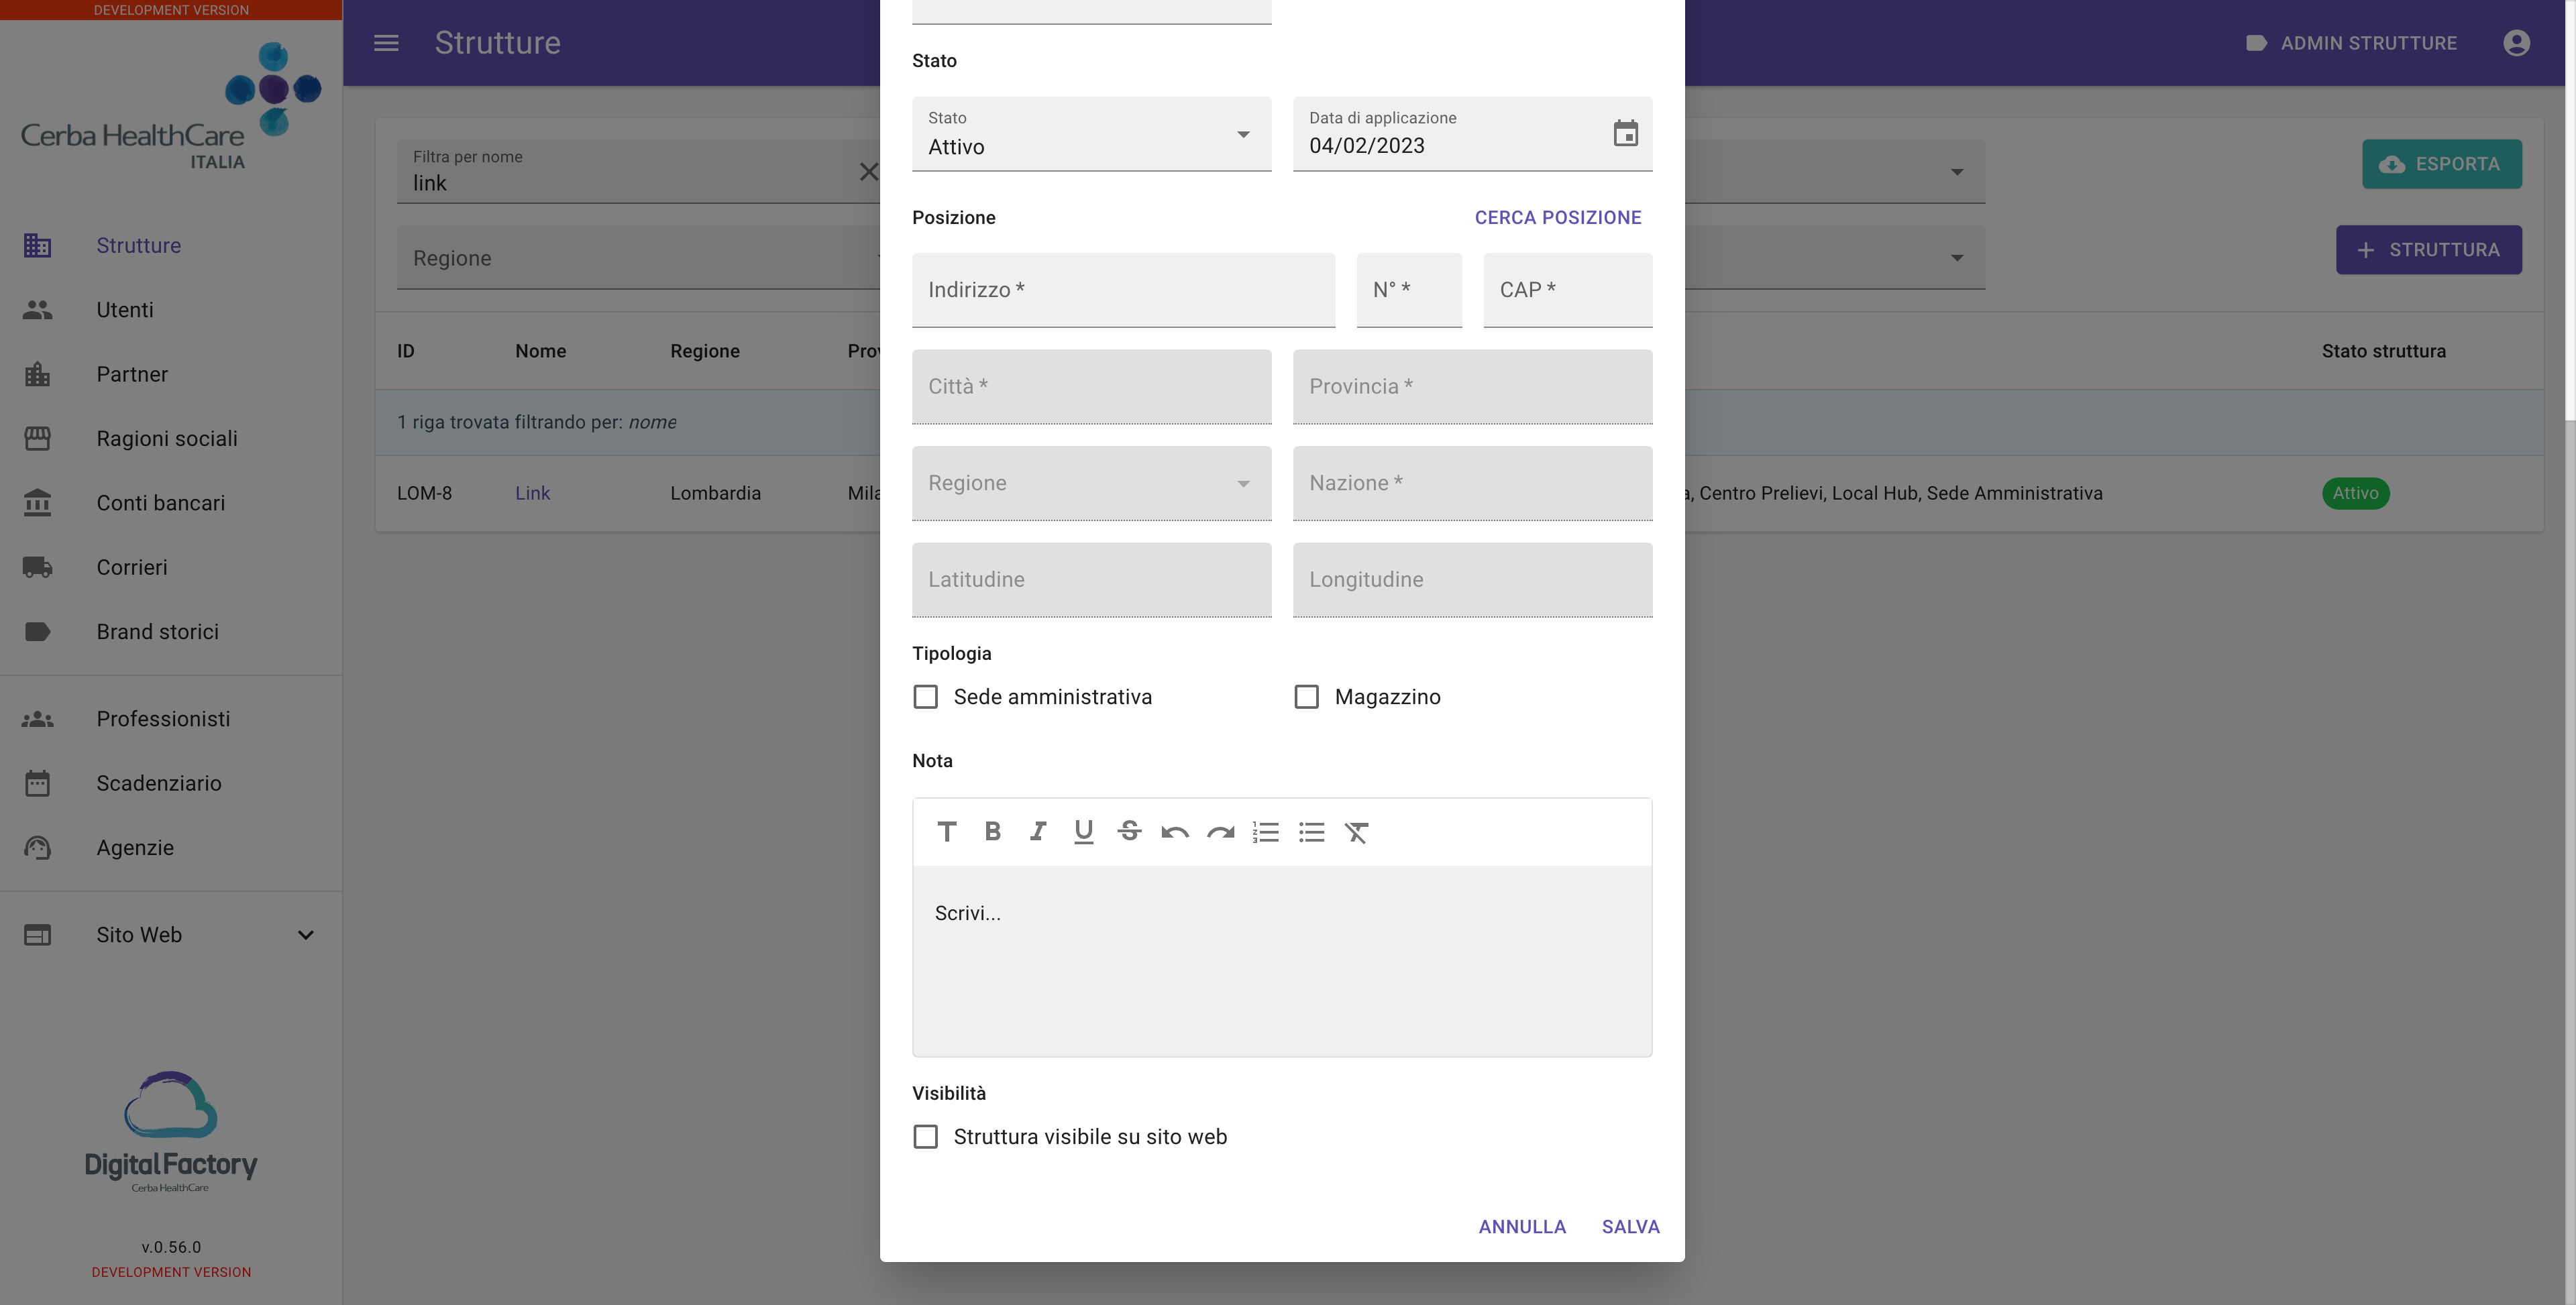
\includegraphics[width= 0.48\textwidth]{images/capitolo5/f1_f2_f3_websiteVisibility_email_links/ModalFacility_create_pt2.png}} 
%     \caption{Modale aggiunta nuova struttura}
%     % \label{fig:Modale aggiunta nuova struttura}    
% \end{figure}

% \begin{figure}[H]
%     \centering
%     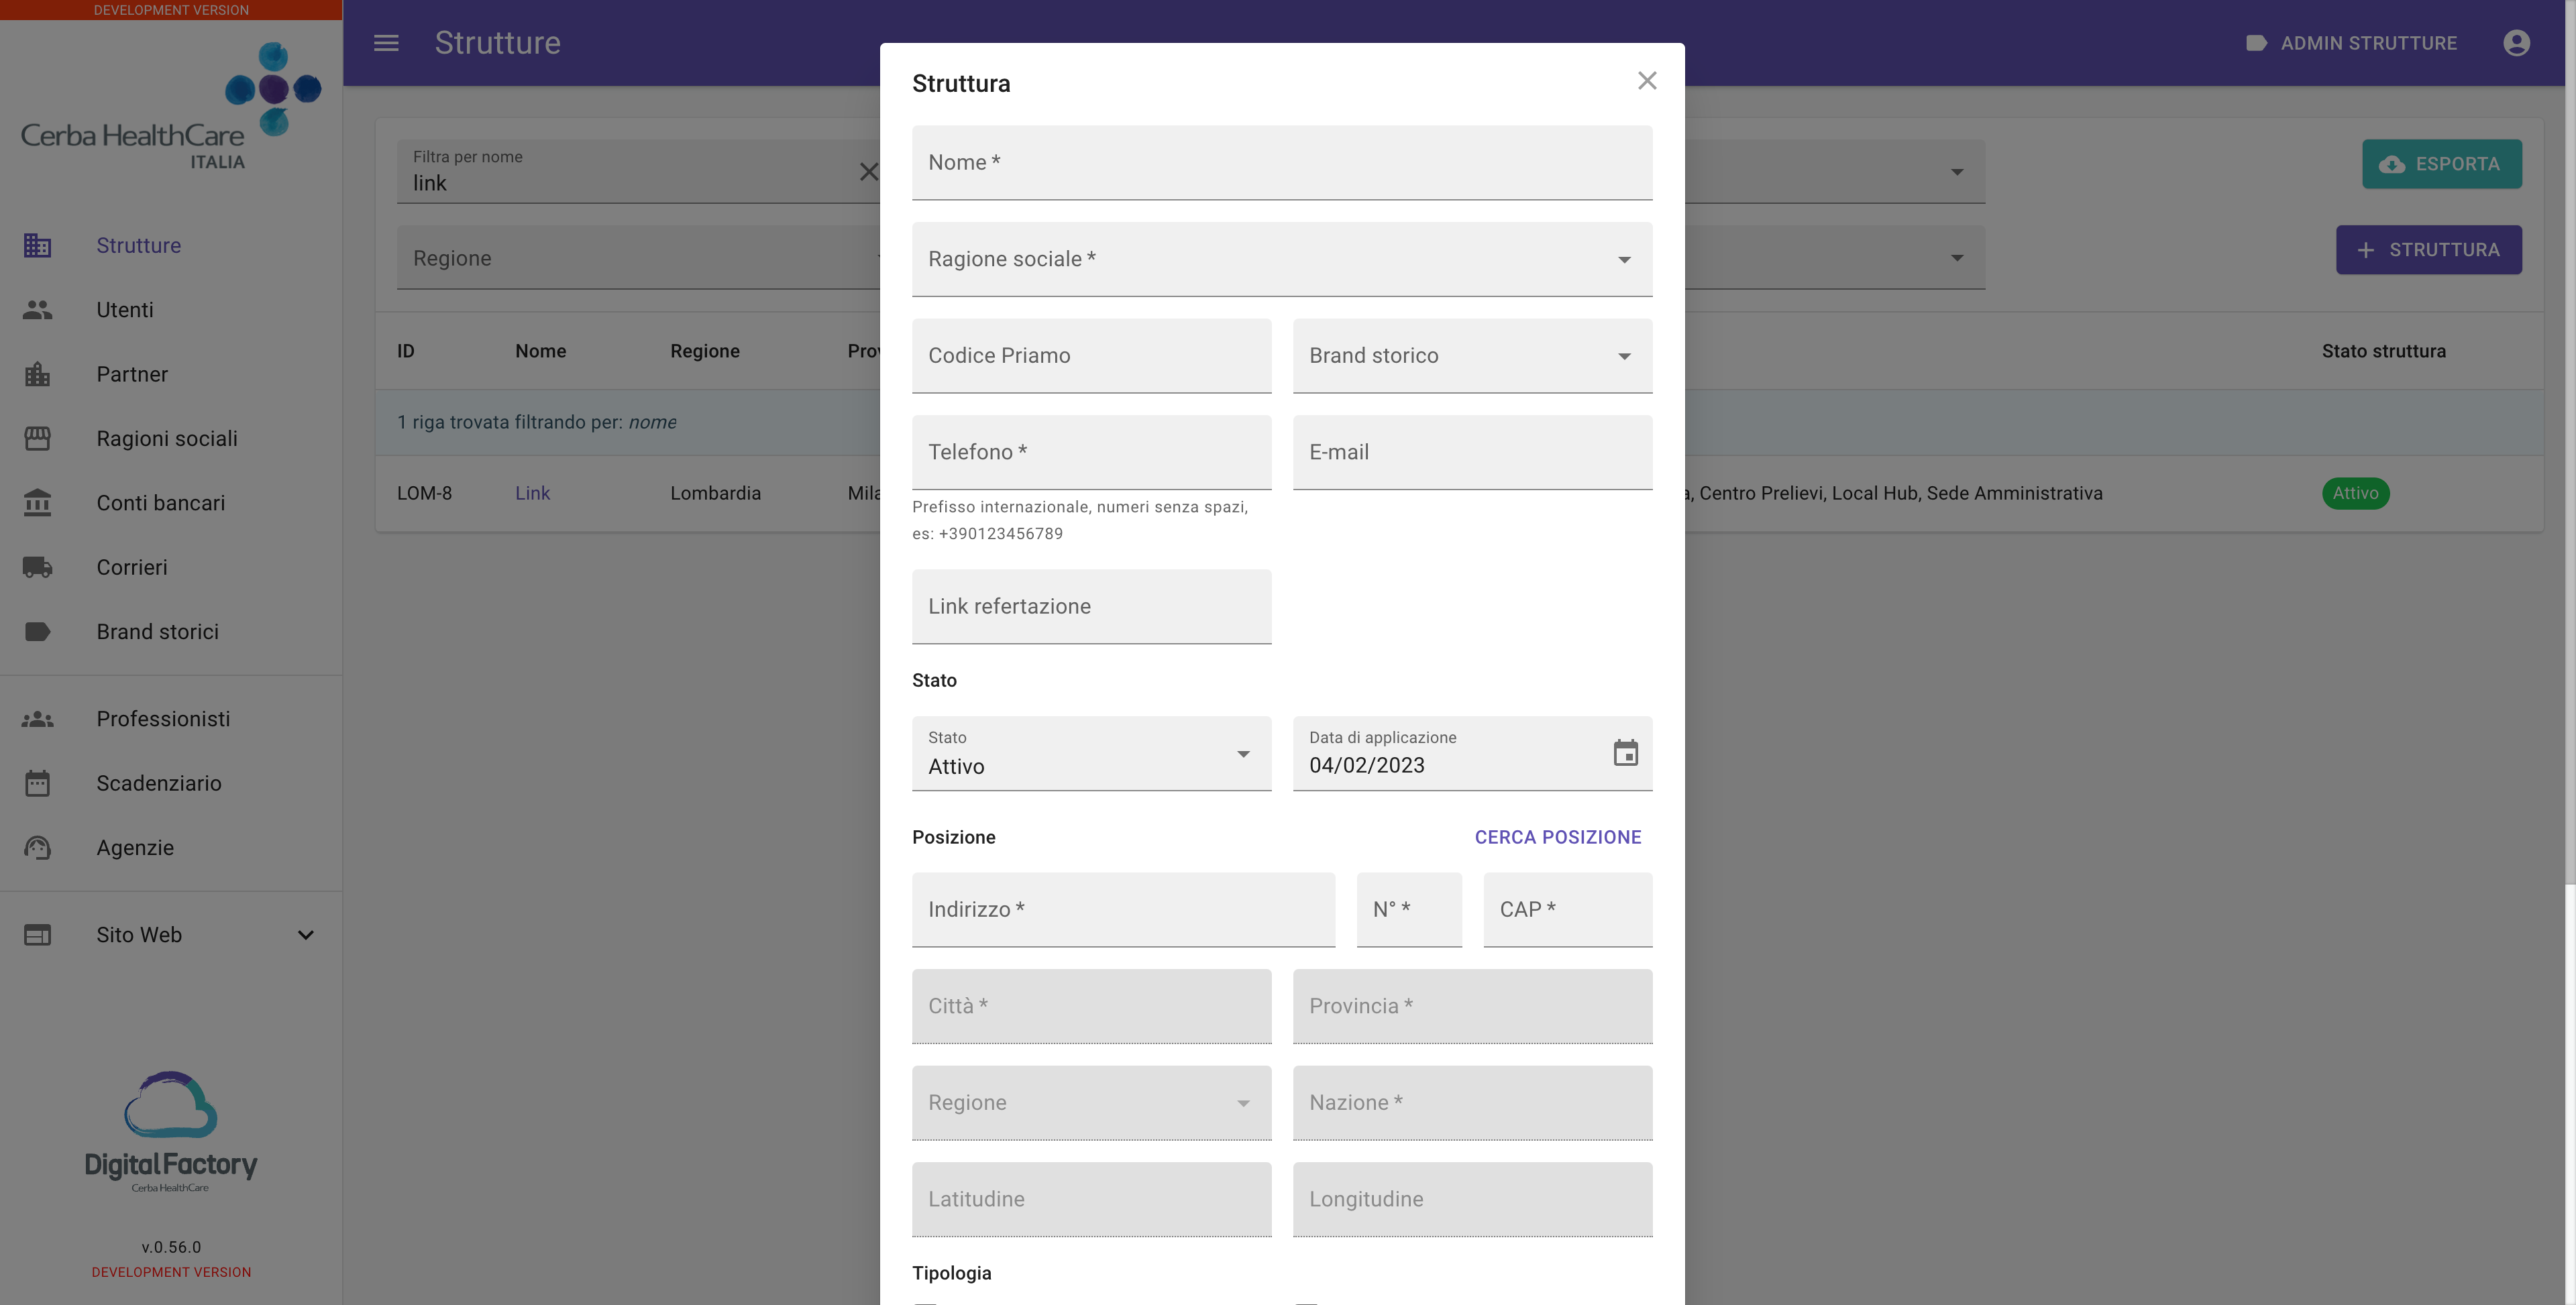
\includegraphics[width= 0.5\textwidth]{images/capitolo5/f1_f2_f3_websiteVisibility_email_links/ModalFacility_create_pt1.png} 
%     \caption{Modale aggiunta nuova struttura (pt1)} 
%     \label{fig:ModalFacility_create_pt1}
% \end{figure}

% \begin{figure}[H]
%     \centering
%     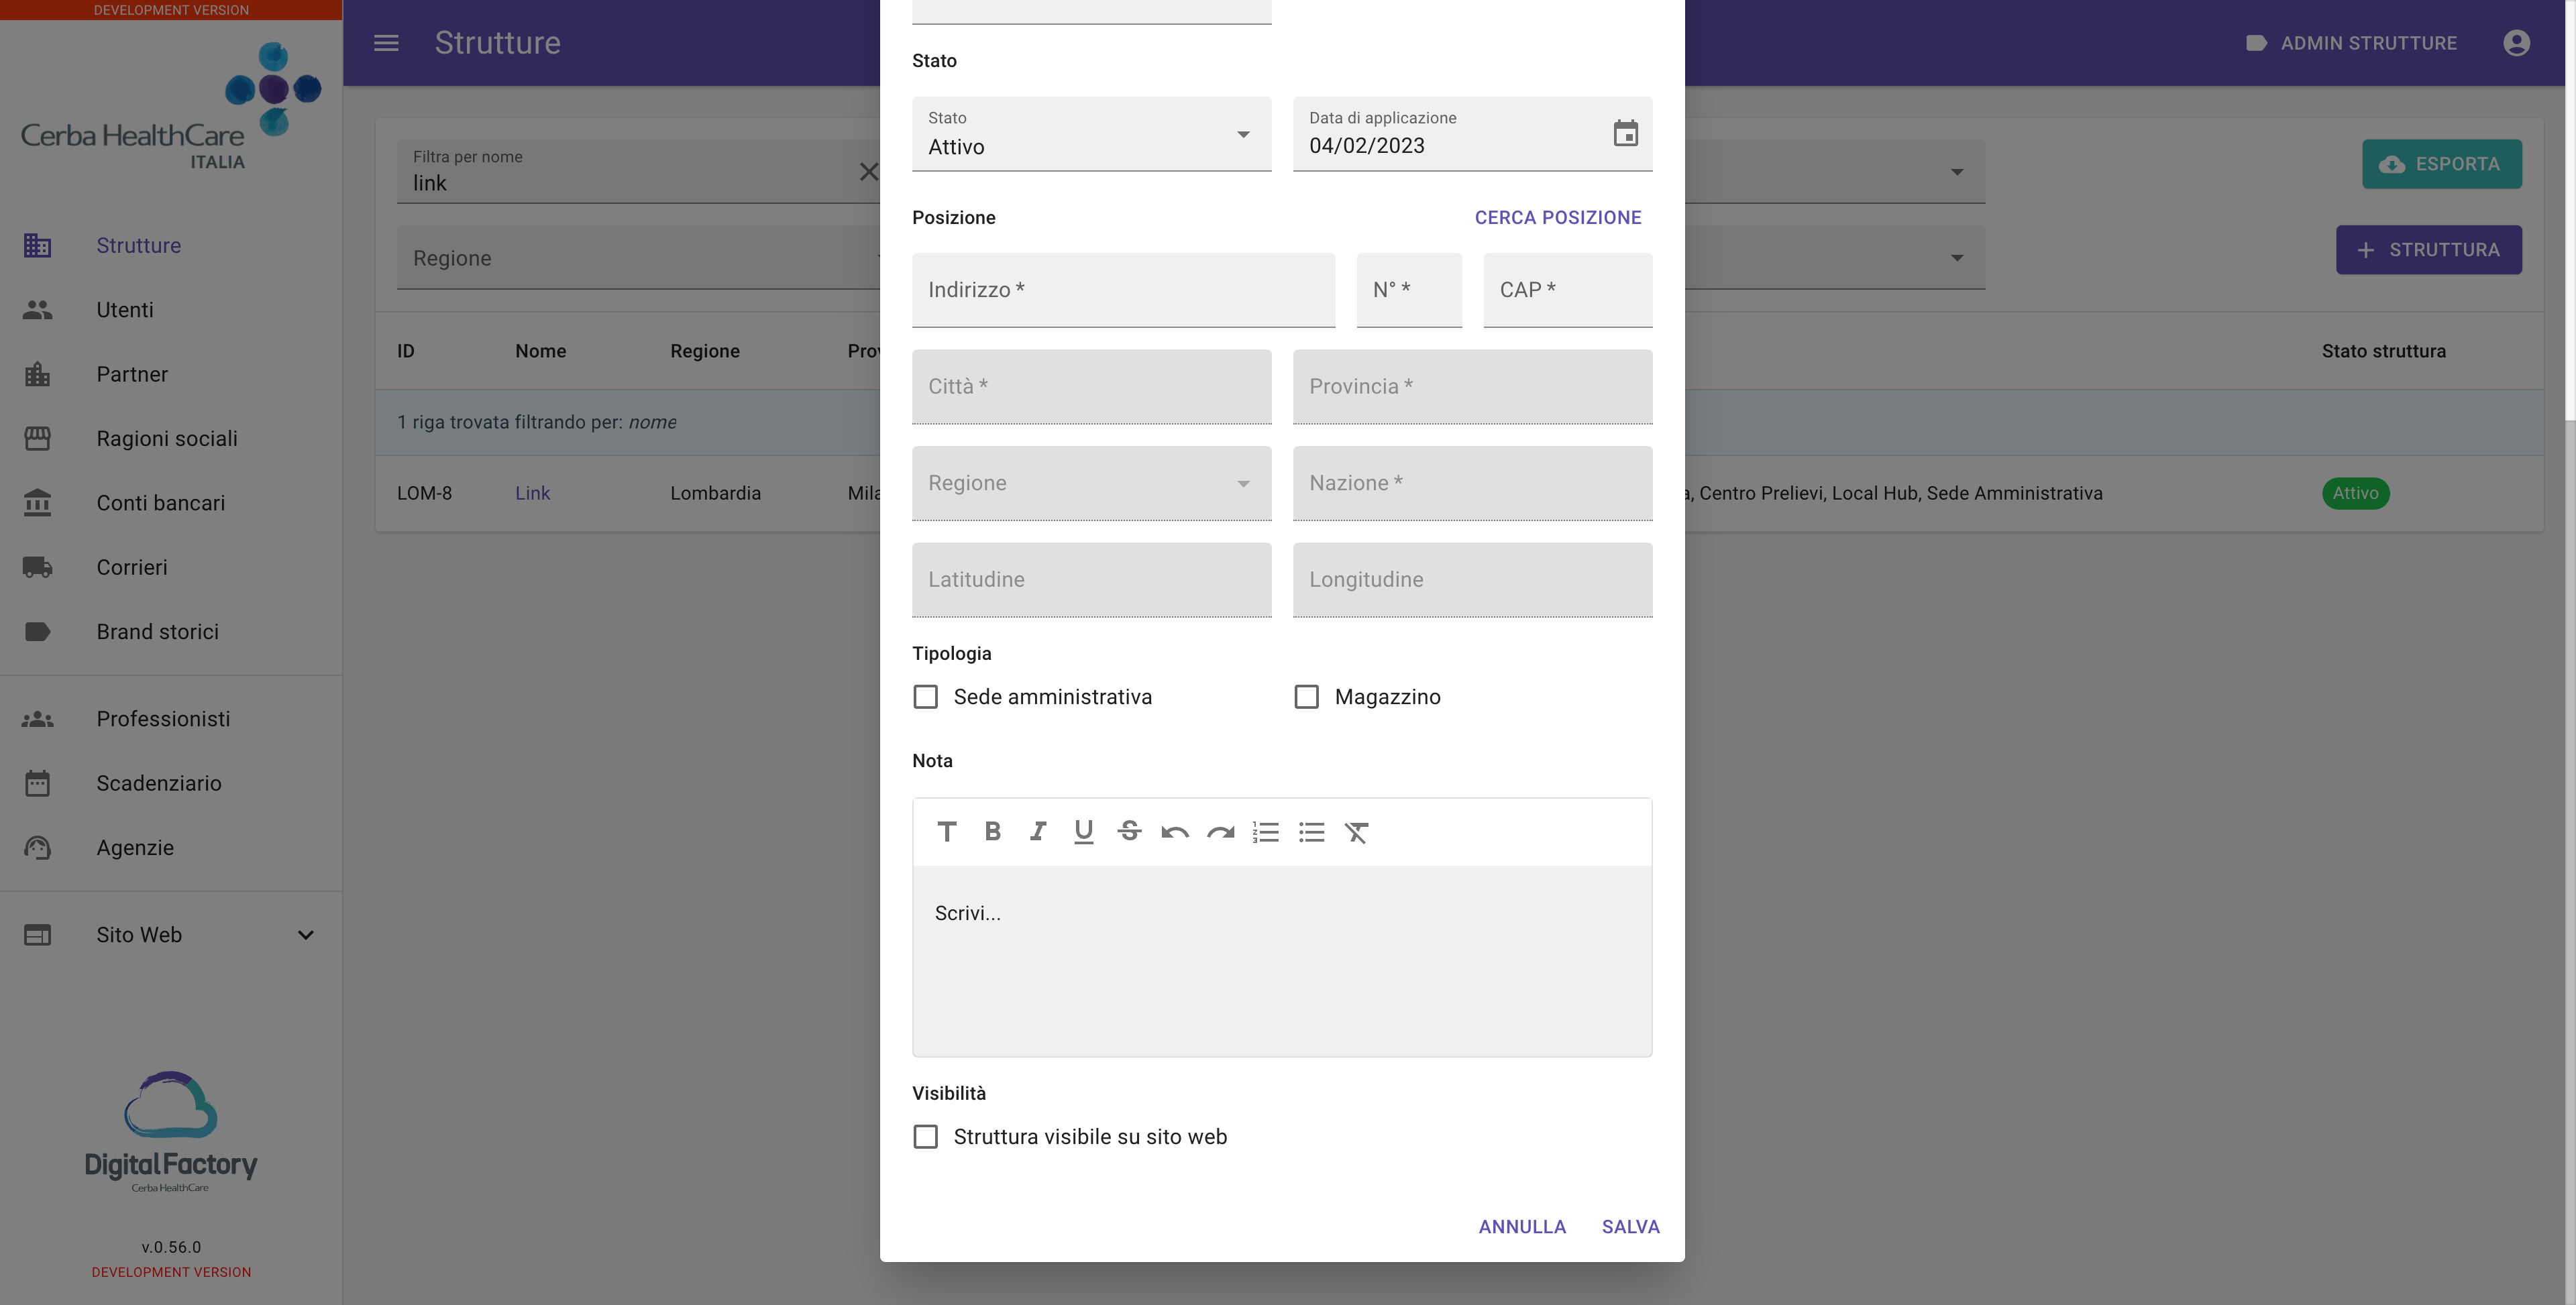
\includegraphics[width= 0.5\textwidth]{images/capitolo5/f1_f2_f3_websiteVisibility_email_links/ModalFacility_create_pt2.png} 
%     \caption{Modale aggiunta nuova struttura (pt2)} 
%     \label{fig:ModalFacility_create_pt2}
% \end{figure}

% \begin{figure}[H]
%     \centering
%     \subfloat[][\emph{Modale modifica parte 1}]
%         {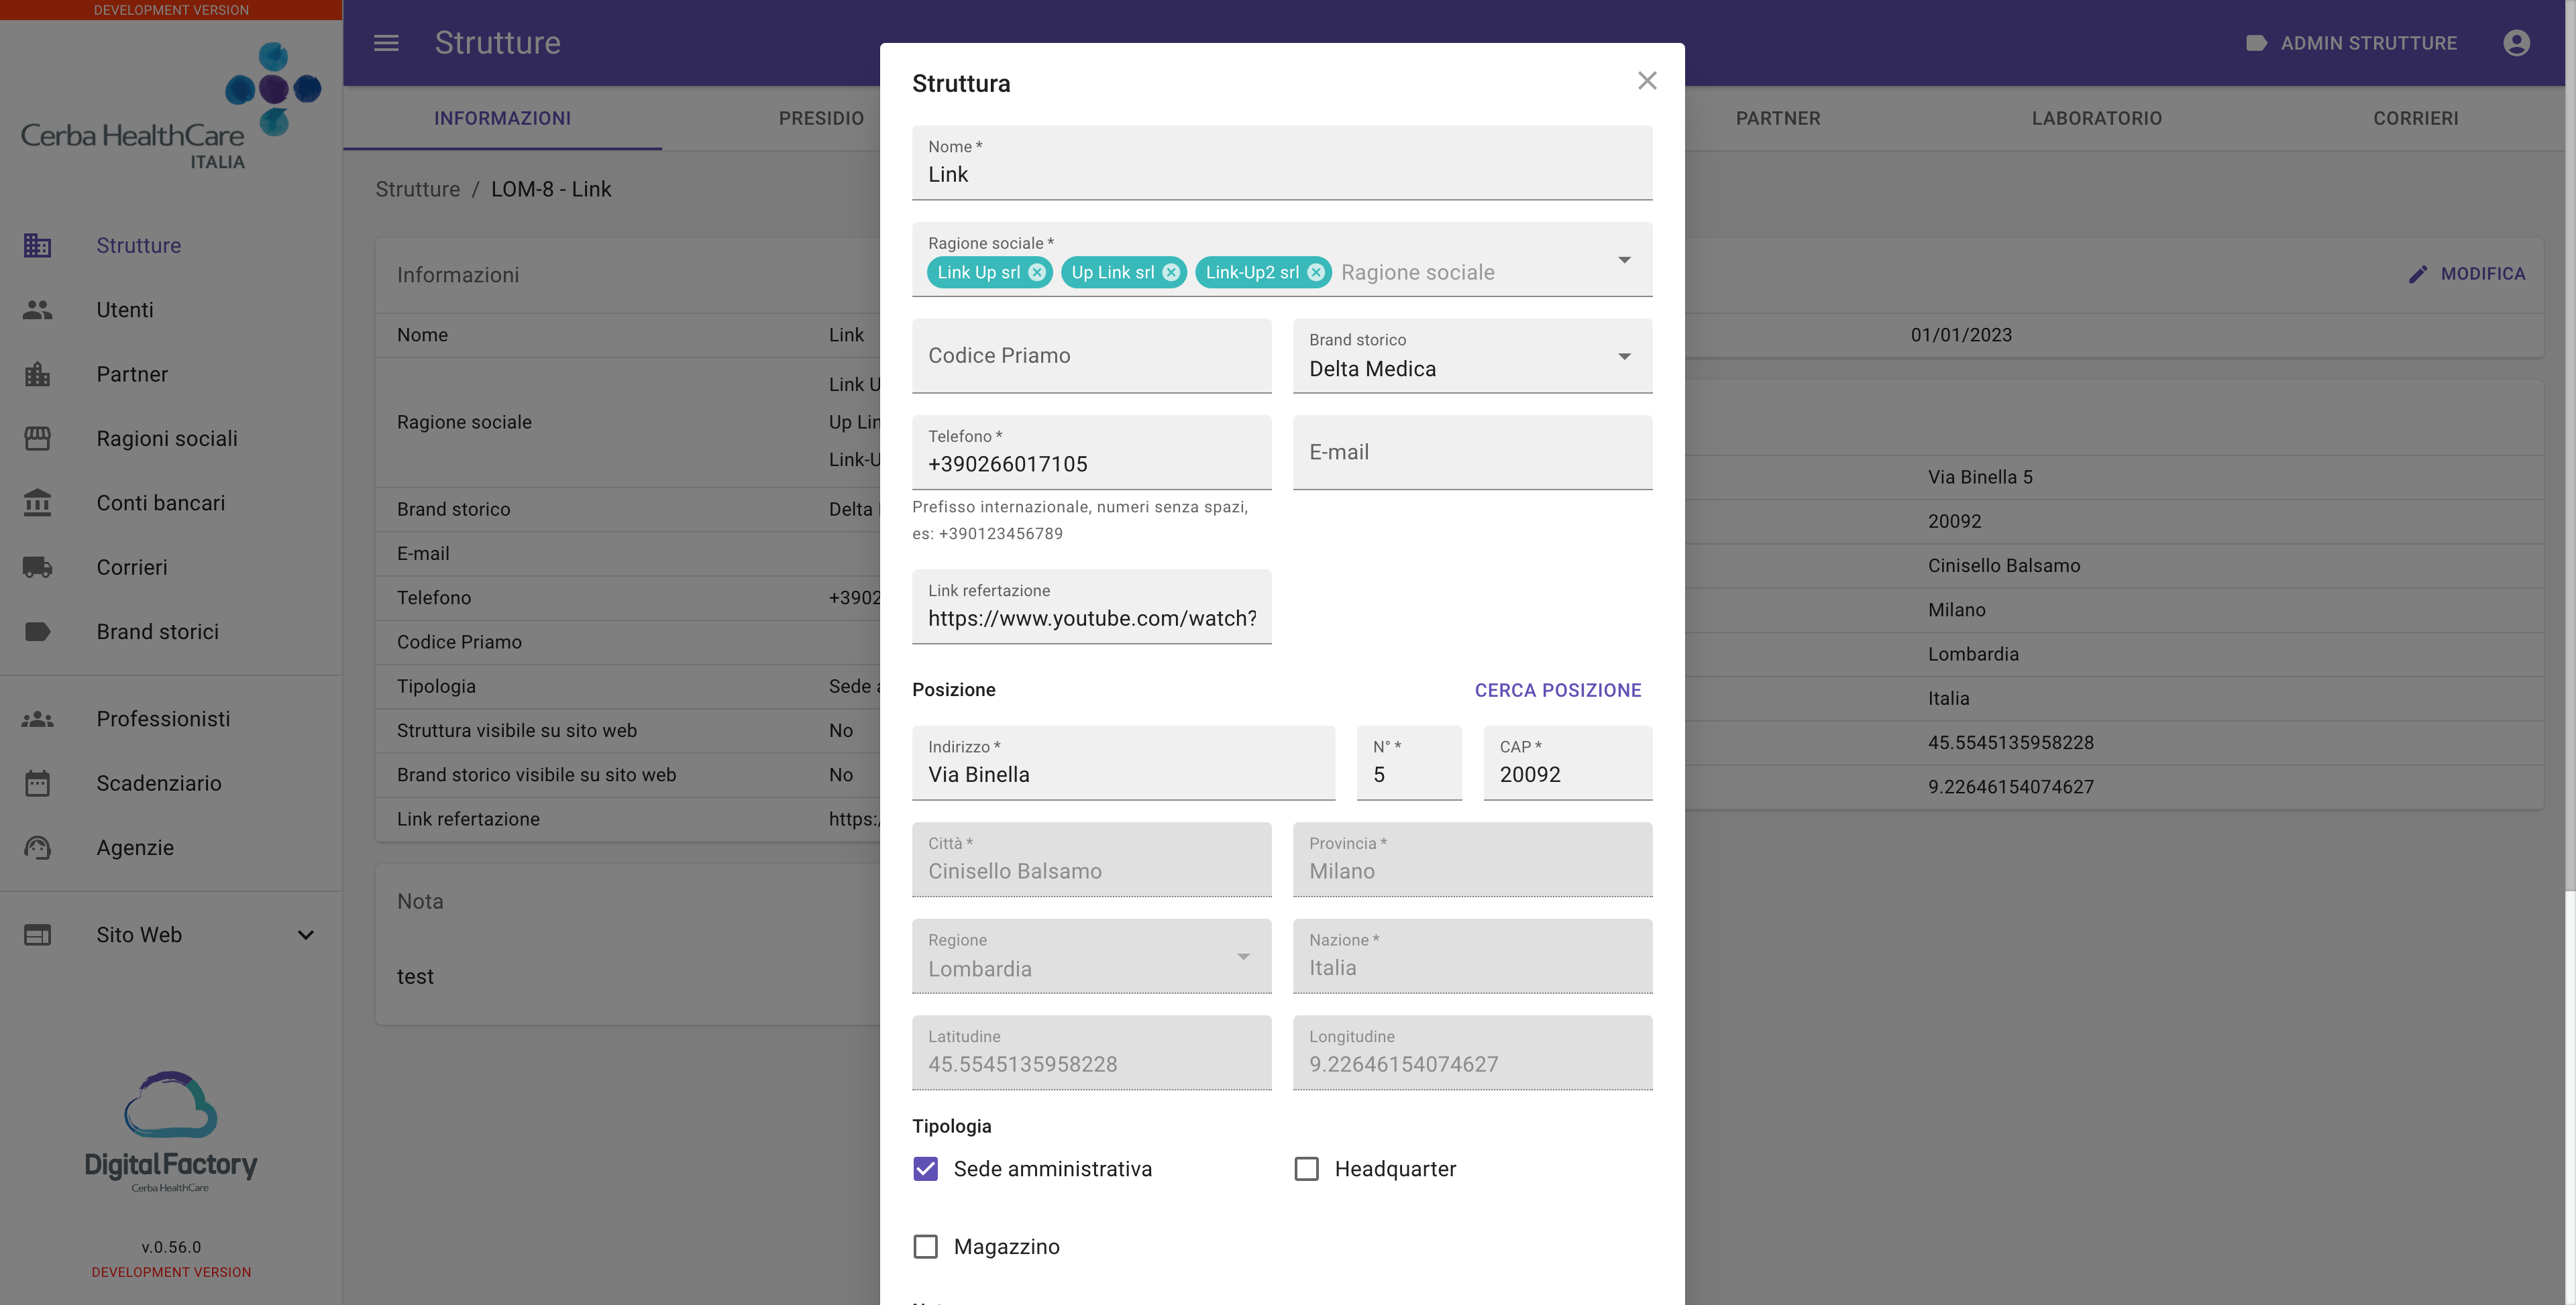
\includegraphics[width= 0.48\textwidth]{images/capitolo5/f1_f2_f3_websiteVisibility_email_links/ModalFacility_edit_pt1.png}} \quad
%     \subfloat[][\emph{Modale modifica parte 2}]
%         {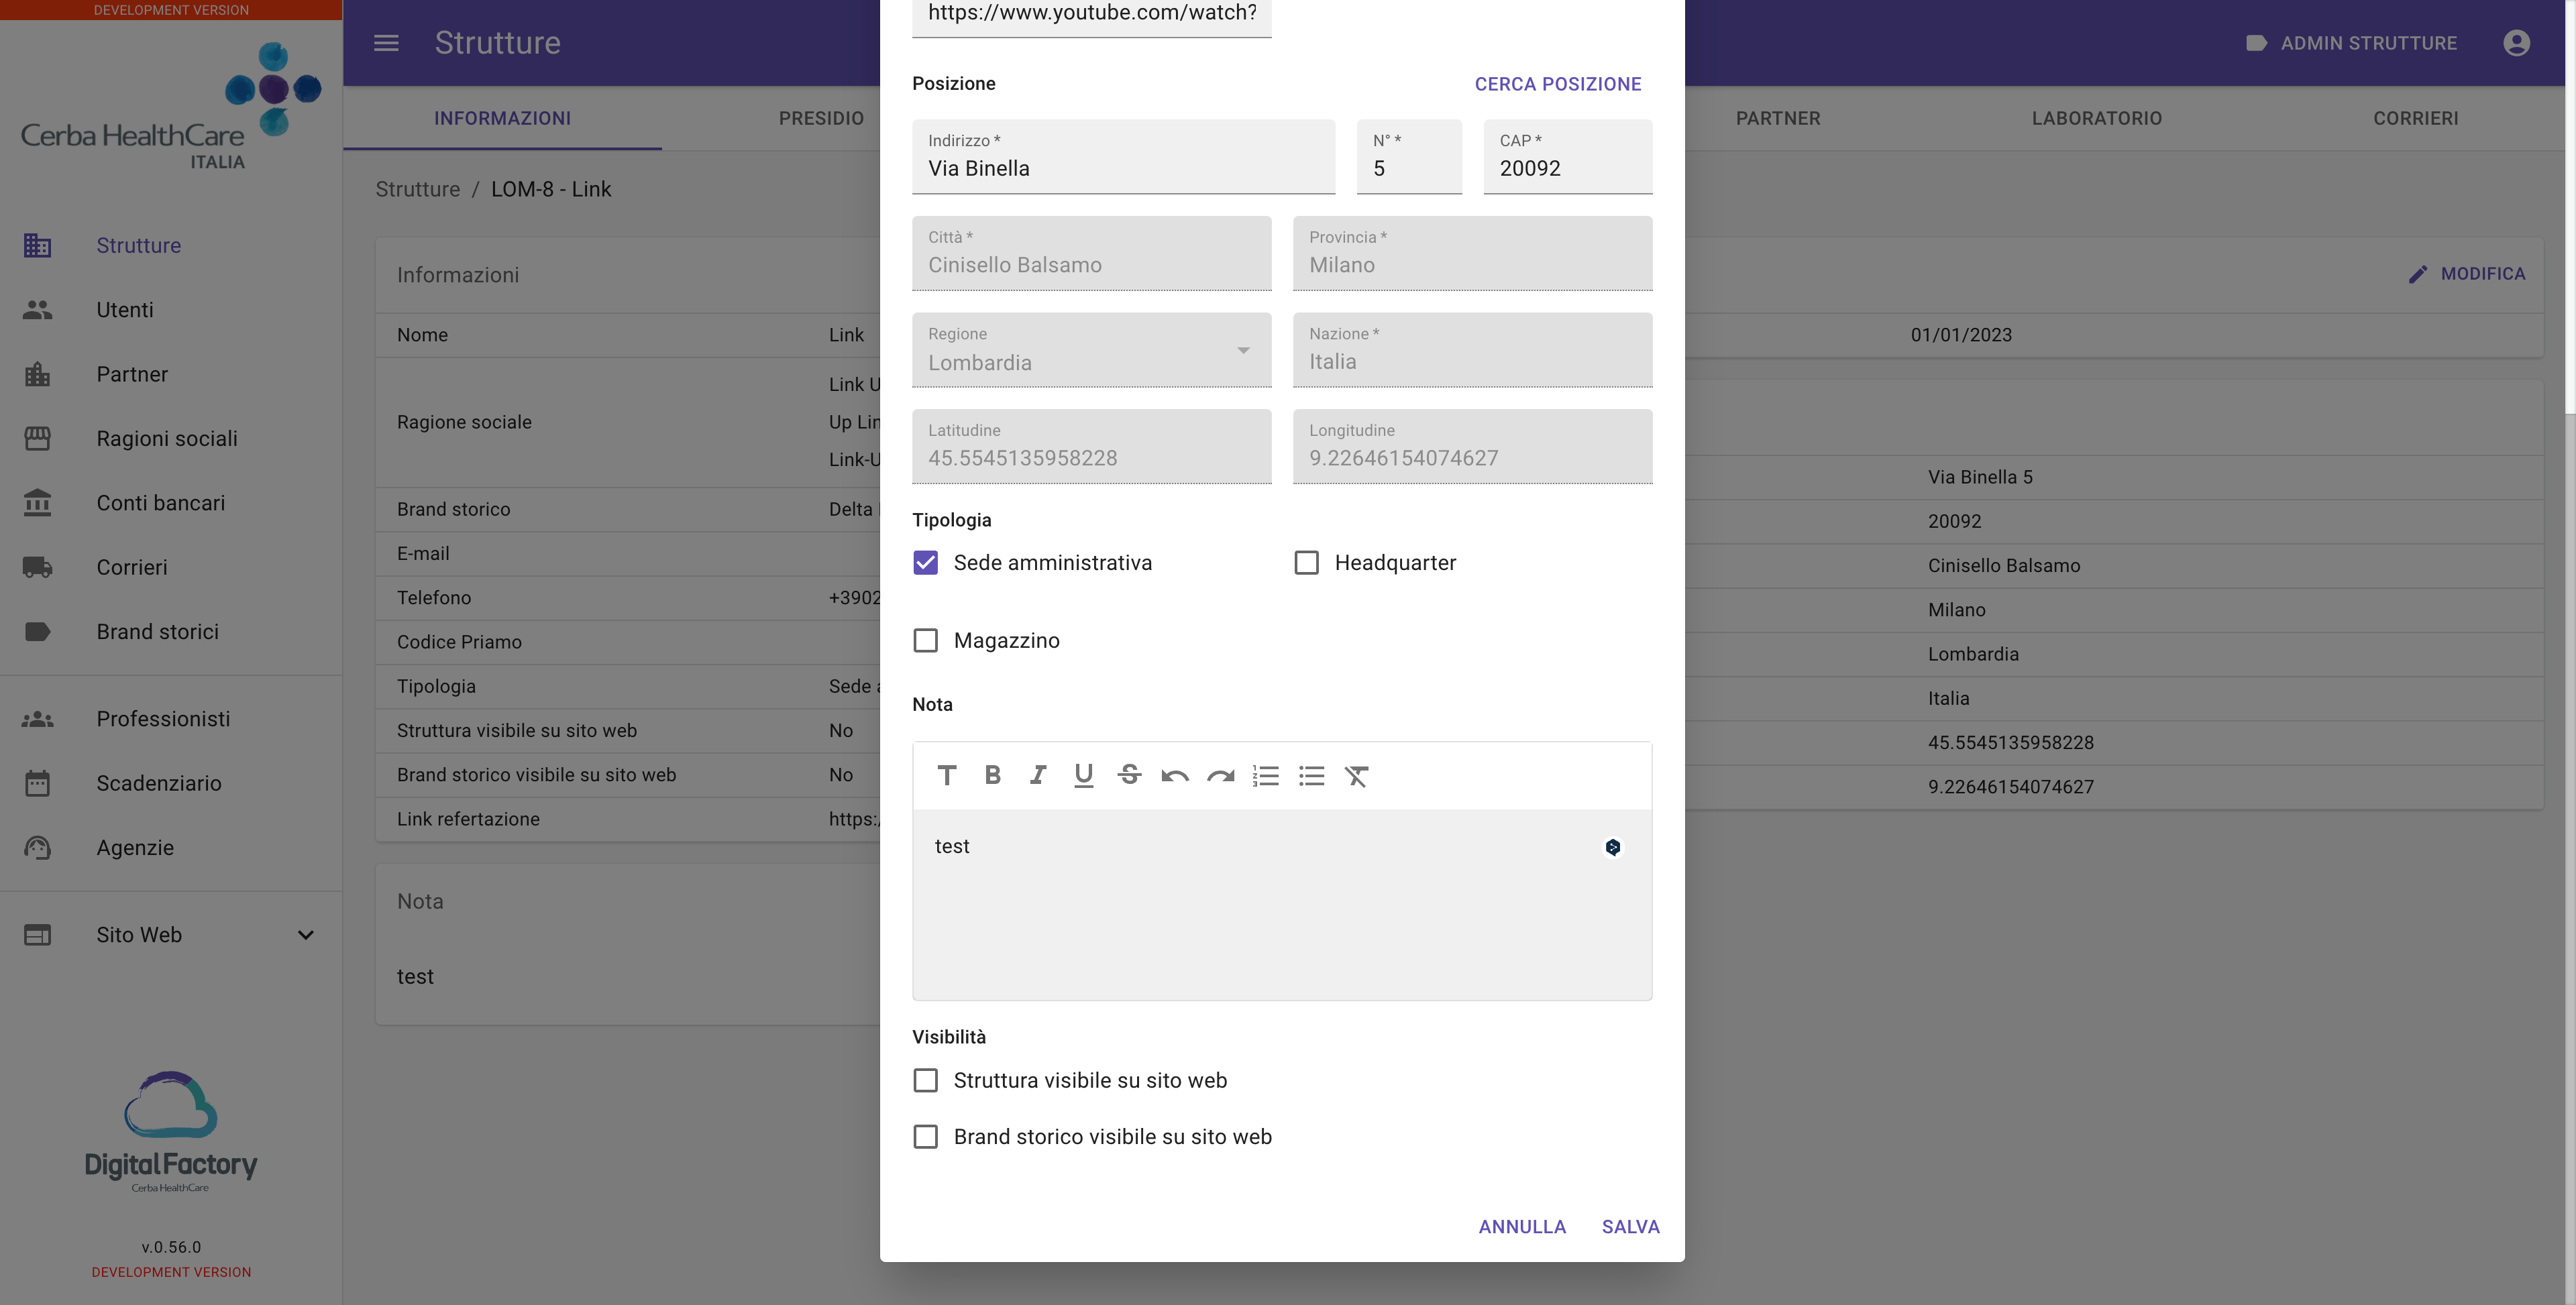
\includegraphics[width= 0.48\textwidth]{images/capitolo5/f1_f2_f3_websiteVisibility_email_links/ModalFacility_edit_pt2.png}} 
%     \caption{Modale modifica struttura esistente}
%     % \label{fig:Modale modifica struttura esistente}    
% \end{figure}

% \begin{figure}[H]
%     \centering
%     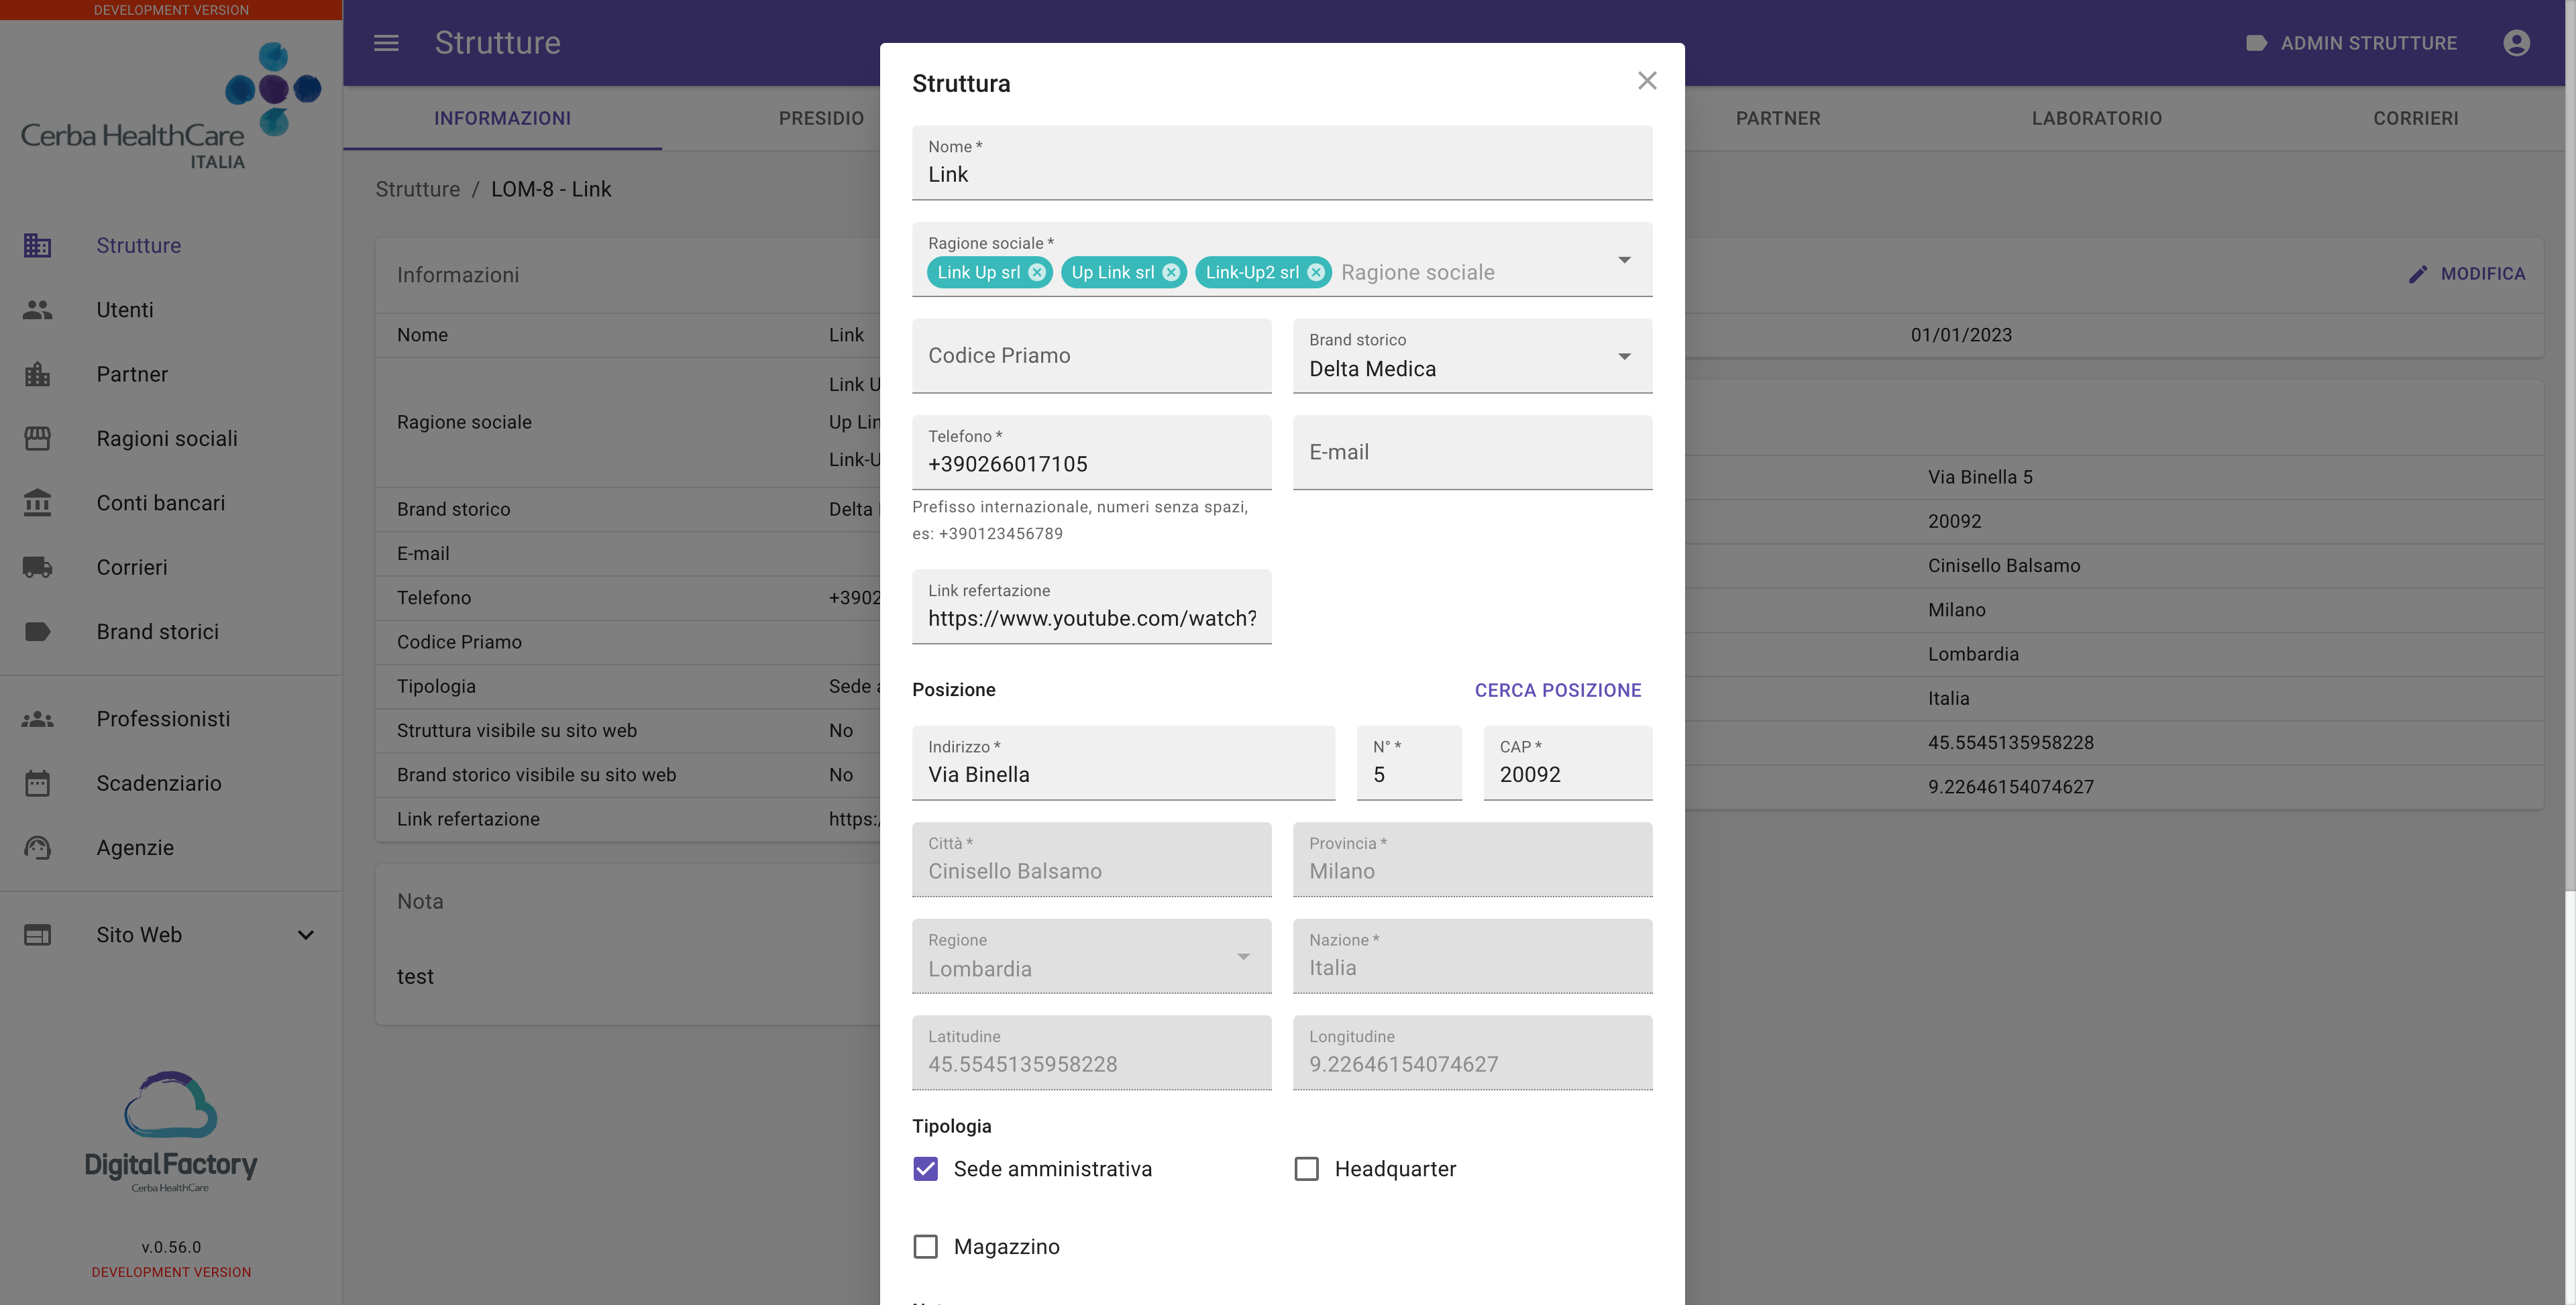
\includegraphics[width= 0.5\textwidth]{images/capitolo5/f1_f2_f3_websiteVisibility_email_links/ModalFacility_edit_pt1.png} 
%     \caption{Modale modifica struttura esistente (pt1)} 
%     \label{fig:ModalFacility_edit_pt1}
% \end{figure}

% \begin{figure}[H]
%     \centering
%     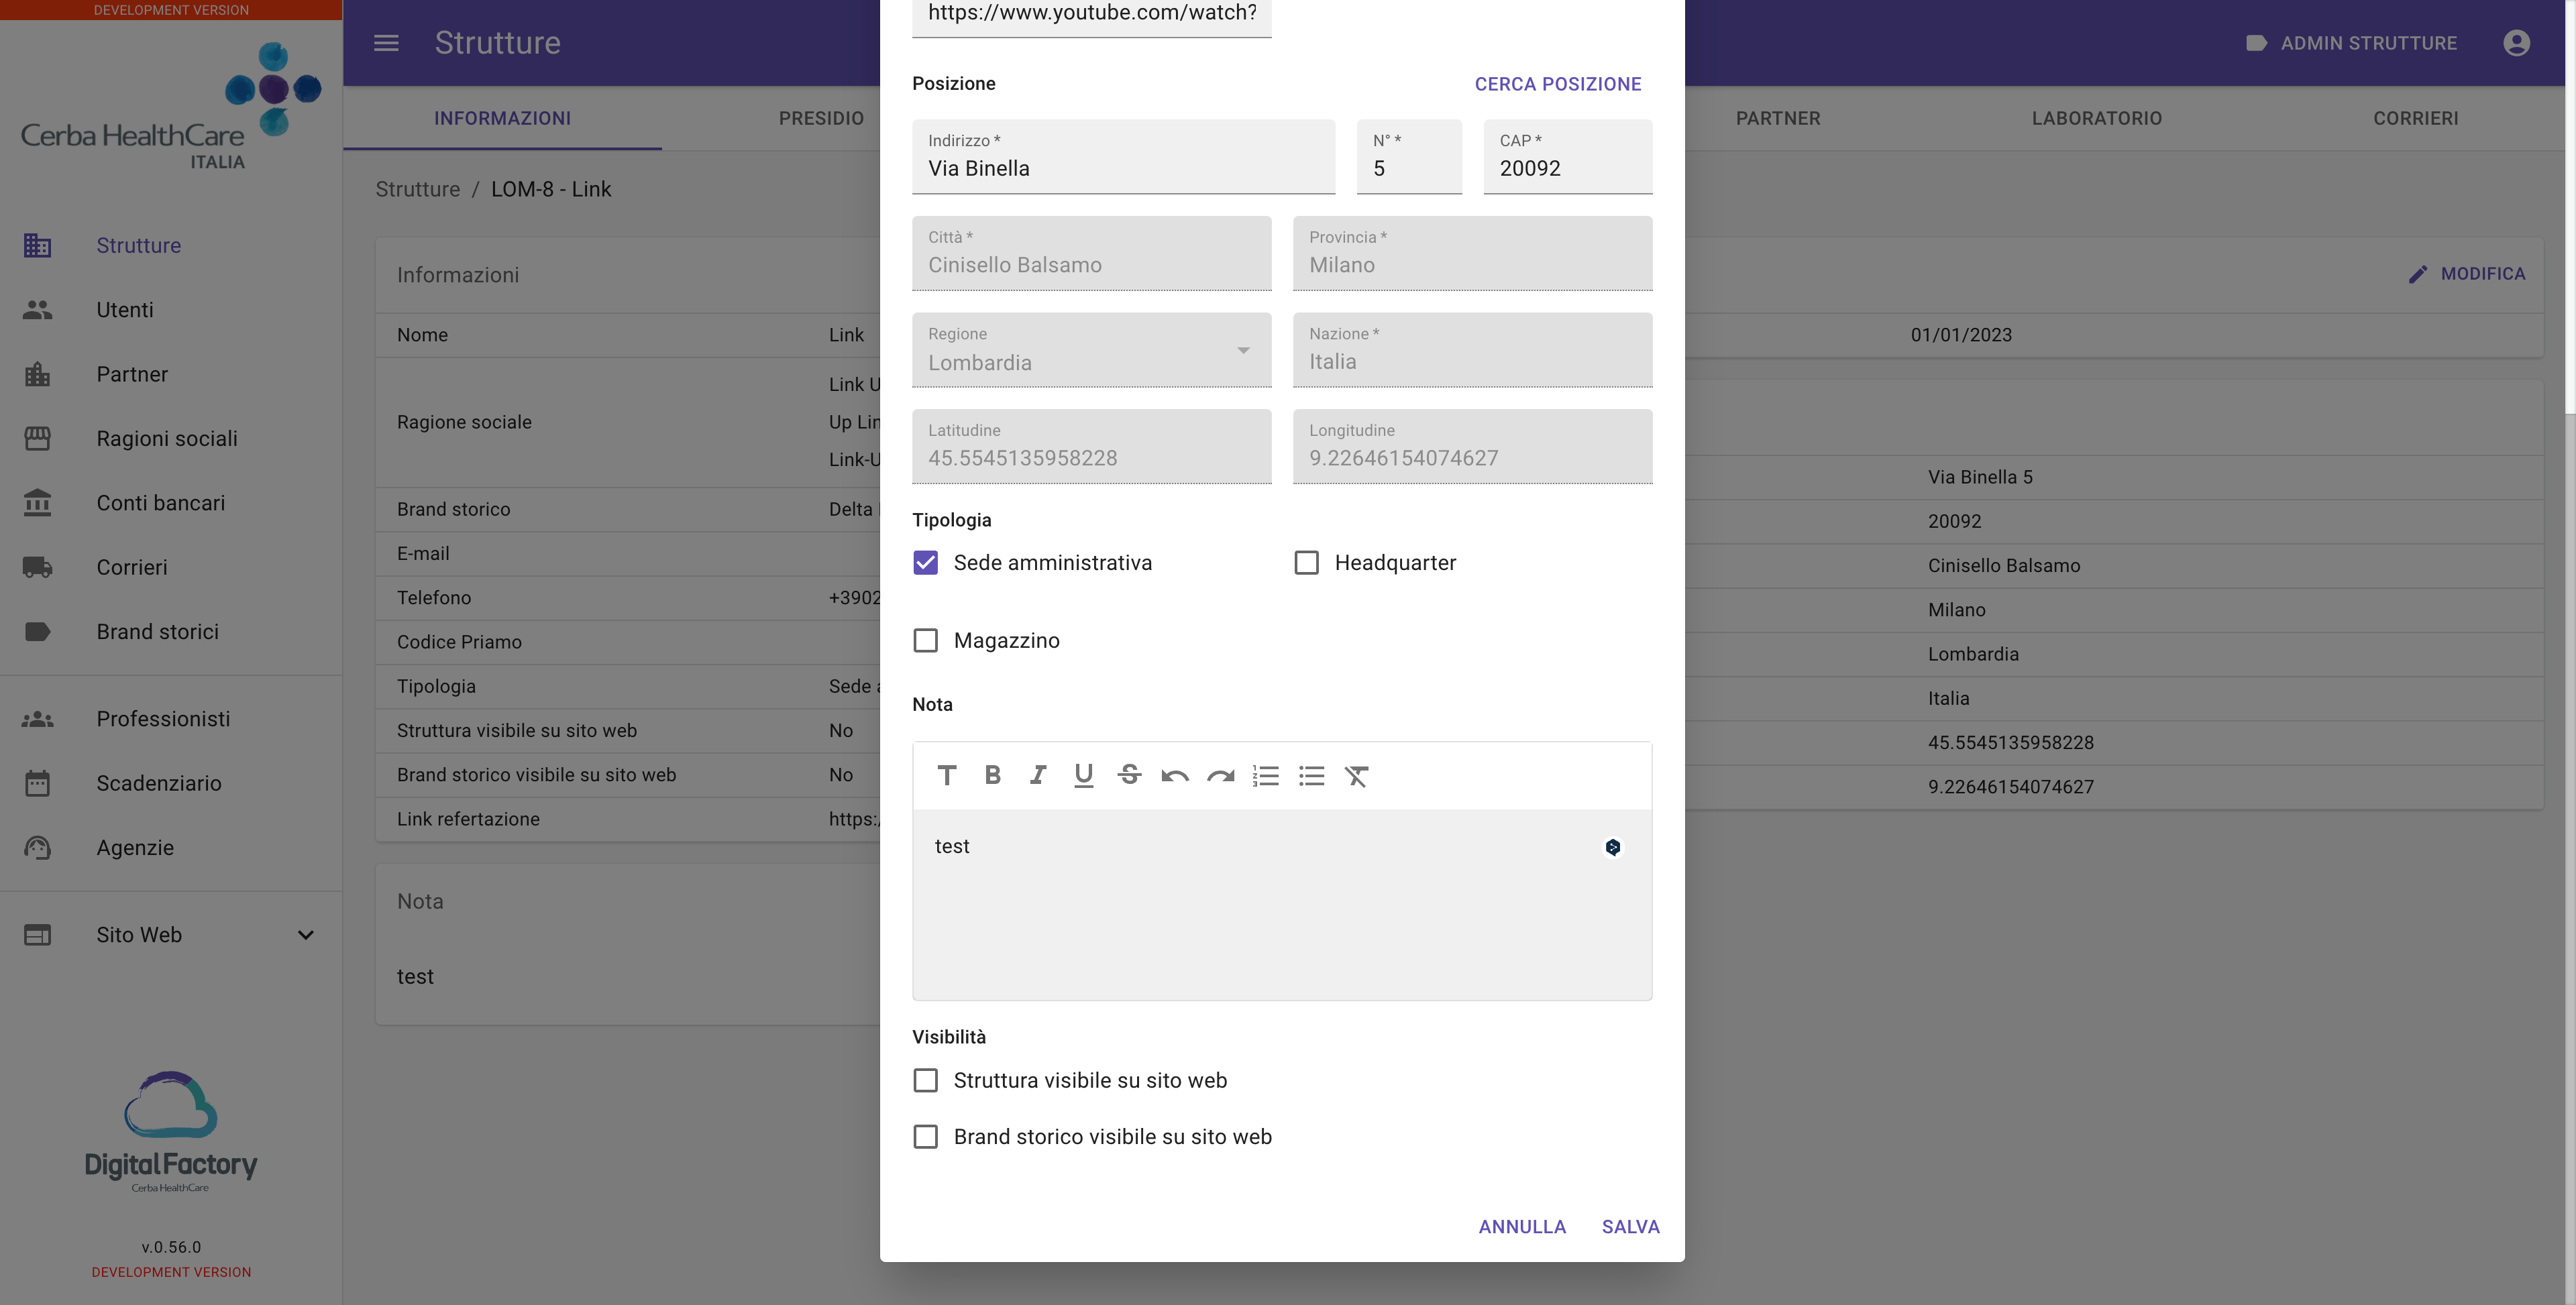
\includegraphics[width= 0.5\textwidth]{images/capitolo5/f1_f2_f3_websiteVisibility_email_links/ModalFacility_edit_pt2.png} 
%     \caption{Modale modifica struttura esistente (pt2)} 
%     \label{fig:ModalFacility_edit_pt2}
% \end{figure}

\begin{figure}[H]
    \centering
    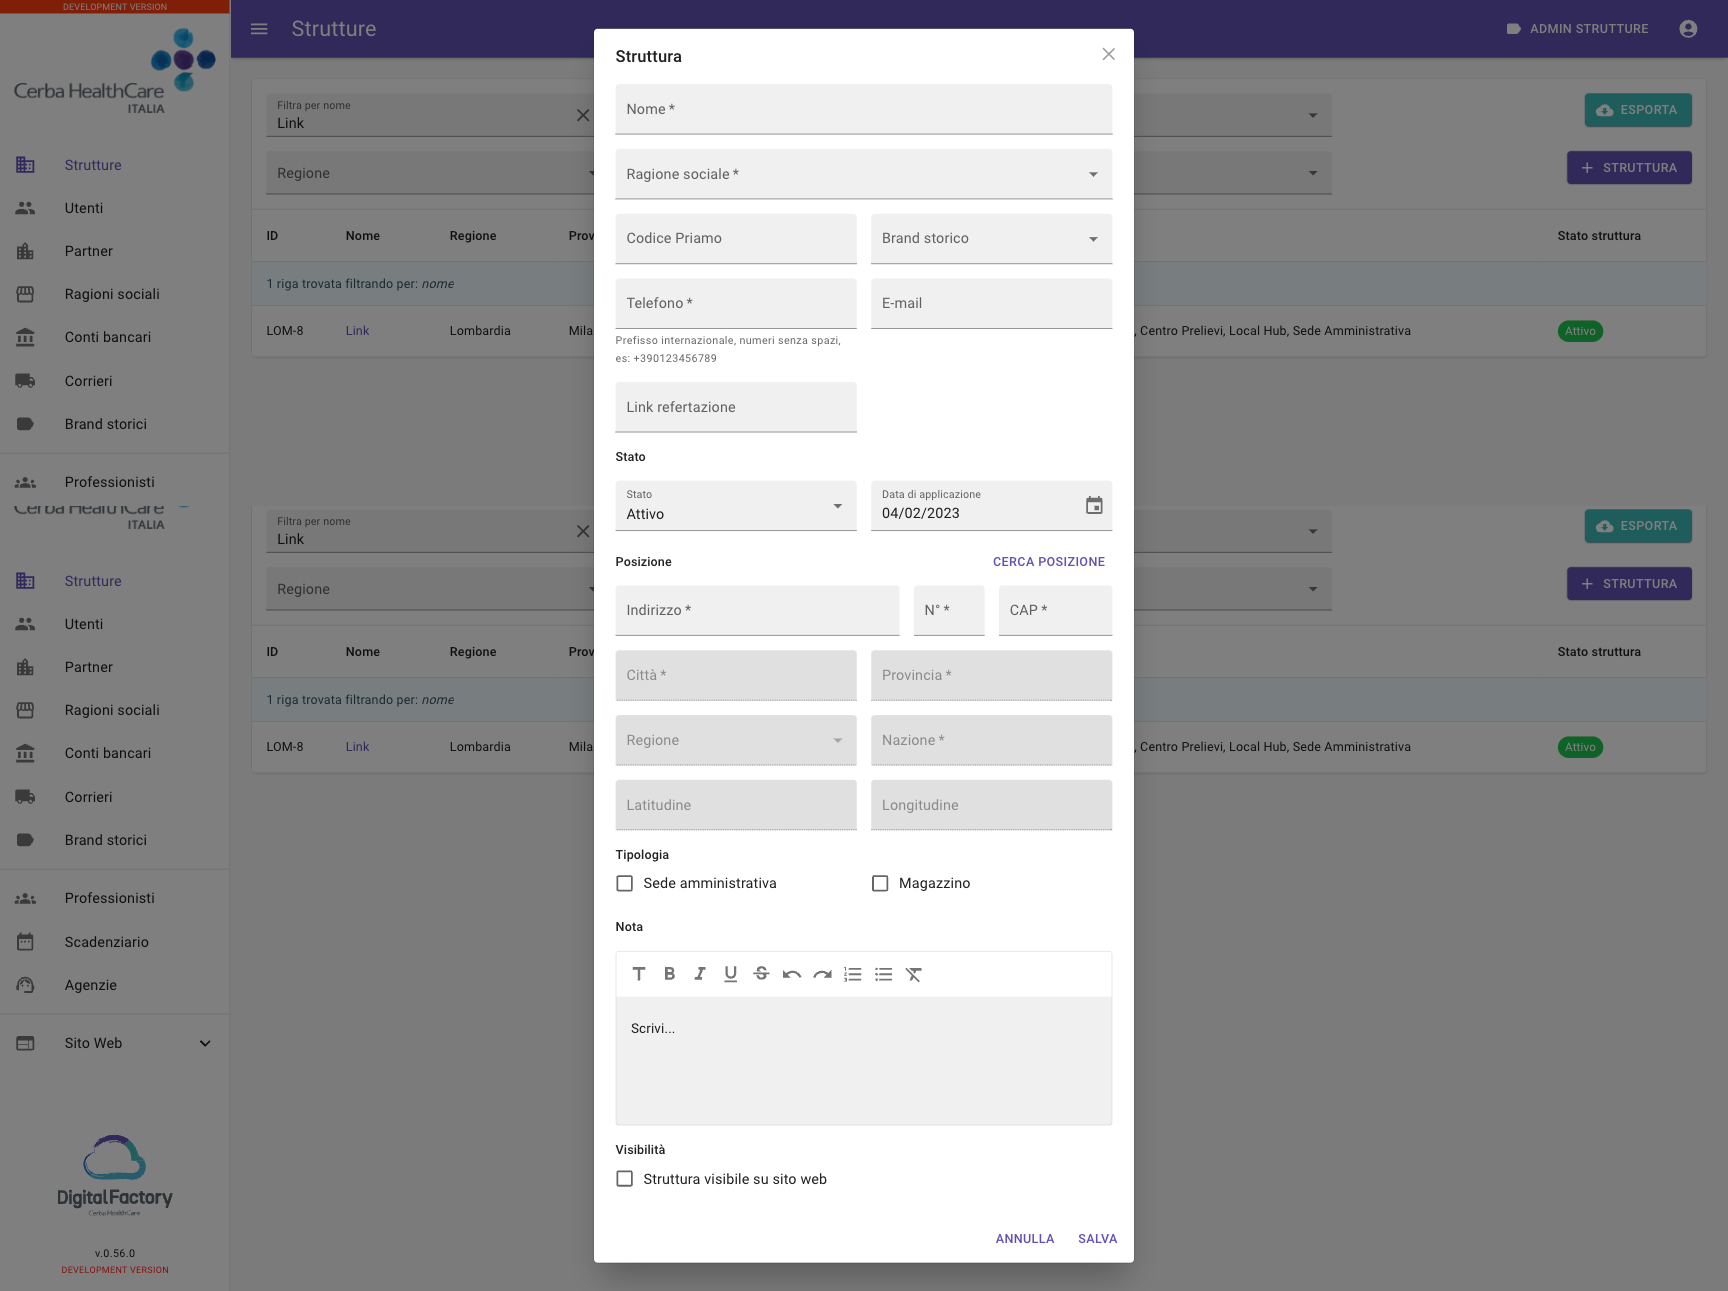
\includegraphics[width= 0.7\textwidth]{images/capitolo5/f1_f2_f3_websiteVisibility_email_links/ModalFacility_create.png} 
    \caption{Modale aggiunta nuova struttura} 
    \label{fig:ModalFacility_create}
\end{figure}

\begin{figure}[H]
    \centering
    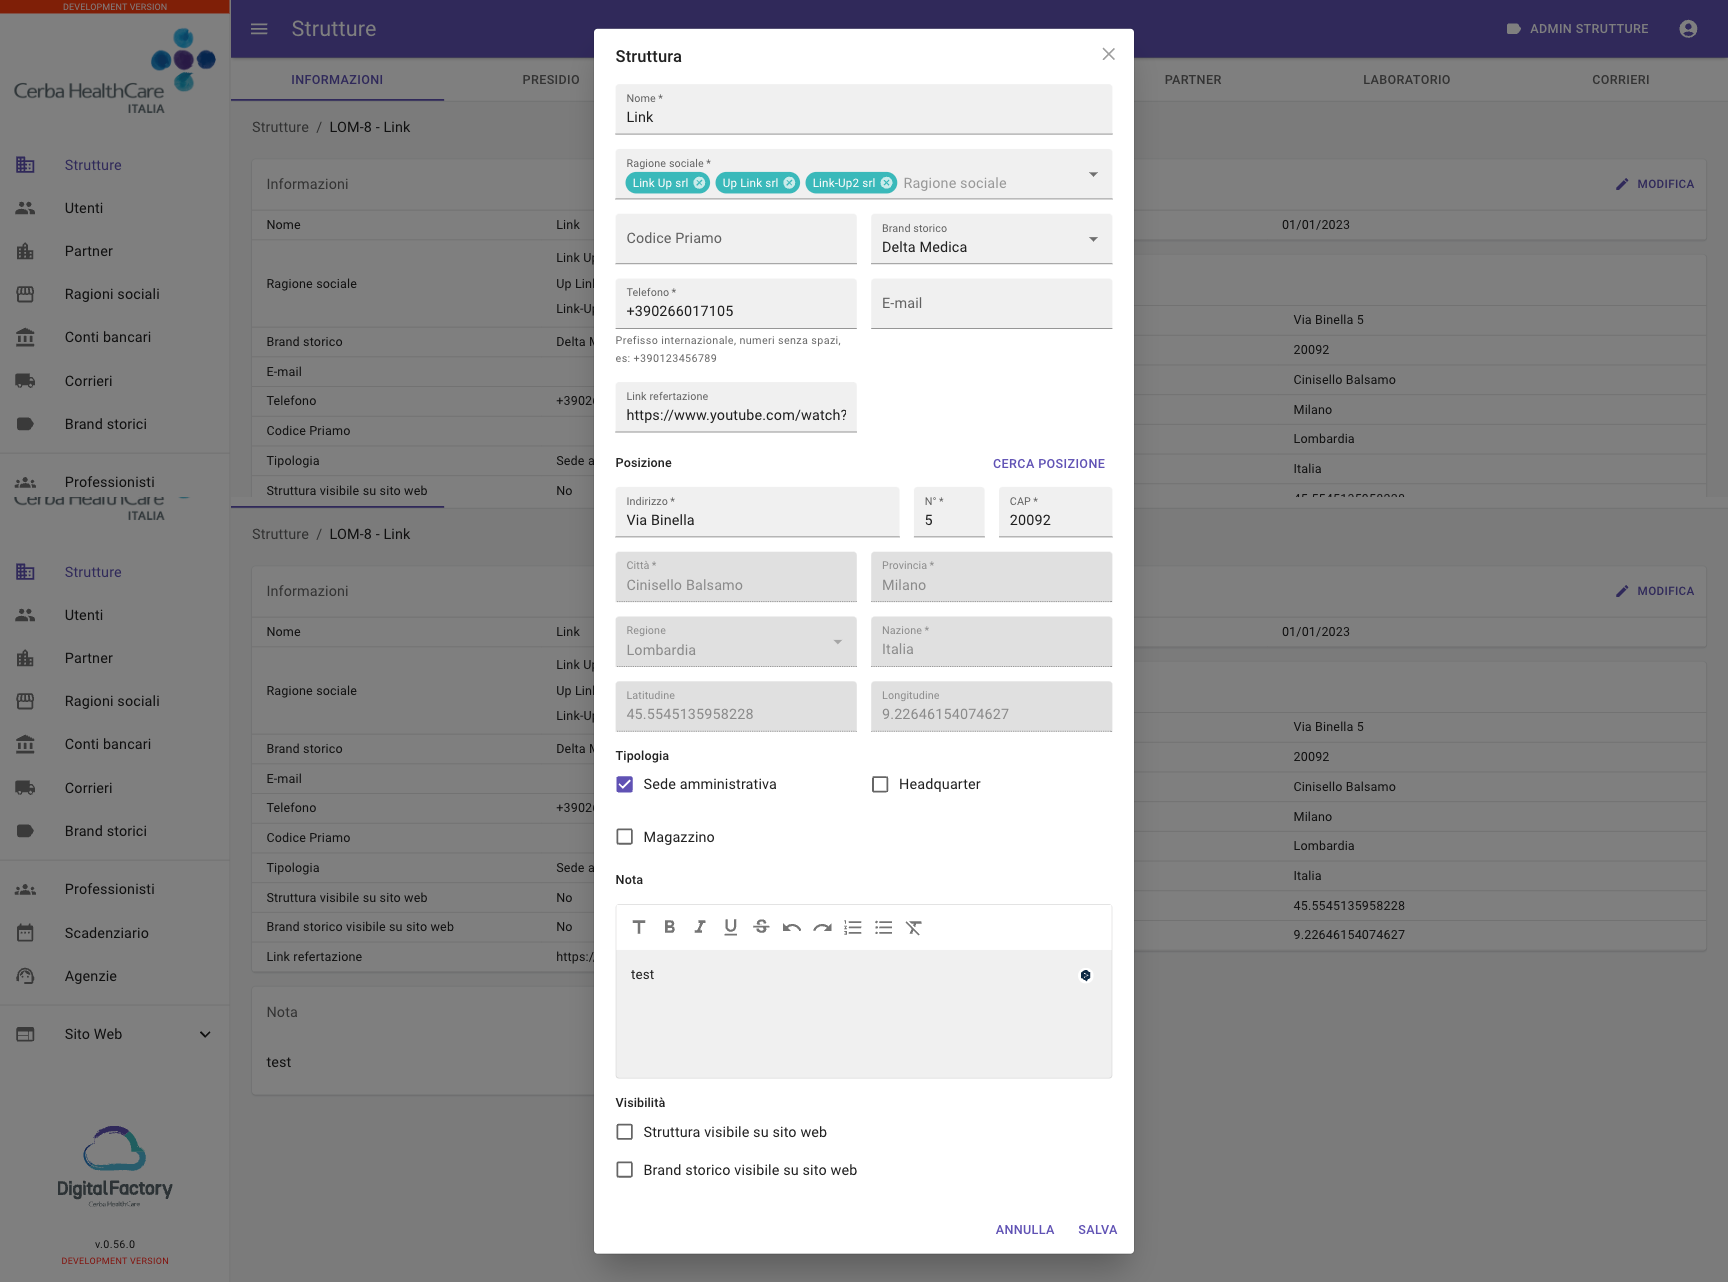
\includegraphics[width= 0.7\textwidth]{images/capitolo5/f1_f2_f3_websiteVisibility_email_links/ModalFacility_edit.png} 
    \caption{Modale modifica struttura esistente} 
    \label{fig:ModalFacility_edit}
\end{figure}

\newpage
\begin{figure}[H]
    \centering
    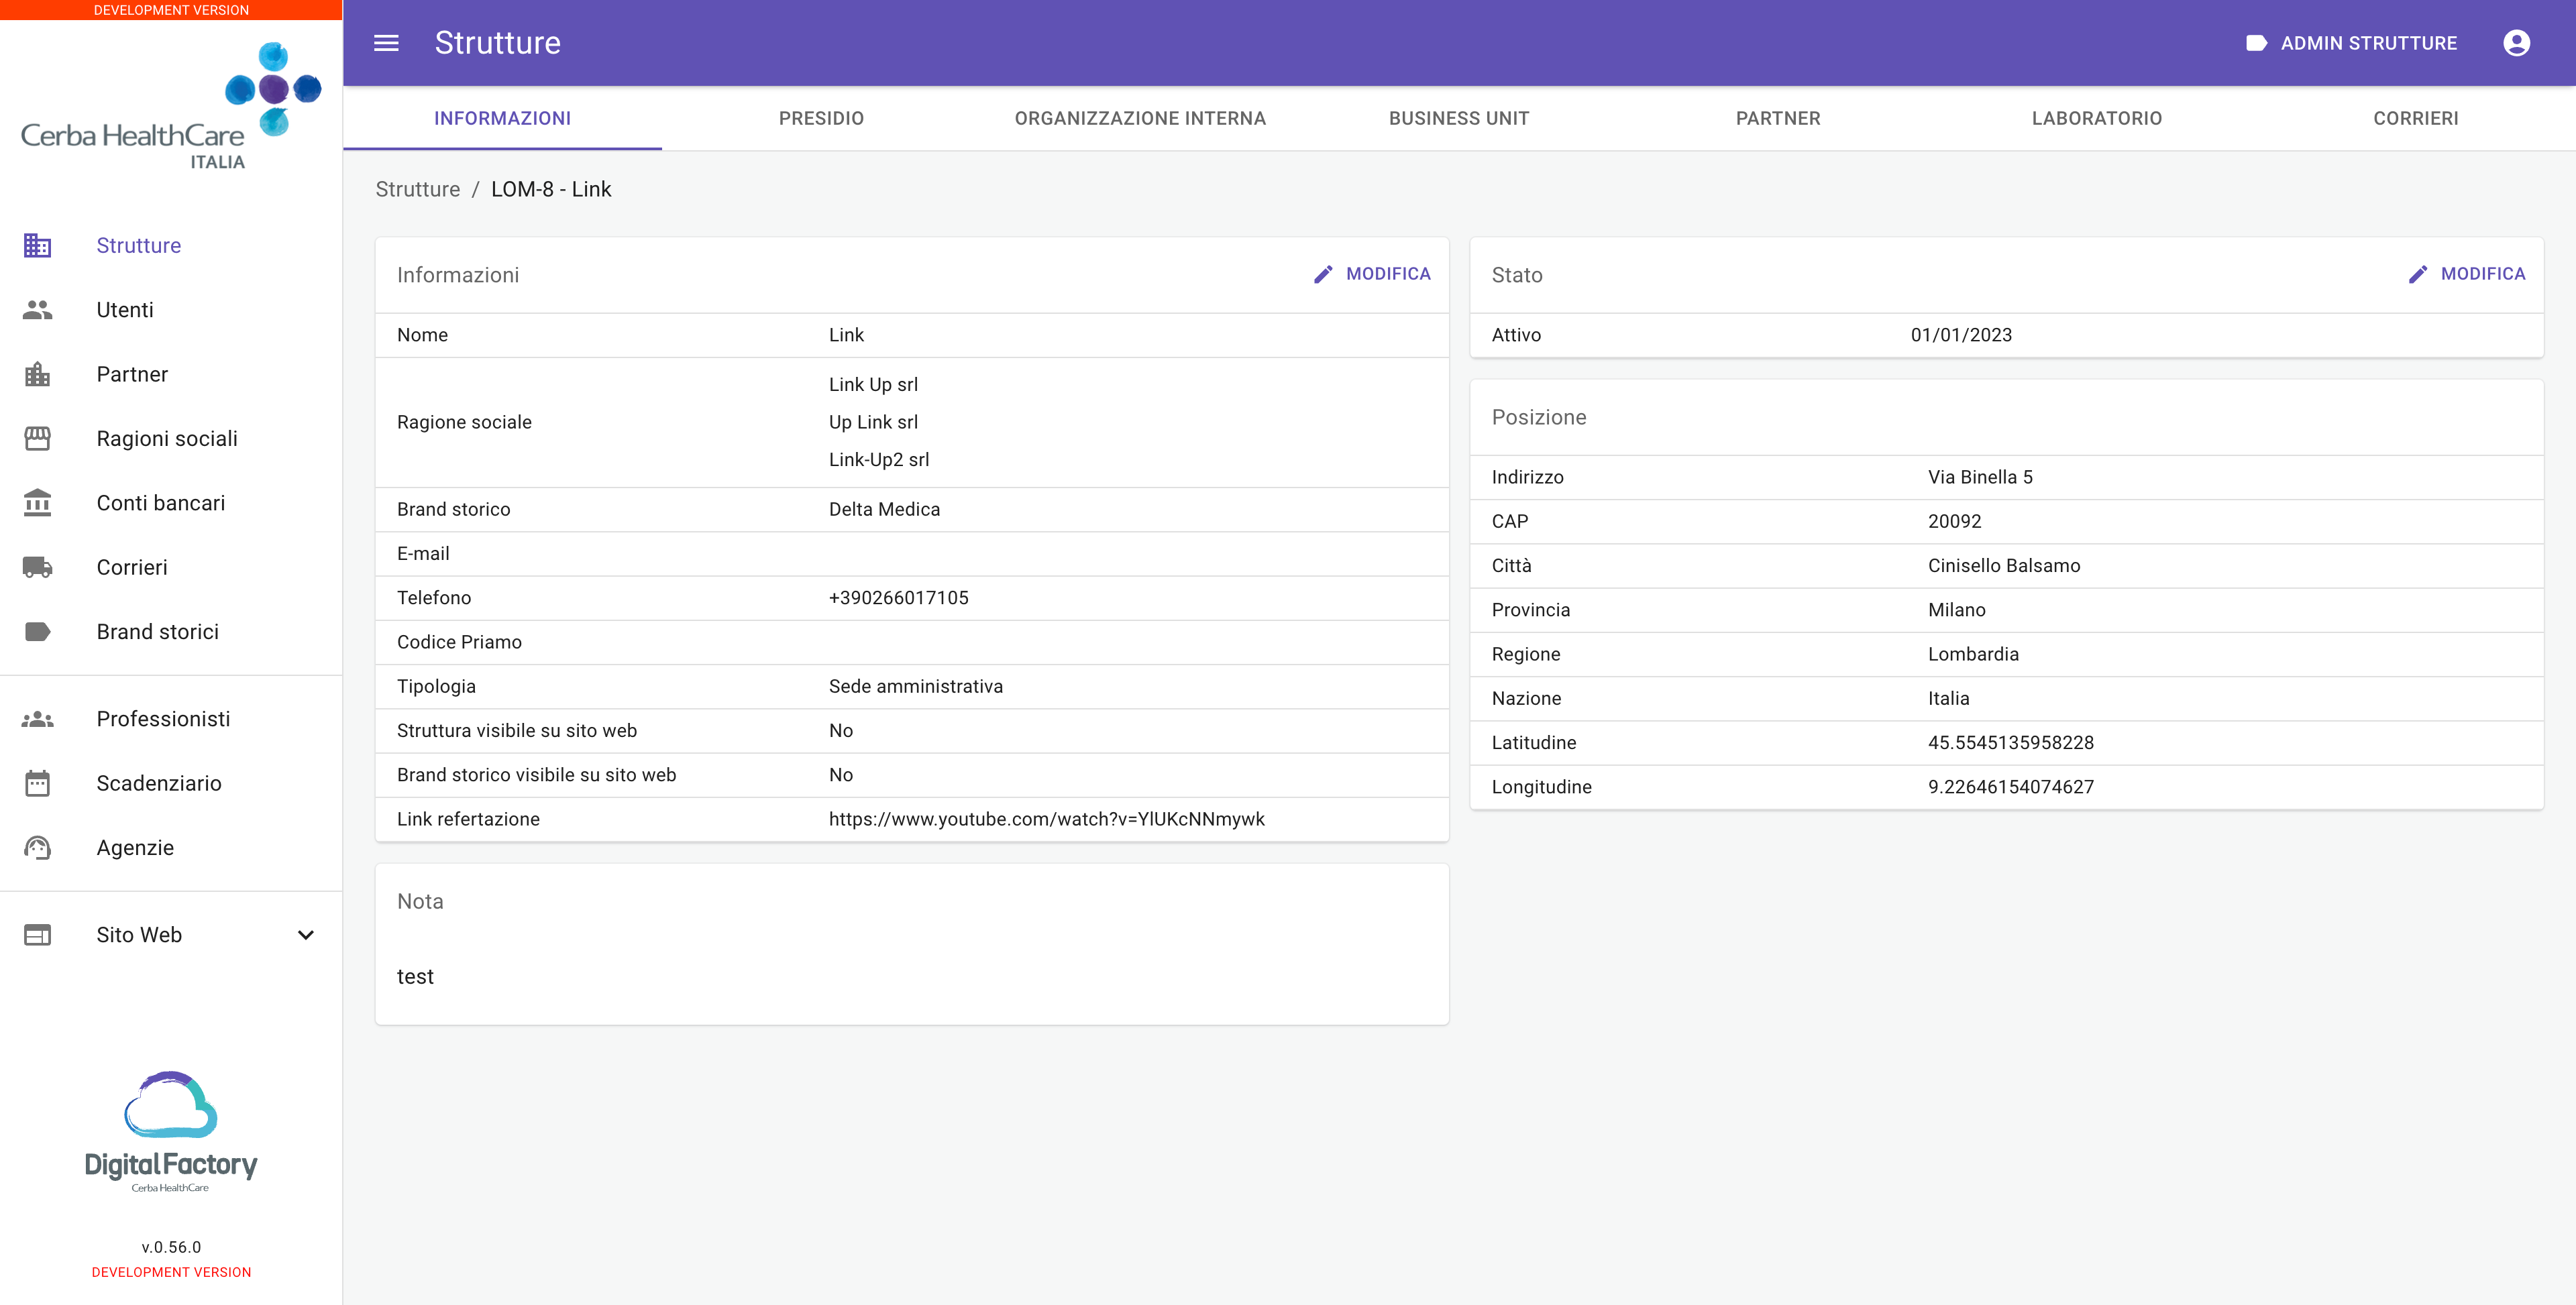
\includegraphics[width= 0.75\textwidth]{images/capitolo5/f1_f2_f3_websiteVisibility_email_links/TabInfo.png} 
    \caption{Tabella informazioni struttura} 
    \label{fig:TabInfo}
\end{figure}

\begin{figure}[H]
    \centering
    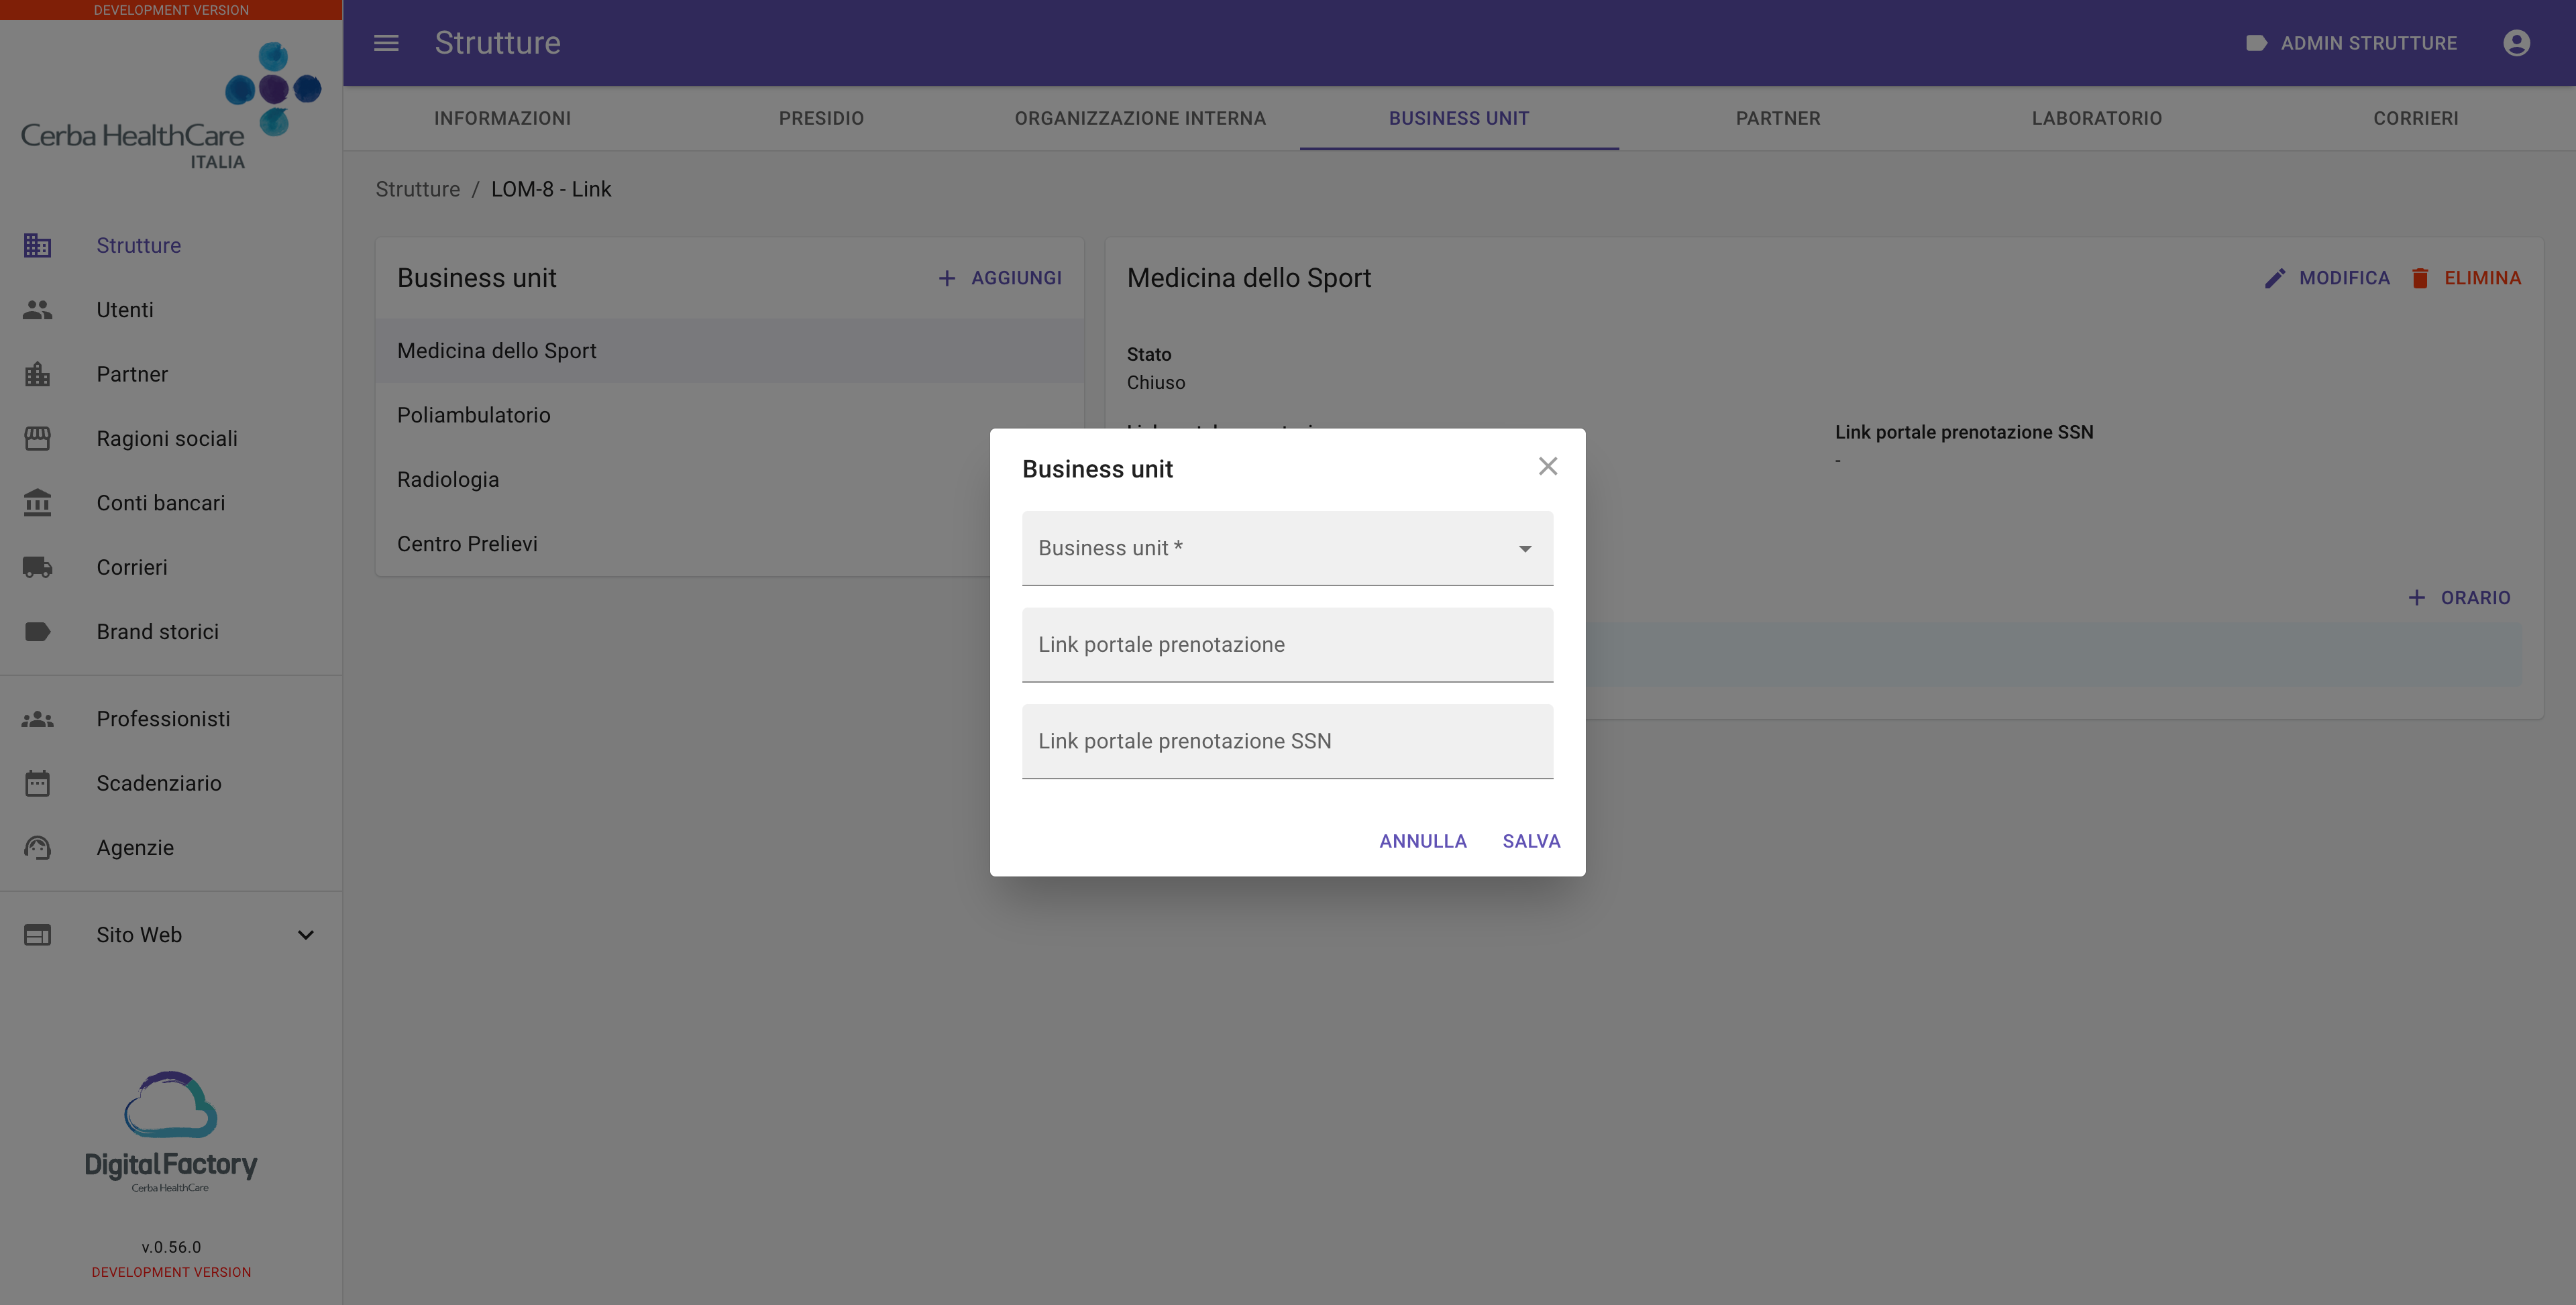
\includegraphics[width= 0.75\textwidth]{images/capitolo5/f1_f2_f3_websiteVisibility_email_links/ModalFacilityBusinessUnit_create.png} 
    \caption{Modale aggiunta nuova BU} 
    \label{fig:ModalFacilityBusinessUnit_create}
\end{figure}

\begin{figure}[H]
    \centering
    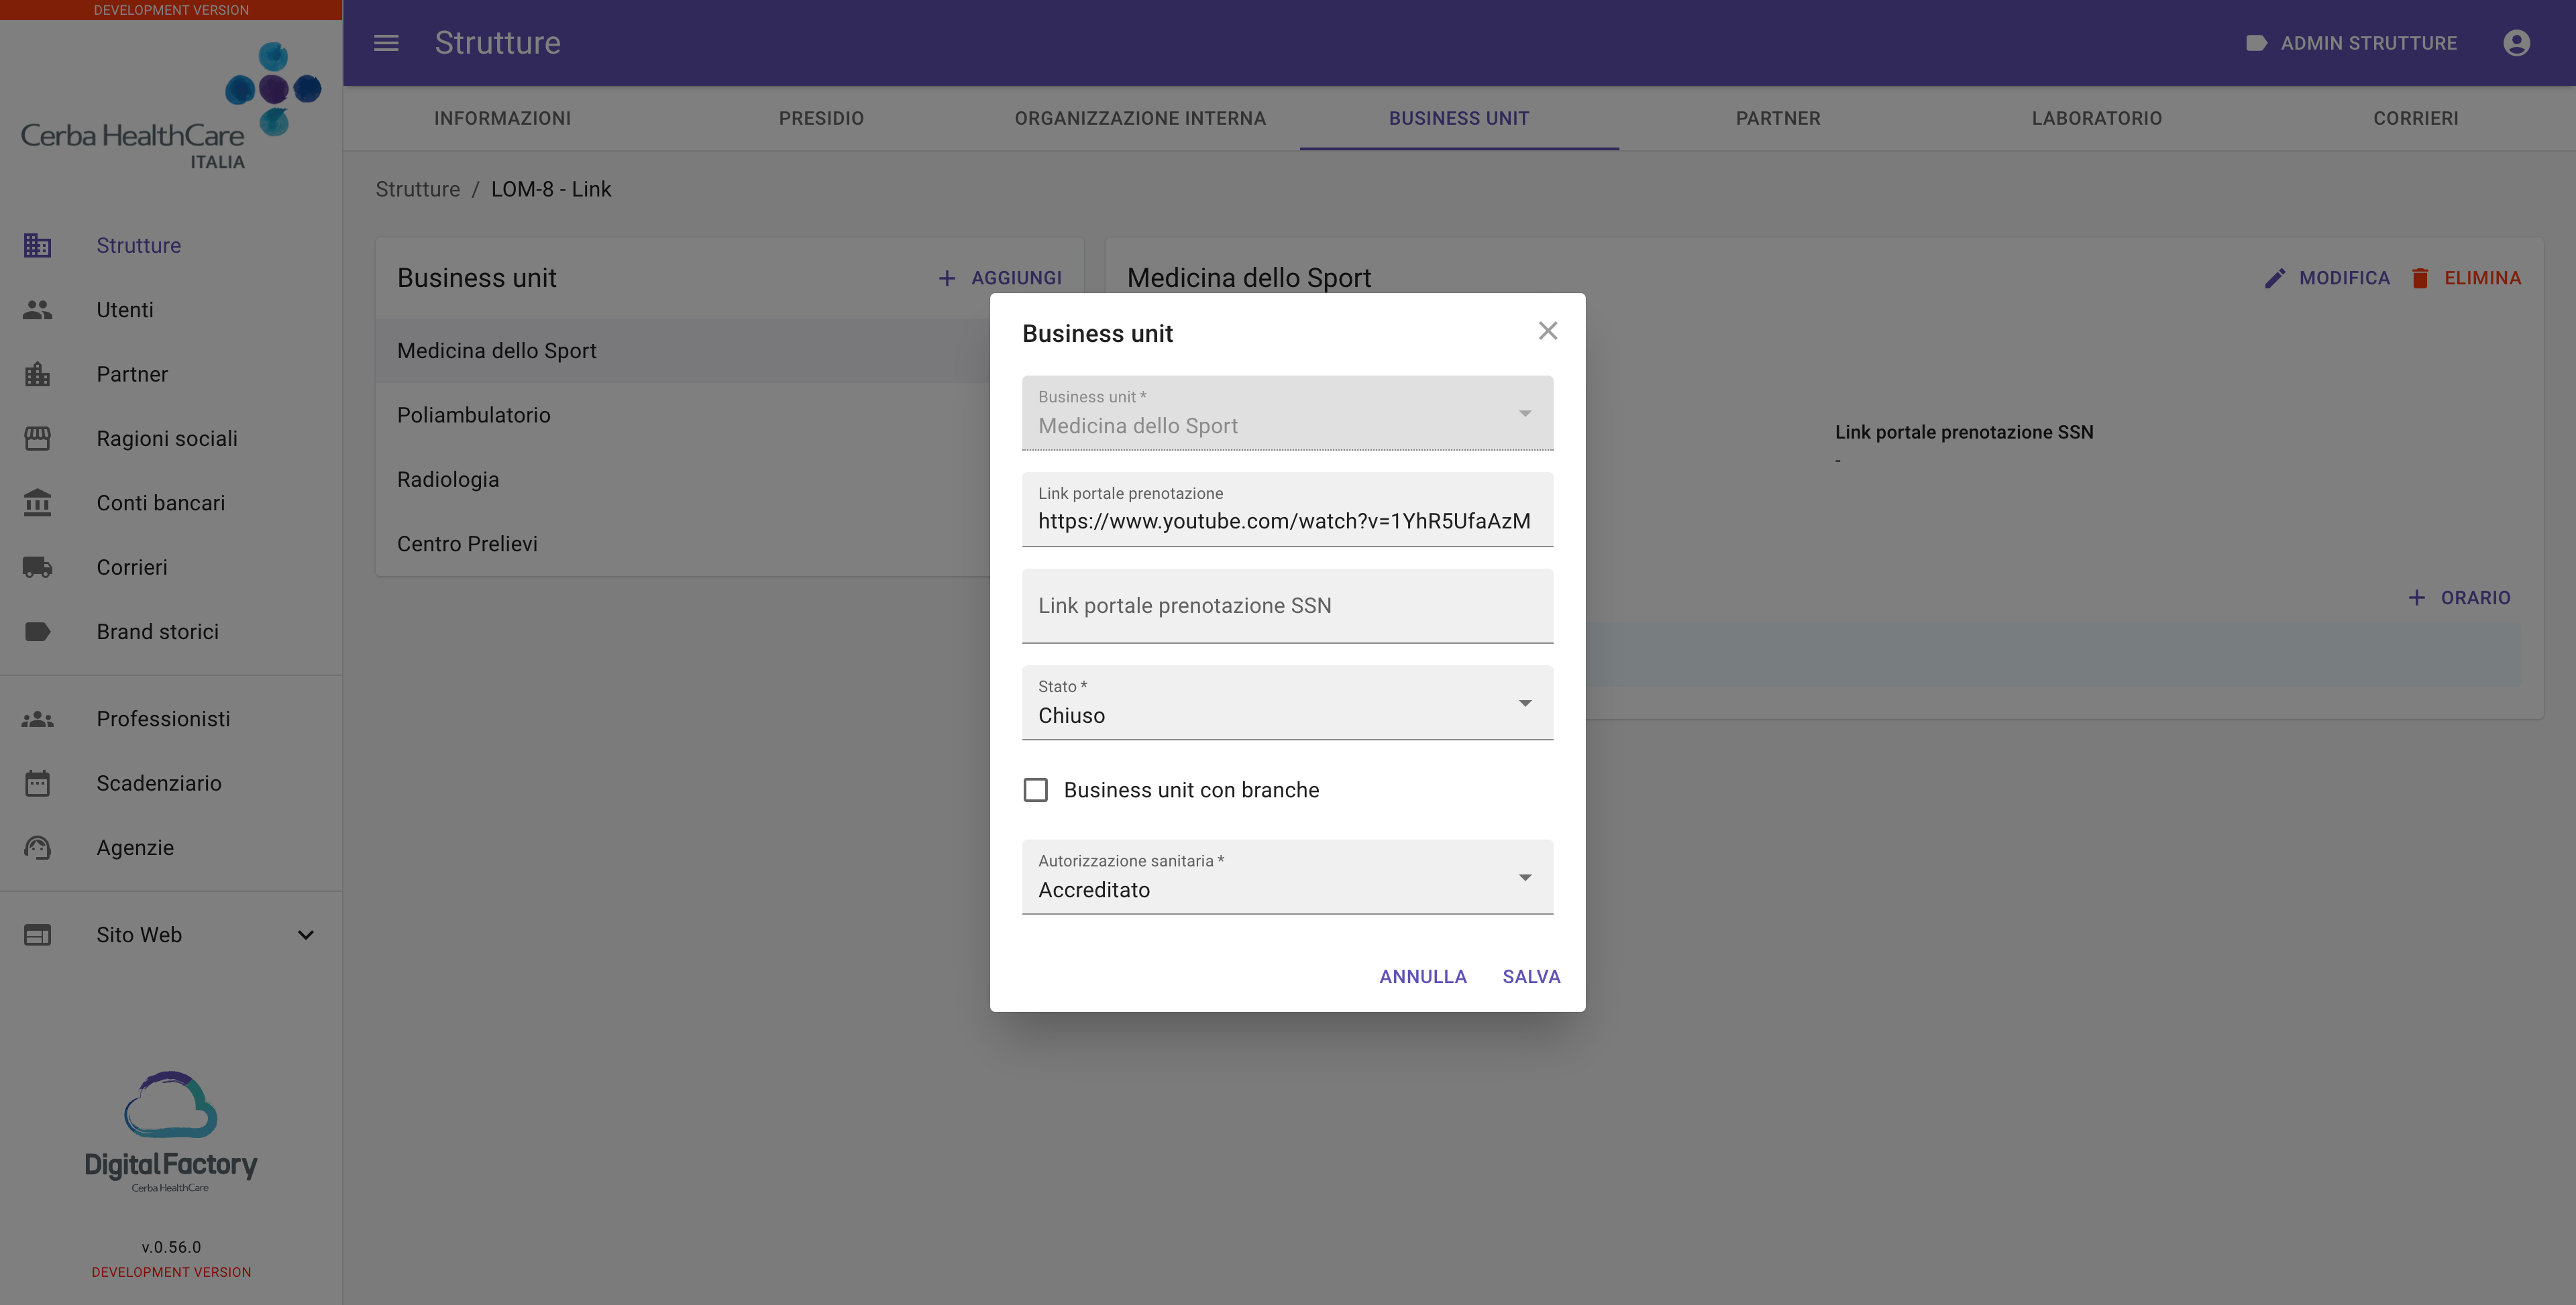
\includegraphics[width= 0.75\textwidth]{images/capitolo5/f1_f2_f3_websiteVisibility_email_links/ModalFacilityBusinessUnit_edit.png} 
    \caption{Modale modifica BU esistente} 
    \label{fig:ModalFacilityBusinessUnit_edit}
\end{figure}

\begin{figure}[H]
    \centering
    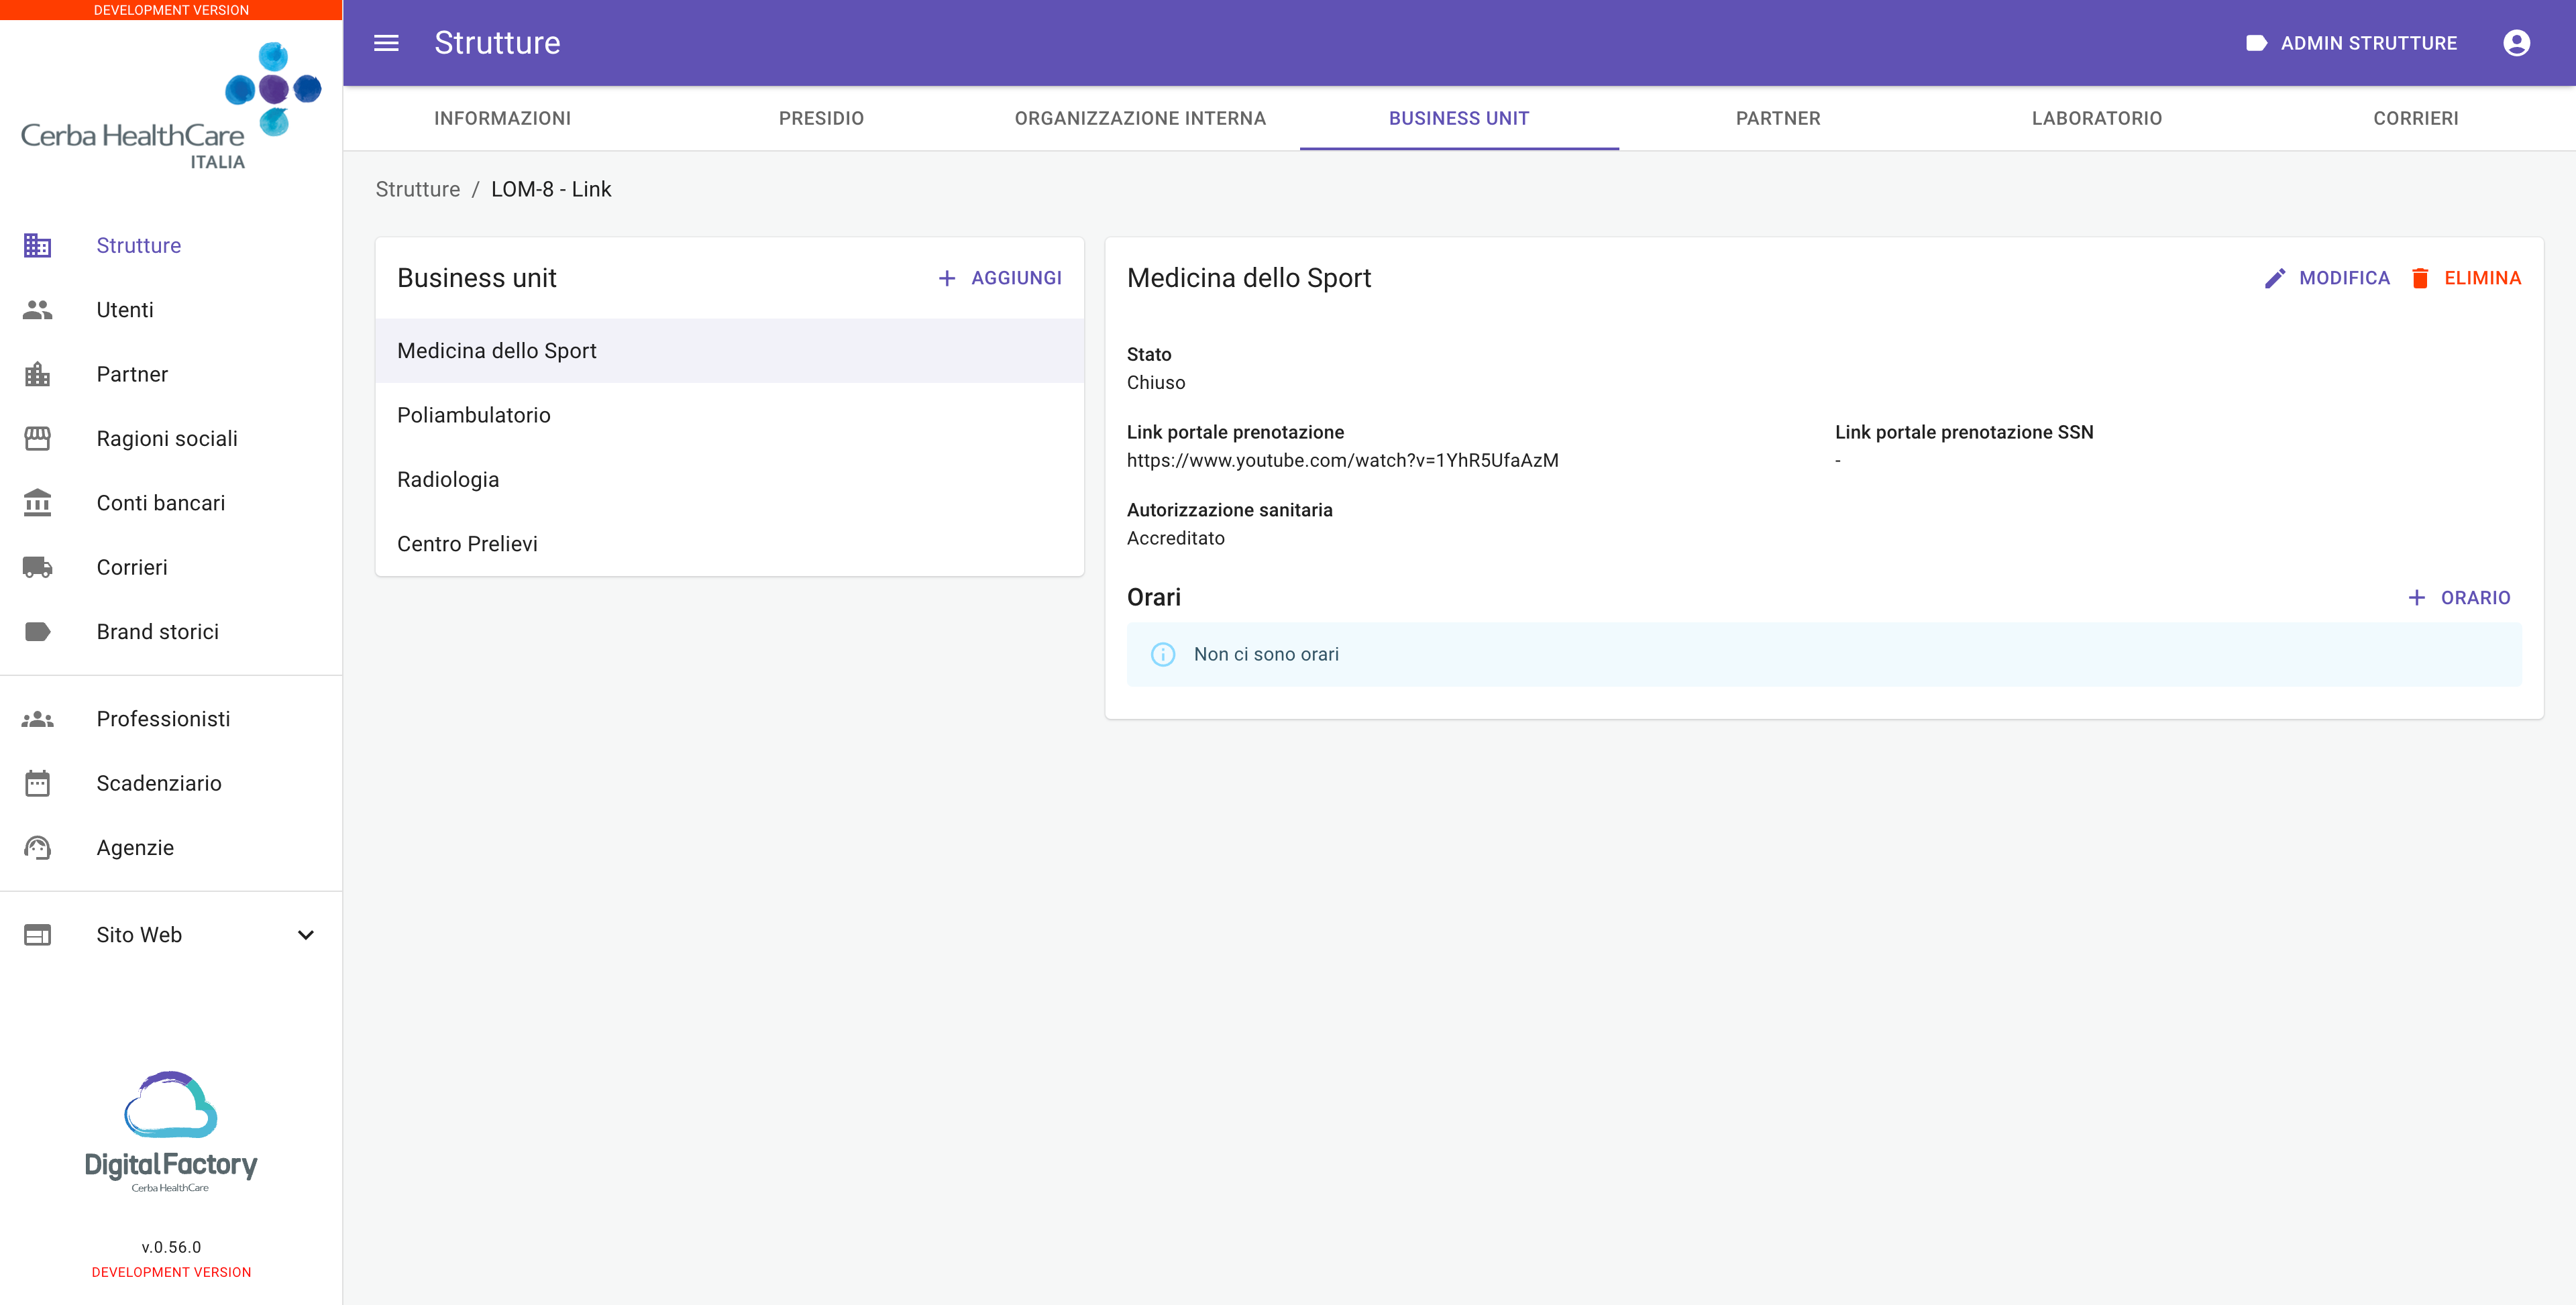
\includegraphics[width= 0.75\textwidth]{images/capitolo5/f1_f2_f3_websiteVisibility_email_links/TabBusinessUnit.png} 
    \caption{Tabella BU esistenti e tabella informazioni BU} 
    \label{fig:TabBusinessUnit}
\end{figure}

% ! PROBLEMA: ordine degli handler, alcuni nelle modali, altri nel componente
\newpage\section{F4: modifica tabella contratti di locazione}
\label{sec:F4: modifica tabella contratti di locazione}
\subparagraph{Requisiti}
La tabella dei contratti di locazione deve essere modificata in modo da poterne visualizzare e gestire di multipli.\\
Deve essere possibile aggiungere e archiviare contratti.\\
La tabella deve mostrare i contratti esistenti in una lista semplice e potersi espandere per mostrare i dettagli di ognuno.

\subparagraph{Procedura}
Il \textbf{primo passo} compiuto è consistito nell'esecuzione delle modifiche riguardanti il funzionamento delle modali. Poiché il codice preesistente permetteva già la modifica dei contratti di locazione esistenti, le introduzioni effettuate hanno riguardato la possibilità di aggiungerne di nuovi e la loro archiviazione.

\textit{In primis}, ciò ha necessitato la creazione delle funzioni \texttt{createRentalAgreement()} e \texttt{deleteRentalAgreement()}, le funzioni che effettuano le chiamate alle \gls{api} visibili nel \autoref{f4_api}. All'interno del loro corpo (alle righe 2 e 5) sono state utilizzate, rispettivamente, le funzioni \texttt{put()} e \texttt{del()}, funzioni che hanno il compito di effettuare richieste avvalendosi dei metodi \texttt{PUT} e \texttt{DELETE}.

\lstinputlisting[caption=Funzioni di chiamata \gls{api} contratti, label=f4_api, language=JSX]{listings/capitolo5/f4_rentalAgreement/api.js}

% ! rivedere
% def handler nel flusso
In secondo luogo, la gestione delle modali ha richiesto, a seconda dei casi, la creazione o l'aggiornamento degli \textit{handler}, le funzioni innescate al click di uno specifico bottone\footnote{Tendenzialmente, nel corpo degli \textit{handler} sono invocate le funzioni che effettuano le chiamate alle \gls{api}.}; questi possono essere divisi in due gruppi a seconda dell'obiettivo che si pongono.\\
Il primo ha come scopo l'apertura della modale ed è formato da \\\texttt{handleCreateRentalAgremment()} e \texttt{handleDeleteRentalAgreement()}, gli \textit{handler} mostrati nel \autoref{f4_RentalAgreement_handlers}, dichiarati all'interno del componente \texttt{RentalAgreement}. Il loro funzionamento è sostanzialmente identico e le operazioni che eseguono sono:
\begin{enumerate}
    \item L'impostazione dei dati della modale, attraverso l'uso del \textit{setter} \texttt{setData()} (alle righe 2 e 9);
    
    \item L'apertura della finestra di dialogo, con l'utilizzo della funzione \texttt{open()} (alle righe 3 e 10).
\end{enumerate}
Le differenze riguardano la modale con cui operano e i dati sui quali essa viene impostata. Infatti, se la funzione \texttt{handleCreateRentalAgreement()} ha a che fare con la finestra di dialogo \texttt{modalRentalAgreement}\footnote{La definizione della variabile della modale \texttt{modalRentalAgreement} non è riportata nel \autoref{f4_RentalAgreement_handlers} perché già parte del codice preesistente.} e ne imposta i dati su un oggetto vuoto, \\\texttt{handleDeleteRentalAgreement()} lavora invece con \texttt{modalConfirmDeleteRentalAgreement} e ne imposta i dati sull'oggetto \texttt{rentalAgreement}\footnote{La funzione \texttt{handleDeleteRentalAgreement()} si aspetta il parametro  \texttt{rentalAgreement} in \textit{input}. Per questo motivo, il valore di \texttt{rentalAgreement} corrisponde all'argomento fornito durante l'invocazione della funzione \texttt{handleDeleteRentalAgreement()}.}.
L'oggetto di quest'ultima finestra di dialogo è stato definito attraverso l'uso dell'\textit{hook} \texttt{useModal()} (a riga 6).

\lstinputlisting[caption=\textit{Handler} apertura modale, label=f4_RentalAgreement_handlers, language=JSX]{listings/capitolo5/f4_rentalAgreement/RentalAgreement_handlers.js}
% spazio
Il secondo gruppo di \textit{handler} ha invece come obiettivo l'effettiva manipolazione dei dati ed è formato da \texttt{handleSaveAgreement()} e \texttt{handleArchiveConfirmRentalAgreement()}.\\
Entrambe le funzioni adempiono al loro compito invocando, all'interno del loro corpo, una delle funzioni di chiamata alle \acrshort{api} definite poco fa.\\
Da un lato, come mostrato nel \autoref{f4_ModalRentalAgreement_handleSaveAgreement}, l'\textit{handler} \texttt{handleSaveAgreement()} (già esistente all'interno del componente \texttt{ModalRentalAgreement} in passato) è stato aggiornato con l'introduzione della possibilità di aggiungere un nuovo contratto di locazione. La già esistente riga di codice atta alla gestione della modifica dei contratti, infatti, è stata resa parte di una condizione che si avvale della sintassi \texttt{if...else} (da riga 3 a 7) per esprimere il seguente concetto: se è presente la proprietà \texttt{uuid} dell'oggetto \texttt{rentalAgreement} esegui la funzione \texttt{editRentalAgreement()} passandole come parametri la proprietà \texttt{uuid} stessa e la variabile \texttt{body}; in caso contrario esegui la funzione \texttt{createRentalAgreement()} passandole come parametri le variabili \texttt{uuidFacility} e \texttt{body}.\\
In altre parole, se esiste un contratto di locazione eseguine la modifica, altrimenti creane uno nuovo.

\lstinputlisting[caption=\textit{Handler} aggiunta nuovo contratto, label=f4_ModalRentalAgreement_handleSaveAgreement, language=JSX]{listings/capitolo5/f4_rentalAgreement/ModalRentalAgreement_handleSaveAgreement.js}
% spazio
Dall'altro lato, come illustrato nel \autoref{f4_RentalAgreement_handleArchiveConfirmRentalAgreement}, è stato creato, di nuovo all'interno del componente \texttt{RentalAgreement}, l'\textit{handler} \texttt{handleArchiveConfirmRentalAgreement()} per l'archiviazione dei contratti di locazione. Questo esegue l'archiviazione del contratto, grazie alla funzione \texttt{deleteRentalAgreement()}, e l'aggiornamento della lista dei contratti di locazione, tramite \texttt{fetchRentalAgreements()}.

\lstinputlisting[caption=\textit{Handler} archiviazione contratto, label=f4_RentalAgreement_handleArchiveConfirmRentalAgreement, language=JSX]{listings/capitolo5/f4_rentalAgreement/RentalAgreement_handleArchiveConfirmRentalAgreement.js}

Il \textbf{secondo passo} compiuto, invece, è consistito nell'aggiornamento della \acrshort{ui} del componente \texttt{RentalAgreement}, elemento responsabile dell'intera tabella dei contratti di locazione.

Come possibile vedere nel \autoref{f4_RentalAgreement_UI}, un componente \texttt{Card} (da riga 2 a 28) è stato utilizzato per racchiudere tutti i componenti figli che formano la struttura della tabella.\\
\texttt{CardHeader}, il primo di essi, ha come compito il \textit{rendering} dell'\textit{header} e le sue \textit{props} sono: 
\begin{itemize}
    \item \texttt{subheader} (a riga 4): il suo valore è la stringa \texttt{"Contratti locazione"};
    \item \texttt{action} (da riga 5 a 12): il suo valore è il componente \texttt{Button}, il quale racchiude il testo “Aggiungi” ed è dotato, a sua volta, delle \textit{props}:
        \begin{itemize}
            \item \texttt{onClick}: il suo valore è l'\textit{handler} \texttt{handleCreateRentalAgreement};
            \item \texttt{startIcon}: il suo valore è il componente \texttt{AddIcon}.
        \end{itemize}
\end{itemize}
Il secondo componente figlio di \texttt{Card} è \texttt{Divider} (a riga 15), elemento che stabilisce un confine fra l'\textit{header} e tutto ciò che sta al di sotto di lui.\\
La struttura di \texttt{Card} termina con il componente \texttt{Table}, terzo ed ultimo elemento che si occupa del \textit{rendering} del corpo della tabella (da riga 18 a 29). Questo racchiude un componente \texttt{TableBody} all'interno del quale viene effettuato un \textit{mapping}: l'iteratore \texttt{map()} è utilizzato sull'\textit{array} \texttt{rentalAgreements} affinché tutti gli oggetti che lo compongono vengano visualizzati grazie all'istanza del componente \texttt{TabBuildingRentalAgreementTable}. Le \textit{props} passate a quest'ultima sono: 
\begin{itemize}
    \item \texttt{key}: il suo valore è la proprietà \texttt{uuid} dell'oggetto \texttt{el};
    
    \item \texttt{el}: il singolo contratto che, di volta in volta, viene mappato sul componente. Il suo valore è l'oggetto \texttt{el};
    
    \item \texttt{handleEditRentalAgreement}: il suo valore è l'\textit{handler} \texttt{handleEditRentalAgreement()};
    
    \item \texttt{handleDeleteRentalAgreement}: il suo valore è l'\textit{handler} \texttt{handleDeleteRentalAgreement()}.
\end{itemize}
Le ultime due \textit{props} forniscono le funzioni invocate dai bottoni contenuti nel componente.

Inoltre, è stato necessario introdurre il componente \texttt{ModalConfirm}, elemento responsabile della restituzione dell'ulteriore finestra di dialogo che compare per chiedere all'utente la conferma prima di eseguire l'archiviazione di un contratto.\\
Tramite una condizione che si avvale dell'operatore logico AND (da riga 32 a 39) viene stabilito che, se il valore della proprietà \texttt{isOpen} dell'oggetto \\\texttt{modalConfirmDeleteRentalAgreement} è vero, allora viene eseguito il \textit{rendering} del componente. In tal caso, le \textit{props} fornite a \texttt{ModalConfirm} sono: 
\begin{itemize}
    \item \texttt{modal}: il suo valore è l'oggetto \texttt{modalConfirmDeleteRentalAgreement};
    \item \texttt{title}: il suo valore è la stringa \texttt{'Archivia contratto locazione'};
    \item \texttt{text}: il suo valore è un'espressione che stabilisce la composizione di una stringa; 
    \item \texttt{handleConfirm}: il suo valore è l'\textit{handler} \texttt{handleArchiveConfirmRentalAgreement()}.
\end{itemize}
La funzione passata alla \textit{prop} \texttt{handleConfirm} è quella che viene invocata dal bottone del componente.

\lstinputlisting[caption=Tabella contratti esistenti, label=f4_RentalAgreement_UI, language=JSX]{listings/capitolo5/f4_rentalAgreement/RentalAgreement_UI.js}

Il \textbf{terzo passo} è consistito nella gestione del corpo della tabella per la visualizzazione delle informazioni dei contratti di locazione. 
Ciò è stato fatto attraverso l'implementazione di un nuovo componente creato \textit{ad hoc}, \texttt{TabBuildingRentalAgreementTable}, del quale era stata utilizzata precedentemente l'istanza all'interno del \textit{mapping}.\\
Come prassi vuole, la definizione di tale elemento ha previsto l'importazione delle \textit{props} passate alla sua istanza; il \autoref{f4_TabBuildingRentalAgreementTable_component} mostra che ciò è stato fatto, attraverso la tecnica della destrutturazione, per \texttt{el}, \texttt{handleEditRentalAgreement()} e \texttt{handleDeleteRentalAgreement()} (a riga 2).

\lstinputlisting[caption=Componente \texttt{TabBuildingRentalAgreementTable}, label=f4_TabBuildingRentalAgreementTable_component, language=JSX]{listings/capitolo5/f4_rentalAgreement/TabBuildingRentalAgreementTable_component.js}

Anche in questo caso, delle modifiche a livello di logica hanno costituito lo \textit{step} iniziale. Poiché fra i requisiti era presente l'espandibilità di ogni riga della tabella, la definizione del componente è stata seguita dalla gestione di questa dinamica\footnote{La gestione della dinamica di espansione è stata effettuata all'interno del corpo del componente \texttt{TabBuildingRentalAgreementTable}.}, che viene illustrara nel \autoref{f4_TabBuildingRentalAgreementTable_dynamic}.\\
Il concetto di espansione è stato implementato grazie alla variabile di stato \texttt{toggleOpen} e al relativo \textit{setter} \texttt{setToggleOpen()}, dichiarati attraverso l'\textit{hook} \texttt{useState()} (a riga 1). Poiché, salvo click da parte dell'utente, le righe della tabella appaiono nella pagina come non espanse, \texttt{toggleOpen} è stata inizializzata con il valore booleano \texttt{false}.\\
Inoltre, è possibile vedere l'\textit{handler} \texttt{handleOpenRentalAgreement}, la funzione responsabile del funzionamento del meccanismo di espansione. Questa sfrutta il \textit{setter} \texttt{setToggleOpen()} per sostituire il precedente valore della variabile di stato \texttt{toggleOpen} con il suo opposto ogni volta che viene invocata.

\lstinputlisting[caption=Dinamica apertura riga tabella contratti, label=f4_TabBuildingRentalAgreementTable_dynamic, language=JSX]{listings/capitolo5/f4_rentalAgreement/TabBuildingRentalAgreementTable_dynamic.js}

Il \textbf{quarto} e \textbf{ultimo} passo è consistito nella creazione della \acrshort{ui} del neonato componente \texttt{TabBuildingRentalAgreementTable}.

Il \autoref{f4_TabBuildingRentalAgreementTable_UI} mostra come il tag padre \texttt{<>} sia stato utilizzato come contenitore per due grandi componenti figli \texttt{TableRow}. Questi costituiscono le due righe che, di volta in volta, racchiudono le informazioni dei contratti di locazione esistenti. Se la prima deve permettere all'utente di visualizzare, anche senza l'espansione della riga, solo alcuni dati del contratto e i bottoni per la sua gestione, la seconda deve invece mostrare, una volta espansa la riga, tutte le informazioni del contratto nel dettaglio.\\
Entrambi i componenti \texttt{TableRow} contengono, a loro volta, molti elementi figli; all'interno del primo (da riga 2 a 41) sono presenti quattro componenti \texttt{TableCell}:
\begin{itemize}
    \item \texttt{TableCell} (da riga 3 a 7): contiene il componente \texttt{Typography} che effettua il \textit{rendering} di un sottotitolo. Il sottotitolo ritornato è quello risultante dalla condizione che si avvale dell'operatore ternario (a riga 5); questa esprime il seguente concetto: se la proprietà \texttt{label} dell'oggetto \texttt{type} (contenuto dall'oggetto \texttt{el}) è vera, allora restituisci tale proprietà, altrimenti una stringa dal valore \texttt{'-'};
    
    \item \texttt{TableCell} (a riga 9): contiene una condizione che si avvale dell'operatore logico AND per esprimere il seguente concetto: solo se la proprietà \texttt{archived} dell'oggetto \texttt{el} è vera, restituisci la stringa \texttt{'(archiviato)'};
    
    \item \texttt{TableCell} (da riga 11 a 25): contiene il componente \texttt{Button}, il bottone necessario all'espansione della riga. Le su \textit{props} più importanti sono:
    \begin{itemize}
        \item \texttt{onClick} (a riga 14): il suo valore è \texttt{handleOpenRentalAgreement()};
        
        \item \texttt{startIcon} (a riga 15): il suo valore è una condizione che si avvale dell'operatore ternario per esprimere il seguente concetto: se la variabile di stato \texttt{toggleOpen} ha come valore il \texttt{true}, restituisci il componente \texttt{KeyBoardArrowUpIcon}, altrimenti \texttt{KeyBoardArrowDownIcon}. In altre parole, se la riga è espansa restituisci una freccia che punta verso l'alto, altrimenti, una freccia che punta verso il basso.\\
        All'interno del componente viene effettuato il \textit{rendering} del testo “Mostra”;
    \end{itemize}

    \item \texttt{TableCell} (da riga 27 a 40): contiene due componenti \texttt{IconButton}, ovvero i bottoni atti alla manipolazione dei contratti di locazione. Entrambi sono dotati della \textit{prop} \texttt{onClick}, il cui valore è però diverso a seconda della casistica: quello del bottone che si occupa della modifica è l'\textit{handler} \texttt{handleEditRentalAgreement()}, mentre quello del bottone atto all'archiviazione è \texttt{handleDeleteRentalAgreement()}. A entrambe le funzioni viene passato come argomento l'oggetto \texttt{el}, il contratto che di volta in volta sarà modificato o archiviato.\\
    Inoltre, il bottone per la modifica contiene il componente \texttt{EditIcon}, mentre quello per l'archiviazione \texttt{DeleteIcon}.
\end{itemize}
% spazio
All'interno del secondo componente \texttt{TableRow} (da riga 43 a 60) è invece presente un solo \texttt{TableCell} che contiene a sua volta il componente \texttt{Collapse} (da riga 45 a 58), elemento il cui compito è l'effettiva gestione della dinamica di apertura e chiusura della riga della tabella; ciò avviene grazie alla \textit{prop} \texttt{in}, il cui valore è la variabile di stato \texttt{toggleOpen}.

Le informazioni dettagliate di ogni contratto di locazione vengono mostrate attraverso un'ulteriore tabella, visibile solamente a riga espansa, contenuta dal componente \texttt{TableBody}\footnote{La struttura della tabella, incomincia in realtà con il componente \texttt{TableContainer} (da riga 46 a 57).}. Questo è composto da tanti componenti \texttt{TableRow} quante sono le proprietà dell'oggetto \texttt{el}, ovvero, quante sono le informazioni del contratto che si desidera vengano mostrate all'interno della tabella. Ogni riga è formata a sua volta da due componenti \texttt{TableCell}, una cella per la visualizzazione del tipo di informazione riportata, e una per il dato associato al tipo di informazione. 

\lstinputlisting[caption=Riga tabella contratti, label=f4_TabBuildingRentalAgreementTable_UI, language=JSX]{listings/capitolo5/f4_rentalAgreement/TabBuildingRentalAgreementTable_UI.js}

\paragraph{\textit{Output} grafico}
\begin{figure}[H]
    \centering
    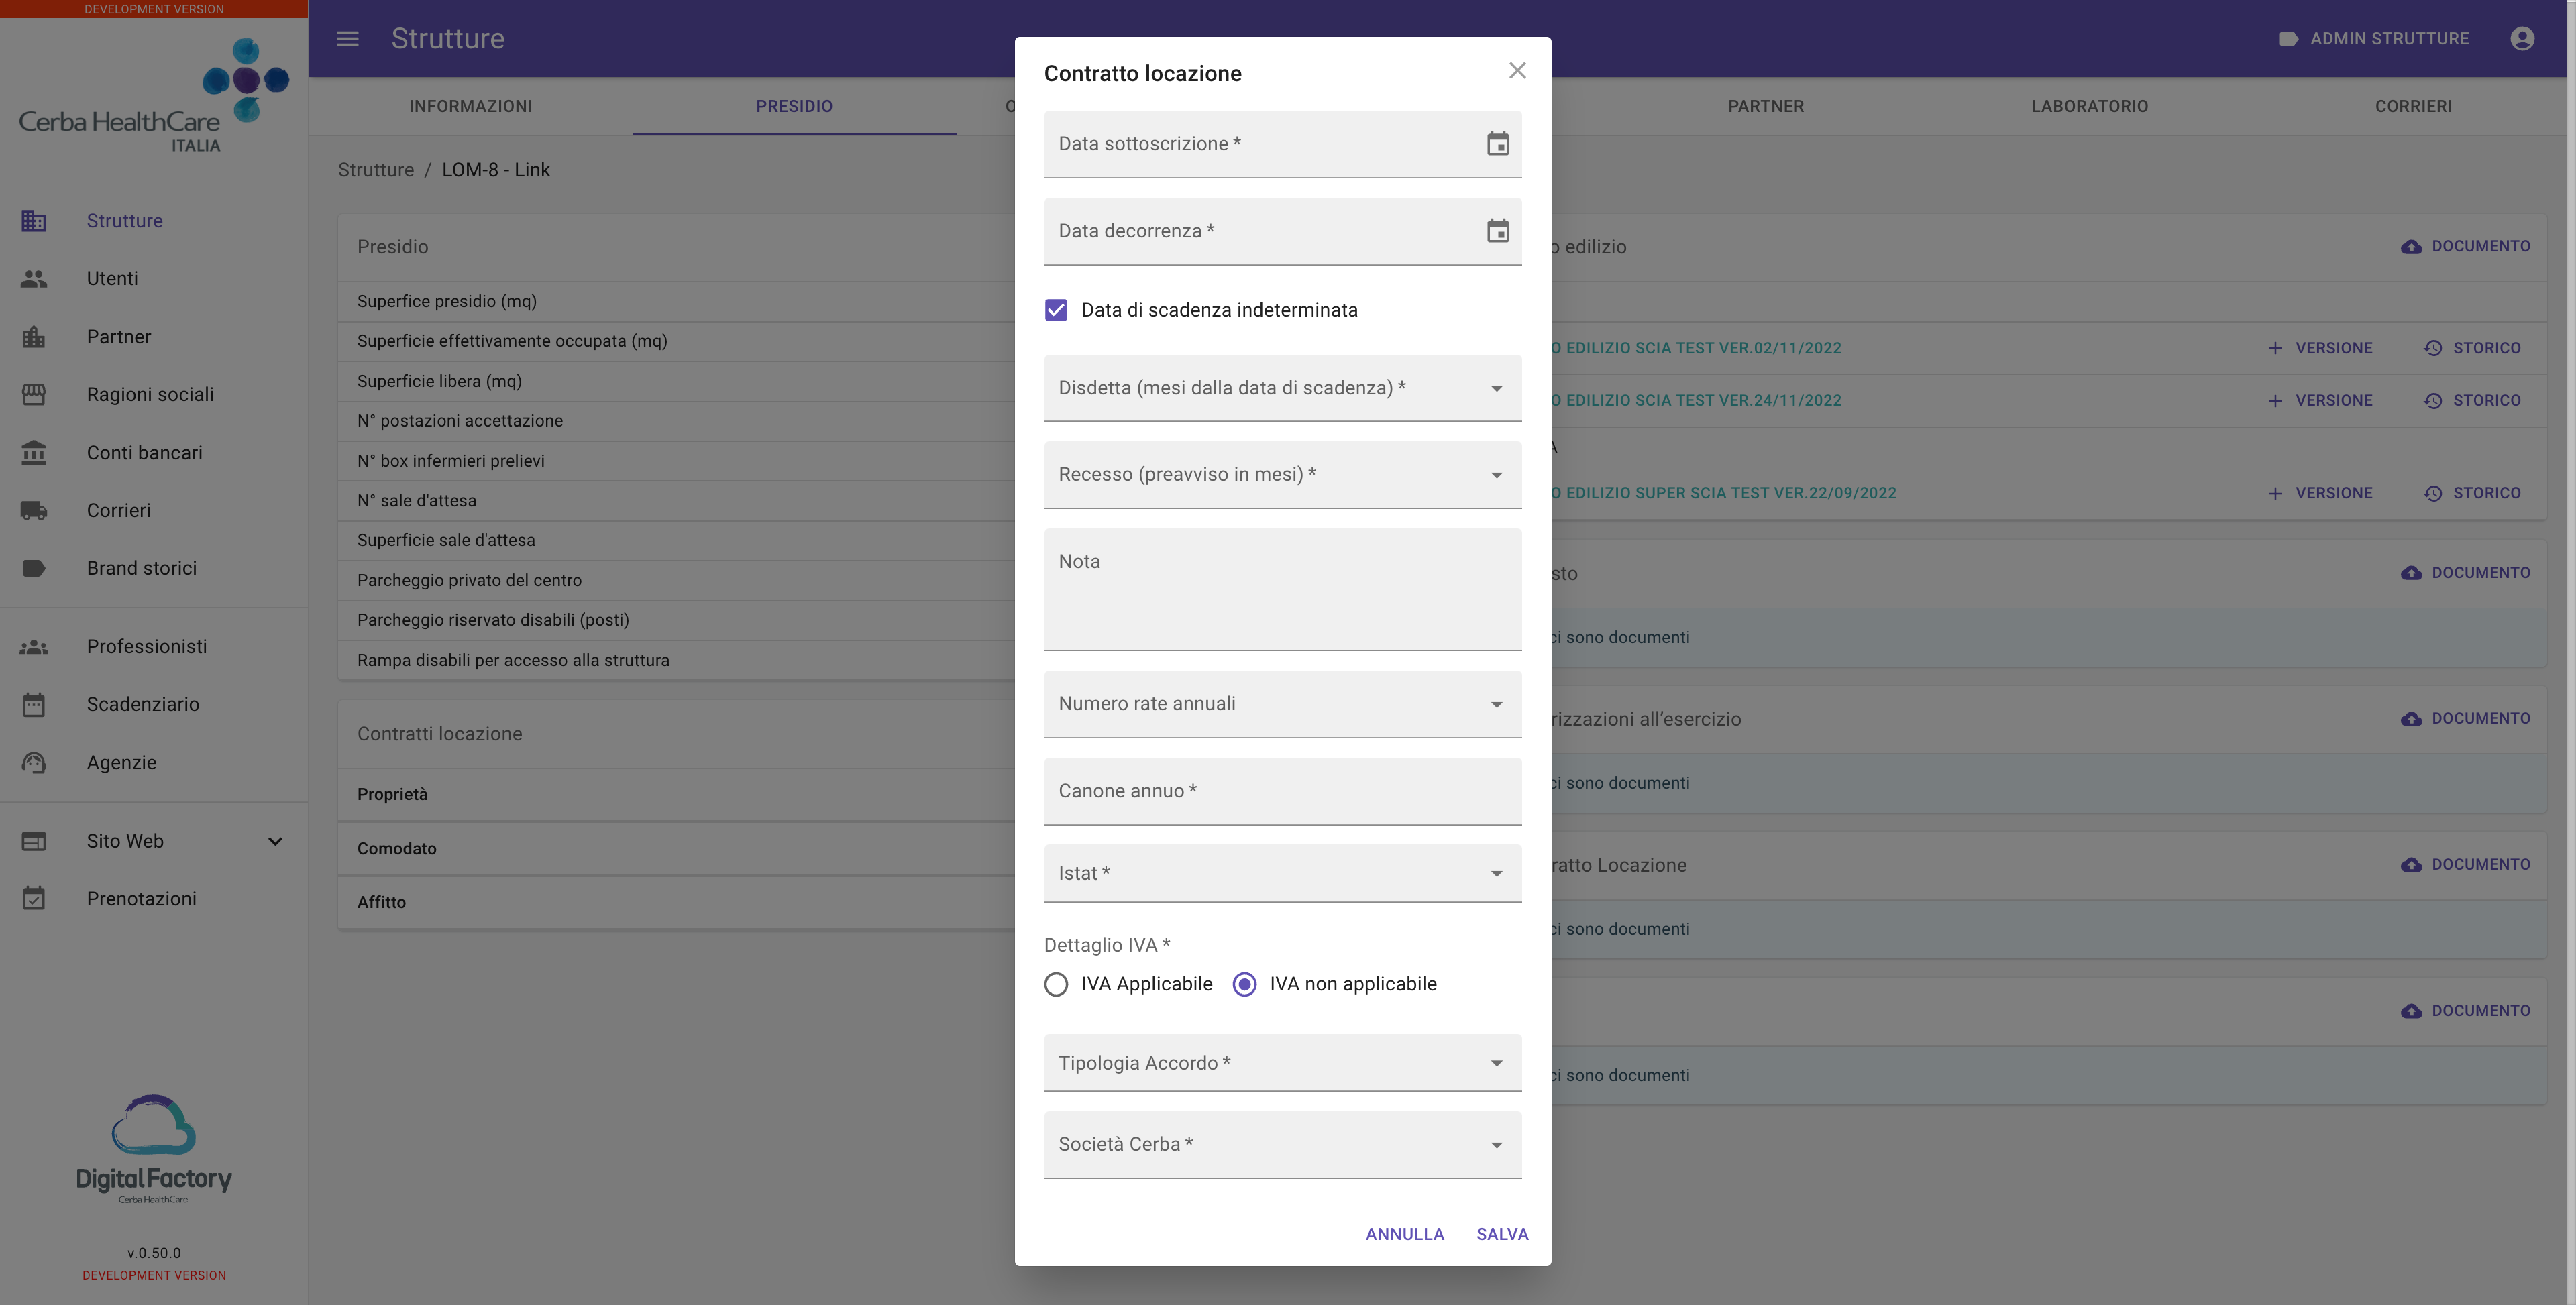
\includegraphics[width=0.75\textwidth]{images/capitolo5/f4_rentalAgreement/RentalAgreement_create.png} 
    \caption{Modale aggiunta nuovo contratto} 
    \label{fig:RentalAgreement_create}
\end{figure}

\begin{figure}[H]
    \centering
    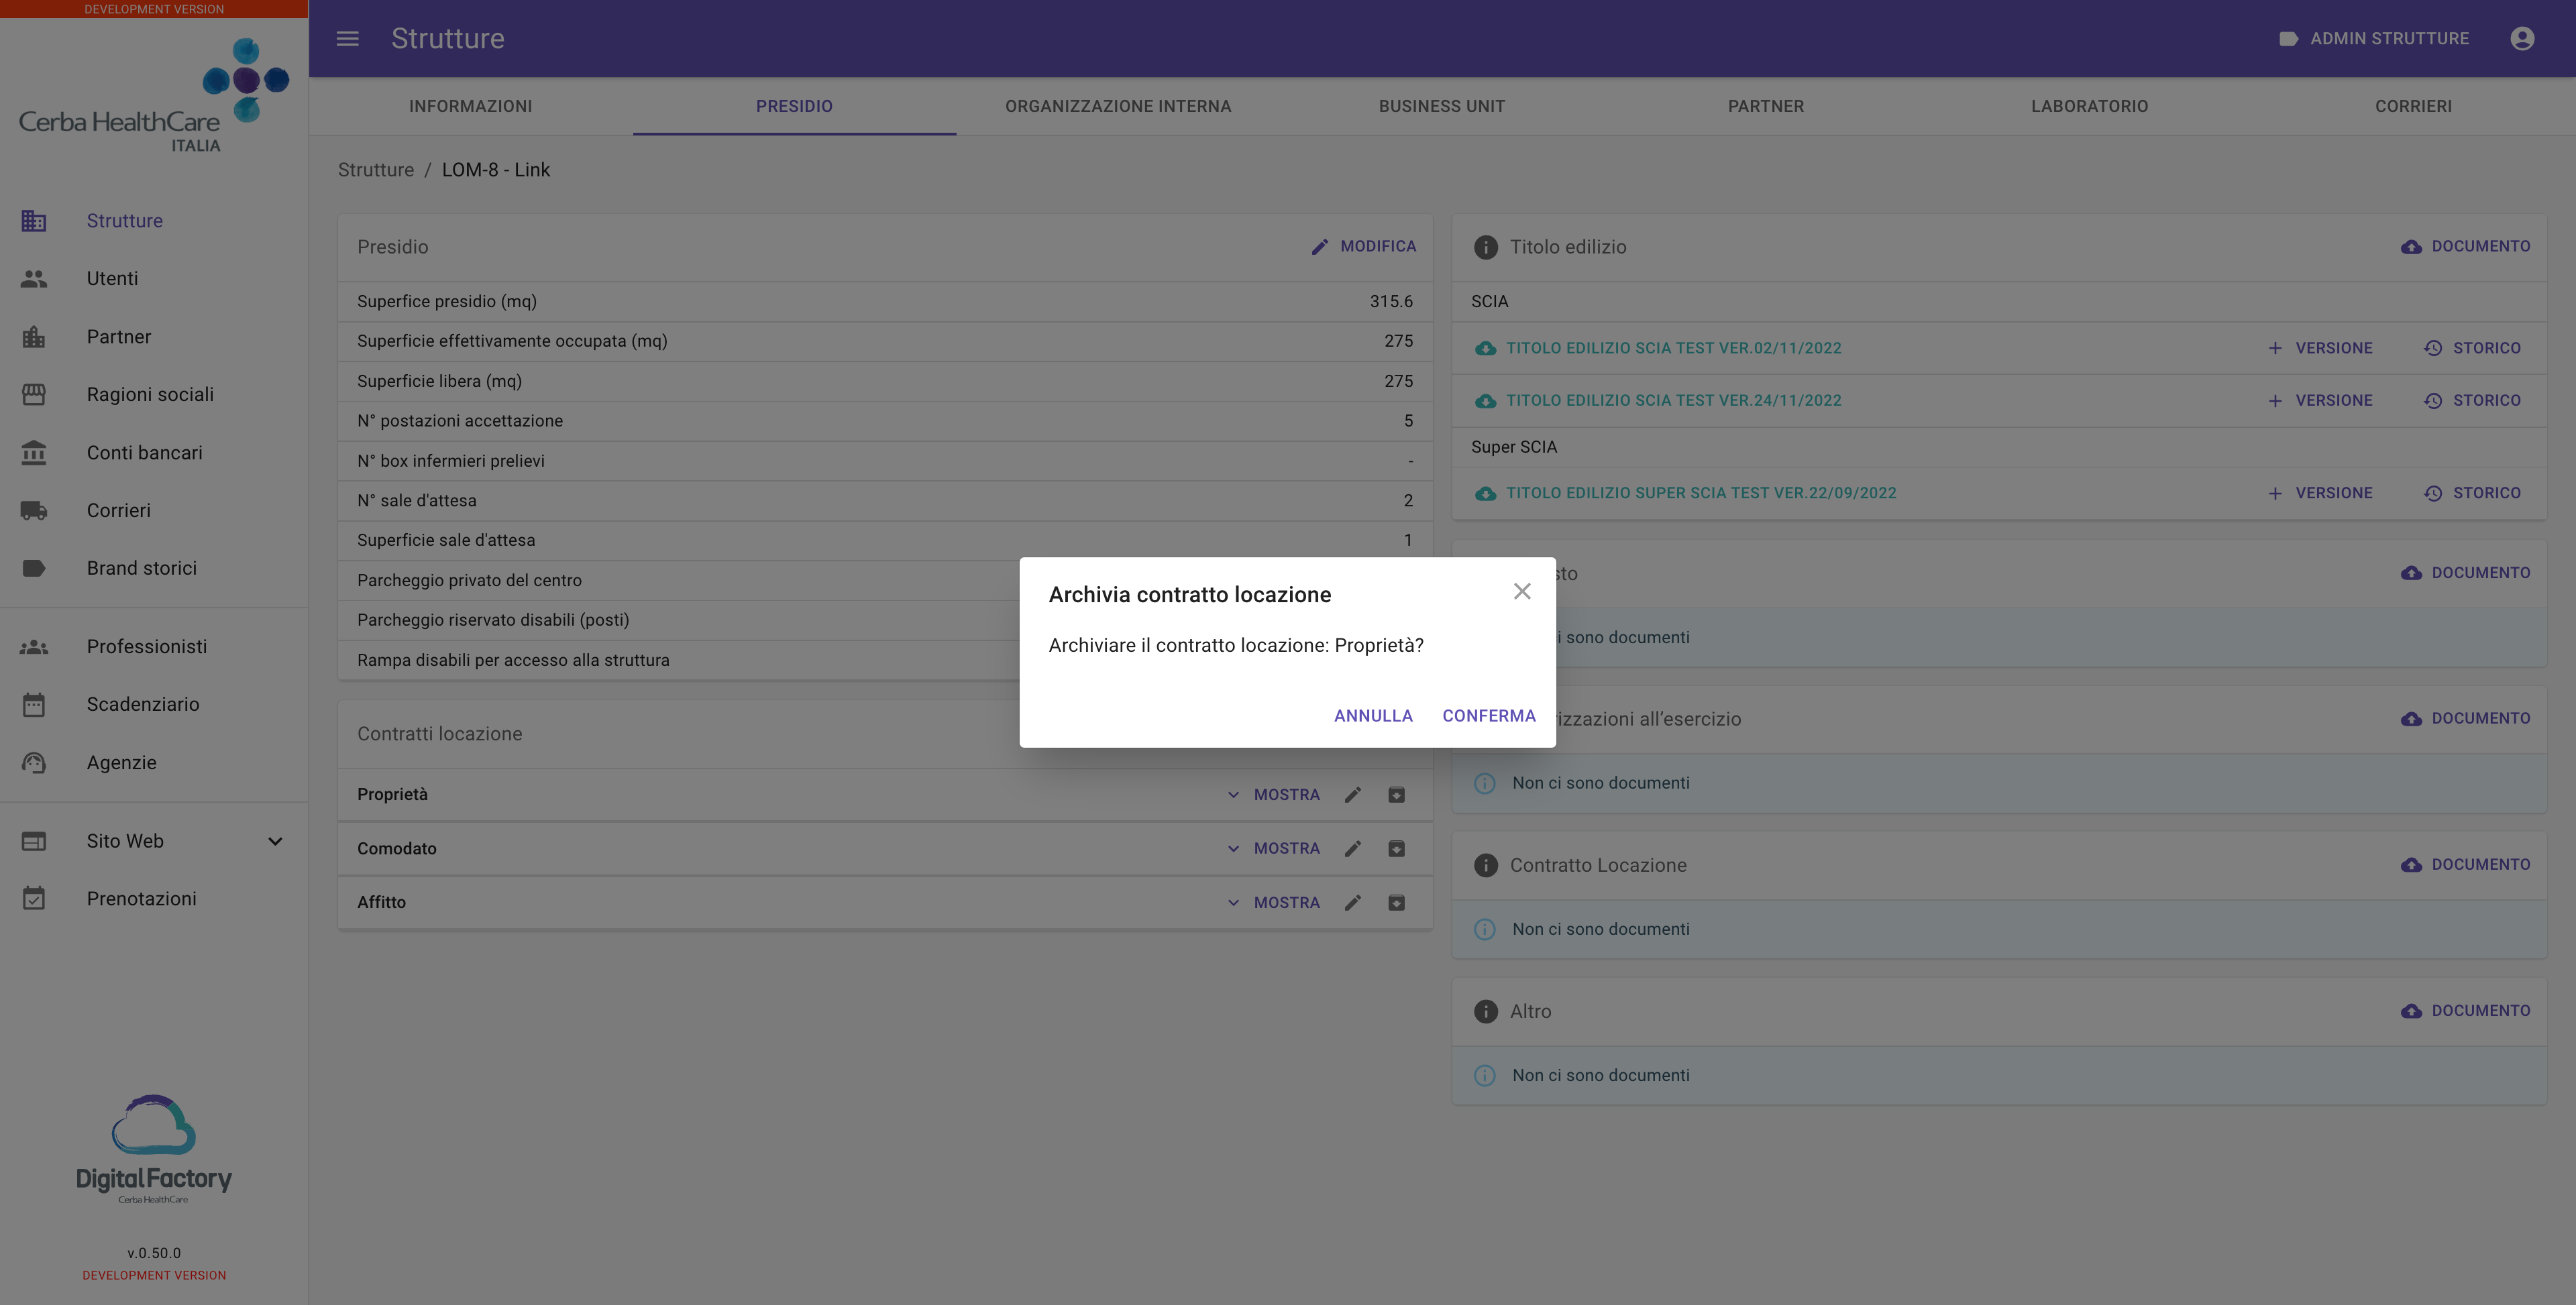
\includegraphics[width=0.75\textwidth]{images/capitolo5/f4_rentalAgreement/ModalRentalAgreement_archive.png} 
    \caption{Modale archiviazione contratto esistente} 
    \label{fig:ModalRentalAgreement_archive}
\end{figure}

\begin{figure}[H]
    \centering
    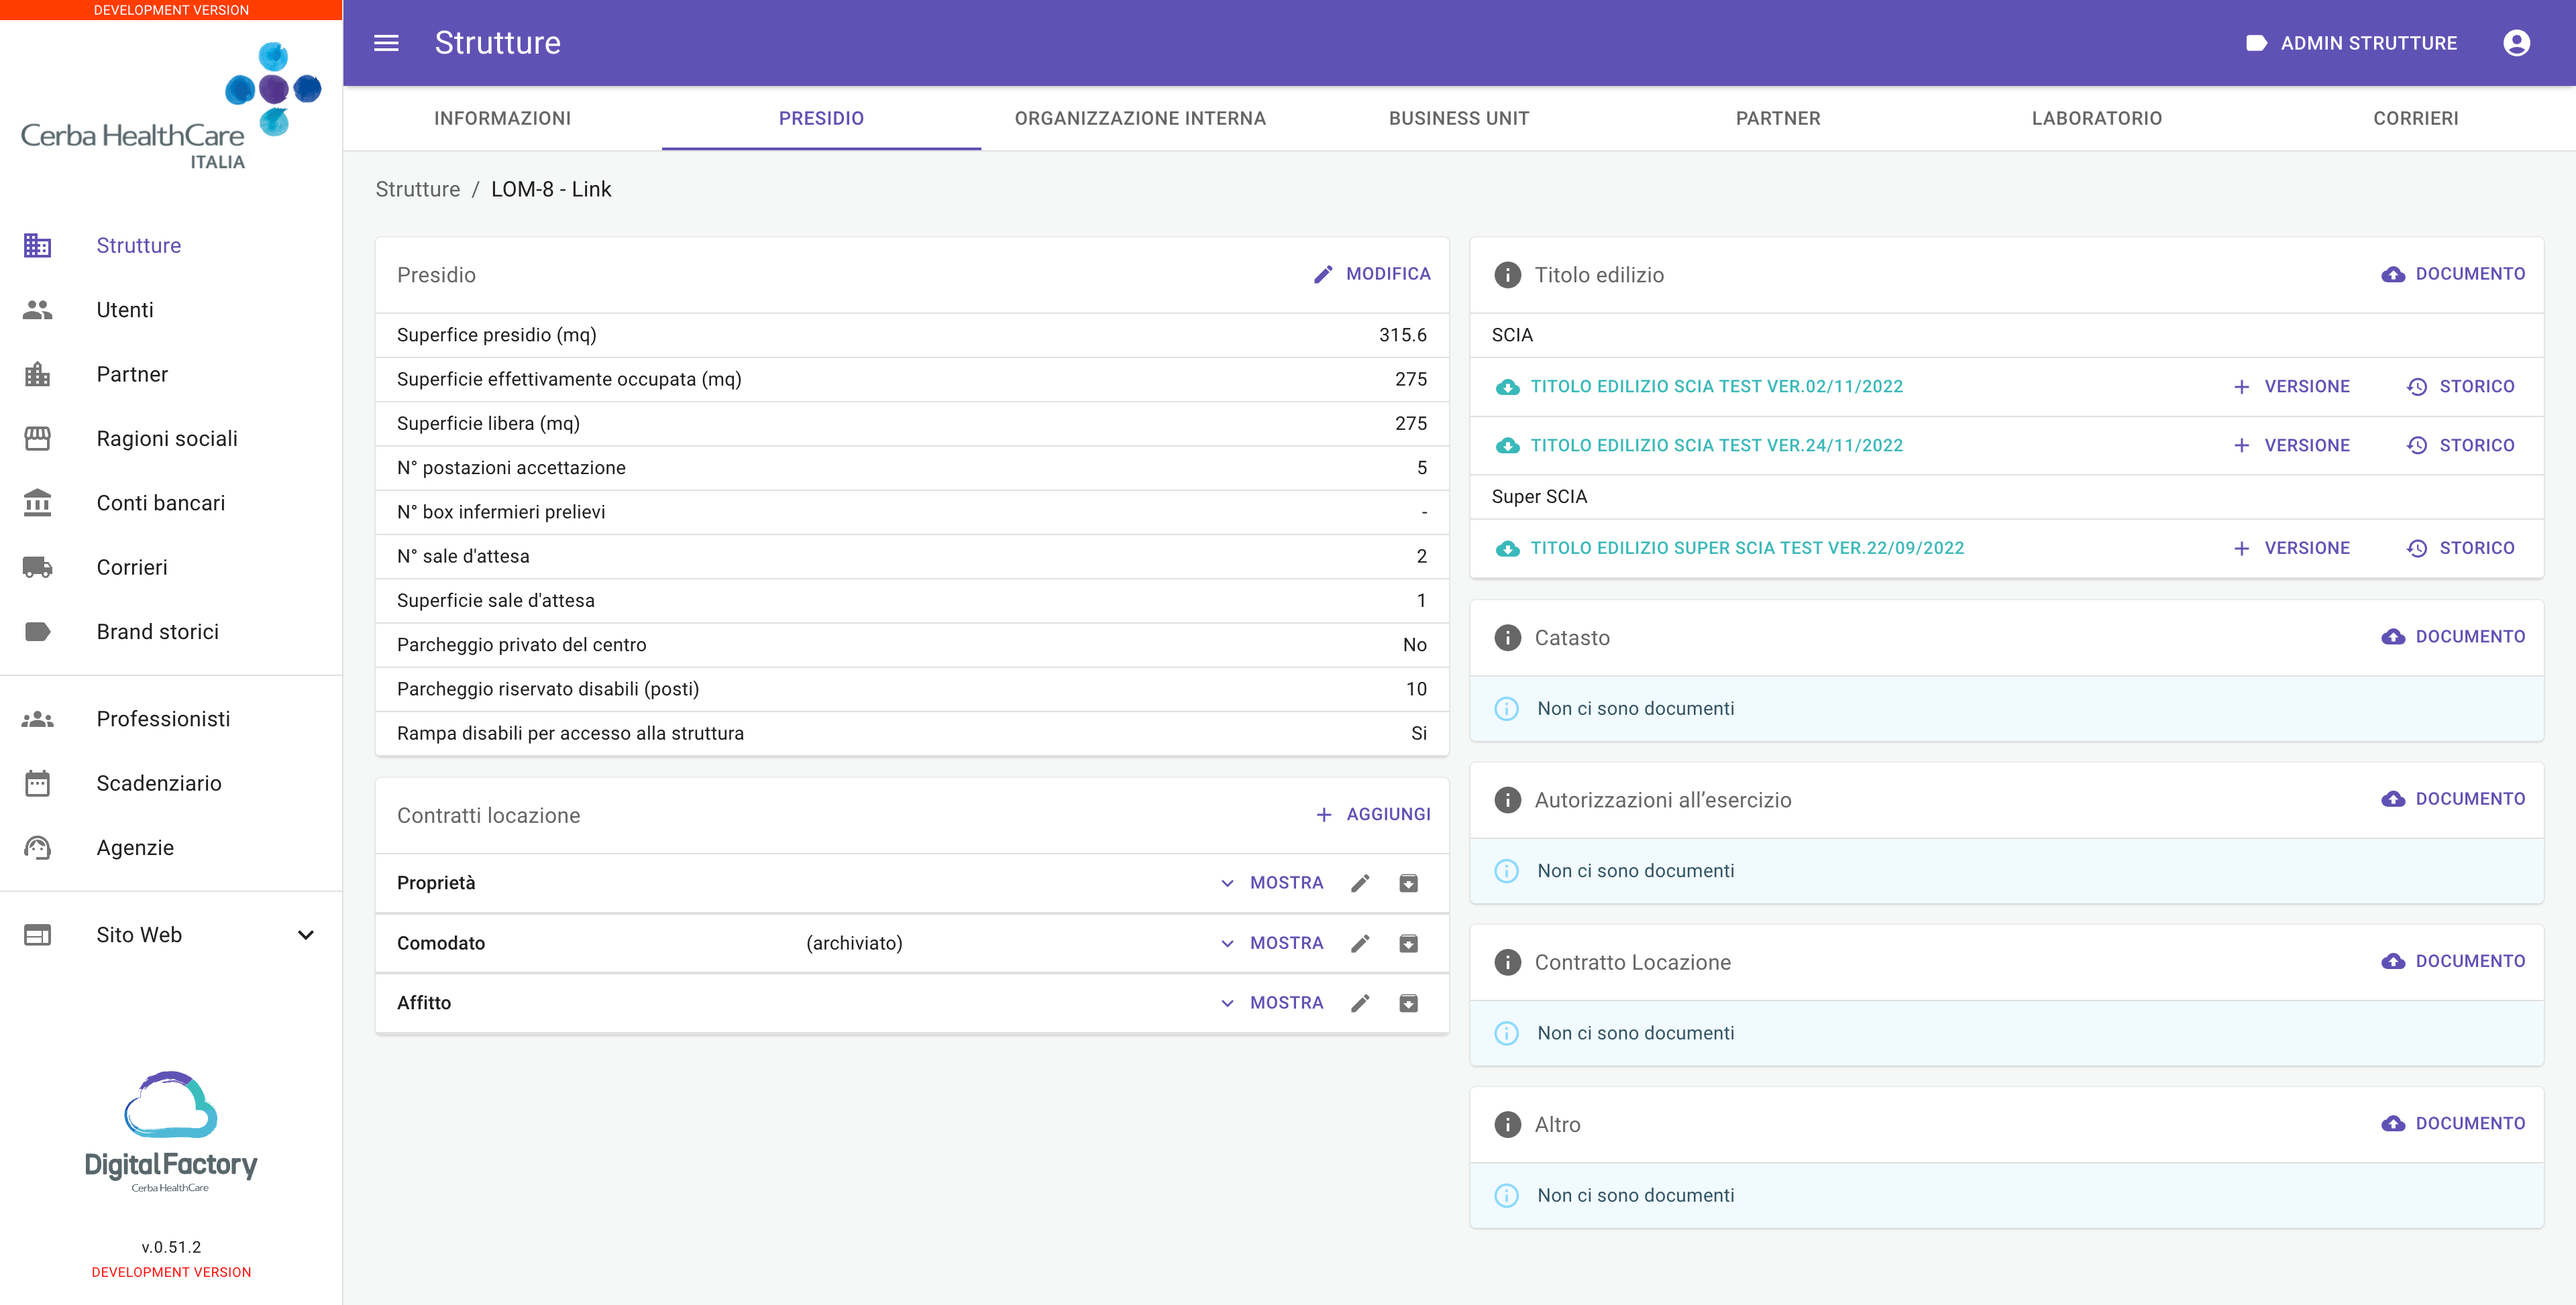
\includegraphics[width=0.75\textwidth]{images/capitolo5/f4_rentalAgreement/RentalAgreement_collapsed.png} 
    \caption{Tabella contratti non espansa} 
    \label{fig:RentalAgreement_collapsed}
\end{figure}

\begin{figure}[H]
    \centering
    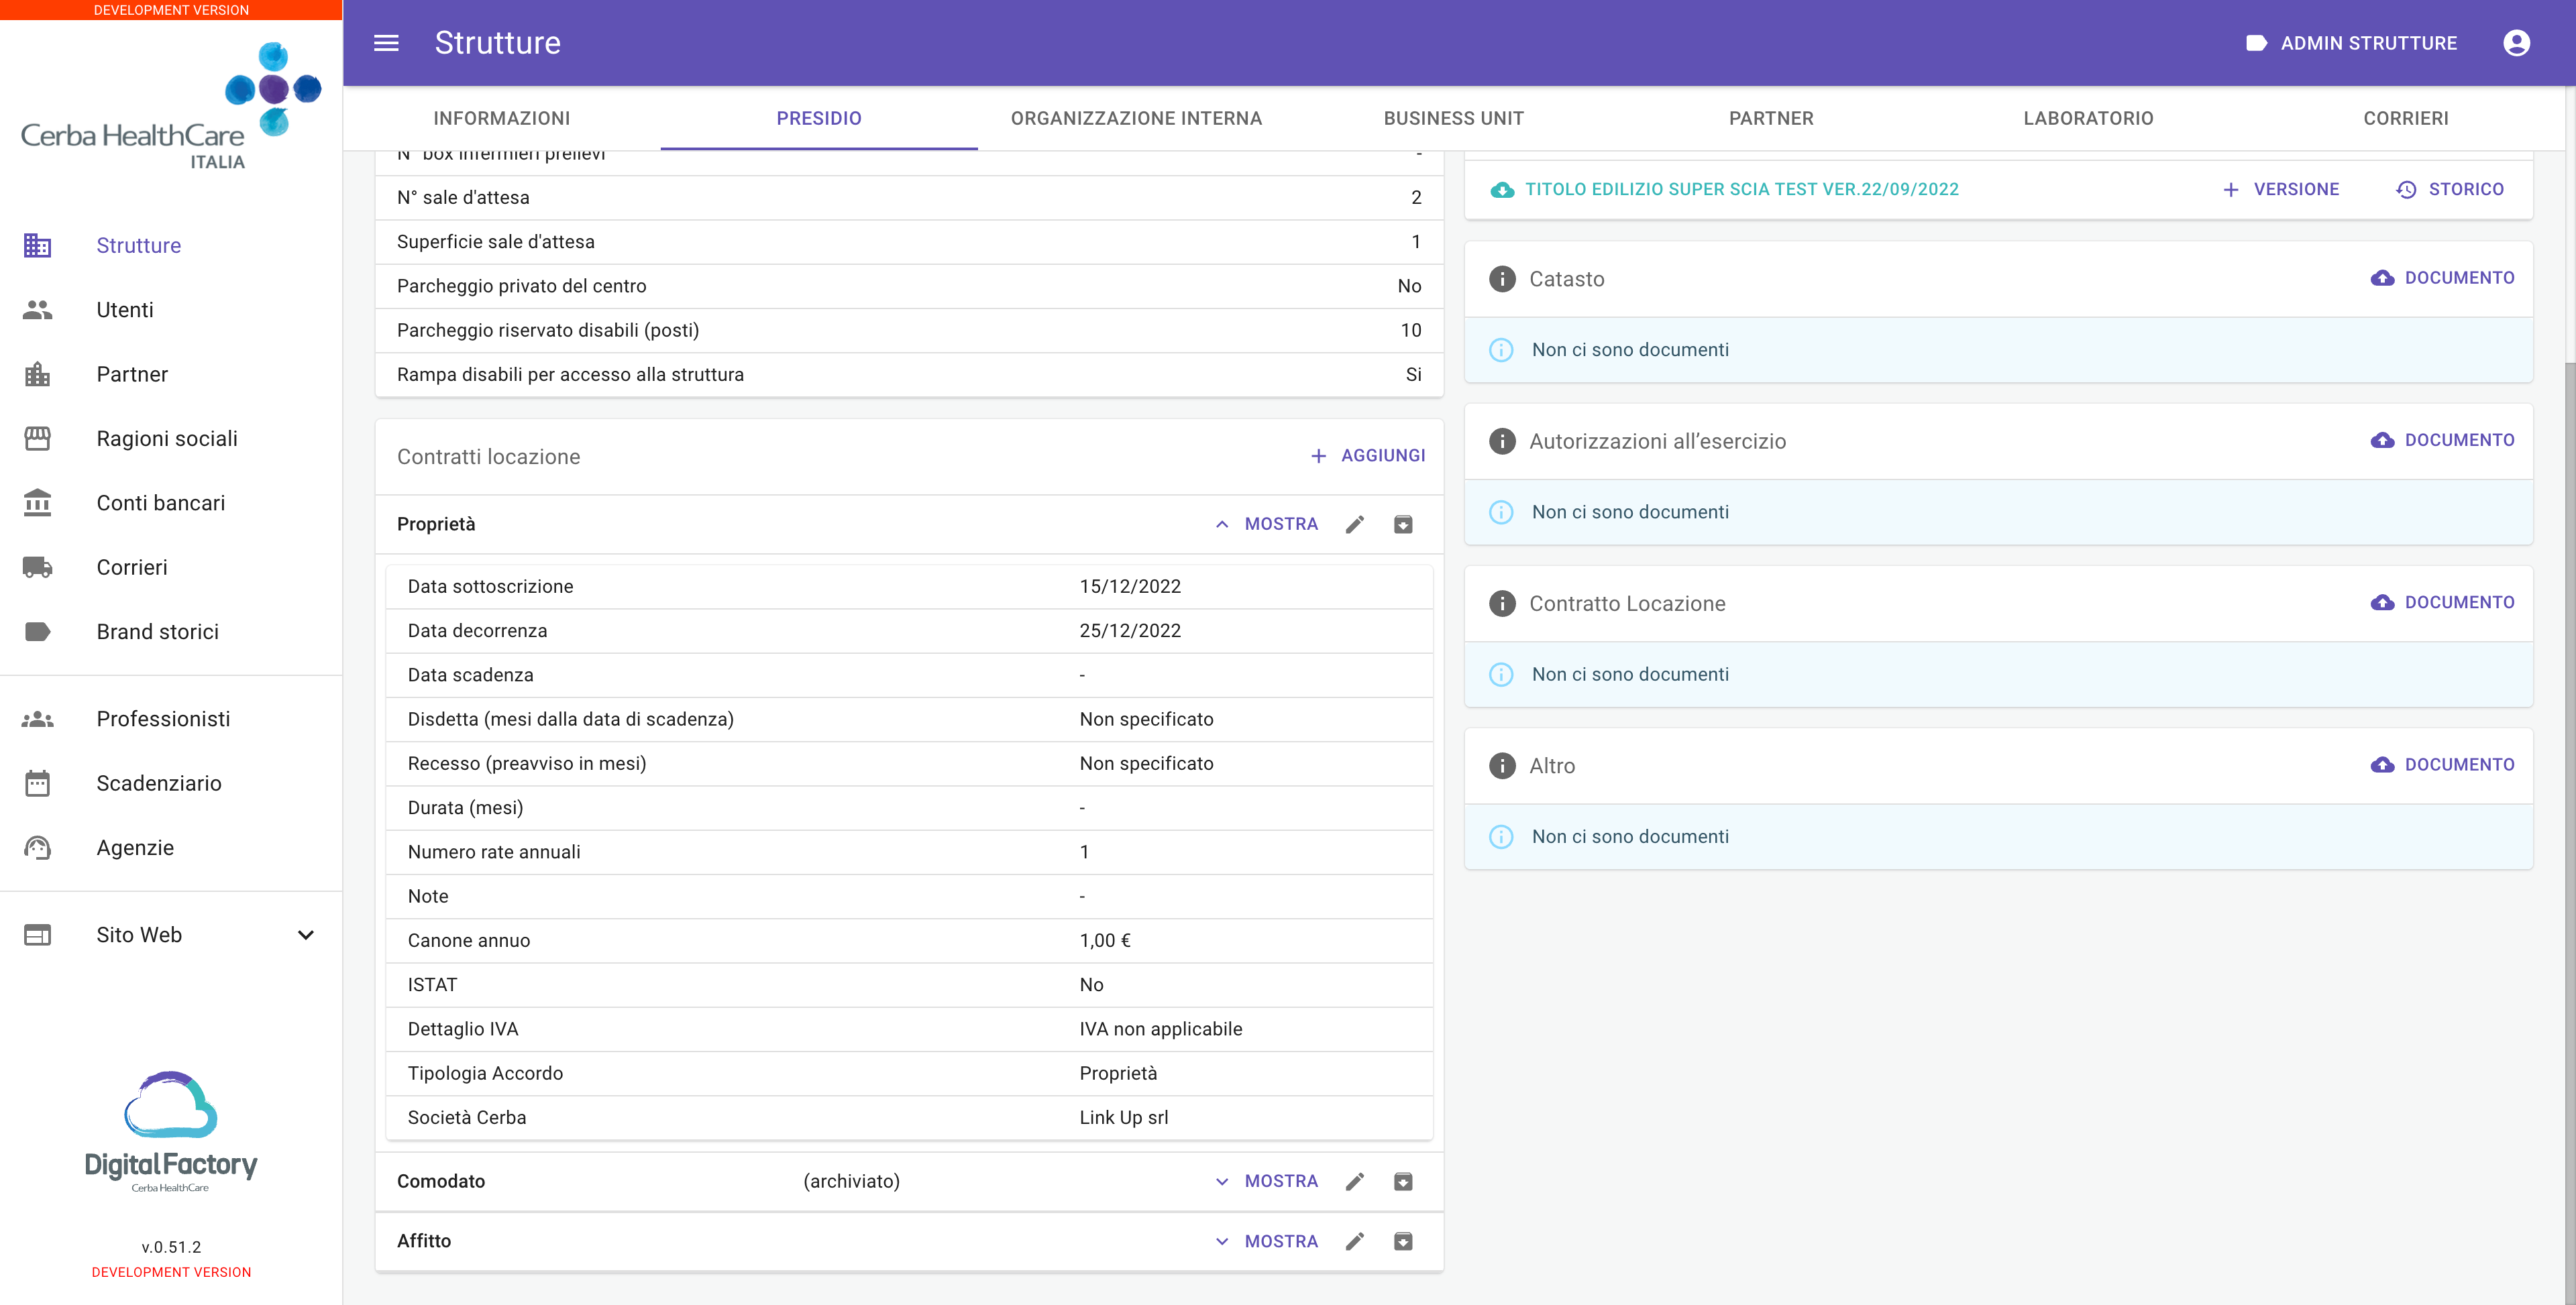
\includegraphics[width=0.75\textwidth]{images/capitolo5/f4_rentalAgreement/RentalAgreement_notCollapsed.png} 
    \caption{Tabella contratti con riga espansa} 
    \label{fig:RentalAgreement_notCollapsed}
\end{figure}

\newpage\section{F5: inserimento campo ricerca}
\label{sec:F5: inserimento campo ricerca}
La \textit{feature} F5 è stata caratterizzata da un certo livello di ridondanza: dopo la scrittura della nuova porzione di codice per la prima volta, l'implementazione è consistita semplicemente nella sua riproduzione dove previsto.\\
Nonostante piccole modifiche siano state operate di volta in volta ove necessario, i cambiamenti effettuati non rappresentano un qualcosa di così rilevante da giustificare  
l'inserimento dell'\textit{output} grafico di ogni situazione in cui l'implementazione è stata effettuata.

\subparagraph{Requisiti} 
L'\textit{header} della tabella di ognuna delle schede che formano la sezione “Ruoli Utente” (le schede sono: \textit{REO}, \textit{Area Manager}, \textit{Center Manager}, \textit{Data Manager}, \textit{Coordinatore Turni} e \textit{Coordinatore Compensi}) deve essere dotato di un campo di ricerca. Questo deve essere in grado di filtrare gli utenti per nome e/o cognome e posizionato alla sinistra del bottone per l'aggiunta di un ruolo utente.

\subparagraph{Procedura}
L'intero processo che ha portato all'implementazione del campo di ricerca all'interno della scheda del ruolo utente REO è avvenuto all'interno dello stesso componente, \texttt{TabReo}.

Il \textbf{primo \textit{step}} è consistito nella creazione della logica responsabile del suo funzionamento.\\
Ciò ha necessitato, \textit{in primis}, la dichiarazione della variabile di stato \texttt{filter} e del relativo \textit{setter} \texttt{setFilter()} attraverso l'\textit{hook} \texttt{useState()}. Tale variabile ha il compito di “memorizzare” il testo immesso, lato client, all'interno della casella di testo del campo di ricerca. Poiché, salvo introduzione di testo da parte dell'utente, il campo di ricerca si presenta come vuoto, la variabile \texttt{filter} è inizializzata con una stringa vuota \texttt{''}. Il contenuto di tale variabile viene aggiornato in continuazione con quanto scritto lato client attraverso il \textit{setter} \texttt{setFilter()}.

\lstinputlisting[caption=Variabile di stato \texttt{filter}, label=f5_TabReos_useState, language=JSX]{listings/capitolo5/f5_searchField/TabReos_useState.js}

In secondo luogo, è stata creata la variabile più propriamente responsabile del funzionamento della dinamica di ricerca, \texttt{filtered}. Questa implementa l'\textit{hook} \texttt{useMemo()} per il miglioramento delle \textit{performance} di esecuzione della ricerca.\\
All'interno del corpo di questa funzione è stata dichiarata la variabile \texttt{\_filter} (a riga 2): l'utilizzo dei metodi \texttt{toLowerCase()} e \texttt{trim()} sulla variabile di stato \texttt{filter}, assicura che il testo (in essa inserito ed immagazzionato) venga archiviato all'interno di un'altra variabile, \texttt{\_filter}, trasformato in minuscolo.\\
In seguito è stata dichiarata la variabile \texttt{filtered}: grazie allo \textit{spread operator} viene effettuata una copia di tutti i ruoli utente immagazzinati nella variabile \texttt{reos}\footnote{La variabile \texttt{reos}, assente nel \autoref{f5_TabReos_logic} perché già presente all'interno del codice, è frutto della chimata all'\gls{api} \texttt{getReos()}.}.\\
La condizione composta da un solo \texttt{if} ( da riga 6 a 12) costituisce la sezione più importante della variabile \texttt{filtered}; questa esprime il seguente concetto: se la lunghezza di \texttt{\_filter} è maggiore di \texttt{0}, sovrascrivi il precedente valore di \textit{filtered} con i soli utenti frutto del filtraggio, eseguito tramite l'iteratore \texttt{filter()}, sull'oggetto \texttt{filtered}.\\
Tale filtraggio, attraverso i metodi \texttt{toLowerCase()} e \texttt{includes()} sull'espressione che li precede, seleziona solo gli elementi (contenuti dalla variabile \texttt{filtered}) il cui nome e cognome o il cognome e nome in minuscolo include quando contenuto in \texttt{\_filter}.\\
In altre parole, vengono restituiti gli utenti del ruolo utente REO che corrispondono a quanto scritto all'interno del campo di ricerca.

\lstinputlisting[caption=Variabile \texttt{filtered}, label=f5_TabReos_UI, language=JSX]{listings/capitolo5/f5_searchField/TabReos_logic.js}

Il \textbf{secondo passaggio} è consistito nella creazione della porzione di interfaccia del campo di ricerca.\\
L' oggetto \texttt{table}\footnote{Il \textit{rendering} dell' oggetto \texttt{table} avviene grazie al componente \texttt{SuperTable} (all'interno del metodo \texttt{render()}). Per una speigazione più approfondita, si veda la \autoref{subsec:F6: “Magazine”}.} è stata modificata aggiungendo, all'interno della proprietà \texttt{action}, il componente \texttt{TextField}. Fra le molteplici \textit{props} di cui è dotato le più importanti sono:
\begin{itemize}
    \item \texttt{label}: il suo valore è la stringa \texttt{"Filtra per nome o cognome"};
    
    \item \texttt{placeholder}: il suo valore è la stringa \texttt{"Cerca"};
    
    \item \texttt{value}: il suo valore è la variabile di stato \texttt{filter};
    
    \item \texttt{onChange}: il suo valore è una funzione che permette di sostituire il contenuto della variabile di stato \texttt{filter} sfruttando il \textit{setter} \texttt{setFilter()}. Il nuovo contenuto sarà di volta in volta la proprietà \texttt{value} dell'oggetto \texttt{target} ( contenuto a sua volta dall'oggetto \texttt{e});
    
    \item \texttt{InputProps}: il suo valore è l'oggetto \texttt{endAdornment}, il quale contiene al suo interno i componenti \texttt{InputAdornment}, \texttt{IconButton} e \texttt{ClearButton}. Il componente \texttt{IconButton} è stato dotato della \textit{prop} \texttt{onClick} associata, di nuovo, al \textit{setter} \texttt{setFilter()}. In questo caso, però, il suo argomento è una stringa vuota \texttt{''} che serve per “azzerare” il valore della variabile \texttt{filter} ogni volta che viene effettuato click su quel bottone.
\end{itemize}

Infine, è stato modificato l'\textit{array} protagonista del \textit{mapping} utilizzato per popolare la proprietà \texttt{rows}, le righe, dell'oggetto \texttt{table}, della tabella.
La sostituzione del precedente con \texttt{filtered} fa in modo che, ogni qualvolta viene effettuata una ricerca scrivendo all'interno dell'apposito campo, vengano restituite, nella tabella dei REO, solamente le righe della  che corrispondono ai criteri specificati per il filtraggio.

\lstinputlisting[caption=Aggiornamento della variabile \texttt{table}, label=f5_TabReos_logic, language=JSX]{listings/capitolo5/f5_searchField/TabReos_UI.js}

\newpage\paragraph{\textit{Output} grafico}
\begin{figure}[H]
    \centering
    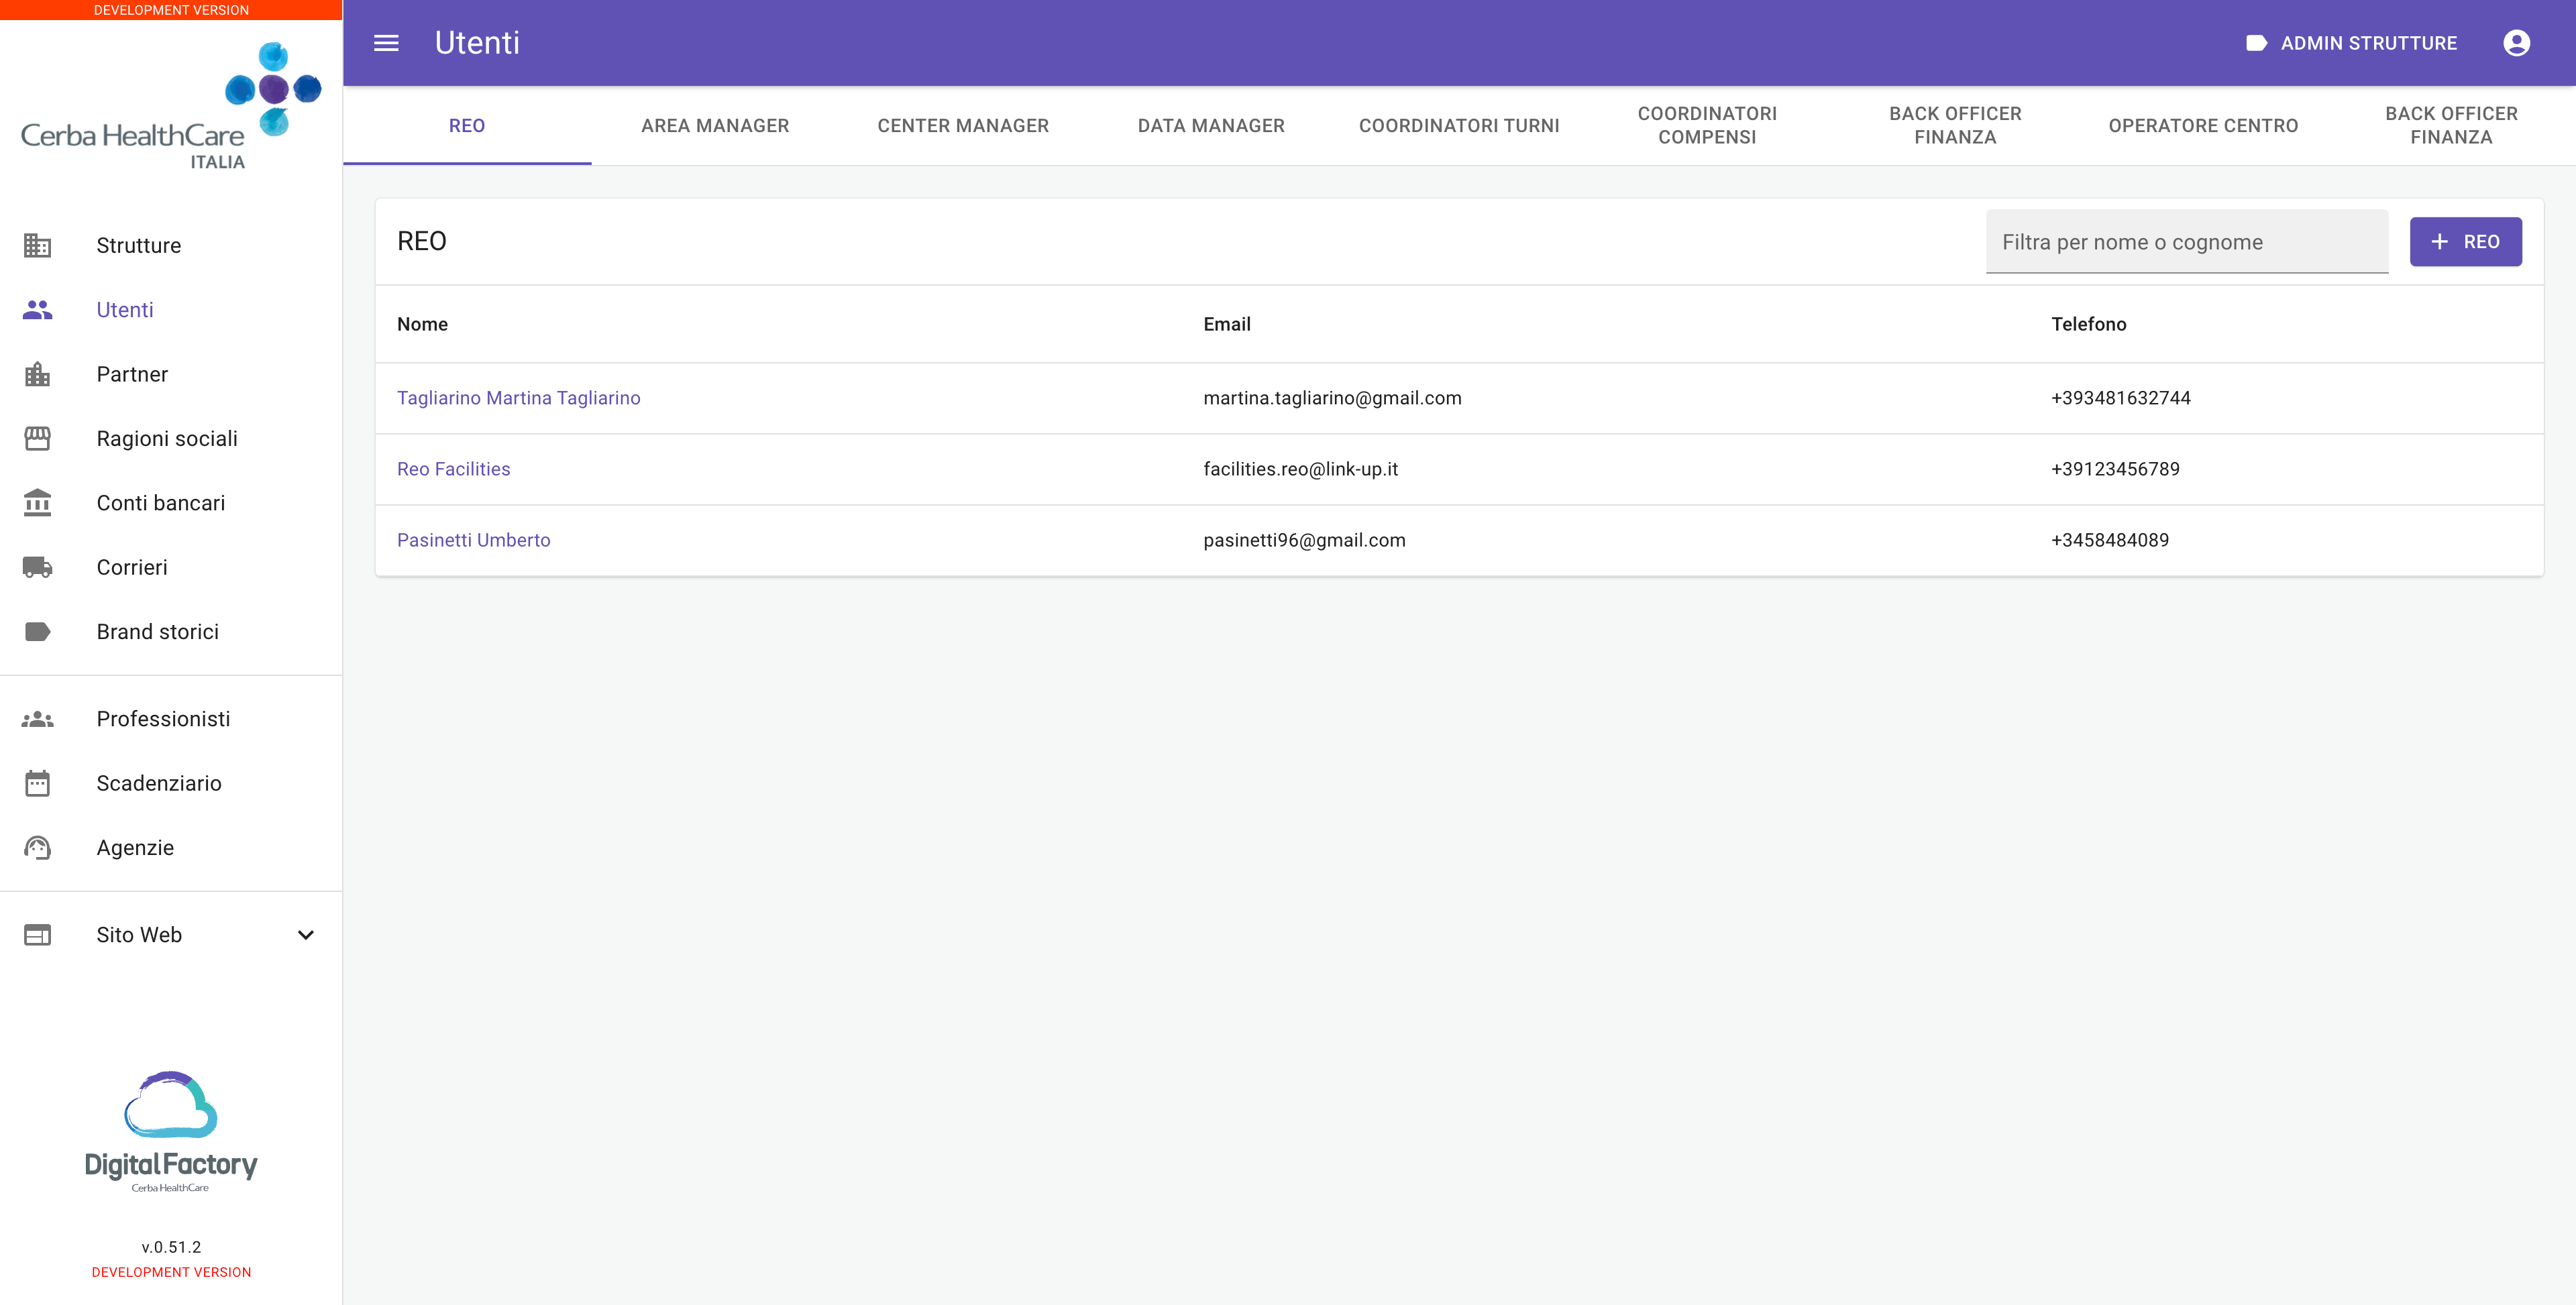
\includegraphics[width=0.75\textwidth]{images/capitolo5/f5_search/TabReo_searchEmpty.png} 
    \caption{Tabella REO campo ricerca vuoto} 
    \label{fig:TabReo_searchEmpty}
\end{figure}

\begin{figure}[H]
    \centering
    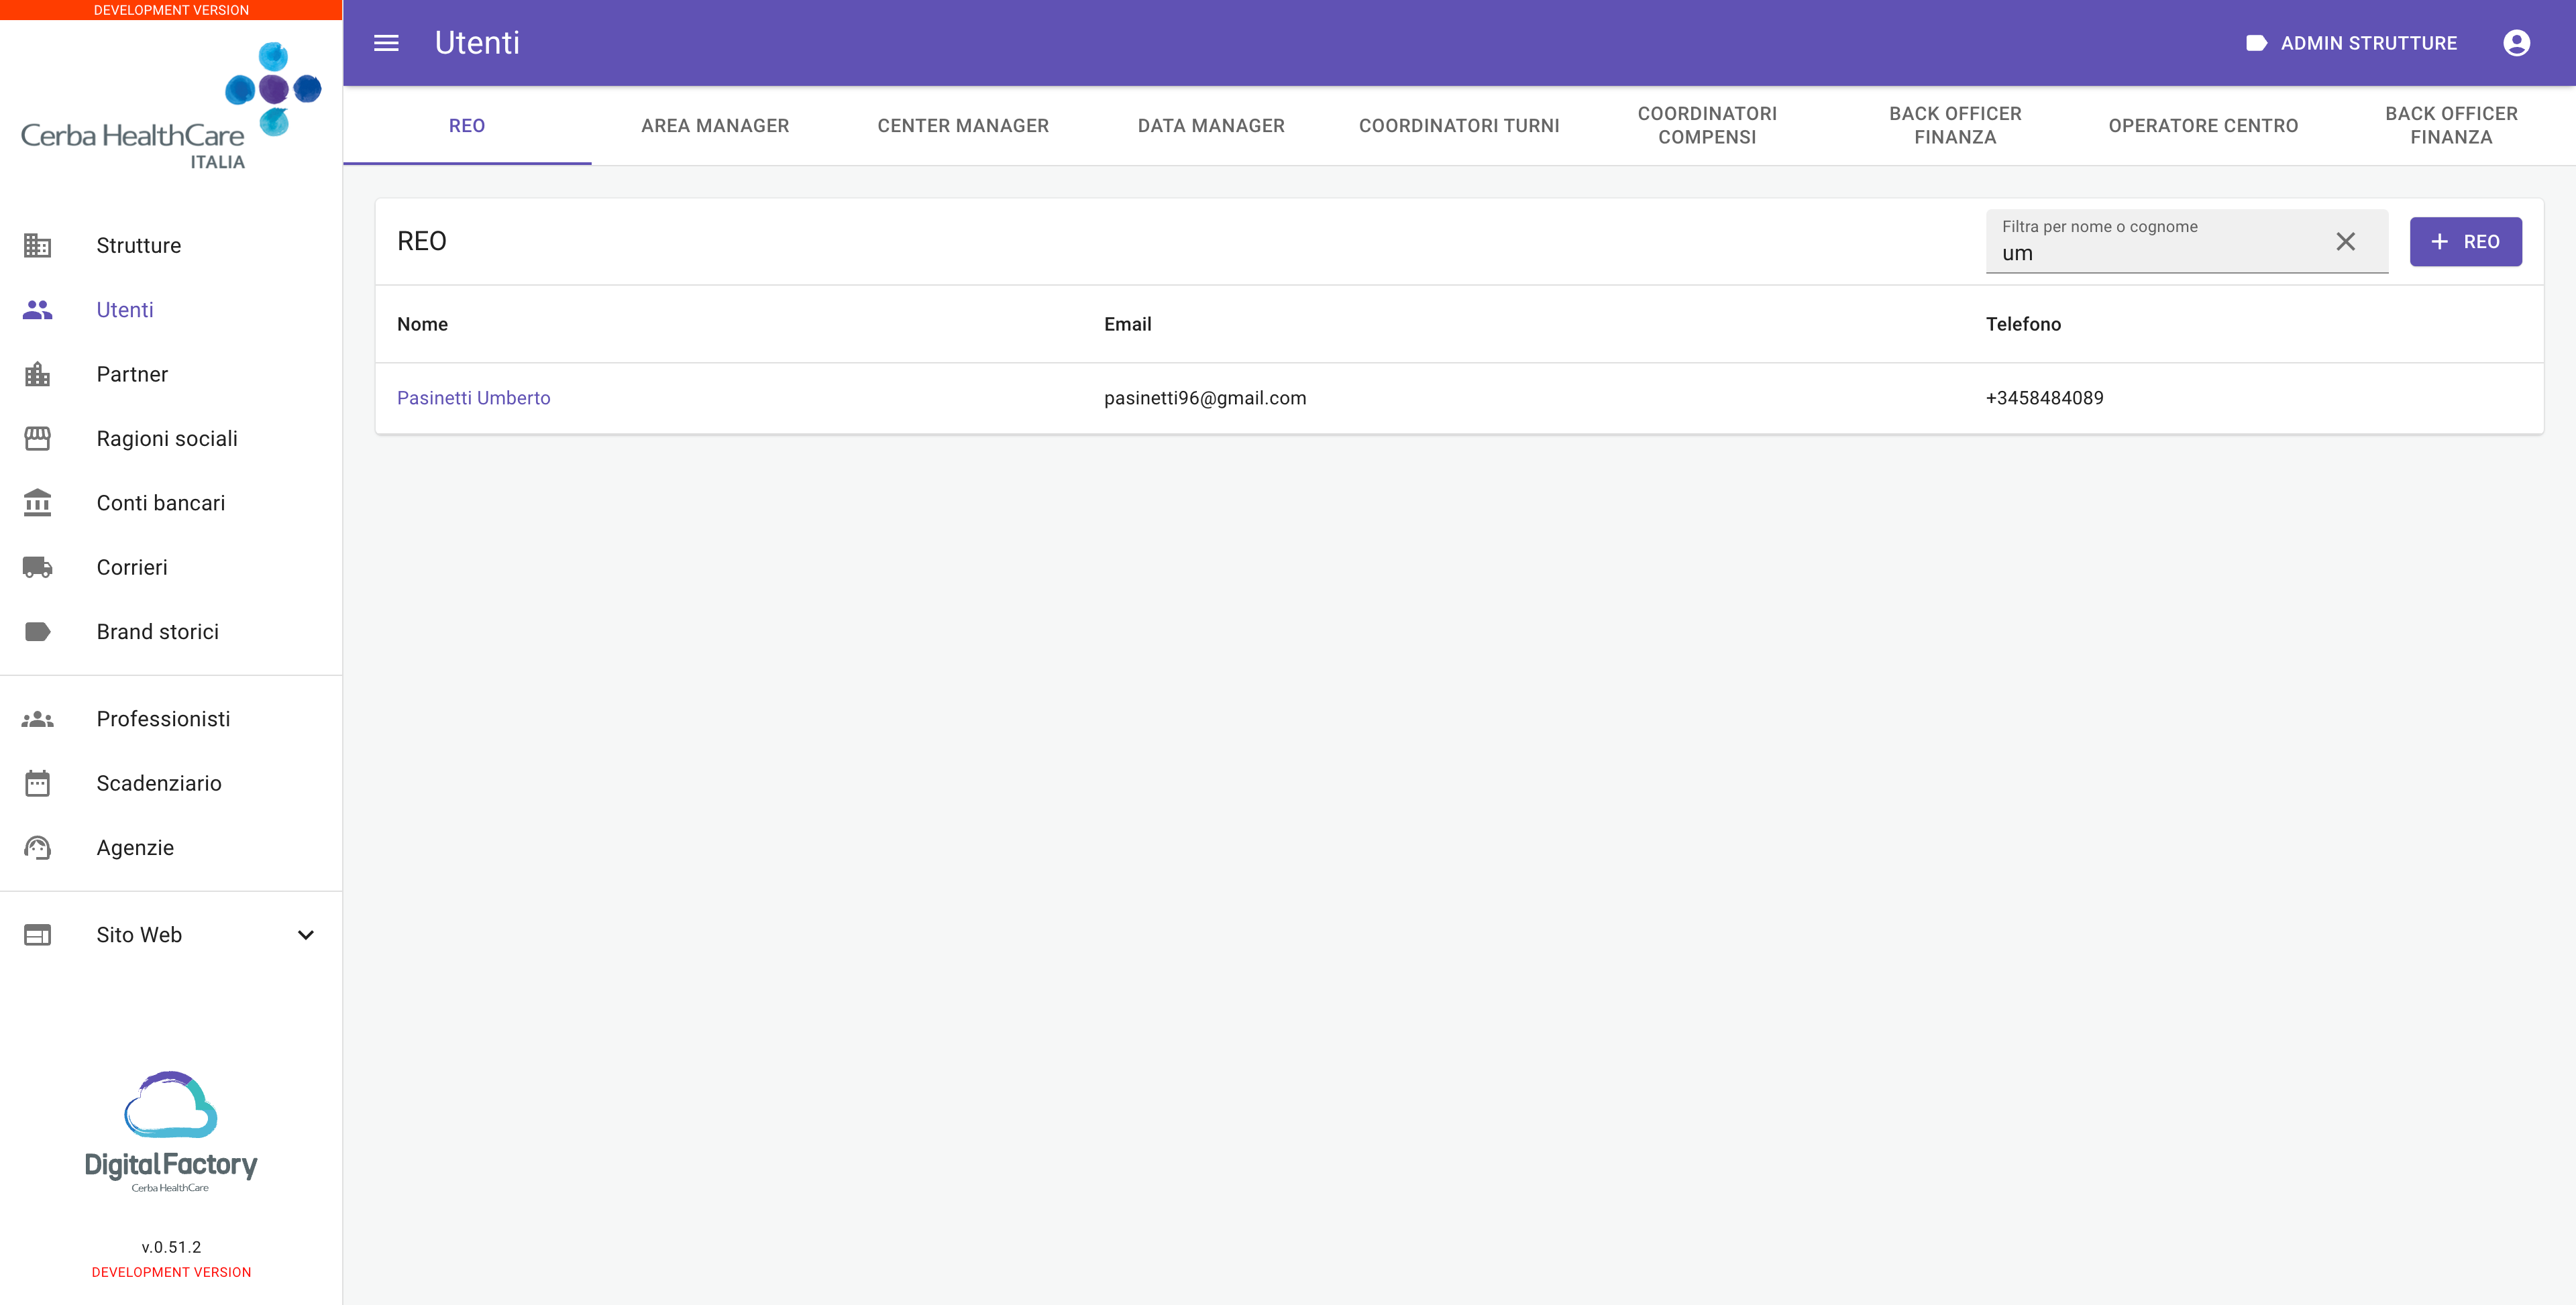
\includegraphics[width=0.75\textwidth]{images/capitolo5/f5_search/TabReo_searchFilled.png} 
    \caption{Tabella REO campo ricerca riempito} 
    \label{fig:TabReo_searchFilled}
\end{figure}

\newpage\section{F6 - F10: inserimento sezione}
Le \textit{feature} F6, F7, F8, F9 e F10 hanno previsto l'inserimento di una nuova sezione.\\
Da un lato, le sezioni di F6 e F7 sono state formate da una pagina per la visualizzazione dell'elenco degli elementi esistenti, e dalle modali per l'aggiunta, la modifica e l'eliminazione di un elemento. Nonostante dei cambiamenti siano stati effettuati ove necessario, le prime due \textit{feature} sono molto simili fra loro; per questo motivo si è optato di riportare solamente l'\textit{output} grafico relativo all'implementazione di F6.\\
Dall'altro, le sezioni di F8, F9 e F10 sono state composte da una pagina per la visualizzazione dell'elenco degli elementi, e da una pagina di dettaglio dedicata a ognuno di essi. A seconda dei casi, tramite le modali è possibile aggiungere, modificare o eliminare dati dell'elemento o l'elemento stesso. Anche qui le varie \textit{feature} non differiscono di molto, ma rispetto a quanto fatto per il precedente “gruppo” di implementazioni è stato riportato sia l'\textit{output} grafico di F8 che di F10.

\subsection{F6: “Magazine”}
\label{subsec:F6: “Magazine”}
\subparagraph{Requisiti}
Aggiungere la sezione “Magazine” fra quelle previste per il ruolo utente \textit{marketing admin}.\\
Al suo interno, una tabella deve mostrare i magazine esistenti in una lista semplice e riportarne le proprietà “Titolo”, “Descrizione”, “Data”, “Immagine” e “Documento”.\\
Deve essere possibile aggiungere o eliminare un magazine.\\
Deve essere possibile effettuare il download del documento.\\
Solamente per la proprietà “Descrizione” deve essere fornita la possibilità di formattazione.\\
L'\textit{header} della tabella dei magazine deve essere dotato di un campo di ricerca. Questo deve essere in grado di filtrare per titolo e posizionato alla sinistra del bottone per l'aggiunta di un nuovo magazine.

\subparagraph{Procedura}
Lo \textbf{\textit{step} iniziale} ha riguardato l'aggiornamento del \textit{routing}, operazione che ha comportato l'esecuzione di alcune modifiche all'interno del componente responsabile della navigazione fra le pagine visualizzate dal ruolo utente \textit{marketing admin}, ovvero \texttt{MarketingAdminRoutes}.\\
Come illustrato dal \autoref{f6_MarketingAdminRoutes}, il suo compito è sia il \textit{rendering} della \textit{dashboard}, ovvero del componente \texttt{DashboardMarketingAdmin}, che il contenimento dei vari componenti che definiscono il percorso che l'utente può seguire muovendosi nella piattaforma. La modifica al \textit{routing} ha necessitato l'inserimento, all'interno del componente padre \texttt{Switch} (da riga 3 a 9), di un nuovo componente figlio \texttt{Route}, il quale racchiude a sua volta \texttt{PageMagazines}, l'istanza del nuovo componente che verrà restituito cliccando sul link della sezione “Magazines”. L'istanza di \texttt{PageMagazines} è dotata della \textit{prop} \texttt{path}, il cui valore è la stringa \texttt{"/magazine"}.\\
In altre parole, la navigazione può ora avvenire, oltre che fra le vecchie pagine (o meglio, fra i vecchi componenti), anche su \texttt{PageMagazines}.

\lstinputlisting[caption=\textit{Routing} di \texttt{PageMagazines}, label=f6_MarketingAdminRoutes, language=JSX]{listings/capitolo5/f6_magazines/MarketingAdminRoutes.js}

Il \textbf{secondo passo} è consistito nell'aggiornamento della \textit{dashboard}, il “pannello” di controllo del ruolo utente \textit{marketing admin}; ciò ha richiesto dei ritocchi al componente \texttt{DashBoardMarketingAdmin}.\\ 
Per prima cosa, come possibile vedere nel \autoref{f6_DashboardMarketingAdmin_titles}, l'oggetto che contiene i titoli dell'\textit{header} della \textit{dashboard}, \texttt{titles}, è stato dotato della proprietà \texttt{'/magazine'}. La stringa \texttt{'Magazine'}, il suo valore, diverrà il titolo della sezione “Magazine”.

\lstinputlisting[caption=Aggiornamento variabile \texttt{titles}, label=f6_DashboardMarketingAdmin_titles, language=JSX]{listings/capitolo5/f6_magazines/DashboardMarketingAdmin_titles.js}
% spazio
In secondo luogo, come mostrato del \autoref{f6_DashboardMarketingAdmin_sidebar}, si è intervenuto sulla variabile che contiene la lista dei componenti che formano il menu laterale, \texttt{sidebar}, alla quale è stato aggiunto quello relativo alla sezione “Magazine”. Le \textit{props} del nuovo elemento \texttt{Sidebar} appena introdotto sono:
\begin{itemize}
    \item \texttt{label}: stabilisce il testo dell'etichetta della sezione nel menu laterale, il suo valore è la stringa \texttt{'Magazine'};
    
    \item \texttt{href}: stabilisce il percorso da seguire per visualizzare il componente, il suo valore è la stringa \texttt{'/magazine'};
    
    \item \texttt{icon}: stabilisce l'immagine da visualizzare accanto all'etichetta, il suo valore è il componente \texttt{NewspaperIcon}.
    
    % \item \texttt{isActive}: il suo valore è la funzione \texttt{isActive()};
\end{itemize}

\lstinputlisting[caption=Aggiornamento variabile \texttt{sidebar}, label=f6_DashboardMarketingAdmin_sidebar, language=JSX]{listings/capitolo5/f6_magazines/DashboardMarketingAdmin_sidebar.js}

Il \textbf{terzo passo} ha avuto a che fare con la creazione delle funzioni \texttt{getMagazines()}, \\\texttt{createMagazine()} e \texttt{deleteMagazine()}, le funzioni che effettuano le chiamate alle \gls{api} visibili nel \autoref{f6_api}. All'interno del loro corpo (alle righe righe 1, 4 e 7) sono state utilizzate, rispettivamente, le funzioni \texttt{get()}, \texttt{post()} e \texttt{del()}, funzioni che hanno il compito di effettuare le richieste avvalendosi dei metodi \texttt{GET}, \texttt{POST} e \texttt{DELETE}.

\lstinputlisting[caption=Funzioni di chiamata alle \gls{api} per la sezione “Magazine”, label=f6_api, language=JSX]{listings/capitolo5/f6_magazines/api.js}

Il \textbf{quarto} e \textbf{ultimo passo}, il più complesso e lungo, ha riguardato la modellazione dei componenti che formano la sezione “Magazine” e con i quali è possibile interagire.

% ! PageMagazine
\texttt{PageMagazines}, il primo realizzato (la cui istanza è stata vista nel \textit{routing} del ruolo utente \textit{marketing admin}), è illustrato nel \autoref{f6_PageMagazines_component} ed ha lo scopo di effettuare il \textit{rendering} della tabella che contiene la lista dei magazine.

\lstinputlisting[caption=Componente \texttt{PageMagazines}, label=f6_PageMagazines_component, language=JSX]{listings/capitolo5/f6_magazines/PageMagazines_component.js}
% spazio
Innanzitutto, al componente è stata fornita la logica necessaria per il suo funzionamento.\\
Come mostrato dal \autoref{f6_PageMagazines_get}, la funzione \texttt{getMagazines()} è passata come argomento all'\textit{hook} \texttt{useApi()} per reperire i magazine da visualizzare, \texttt{magazines}, le informazioni relative al caricamento e all'errore, \texttt{isLoading} ed \texttt{error}, e la funzione che permette di aggiornare la lista dei magazine, \texttt{fetchMagazines}.

\lstinputlisting[caption=Utilizzo \texttt{getMagazines()}, label=f6_PageMagazines_get, language=JSX]{listings/capitolo5/f6_magazines/PageMagazines_get.js}
% spazio
I due \textit{handler} dichiarati in \texttt{PageMagazines} sono \texttt{handleDeleteMagazine()} e \\\texttt{handleConfirmDeleteMagazine}. Come mostrato nel \autoref{f6_PageMagazines_handlers}, se da un lato, il primo è noto per struttura e scopo poiché già incontrato nella \autoref{sec:F4: modifica tabella contratti di locazione}, dall'altro, il secondo costituisce un qualcosa di completamente nuovo.\\
La funzione \texttt{handleDeleteMagazine}, infatti, appartiene a quel gruppo di \textit{handler} che hanno il compito di aprire una modale, e le operazioni che esegue sono: 
\begin{enumerate}
    \item L'impostazione, tramite il \textit{setter} \texttt{setData()}, dei dati della modale \\\texttt{modalConfirmDeleteMagazine}, sull'oggetto \texttt{magazine};
    
    \item L'apertura della modale tramite la funzione \texttt{open()}.
\end{enumerate}
Gli oggetti relativi alla modale \texttt{modalConfirmDeleteMagazine} e \texttt{modalMagazine} sono stati dichiarati attraverso il \textit{custom hook} \texttt{useModal()} (alle righe riga 1 e 3); \texttt{modalMagazine} è utilizzata per l'aggiunta di nuovi magazine.\\
L'\textit{handler} \texttt{handleConfirmDeleteMagazine}, invece, è una funzione atta all'effettiva manipolazione dei dati, e le operazioni che esegue sono: 
\begin{enumerate}
    \item L'eliminazione, dal \textit{bucket} \texttt{marketing}, della proprietà \texttt{path} dell'oggetto \texttt{0} all'interno dell'\textit{array} \texttt{files} (contenuto a sua volta, a risalire, dagli oggetti \texttt{document}, \texttt{magazine}, \texttt{data} e \texttt{modalConfirmDeleteMagazine}), con l'invocazione della funzione \texttt{removeToS3()};
    
    \item L'eliminazione, dal \textit{bucket} \texttt{marketing}, della proprietà \texttt{path} contenuta dall'oggetto \texttt{image} (contenuta a sua volta, a risalire, da \texttt{magazine}, \texttt{data} e \texttt{modalConfirmDeleteMagazine}), con l'invocazione della funzione \texttt{removeToS3()};
    
    \item L'effettiva eliminazione del magazine, con l'invocazione della funzione \texttt{deleteMagazine()}, alla quale viene passato come argomento l'\texttt{uuid} dell'oggetto \texttt{magazine} (contenuto a sua volta, a risalire, dagli oggetti \texttt{data} e \texttt{modalConfirmDeleteMagazine});
    
    \item L'aggiornamento della lista dei magazine, con l'invocazione della funzione \texttt{fetchMagazines()}.
\end{enumerate}

\lstinputlisting[caption=\textit{Handler} componente \texttt{PageMagazines}, label=f6_PageMagazines_handlers, language=JSX]{listings/capitolo5/f6_magazines/PageMagazines_handlers.js}
% spazio
\texttt{PageMagazines} contiene poi la logica relativa al campo di ricerca. Il suo funzionamento è sostanzialmente identico a quello visto nella \autoref{sec:F5: inserimento campo ricerca}, ma la sua struttura si differenzia parzialmente da quella della \textit{feature} F5.\\
La dinamica di filtraggio è qui inserita all'interno dell'\textit{hook} \texttt{useEffect()}; inoltre, la condizione \texttt{if} (a riga 9) si caratterizza per il fatto che il valore/i restituito dal filtraggio\footnote{Il valore restituito dal filtraggio è assegnato alla variabile \texttt{\_filtered}.}, effettuato nuovamente tramite l'iteratore \texttt{filter()}, corrisponde all'elemento/i, all'interno dei magazine, il cui titolo in minuscolo corrisponde a quando presente nella variabile \texttt{\_filterName}. 

\lstinputlisting[caption=Dinamica di filtraggio della sezione magazine, label=f6_PageMagazines_search, language=JSX]{listings/capitolo5/f6_magazines/PageMagazines_search.js}
% spazio
La logica del primo componente creato si è conclusa specificando la posizione del \textit{bucket} in cui sono contenute le immagini associate ai magazine. Ciò è stato fatto grazie alla funzione \texttt{configure()} (invocata sull'oggetto \texttt{Amplify}), alla quale è passato come argomento un oggetto la cui unica proprietà, \texttt{Storage}, ha per valore l'ubicazione, ovvero la proprietà \texttt{marketing} di \texttt{storage} (contenuta, a risalire, dagli oggetti \texttt{amplify} e \texttt{config}). 

\lstinputlisting[caption=Configurazione di \texttt{Amplify}, label=f6_PageMagazines_amplifyConfigure, language=JSX]{listings/capitolo5/f6_magazines/PageMagazines_amplifyConfigure.js}
% spazio
Dopodiché, è stata modellata la \acrshort{ui} di \texttt{PageMagazines}. Il \textit{rendering} di questo componente avviene in modo particolare: all'interno della sua logica, è dichiarato un oggetto, \texttt{table}, che specifica tutte le caratteristiche della tabella da visualizzare, e che viene passato, sotto forma di \textit{prop}, a un componente, \texttt{SuperTable}, che “impagina” \texttt{table} ritornando a schermo la tabella dei magazine.\\
Per questo motivo, la gestione della veste grafica di \texttt{PageMagazines} è consistita principalmente nella manipolazione dell'oggetto \texttt{table}\footnote{L'oggetto \texttt{table} deve essere costruito necessariamente includendo proprietà che possono essere accettate dal componente \texttt{SuperTable}.}, le cui proprietà sono:
\begin{itemize}
    \item \texttt{title} (a riga 2): specifica il titolo della tabella, il suo valore è la stringa \texttt{'Magazine'};
    
    \item \texttt{noResults} (a riga 2): specifica il messaggio da restituire se la tabella è vuota, il suo valore è la stringa \texttt{'Nessun magazine trovato'};
    
    \item \texttt{action} (da riga 3 a 31): specifica le azioni che possono essere compiute nell'\textit{header} della tabella, il suo valore è un'espressione che permette di effettuare:
        \begin{itemize}
            \item La ricerca di un magazine fra quelli esistenti grazie al componente \texttt{TextField} (da riga 5 a 22). Le molteplici \textit{props} di cui è dotato sono sostanzialmente identiche a quelle descritte in relazione al medesimo componente nella \textit{feature} F5\footnote{Si veda la \autoref{sec:F5: inserimento campo ricerca}.};
            
            \item L'aggiunta di un nuovo magazine grazie al componente \texttt{Button} (da riga 24 a 29). Il testo restituito dal componente è “Magazine” e le sue più importanti \textit{props} sono:
            \begin{itemize}
                \item \texttt{onClick} (a riga 25): il suo valore è la funzione \texttt{open()} invocata sull'oggetto \texttt{modalMagazine};
                
                \item \texttt{startIcon} (a riga 26): il suo valore è il componente \texttt{AddIcon};
            \end{itemize}
        \end{itemize}
    
    \item \texttt{isLoading} e \texttt{error} (a riga 32): specificano delle informazioni relative allo stato di una chiamata ad un'\gls{api};
     
    \item \texttt{filter} (a riga 32): specifica il messaggio da ritornare sotto l'\textit{header} della tabella una volta eseguita una ricerca;
    
    \item \texttt{perPage} (a riga 32): specifica il numero di elementi da visualizzare in una pagina, il suo valore è \texttt{10};
    
    \item \texttt{headers} (da riga 33 a 40): specifica i titoli delle colonna della tabella, il suo valore è un'oggetto che, a sua volta, include gli oggetti \texttt{title}, \texttt{description}, \texttt{date}, \texttt{image}, \texttt{document} e \texttt{delete}. All'interno di ognuno di essi sono definite le caratteristiche del titolo stesso attraverso le proprietà:
        \begin{itemize}
            \item \texttt{label}: stabilisce il testo del titolo di una colonna, il suo valore è una stringa, ad esempio, \texttt{'Titolo'};
            
            \item \texttt{sort}: stabilisce se è possibile effettuare l'ordinamento dei magazine in base alla proprietà della colonna in considerazione, il suo valore è un valore booleano, ad esempio, \texttt{true};
            
            \item \texttt{width}: stabilisce la larghezza della colonna, il suo valore è un numero, ad esempio, \texttt{40};  
        \end{itemize}   
    \item \texttt{rows} (da riga 41 a 57): specifica il contenuto delle righe della tabella, il suo valore è il \textit{mapping} dell'\textit{array} \texttt{filtered}. Da un lato, l'\textit{array} \texttt{filtered} permette di visualizzare, ogni qualvolta viene effettuata una ricerca, solamente le righe della tabella che corrispondono a quanto cercato; dall'altro, se non viene effettuata nessuna ricerca, consente semplicemente di effettuare il \textit{rendering} della lista dei magazine.\\
    Tramite il \textit{mapping}, le proprietà di cui ogni elemento dell'\textit{array} è fornito sono:
    \begin{itemize}
        \item \texttt{key} (a riga 42): il suo valore è la proprietà \texttt{uuid} dell'oggetto \texttt{el};
        
        \item \texttt{title} (a riga 42): specifica il titolo, il suo valore è la proprietà \texttt{title} dell'oggetto \texttt{el};
        
        \item \texttt{description} (a riga 43): specifica la descrizione, il suo valore è il componente \texttt{Box}. Questo permette di visualizzare la descrizione, originariamente in formato HTML, come normale testo, mantenendo la formattazione fornitagli lato client. Ciò avviene grazie alla \textit{prop} \texttt{dangerouslySetInnerHTML} passata al componente \texttt{Box}: il suo valore è un oggetto la cui unica proprietà, \texttt{\_\_html}, ha come valore la descrizione del magazine, ovvero la proprietà \texttt{description} dell'oggetto \texttt{el};
        
        \item \texttt{date} (a riga 44): specifica la data, il suo valore è la proprietà \texttt{date}  dell'oggetto \texttt{el}, la quale viene formattata con il metodo\texttt{format()}\footnote{Si veda la \autoref{subsec:date-fns}};
        
        \item \texttt{image} (a riga 45): specifica l'immagine, il suo valore è l'istanza del componente \texttt{Image}. L'unica \textit{prop} che le viene passata è \texttt{el}, il cui valore è quello del singolo oggetto che sta venendo mappato, \texttt{el};
        
        \item \texttt{document} (a riga 46): specifica il documento, il suo valore è il componente \texttt{DownloadDocument}. Le \textit{props} passategli sono:
        \begin{itemize}
            \item \texttt{action}: stabilisce il testo visualizzato dal componente. Il suo valore è la proprietà \texttt{name} (contenuta, a risalire, dagli oggetti \texttt{document} e \texttt{el});
            
            \item \texttt{storage}: stabilisce la posizione del documento per effettuarne il download, il suo valore è la stringa \texttt{'Marketing'};
            
            \item \texttt{path}: stabilisce il percorso per reprire il documento per effettuarne il download, il suo valore è la proprietà \texttt{path} contenuta nell'oggetto \texttt{0} dell'\textit{array} \texttt{files} (contenuto, a sua volta, dagli oggetti \texttt{document} ed \texttt{el}).
        \end{itemize}
        
        \item \texttt{delete} (a riga 52): specifica il bottone per l'eliminazione di un magazine, il suo valore è il componente \texttt{IconButton}. L'unica \textit{prop} fornitagli è \texttt{onClick}, il cui valore è l'\textit{handler} \texttt{handleDeleteMagazine()} a cui viene passato come argomento \texttt{el}, l'oggetto del magazine che si vuole eliminare. All'interno di \texttt{IconButton} è presente il componente \texttt{DeleteIcon}.
    \end{itemize} 
\end{itemize}

\lstinputlisting[caption=Oggetto \texttt{table}, label=f6_PageMagazines_UI_table, language=JSX]{listings/capitolo5/f6_magazines/PageMagazines_UI_table.js}
% spazio
Il \autoref{f6_PageMagazines_UI_return} mostra come il \textit{rendering} della tabella avvenga tramite il componente \texttt{SuperTable} (a riga 2), al quale viene passata come unica \textit{prop} \texttt{table}, il cui valore è l'oggetto \texttt{table} appena discusso.\\
Al suo interno, è mostrato anche come le modali per l'aggiunta e l'eliminazione di un magazine vengano restituite condizionalmente attraverso l'operatore logico AND.\\
Nel primo caso, se la proprietà \texttt{isOpen} dell'oggetto \texttt{modalMagazine} è vera, allora viene restituito il componente \texttt{ModalMagazine}; le \textit{props} passategli sono:
\begin{itemize}
    \item \texttt{modal}: stabilisce la modale in uso, il suo valore è l'oggetto \texttt{modalMagazine};
    
    \item \texttt{magazine}: stabilisce le proprietà del magazine, il suo valore è un oggetto vuoto (\texttt{\{\}});
    
    \item \texttt{onSaved}: stabilisce la funzione da invocare per l'aggiornamento della lista dei magazine, il suo valore è la funzione \texttt{fetchMagazines()}.
\end{itemize}
% spazio
Allo stesso modo, nel secondo caso, se la proprietà \texttt{isOpen} dell'oggetto \\\texttt{modalConfirmDeleteMagazine} è vera, allora viene restituito il componente \texttt{ModalConfirm}; le \textit{props} passategli sono:
\begin{itemize}
    \item \texttt{modal}: il suo valore è l'oggetto \texttt{modalConfirmDeleteMagazine};
    
    \item \texttt{title}: stabilisce il titolo della modale di conferma eliminazione, il suo valore è la stringa \texttt{"Eliminazione magazine"};
    
    \item \texttt{text}: stabilisce il testo del messaggio mostrato dalla modale di conferma eliminazione, il suo valore è la stringa \texttt{"Eliminare il magazine?"};
    
    \item \texttt{handleConfirm}: stabilisce la funzione da invocare per l'effettiva eliminazione del magazine.
\end{itemize}

\lstinputlisting[caption=\texttt{SuperTable} e modali, label=f6_PageMagazines_UI_return, language=JSX]{listings/capitolo5/f6_magazines/PageMagazines_UI_return.js}

% ! Image
\texttt{Image}, il secondo componente creato (la cui istanza è stata vista nella \acrshort{ui} di \texttt{PageMagazines}), ha il solo compito di reperire l'immagine di un magazine.\\
Come mostrato dal \autoref{f6_Image_component}, la sua dichiarazione è stata accompagnata dall'importazione della \textit{prop} \texttt{el}, l'unica che gli viene passata durante il \textit{mapping} effettuato nella proprietà \texttt{rows} dell'oggetto \texttt{table}.

\lstinputlisting[caption=Componente \texttt{Image}, label=f6_Image_component, language=JSX]{listings/capitolo5/f6_magazines/Image_component.js}
% spazio
La logica di \texttt{Image} è molto semplice. Da un lato, come possibile vedere nel \autoref{f6_Image_useState}, sono stati dichiarati la varibile di stato \texttt{image}, che ha il compito di “memorizzare” l'immagine da reperire, ed il relativo \textit{setter} \texttt{setImage()}; la variabile di stato è stata inizializzata con il valore \texttt{null}.

\lstinputlisting[caption=Variabile di stato \texttt{image} di \texttt{Image}, label=f6_Image_useState, language=JSX]{listings/capitolo5/f6_magazines/Image_useState.js}
% spazio
Dall'altro, come illustrato dal \autoref{f6_Image_useEffect}, l'\textit{hook} \texttt{useEffect()} consente di reperire l'immagine. All'interno del suo corpo, ciò avviene grazie a una condizione che utilizza un singolo \texttt{if} (da riga 2 a 6) per esprimere il seguente concetto: se l'oggetto \texttt{el} è vero, allora recupera la proprietà \texttt{path} dell'oggetto \texttt{image}(contenuta, a risalire, dall' oggetto \texttt{el}), tramite la funzione \texttt{get()} (invocata sull'oggetto \texttt{Storage}); in seguito, sostituisci il precedente valore della variabile di stato \texttt{image} con \texttt{url}, grazie al \textit{setter} \texttt{setImage()}, 

\lstinputlisting[caption=\texttt{useEffect()} di \texttt{Image}, label=f6_Image_useEffect, language=JSX]{listings/capitolo5/f6_magazines/Image_useEffect.js}
% spazio
Invece, la \acrshort{ui} di \texttt{Image} è costituita solamente dal componente \texttt{CardMedia}, le cui più importanti \textit{props} sono:
\begin{itemize}
    \item \texttt{image}: il suo valore è \texttt{image};
    
    \item \texttt{alt}: stabilisce qual è il testo alternativo, il suo valore è la proprietà \texttt{image} dell'oggetto \texttt{el}.
\end{itemize}

\lstinputlisting[caption=UI \texttt{Image}, label=f6_Image_UI, language=JSX]{listings/capitolo5/f6_magazines/Image_UI.js}

% ! ModalMagazine
% ! manca qualche cagatina sul finale
Infine, \texttt{ModalMagazine} (la cui istanza è stata vista nel \textit{renering} condizionale delle modali, a seguito di \texttt{SuperTable}) è il terzo e ultimo componente creato per la sezione “Magazine”; il suo compito è la creazione di un nuovo magazine. Come mostrato dal \autoref{f6_ModalMagazine_component}, la sua dichiarazione è stata accompagnata dall'importazione delle \textit{prop} \texttt{modal} e \texttt{onSaved}.

\lstinputlisting[caption=Componente \texttt{ModalMagazine}, label=f6_ModalMagazine_component, language=JSX]{listings/capitolo5/f6_magazines/ModalMagazine_component.js}
% spazio
Anche in questo caso, per prima cosa è stata definita la logica del componente. Come mostrato dal \autoref{f6_ModalMagazine_useState}, all'interno del componente \texttt{ModalMagazine}, per ogni proprietà posseduta da un magazine è stata dichiarata una variabile di stato e il relativo \textit{setter} tramite l'\textit{hook} \texttt{useState()}. Il compito di queste variabili è la “memorizzazione” dei valori immessi, lato client, durante l'aggiunta di un nuovo magazine. Il valore con cui sono state inizializzate differisce a seconda del tipo di dato attesso: \texttt{title}, \texttt{description}, \texttt{image\_alt} e \texttt{doc\_name} hanno come valore di inizio una stringa vuota (\texttt{''}), mentre \texttt{date}, \texttt{image} e \texttt{doc} hanno \texttt{null}.

\lstinputlisting[caption=Variabili di stato di \texttt{ModalMagazine}, label=f6_ModalMagazine_useState, language=JSX]{listings/capitolo5/f6_magazines/ModalMagazine_useState.js}
% spazio
In seguito, come mostrato dal \autoref{f6_ModalMagazine_schema}, è stato definito l'oggetto \texttt{schema}. Al suo interno, le proprietà, anche in questo caso, riflettono quelle possedute dal magazine da aggiungere e il loro valore riflette i vincoli che devono essere rispettati dall'utente al momento di immissione dei dati.

\lstinputlisting[caption=Oggetto \texttt{shema} di \texttt{ModalMagazine}, label=f6_ModalMagazine_schema, language=JSX]{listings/capitolo5/f6_magazines/ModalMagazine_schema.js}
% spazio
Come illustrato dal \autoref{f6_ModalMagazine_cHooks}, inoltre, dentro a \texttt{ModalMagazine} sono stati effettuati:
\begin{itemize}
    \item Il “recupero” delle funzioni \texttt{validate()}, \texttt{validateField()}, \texttt{validation()} e \\\texttt{validationProps()} con l'\textit{hook} \texttt{useValidation()} (a riga 1 e 2);
    
    \item La dichiarazione dell'oggetto \texttt{status} con l'\textit{hook} \texttt{useStatus()} (a riga 4);
    
    \item La dichiarazione dell'oggetto \texttt{descriptionRef} con l'\textit{hook} \texttt{useRef()} (a riga 5);
\end{itemize}

\lstinputlisting[caption=\textit{Custom hooks} di \texttt{ModalMagazine}, label=f6_ModalMagazine_cHooks, language=JSX]{listings/capitolo5/f6_magazines/ModalMagazine_cHooks.js}
% spazio
La parte più importante della logica di \texttt{ModalMagazine} è quella riguardante l'\textit{handler} \texttt{onClick}, funzione che (come \texttt{handleConfirmDeleteMagazine}) si occupa dell'effettiva manipolazione di dati. Come possibile vedere nel \autoref{f6_ModalMagazine_onClick}, le operazioni che esegue sono:
\begin{enumerate}
    \item La dichiarazione dell'oggetto \texttt{form}, le cui proprietà sono le variabli di stato definite in precedenza (da riga 2 a 4);
    
    \item La valutazione di una condizione \texttt{if} (da riga 6 a 38) che stabilisce che, se la validazione dell'oggetto \texttt{form}, tramite l'invocazione della funzione \texttt{validate()}, è avvenuta correttamente, può essere eseguita un'altra serie di operazioni. Da un lato, fra di esse vi è il tentativo, \texttt{try} (da riga 7 a 35), di eseguire le seguenti istruzioni:
        \begin{enumerate}
            \item L'impostazione dello stato su “caricamento” con l'invocazione del metodo \\\texttt{setLoading()} (sull'oggetto \texttt{status}, a riga 8);
    
            \item La dichiarazione della variabile \texttt{import\_image}, che carica l'immagine, \texttt{image}, e il suo testo alternativo, \texttt{image\_alt}, all'interno del \textit{bucket} \texttt{marketing} (da riga 10 a 12);
    
            \item La dichiarazione della variabile \texttt{import\_doc}, che carica il documento, \texttt{doc}, e il suo nome, \texttt{doc\_name}, all'interno del \textit{bucket} \texttt{marketing} (da riga 14 a 16);
    
            \item La dichiarazione dell'oggetto \texttt{body}, le cui proprietà sono le variabili di stato definite precedentemente a eccezione di \texttt{description}, \texttt{image} e \texttt{document}. I valori a esse fornite sono, rispettivamente, il valore ritornato dalla conversione del contenuto della variabile di stato \texttt{description}, con l'invocazione della funzione \texttt{htmlFromRaw()}; tutte le proprietà dell'oggetto \texttt{file} (contenuto dall'oggetto \texttt{import\_image}) uguali tranne \texttt{alt}, a cui viene assegnato il contenuto della variabile di stato \texttt{image\_alt}; la proprietà \texttt{date} e le proprietà \texttt{name} e \texttt{file} a cui sono assegnati, rispettivamente, i valori delle variabili di stato \texttt{doc\_name} e l'oggetto \texttt{file} (contenuto dall'oggetto \texttt{import\_doc}) (da riga 18 a 26);
    
            \item L'effettiva creazione del nuovo magazine con l'invocazione della funzione di chiamata all'\gls{api} \texttt{createMagazione()}; i dati del nuovo magazine saranno quelli contenuti nell'oggetto \texttt{body} creato poco fa, il quale viene passato come argomento alla funzione \texttt{createMagazine()} (a riga 28).
            
            \item L'impostazione dello stato su “successo” con l'invocazione della funzione \texttt{setSuccess()} (sull'oggetto \texttt{status}) (a riga 30); 
            
            \item L'aggiornamento della lista dei magazine con l'invocazione della funzione \texttt{onSaved()}. Il suo valore è la funzione \texttt{fetchMagazines}, la quale era stata passata al componente \texttt{modalMagazine} come valore della \textit{prop} \texttt{onSaved} (a riga 32);
            
            \item La chiusura della modale con l'invocazione della funzione \texttt{close()} (sull'oggetto \texttt{modal}) (a riga 34).
        \end{enumerate}
    Dall'altro lato, fra le operazioni previste dalla condizione \texttt{if}, vi è il recupero, \texttt{catch}, dell'errore, \texttt{err}, e la conseguente impostazione dello stato su “errore” con l'invocazione della funzione \texttt{setError()} (sull'oggetto \texttt{status}) (da riga 35 a 37).
\end{enumerate}

\lstinputlisting[caption=\textit{Handler} \texttt{onClick()} di \texttt{ModalMagazine}, label=f6_ModalMagazine_onClick, language=JSX]{listings/capitolo5/f6_magazines/ModalMagazine_onClick.js}
% spazio
Infine, è stata realizzata la complessa \acrshort{ui} di \texttt{ModalMagazine}, operazione che conclude il processo di implementazione della sezione “Magazine”. Tutti gli elementi che la componengono sono contenuti all'interno del componente padre \texttt{Dialog}, il quale si occupa del \textit{rendering} l'intera modale; le sue più importanti \textit{props} sono:
\begin{itemize}
    \item \texttt{open}: il suo valore è la proprietà \texttt{isOpen} dell'oggetto \texttt{modal};
    
    \item \texttt{onClose}: il suo valore è la funzione \texttt{close()} dell'oggetto \texttt{{modal}};
\end{itemize}
La struttura di \texttt{Dialog} è formata dai componenti figli \texttt{DialogTitle}, \texttt{DialogContent}, \texttt{Error} e \texttt{DialogActions}.\\
\texttt{DialogTitle} si occupa del \textit{rendering} del titolo della modale, “Magazine”, e del bottone per di chiusura della modale, il componente \texttt{ModalCloseButton}. A quest'ultimo è passata solamente la \textit{prop} \texttt{modal} a cui è assegnato come valore l'oggetto \texttt{modal}.\\
\texttt{DialogContent} ha invece come compito il \textit{rendering} del corpo della modale; al suo interno sono presenti due grandi componenti \texttt{Grid} padre che delimitano le due aree in cui la modale si divide, una dedicata alla gestione dell'immagine, e una a quella del documento.\\
Ognununo dei \texttt{Grid} racchiude a sua volta tanti elementi figli \texttt{Grid} quanti sono i campi previsti dall'immagine o dal documento, e ognuno dei \texttt{Grid} figli contiene, a sua volta, gli effettivi componenti atti alla gestione di uno specifico campo. Nel caso dell'immagine nel caso dell'immagine sono:
\begin{itemize}
    \item \texttt{TextField} (da riga 12 a 16): permette di immettere il titolo del magazine da aggiungere. Le \textit{props} più importanti di cui è dotato sono:
        \begin{itemize}
            \item \texttt{label} e \texttt{placeholder}: il loro valore è la stringa \texttt{'Titolo'};
            
            \item \texttt{value}: il suo valore è la variabile di stato \texttt{title}.
        \end{itemize}
    Inoltre, è presente un'espressione atta alla validazione del testo immesso e, quando questa ha un'esito positivo, al suo “salvataggio”. Ciò vien fatto passando il campo da validare, \texttt{'title'} e il \textit{setter} \texttt{setTitle()} come argomenti della funzione \texttt{validationProps()};
    
    \item \texttt{Typography} (da riga 20 a 22): effettua il \textit{rendering} del sottotitolo “Descrizione”;
    
    \item \texttt{MUIRichTextEditor}: permette di immettere e di formattare il testo della descrizione;
    
    \item \texttt{FormHelperText}: effettua il \textit{rendering} del messaggio di errore se la validazione non è andata a buon fine
    
    \item \texttt{DatePicker}: permette di scegliere una data. Le sue \textit{props} più importanti sono:
    \begin{itemize}
        \item \texttt{label}: il suo valore è la stringa \texttt{'Data'};

        \item \texttt{value}: il suo valore è la variabile di stato \texttt{date};
        
        \item \texttt{onChange}: il suo valore è una funzione che esegue due operazioni: da un lato la sostituizione del precedente valore della variabile di stato \texttt{date} grazie all'utilizzo del \textit{setter} \texttt{setDate()}, dall'altro la validazione della data inserita con il passaggio della stringa \texttt{'date'} e della variabile di stato \texttt{date} come argomenti della funzione \texttt{validate()};
        
        \item \texttt{renderInput}: il suo valore è una funzione che permette la personalizzazione del componente per la scelta della data attraverso l'elemento \texttt{TextField}.
    
    \end{itemize}
    
    \item A differenza di quanto visto per i precedenti componenti, \texttt{Typography}, \texttt{TextField}, \texttt{Upload} e \texttt{FormHelperText} sono contenuti in un unico \texttt{Grid}: 
    \begin{itemize}
        \item \texttt{Typography}: effettua il \textit{rendering} del sottotitolo dell'area dedicata all'immagine, ovvero “Immagine”;
        
        \item \texttt{Typography}: effettua il \textit{rendering} del testo che fornisce indicazioni sul campo, ovvero “Alt immagine”;
        
        \item \texttt{TextField}: permette l'inserimento del titolo alternativo. Il valore della sua \textit{prop} più importante, \texttt{value}, è la variabile di stato \texttt{image\_alt}; di nuovo, è presente un'espressione atta alla validazione del testo immesso e del suo “salvataggio”. In questo caso, gli argomenti forniti a \texttt{validationProps()} sono \texttt{'image\_alt'} e \texttt{setImageAlt};
        
        Inoltre, è presente un'espressione atta alla validazione del testo immesso e, quando questa ha un'esito positivo, al suo “salvataggio”. Ciò vien fatto passando il campo da validare, \texttt{'title'} e il \textit{setter} \texttt{setTitle()} come argomenti della funzione \\\texttt{validationProps()};
        
        \item \texttt{Typography}: effettua il \textit{rendering} del testo che fornisce indicazioni sul campo, ovvero “Carica immagine”;
        
        \item \texttt{Upload}: permette l'aggiunta di un'immagine. Le sue \textit{props} più importanti sono:
        \begin{itemize}
            \item \texttt{file}: stabilisce il file che viene caricato, il suo valore è la variabile di stato \texttt{image};
            
            \item \texttt{setFile}: stabilisce la funzione per il caricamento del file, il suo valore è il \textit{setter} \texttt{setFile()};           
        \end{itemize}
        
    \end{itemize}
\end{itemize}
% spazio
Il componente \texttt{Error} è posizionato subito dopo il corpo della tabella ed ha lo scopo di ritornare un messaggio di errore. L'unica \textit{prop} di cui è dotato è \texttt{error}, il cui valore è la proprietà \texttt{error} dell'oggetto \texttt{status}.\\
L'ultimo componente della modale è \texttt{DialogActions}, elemento che contiene i bottoni:
\begin{itemize}
    \item \texttt{Button}: effettua il \textit{rendering} del testo “Annulla” e permette la chiusura della modale. La sua unica \textit{prop} è \texttt{onClick}, il suo valore è la funzione \texttt{close()} dell'oggetto \texttt{modal};
   
    \item \texttt{LoadingButton}: effettua il \textit{rendering} del testo “Conferma” e il salvataggio dei dati immessi lato client per il magazine da aggiungere. Le sue \textit{props} più importanti sono:
    \begin{itemize}
        \item \texttt{onClick}: il suo valore è l'\textit{handler} \texttt{onClick()};
        \item \texttt{loading}: il suo valore è la proprietà \texttt{isLoading} dell'oggetto \texttt{status}.
    \end{itemize}
\end{itemize}

\lstinputlisting[caption=UI \texttt{ModalMagazine}, label=f6_ModalMagazine_UI, language=JSX]{listings/capitolo5/f6_magazines/ModalMagazine_UI.js}

\paragraph{\textit{Output} grafico}
\begin{figure}[H]
    \centering
    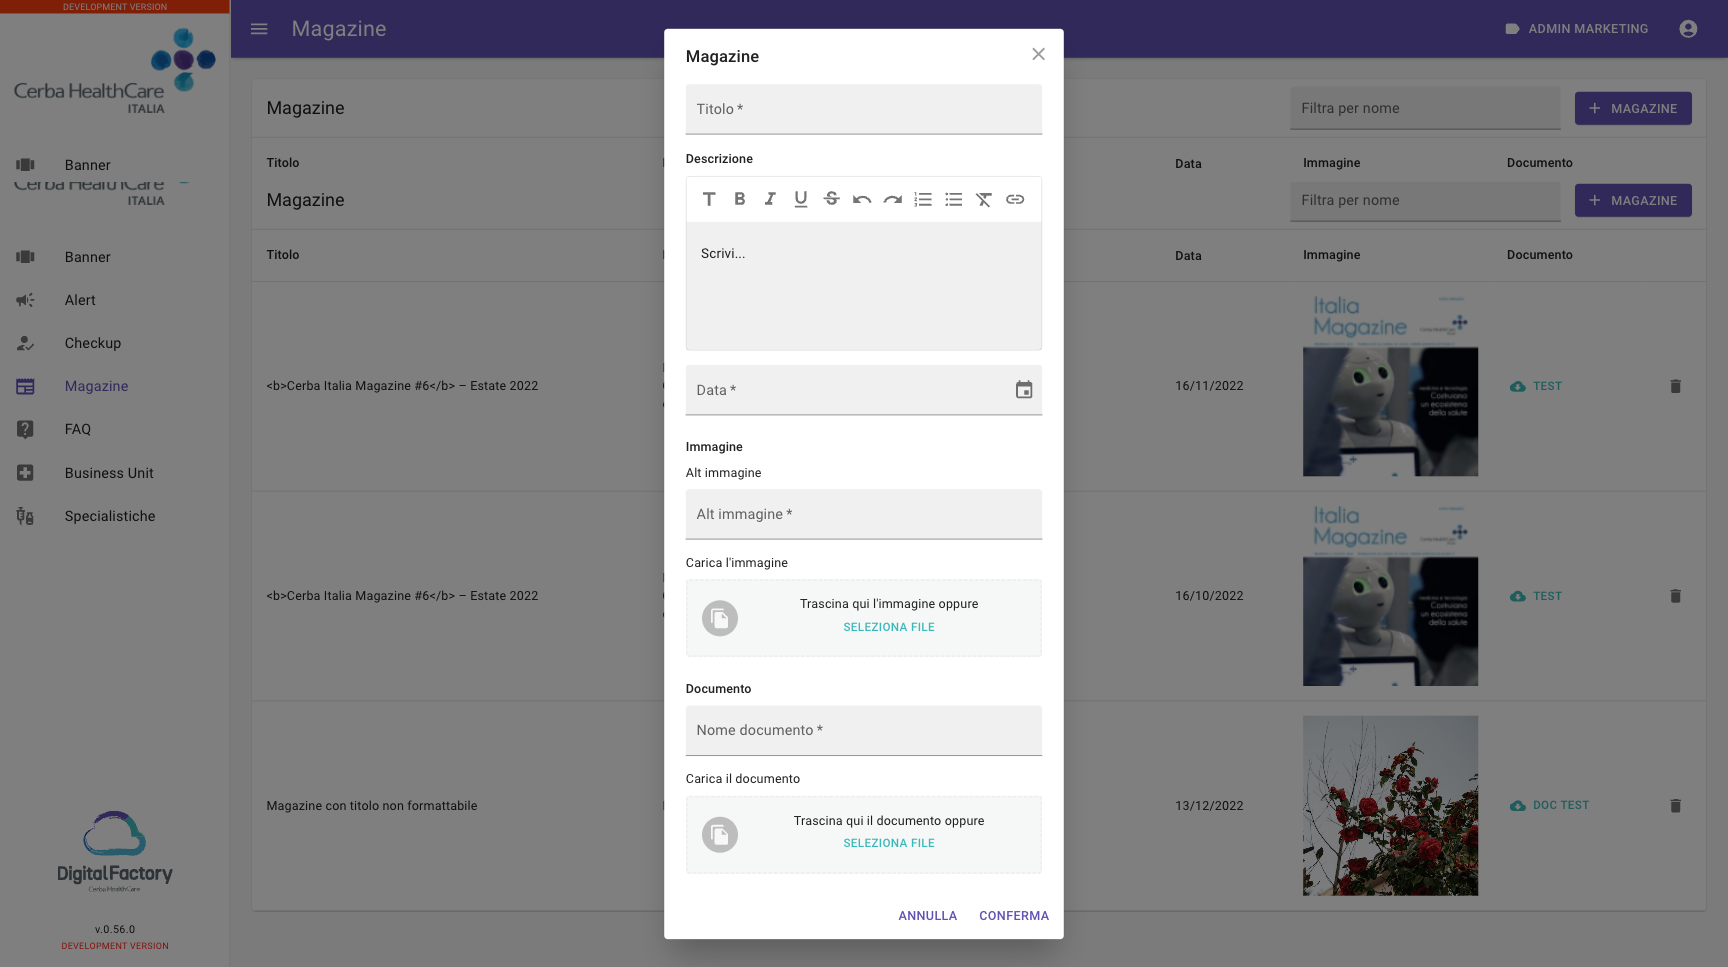
\includegraphics[width=0.7\textwidth]{images/capitolo5/f6_magazines/ModalMagazine_create.png} 
    \caption{Modale aggiunta nuovo magazine} 
    \label{fig:ModalMagazine_create}
\end{figure}

\begin{figure}[H]
    \centering
    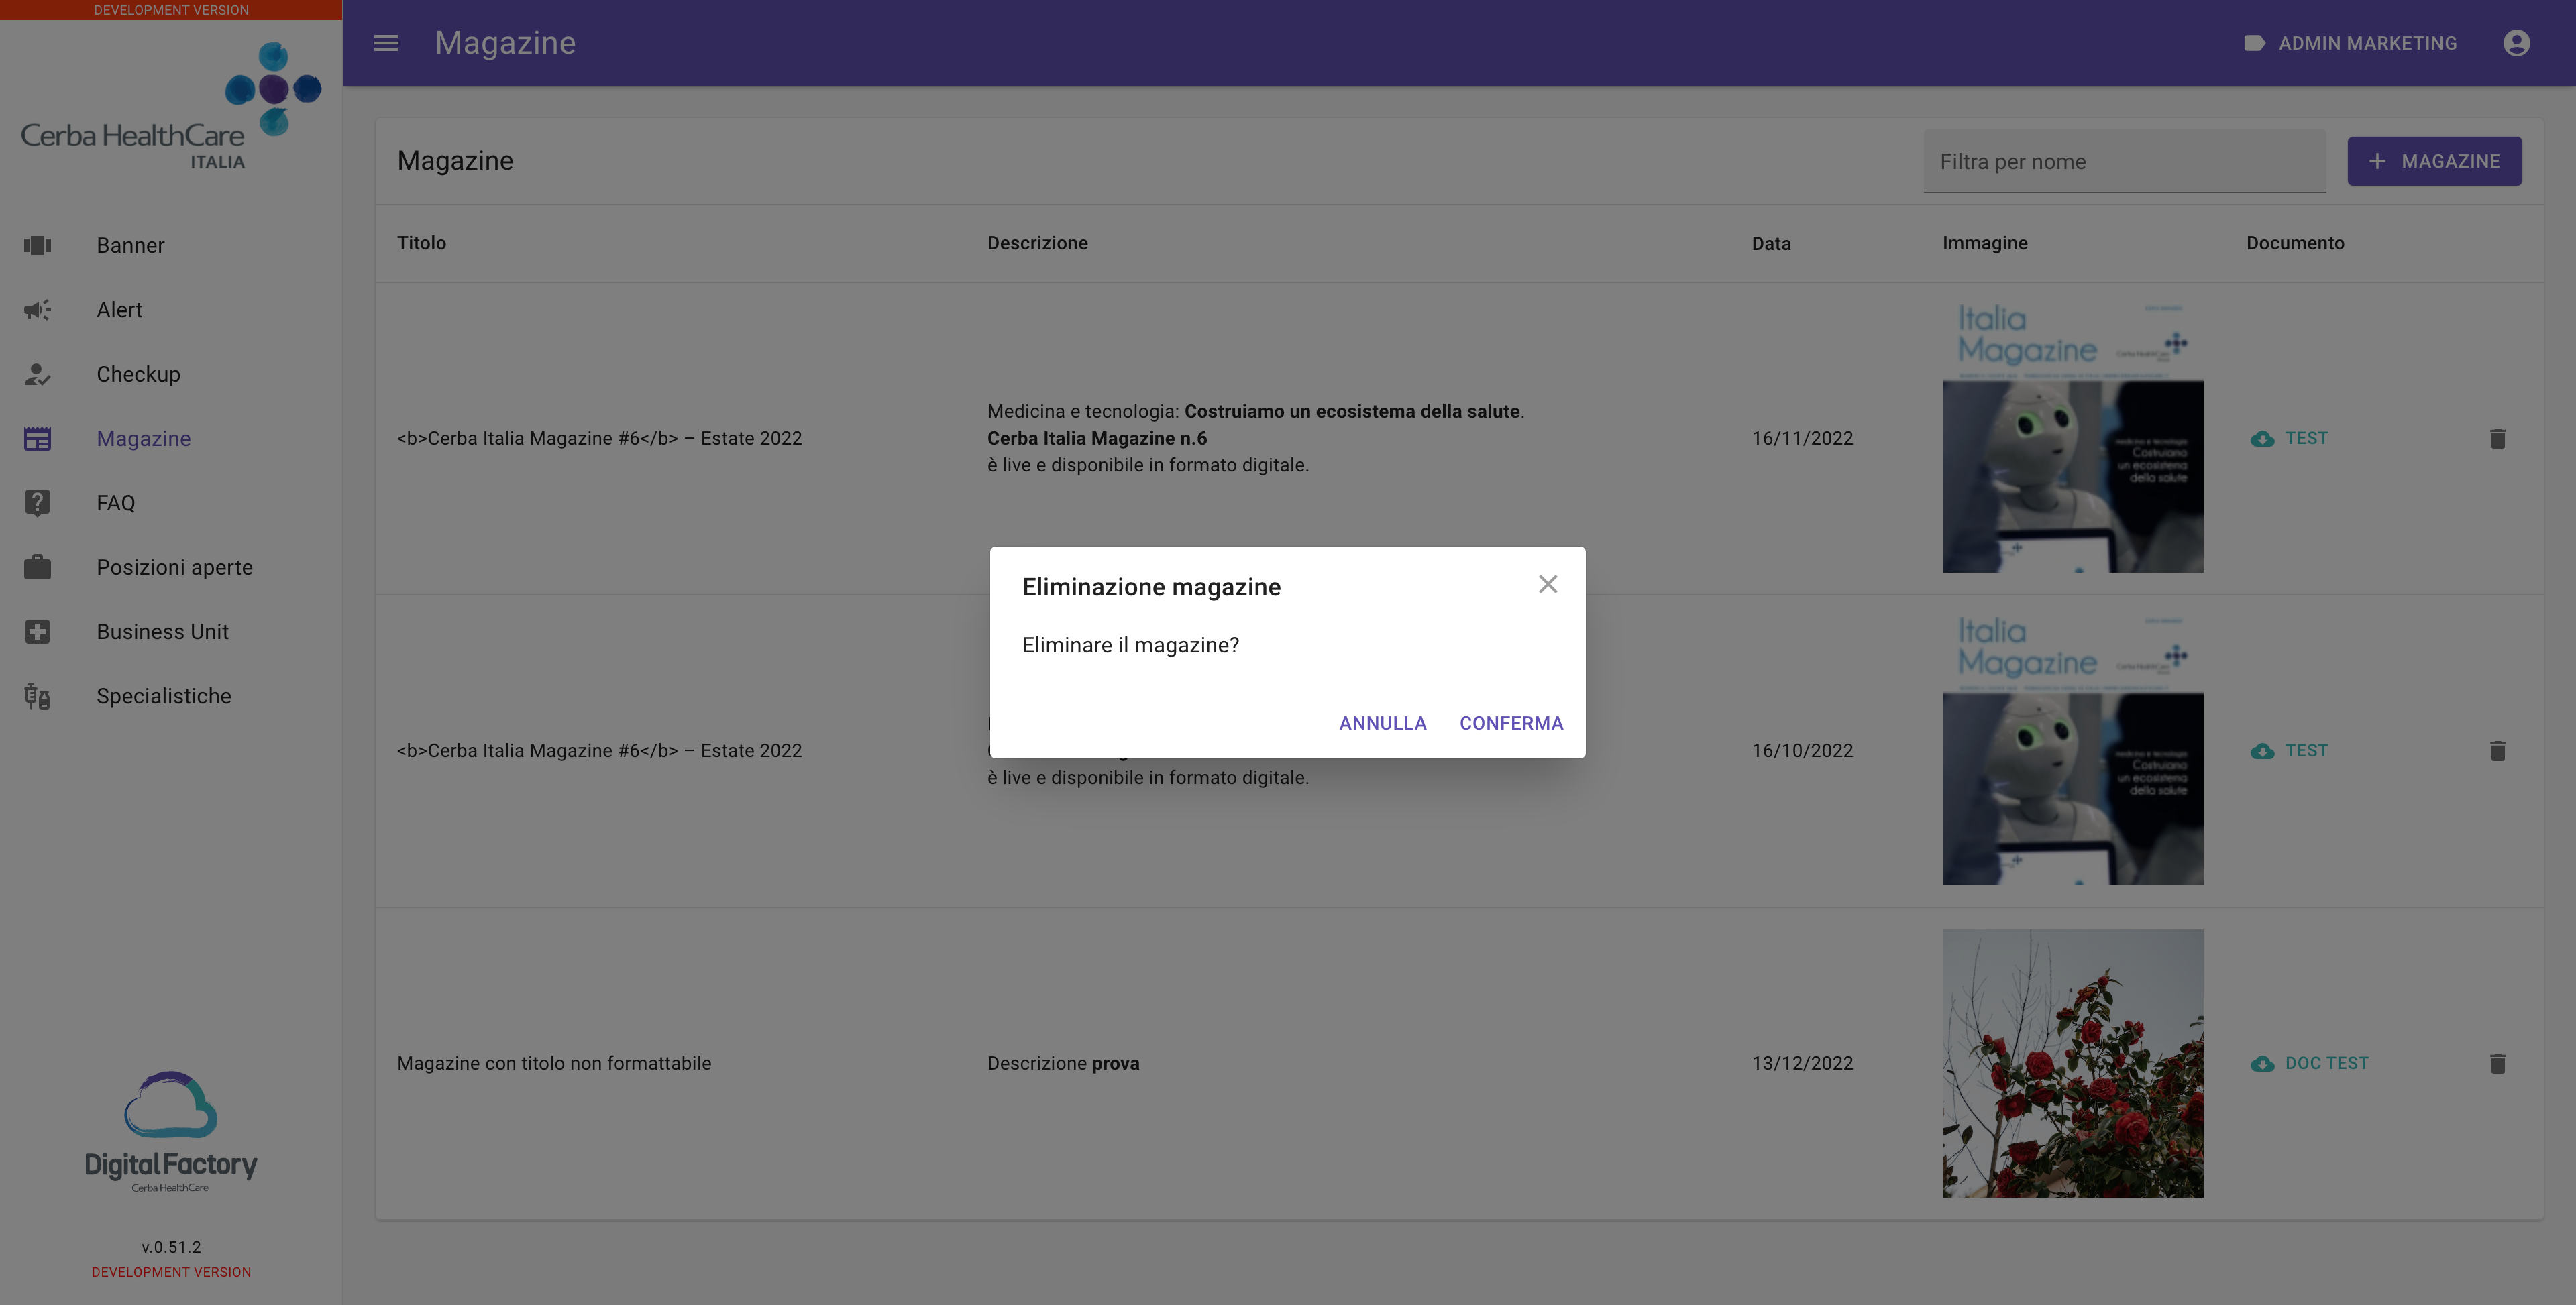
\includegraphics[width=0.75\textwidth]{images/capitolo5/f6_magazines/ModalMagazine_delete.png} 
    \caption{Modale eliminazione magazine esistente} 
    \label{fig:ModalMagazine_delete}
\end{figure}

\begin{figure}[H]
    \centering
    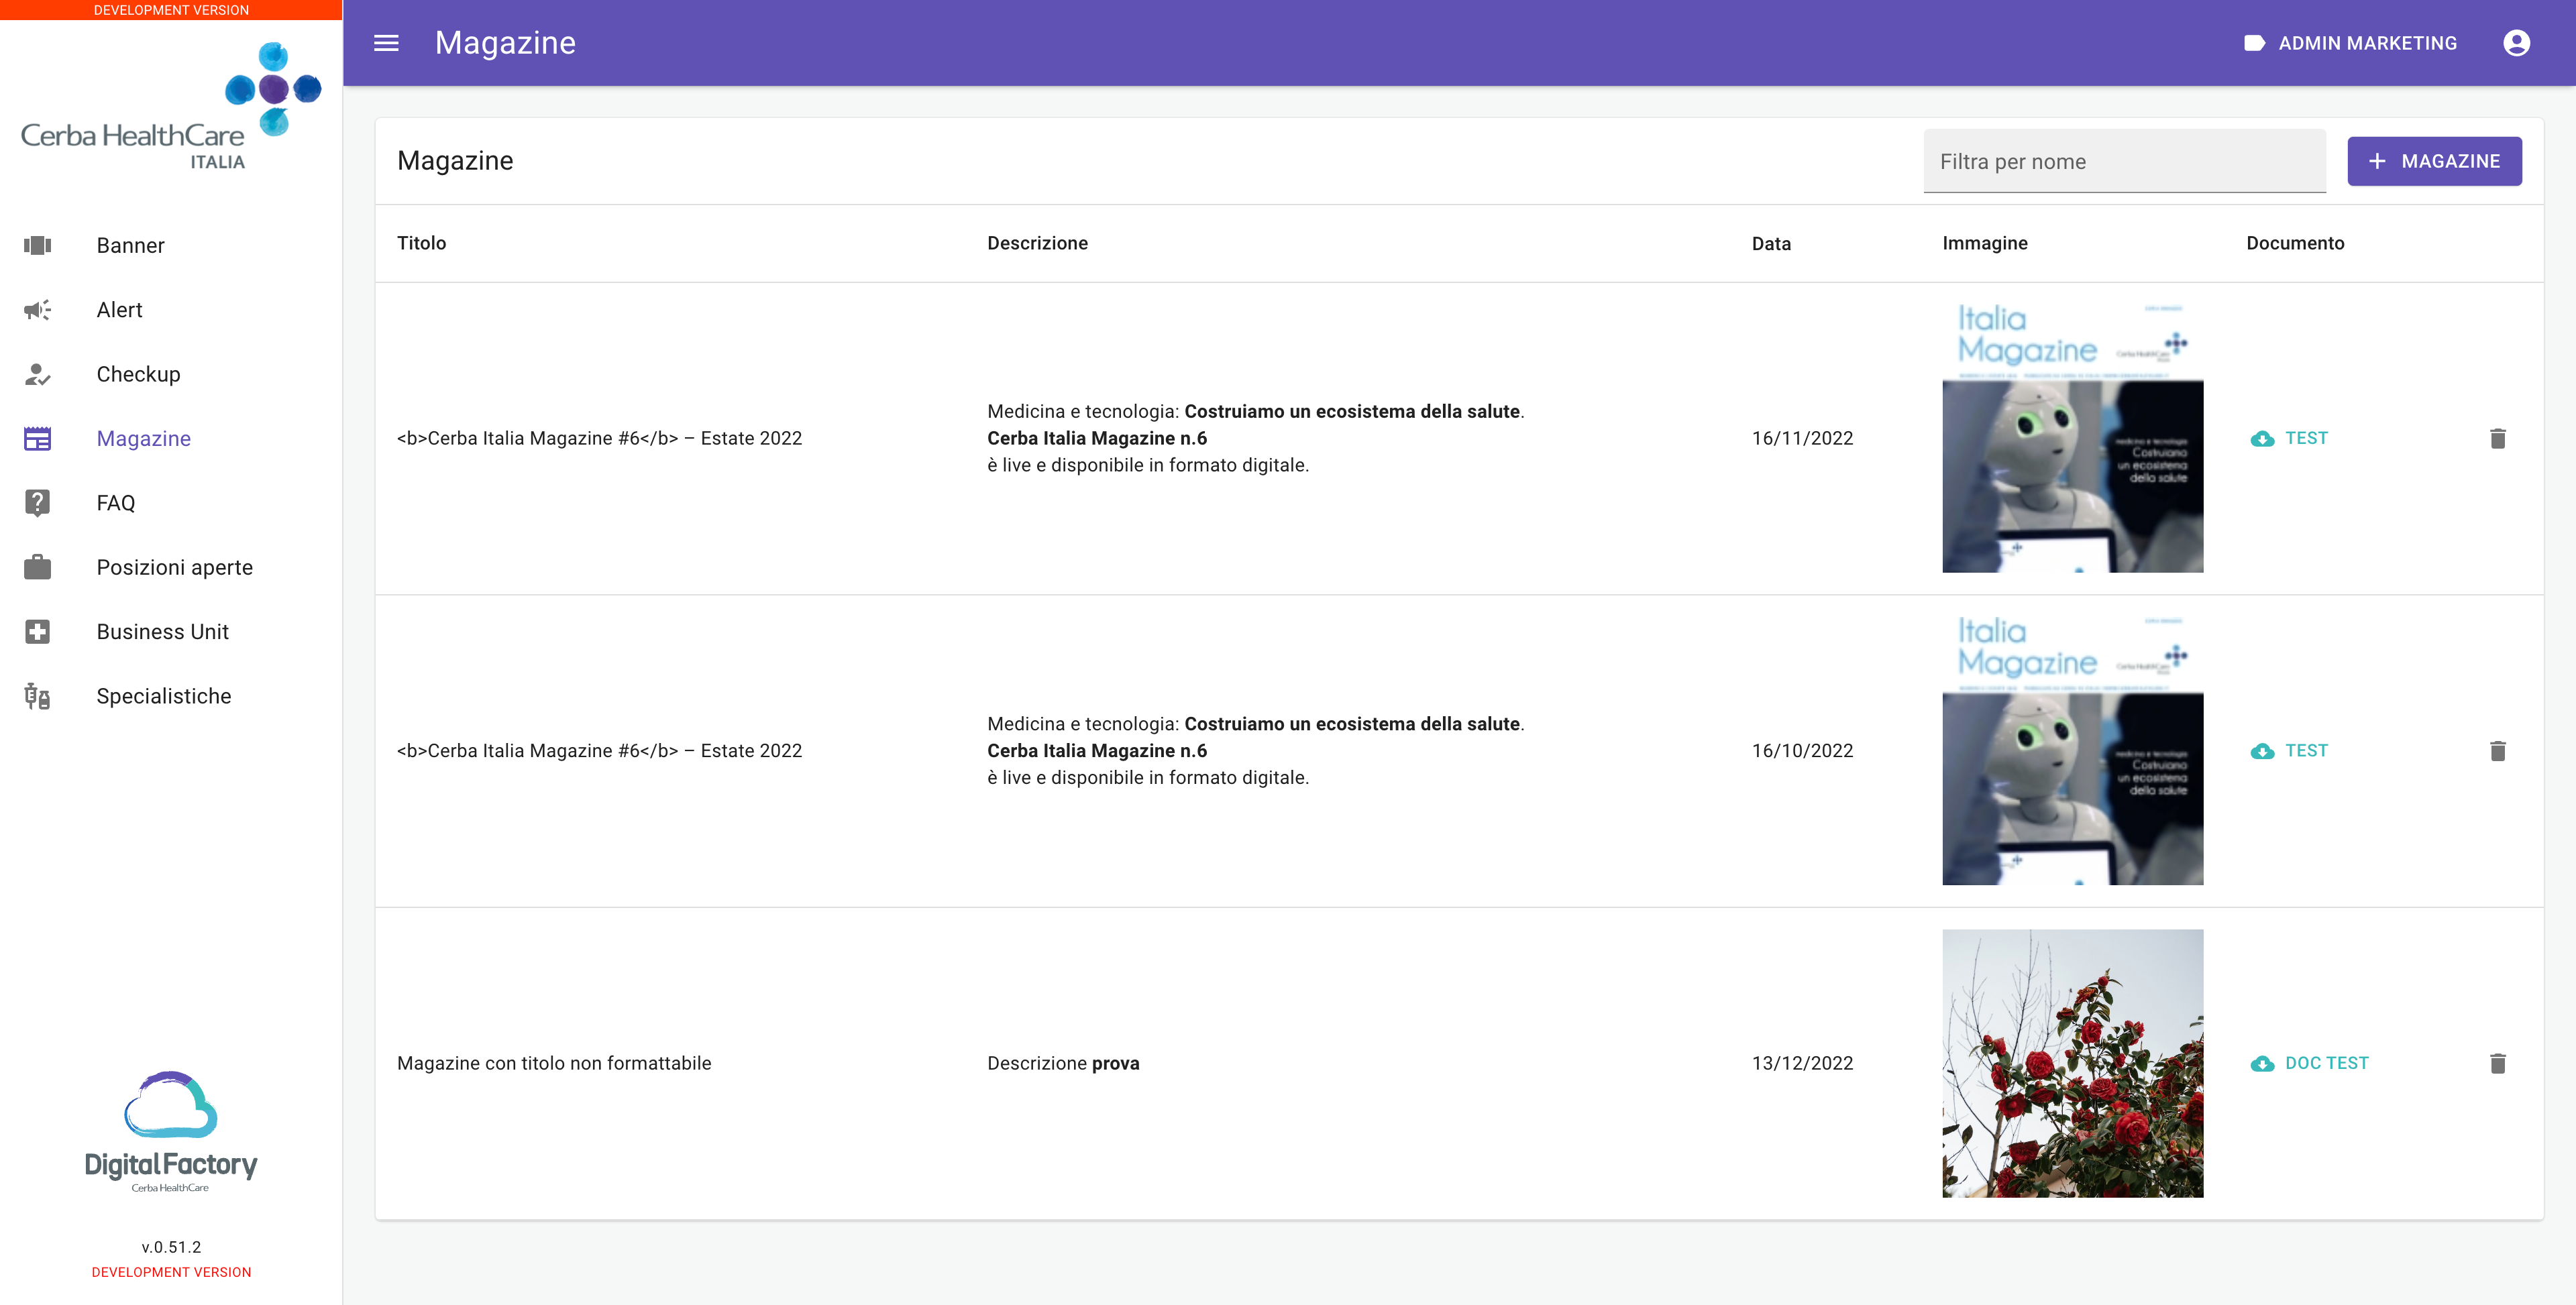
\includegraphics[width=0.75\textwidth]{images/capitolo5/f6_magazines/PageMagazines_searchEmpty.png} 
    \caption{Tabella magazine campo ricerca vuoto} 
    \label{fig:PageMagazine_searchEmpty}
\end{figure}

\begin{figure}[H]
    \centering
    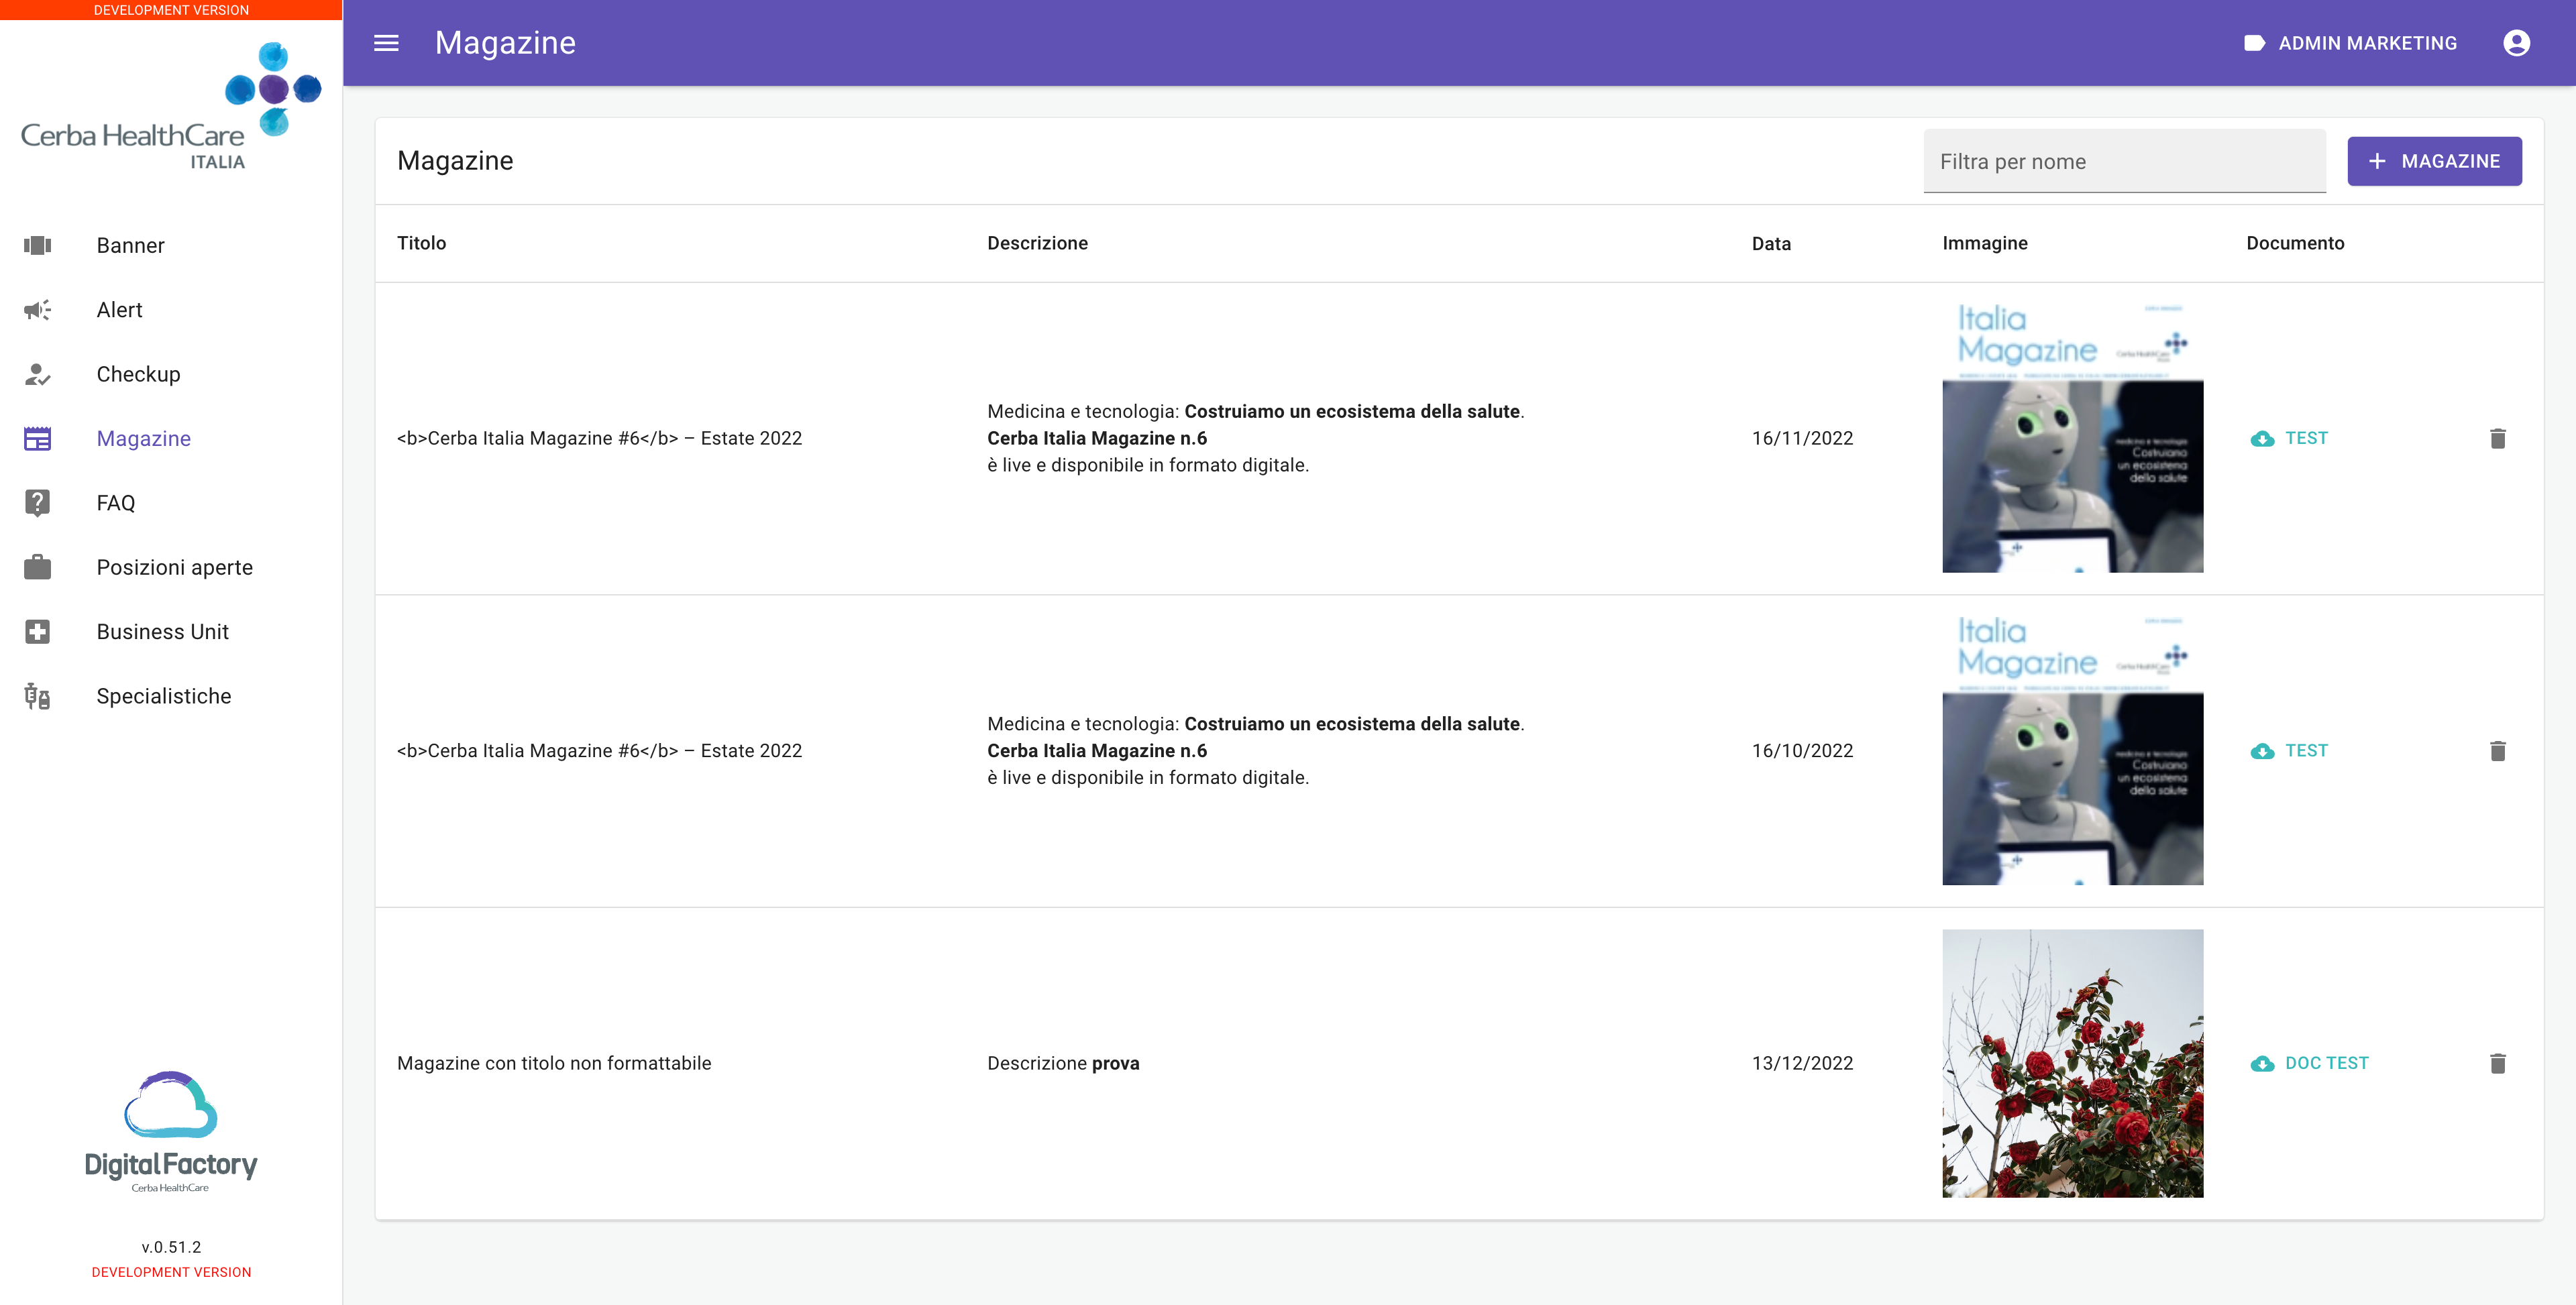
\includegraphics[width=0.75\textwidth]{images/capitolo5/f6_magazines/PageMagazines_searchEmpty.png} 
    \caption{Tabella magazine campo ricerca riempito} 
    \label{fig:PageMagazine_searchFilled}
\end{figure}

\subsection{F7: “FAQ”}
\subparagraph{Requisiti}
Aggiungere la sezione “FAQ” fra quelle previste per il ruolo utente \textit{marketing admin}.\\
Al suo interno, una tabella deve mostrare le FAQ esistenti in una lista semplice e riportarne le proprietà “Domanda”, “Risposta” e “Categoria”.\\
Deve essere possibile aggiungere, modificare o eliminare una FAQ.\\
Solamente per la proprietà “Risposta” deve essere fornita la possibilità di formattare il testo.\\
L'\textit{header} della tabella delle FAQ deve essere dotato di un campo di ricerca. Questo deve essere in grado di filtrare per domanda e posizionato alla sinistra del bottone per l'aggiunta di una nuova FAQ.

% \paragraph{\textit{Output} grafico}
% \begin{figure}[H]
%     \centering
%     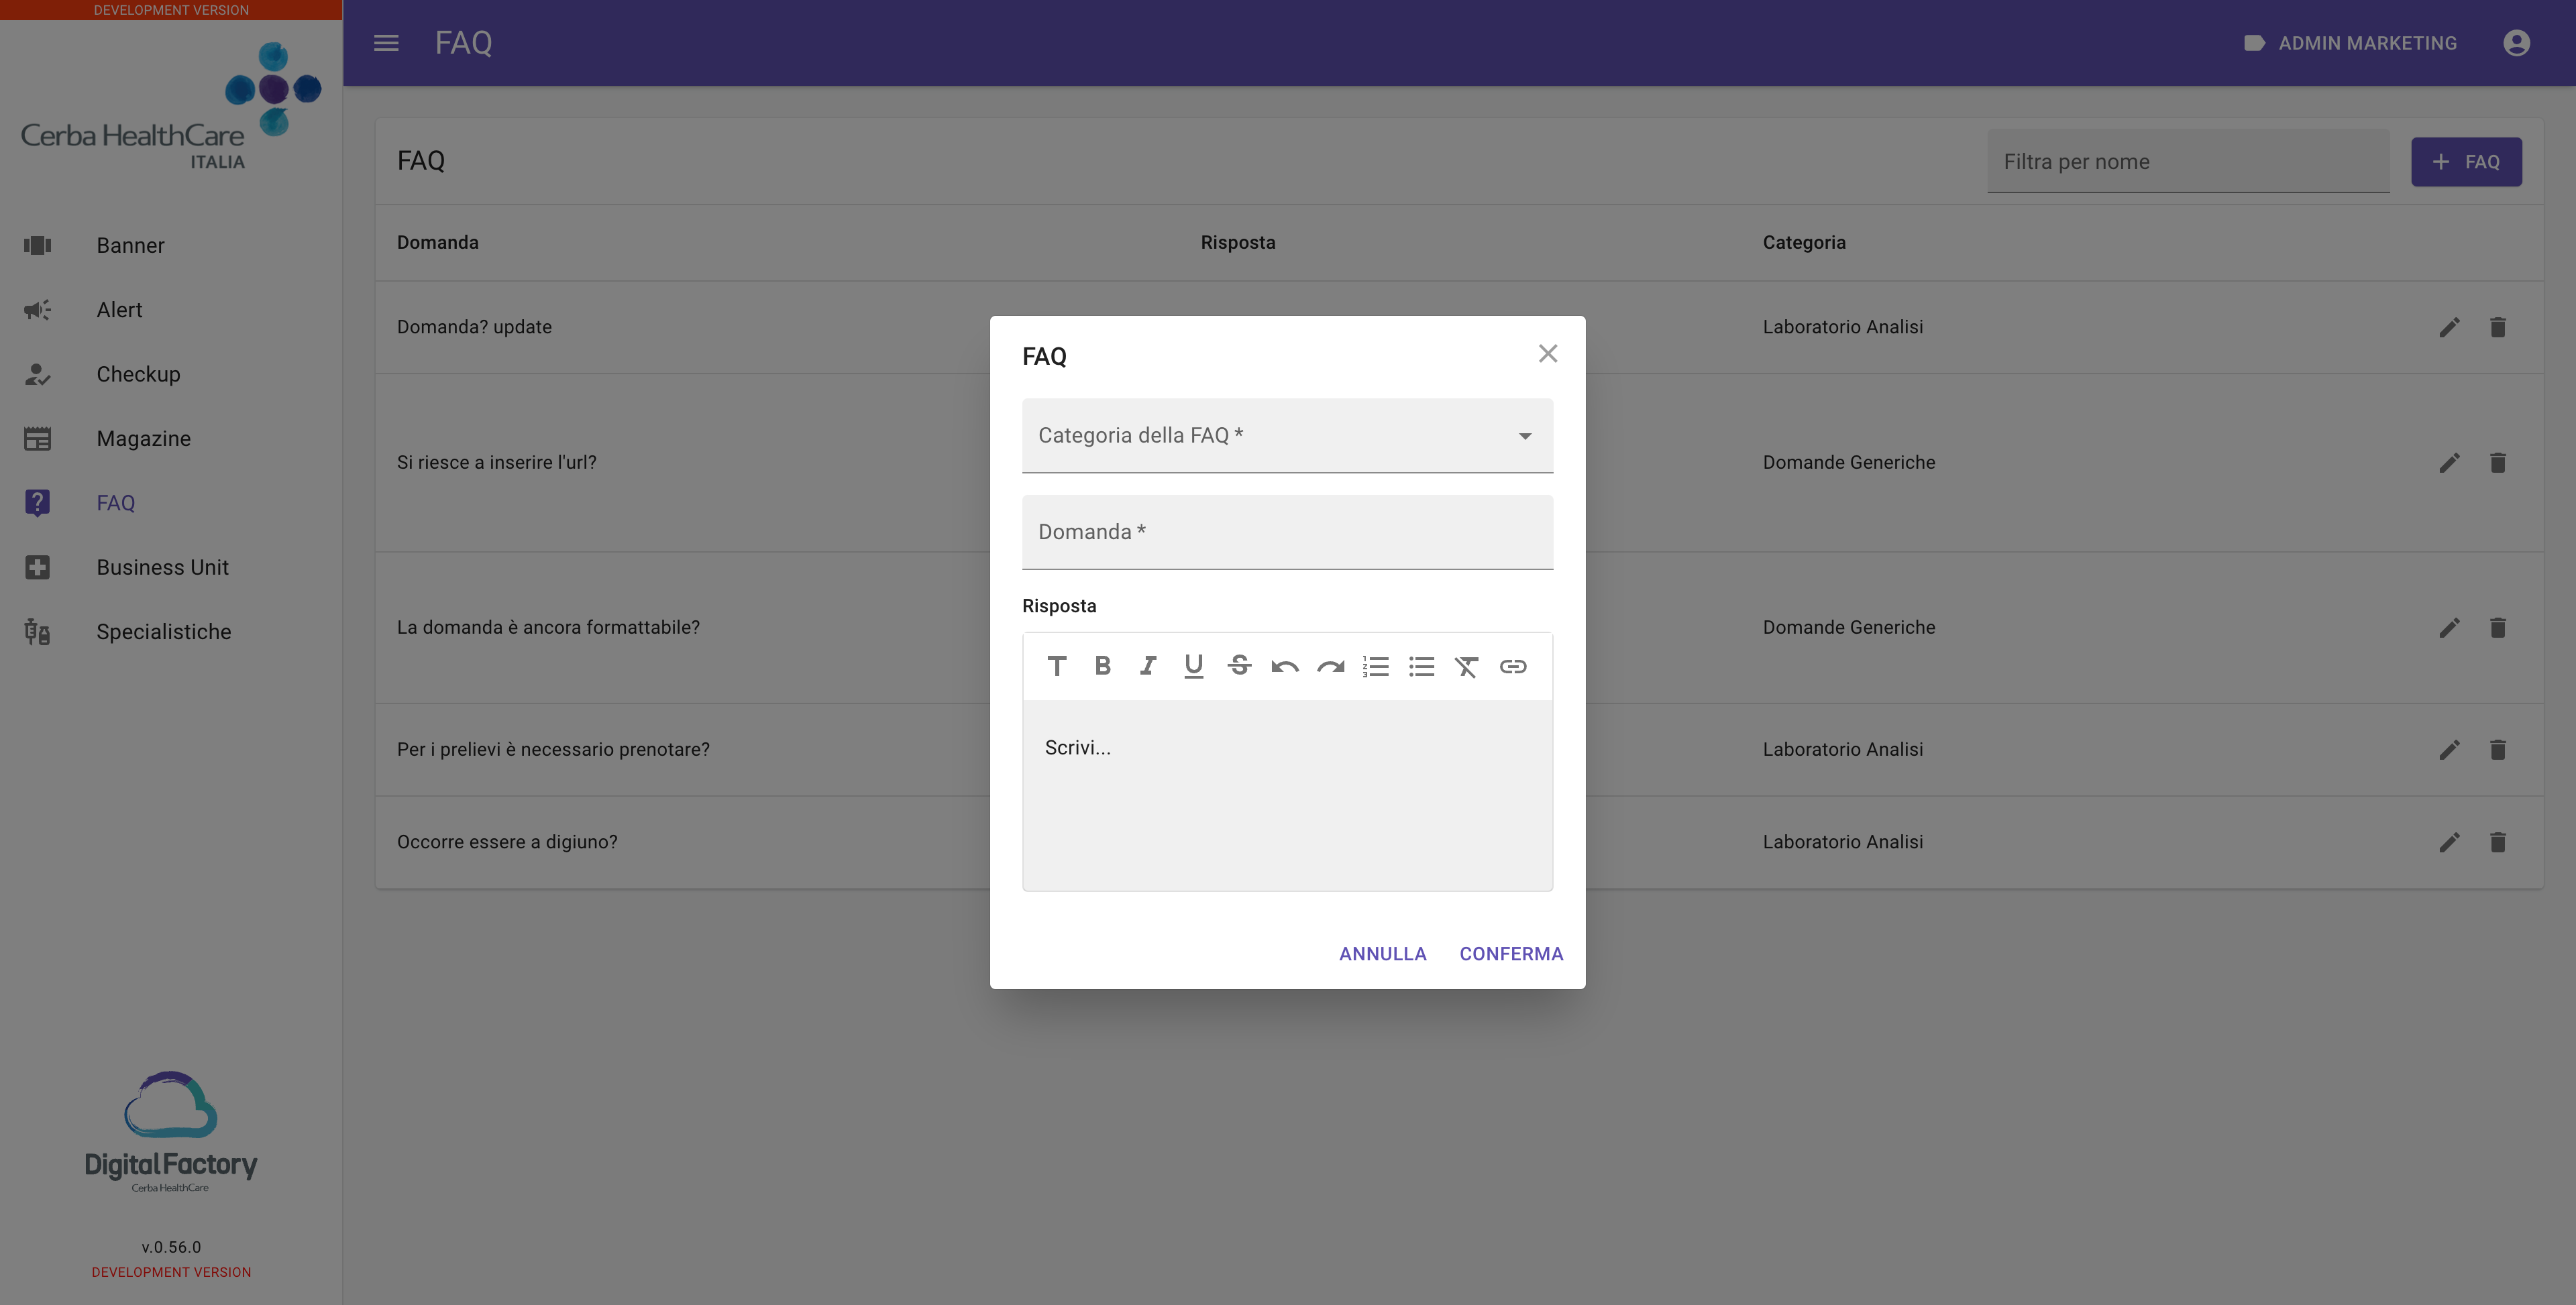
\includegraphics[width=0.75\textwidth]{images/capitolo5/f7_faqs/ModalFaq_create.png} 
%     \caption{Modale aggiunta nuova faq} 
%     \label{fig:ModalFaq_create}
% \end{figure}

% \begin{figure}[H]
%     \centering
%     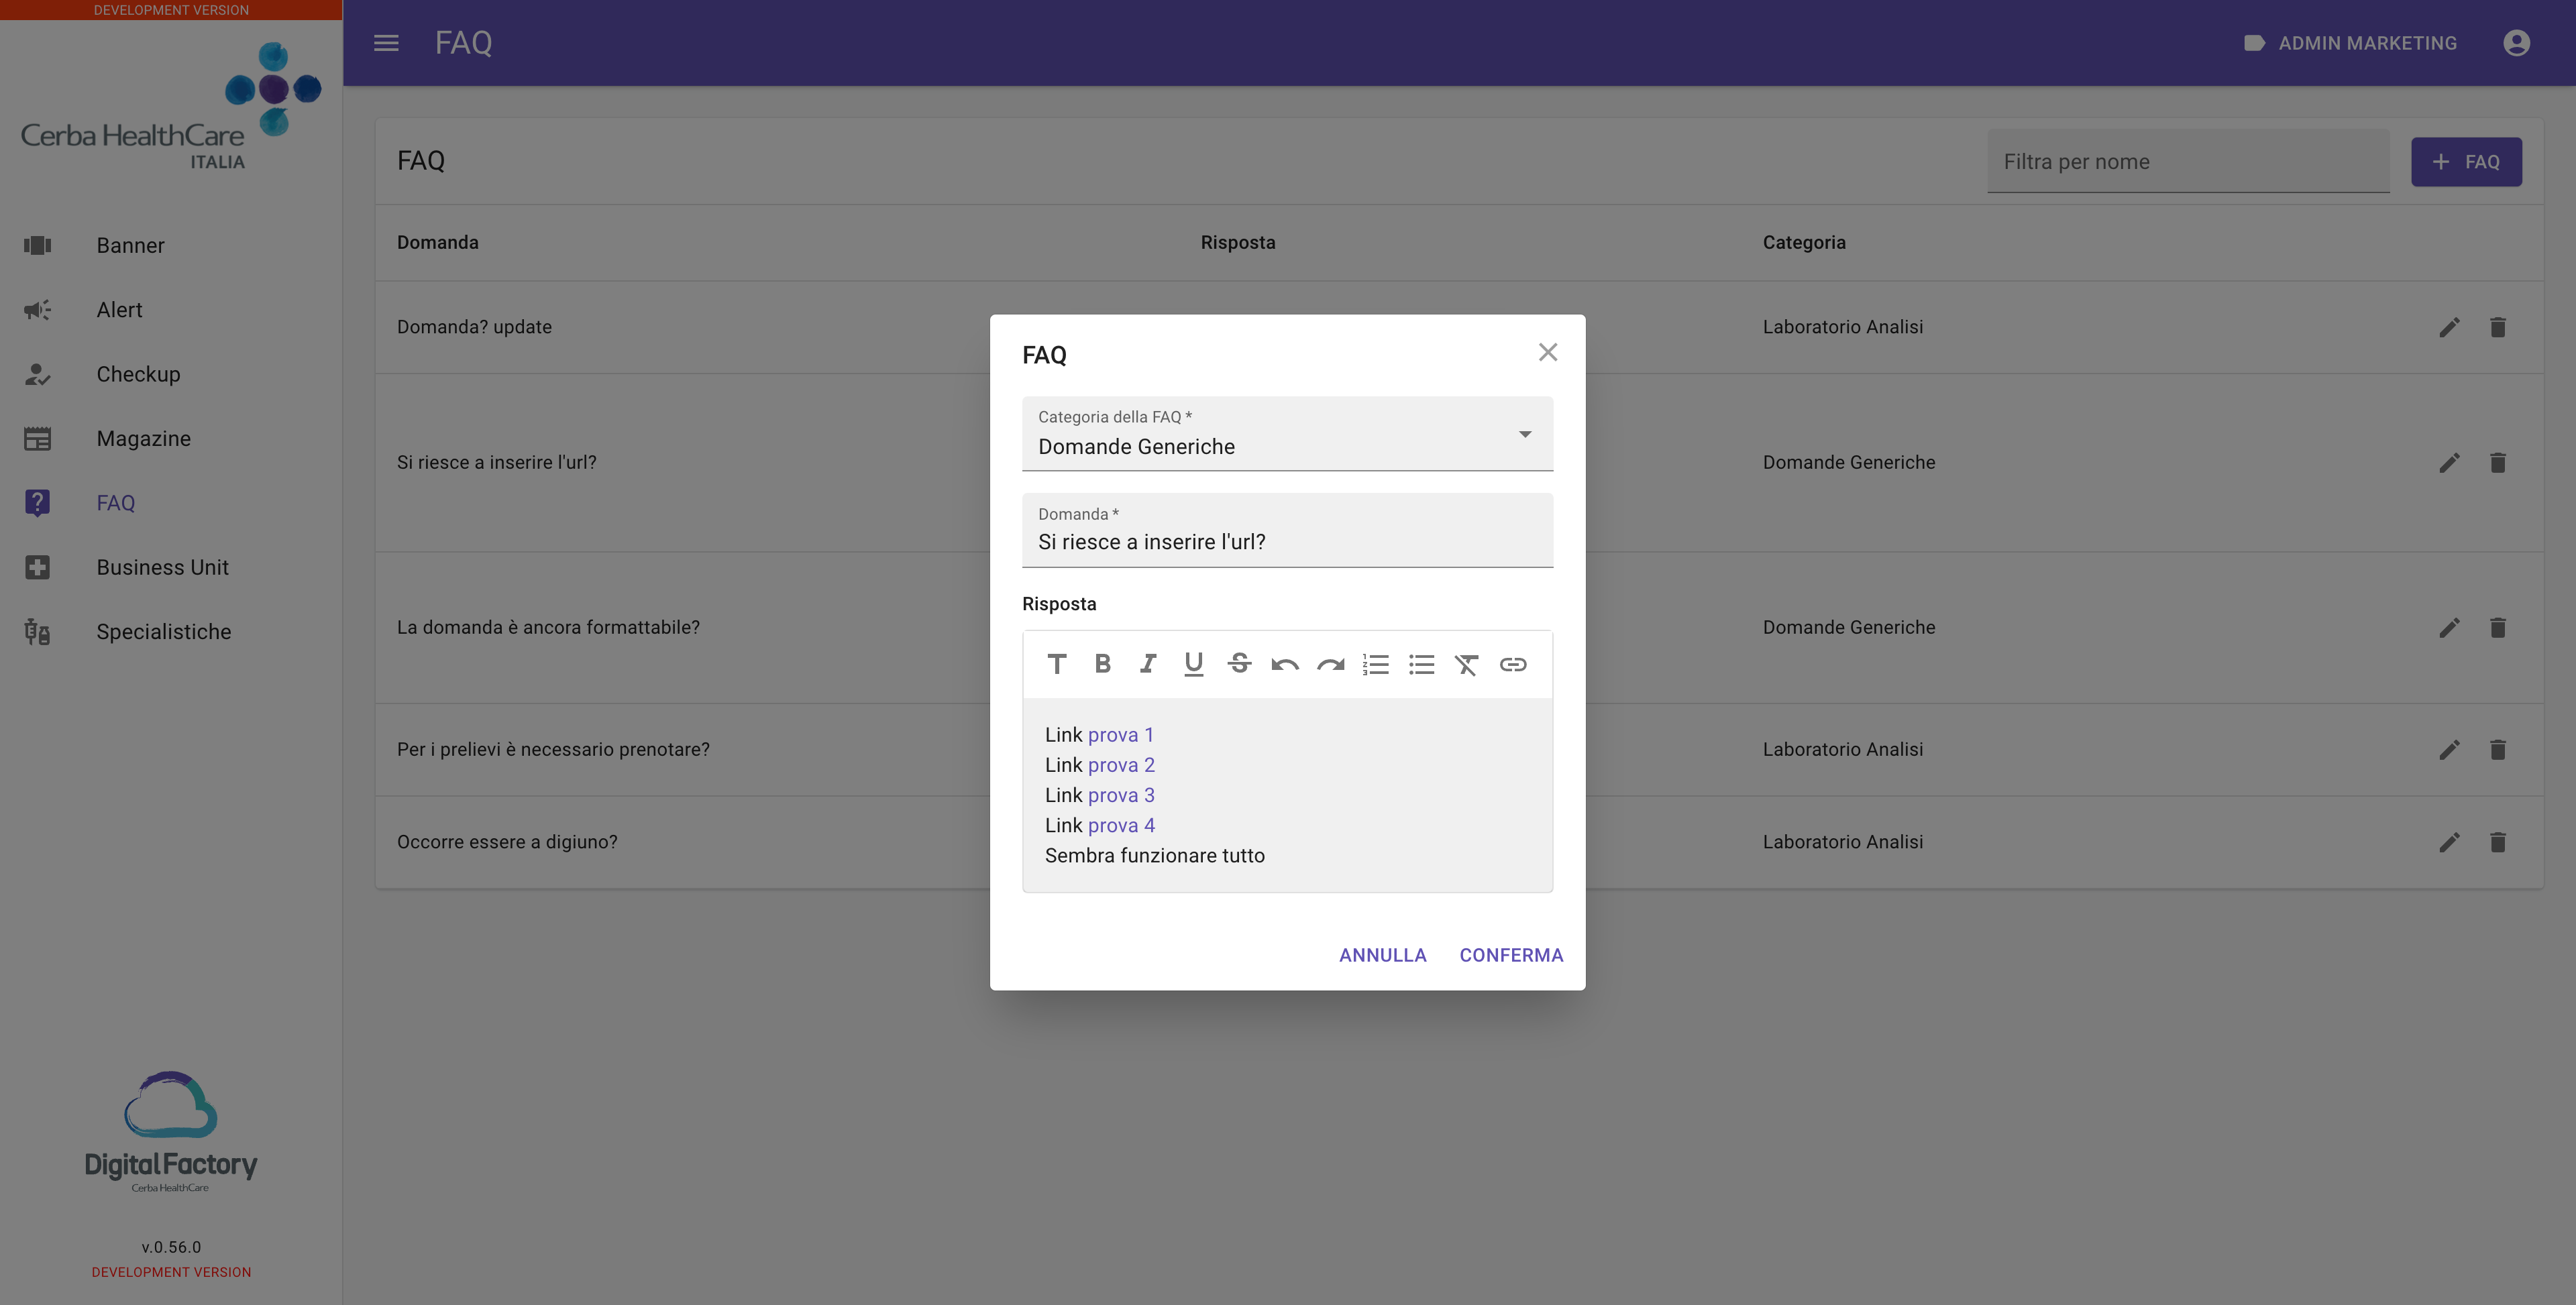
\includegraphics[width=0.75\textwidth]{images/capitolo5/f7_faqs/ModalFaq_edit.png} 
%     \caption{Modale modifica faq esistente} 
%     \label{fig:ModalFaq_edit}
% \end{figure}

% \begin{figure}[H]
%     \centering
%     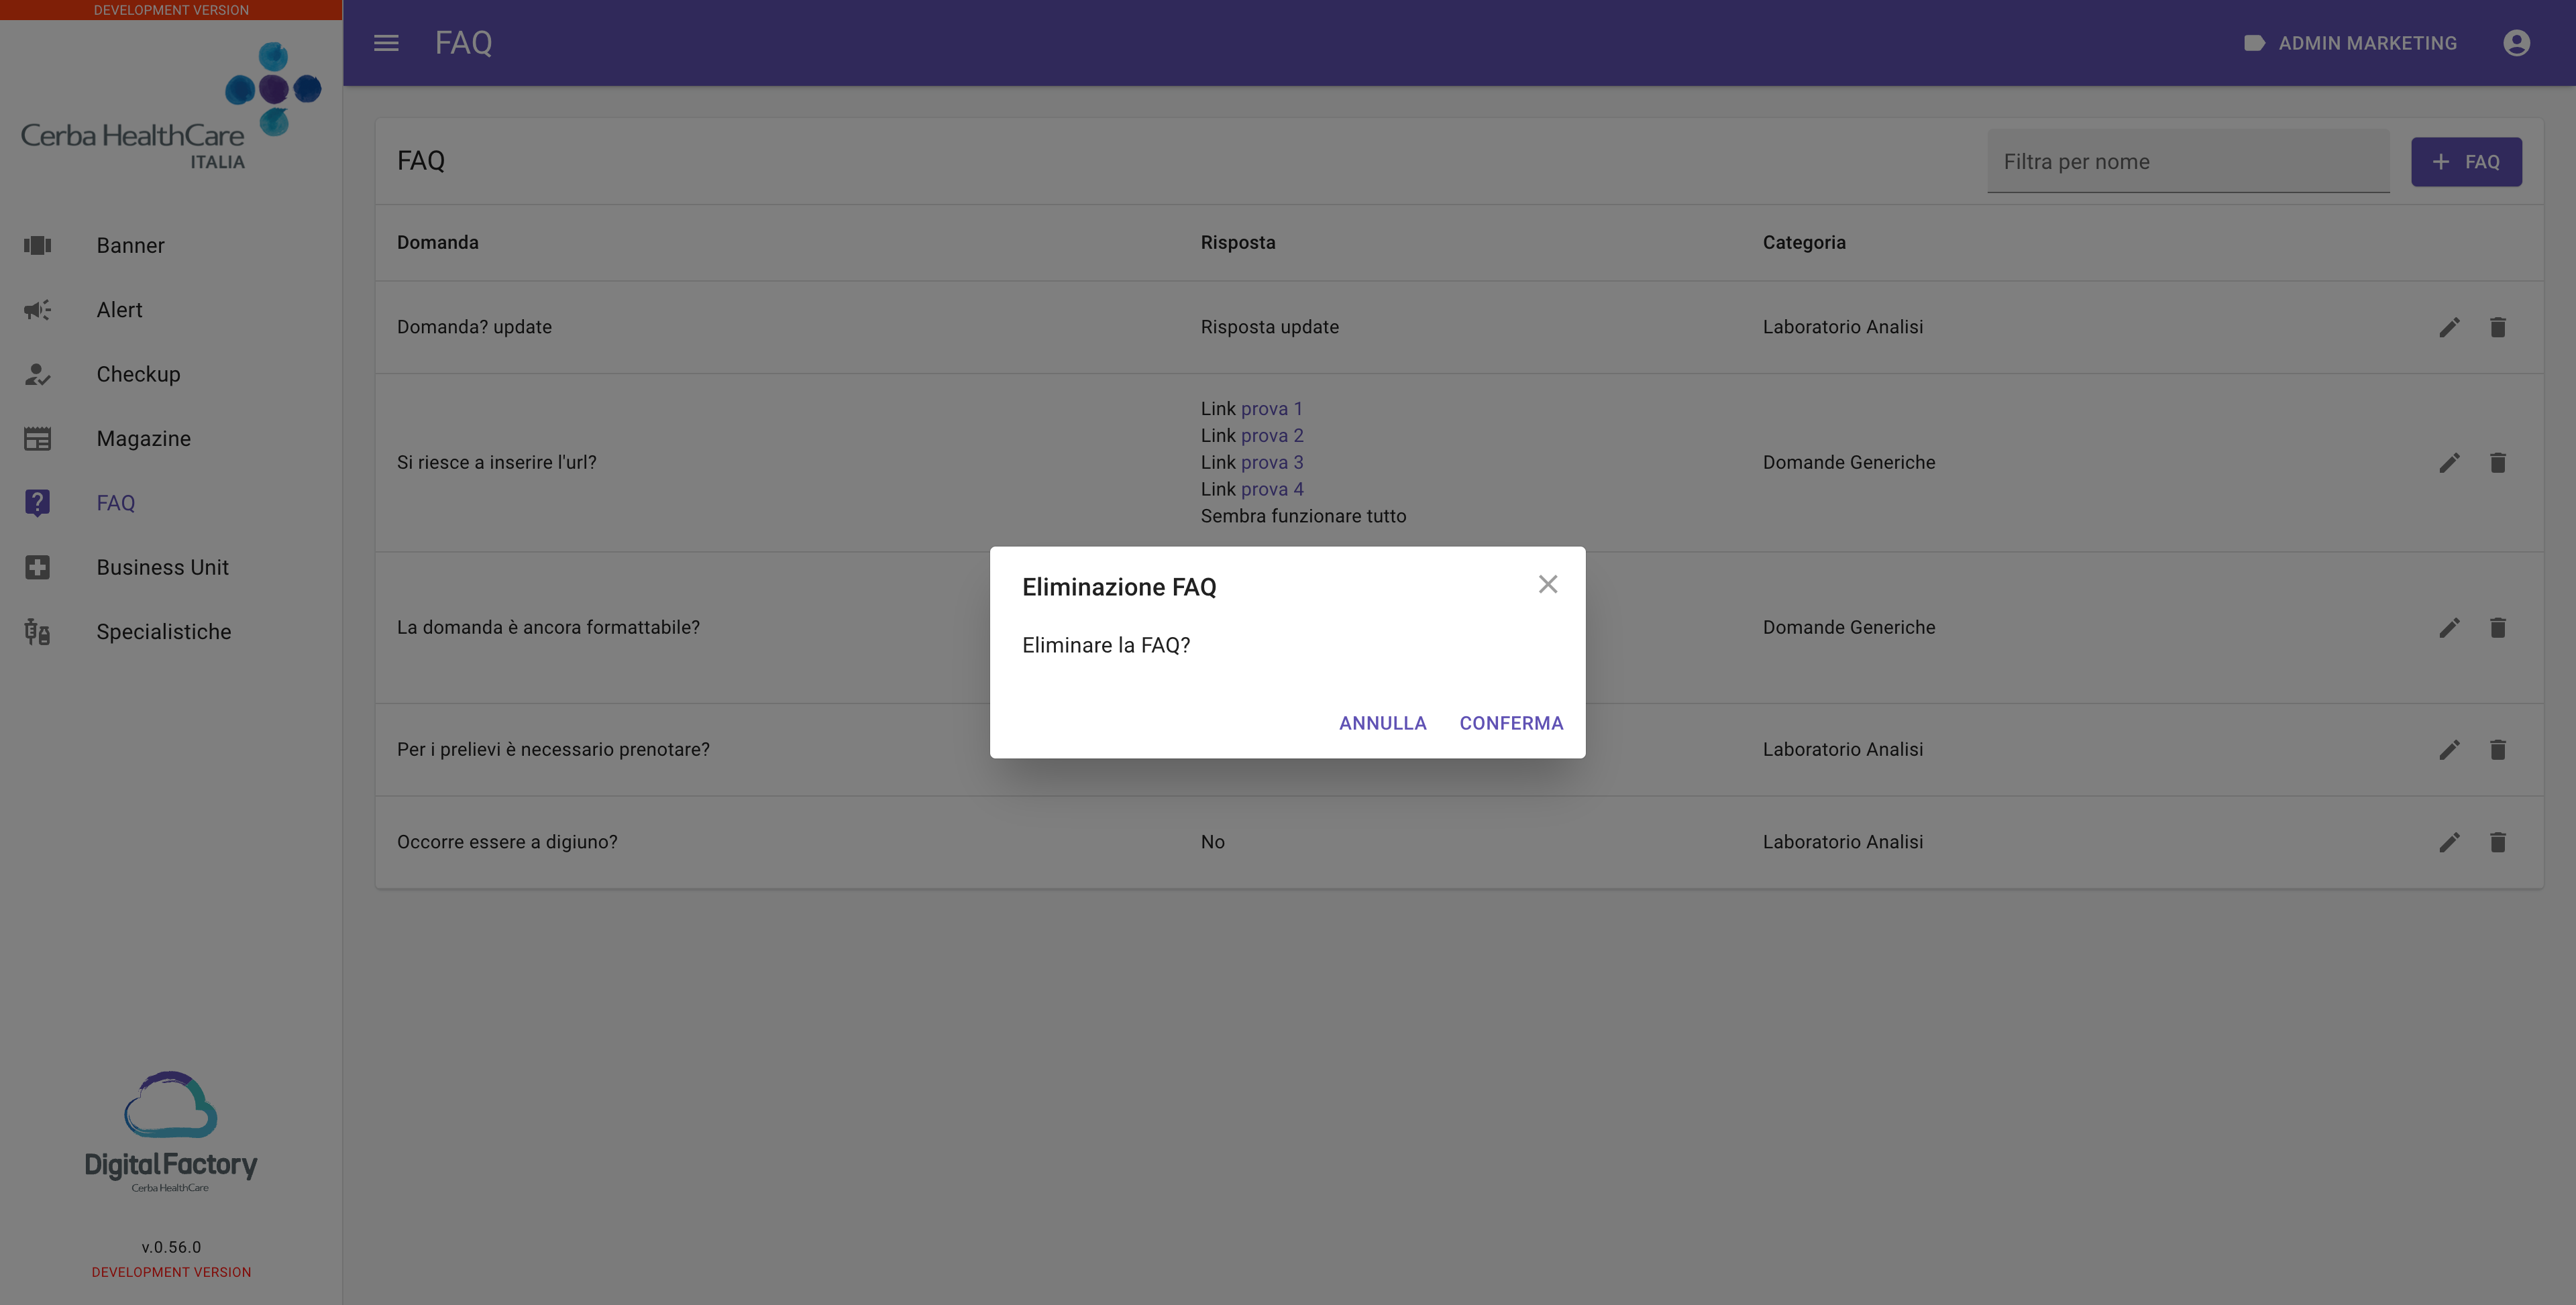
\includegraphics[width=0.75\textwidth]{images/capitolo5/f7_faqs/ModalFaq_delete.png} 
%     \caption{Modale eliminazione faq esistente} 
%     \label{fig:ModalFaq_edit}
% \end{figure}

% \begin{figure}[H]
%     \centering
%     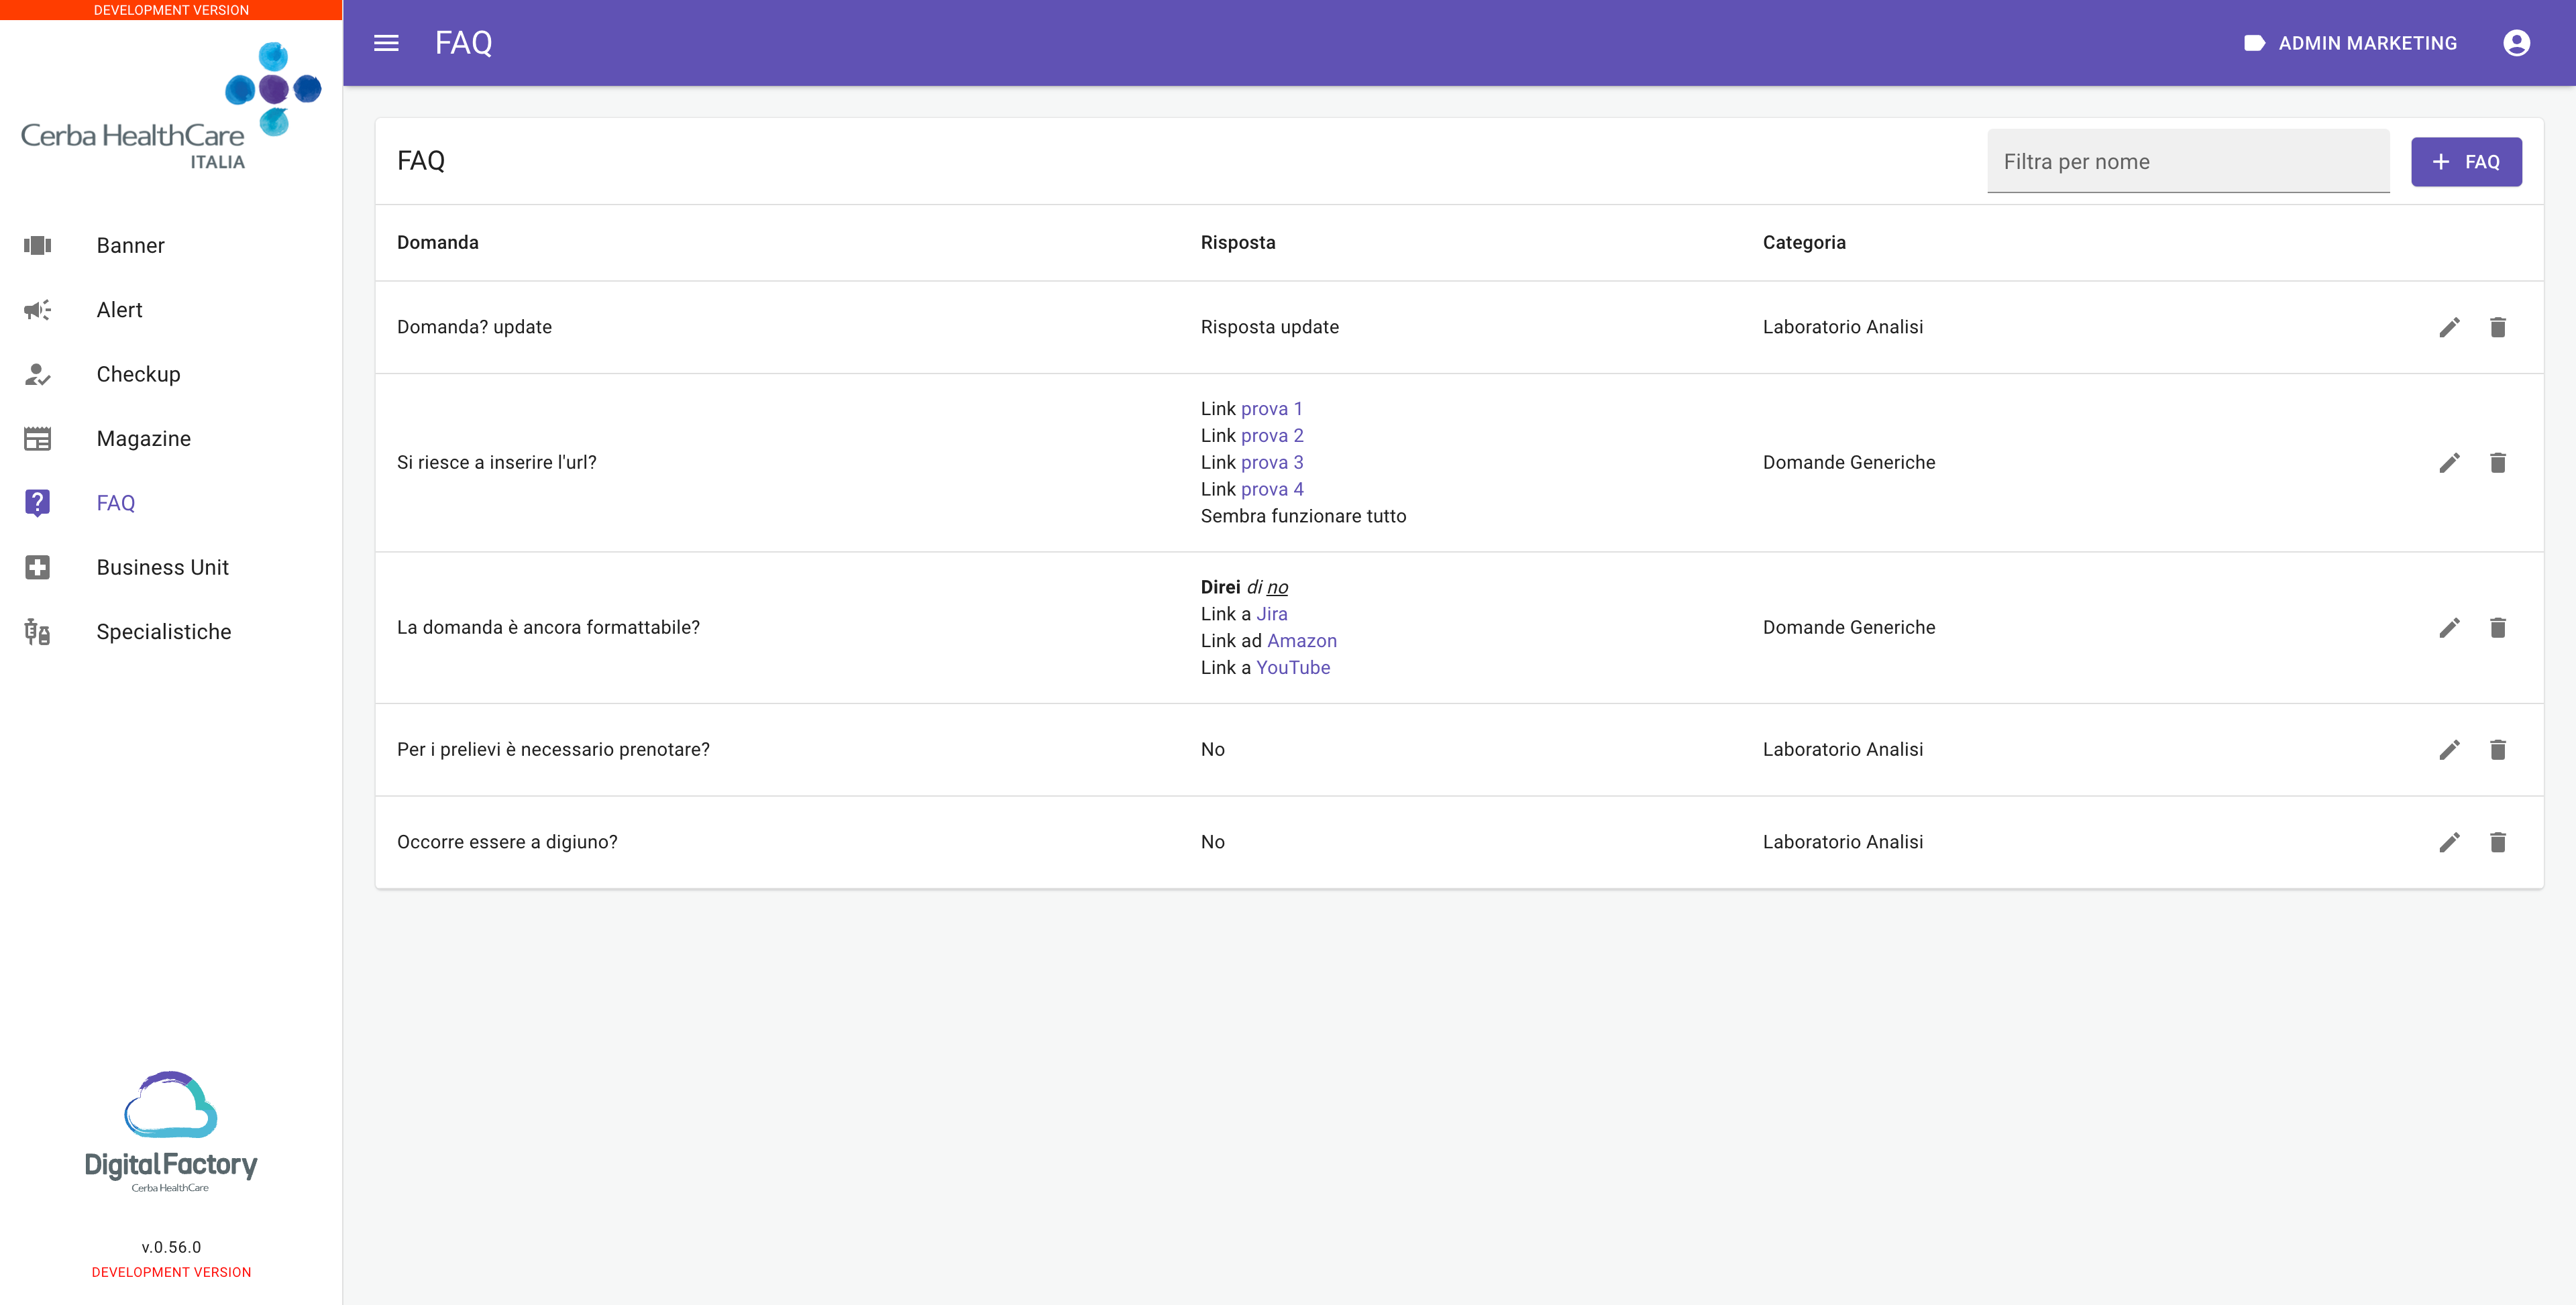
\includegraphics[width=0.75\textwidth]{images/capitolo5/f7_faqs/PageFaq_searchEmpty.png} 
%     \caption{Tabella faq campo ricerca vuoto} 
%     \label{fig:PageFaq_searchEmpty}
% \end{figure}

% \begin{figure}[H]
%     \centering
%     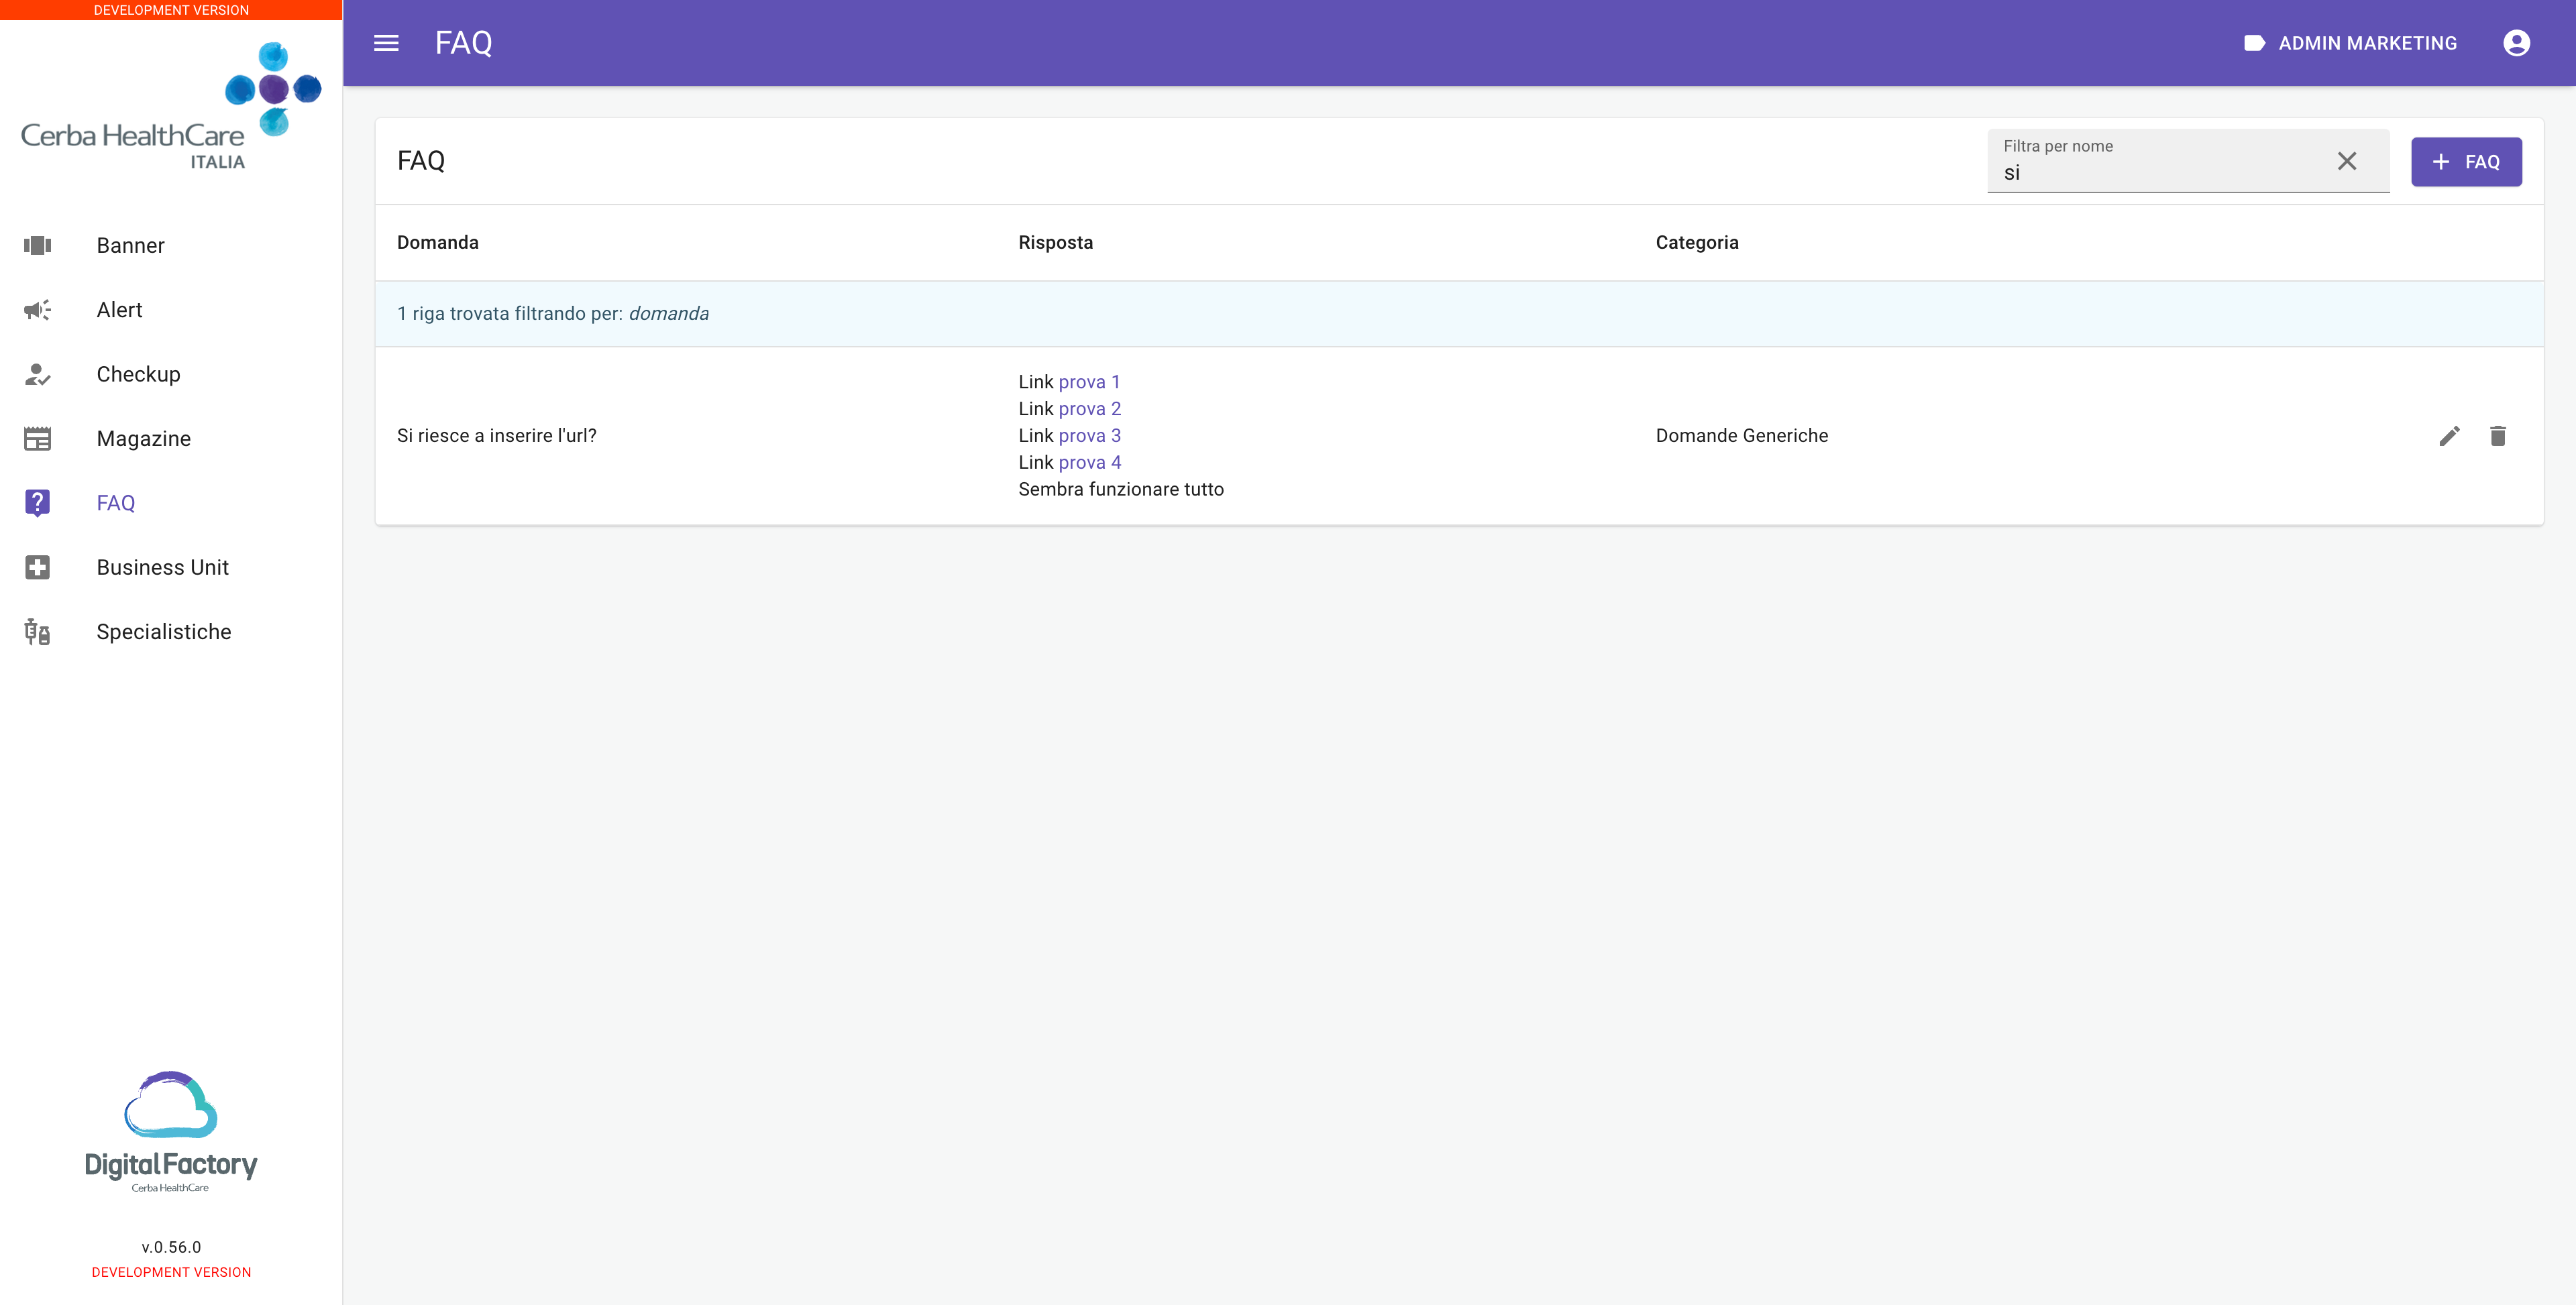
\includegraphics[width=0.75\textwidth]{images/capitolo5/f7_faqs/PageFaq_searchFilled.png} 
%     \caption{Tabella faq campo ricerca riempito} 
%     \label{fig:PageFaq_searchFilled}
% \end{figure}

\subsection{F8: “Business Unit”}
\subparagraph{Requisiti}
Aggiungere la sezione “Business Unit” fra quelle previste per il ruolo utente \textit{marketing admin}.\\
Al suo interno, una tabella deve mostrare le \textit{business unit} (BU) esistenti in una lista semplice e riportarne la proprietà “Nome”.\\
L'\textit{header} della tabella delle BU deve essere dotato di un campo di ricerca. Questo deve essere in grado di filtrare per nome e posizionato all'estrema destra dell'\textit{header} della tabella.\\
Ogni BU deve essere dotata di una pagina di dettaglio alla quale si accede cliccando sul link posto in concomitanza del nome. Qui, deve essere possibile modificare e visualizzare la descrizione, campo che deve poter essere formattato; sempre all'interno della pagina di dettaglio, si devono poter aggiungere, visualizzare ed eliminare un'immagine e un'icona.

\paragraph{\textit{Output} grafico}
\begin{figure}[H]
    \centering
    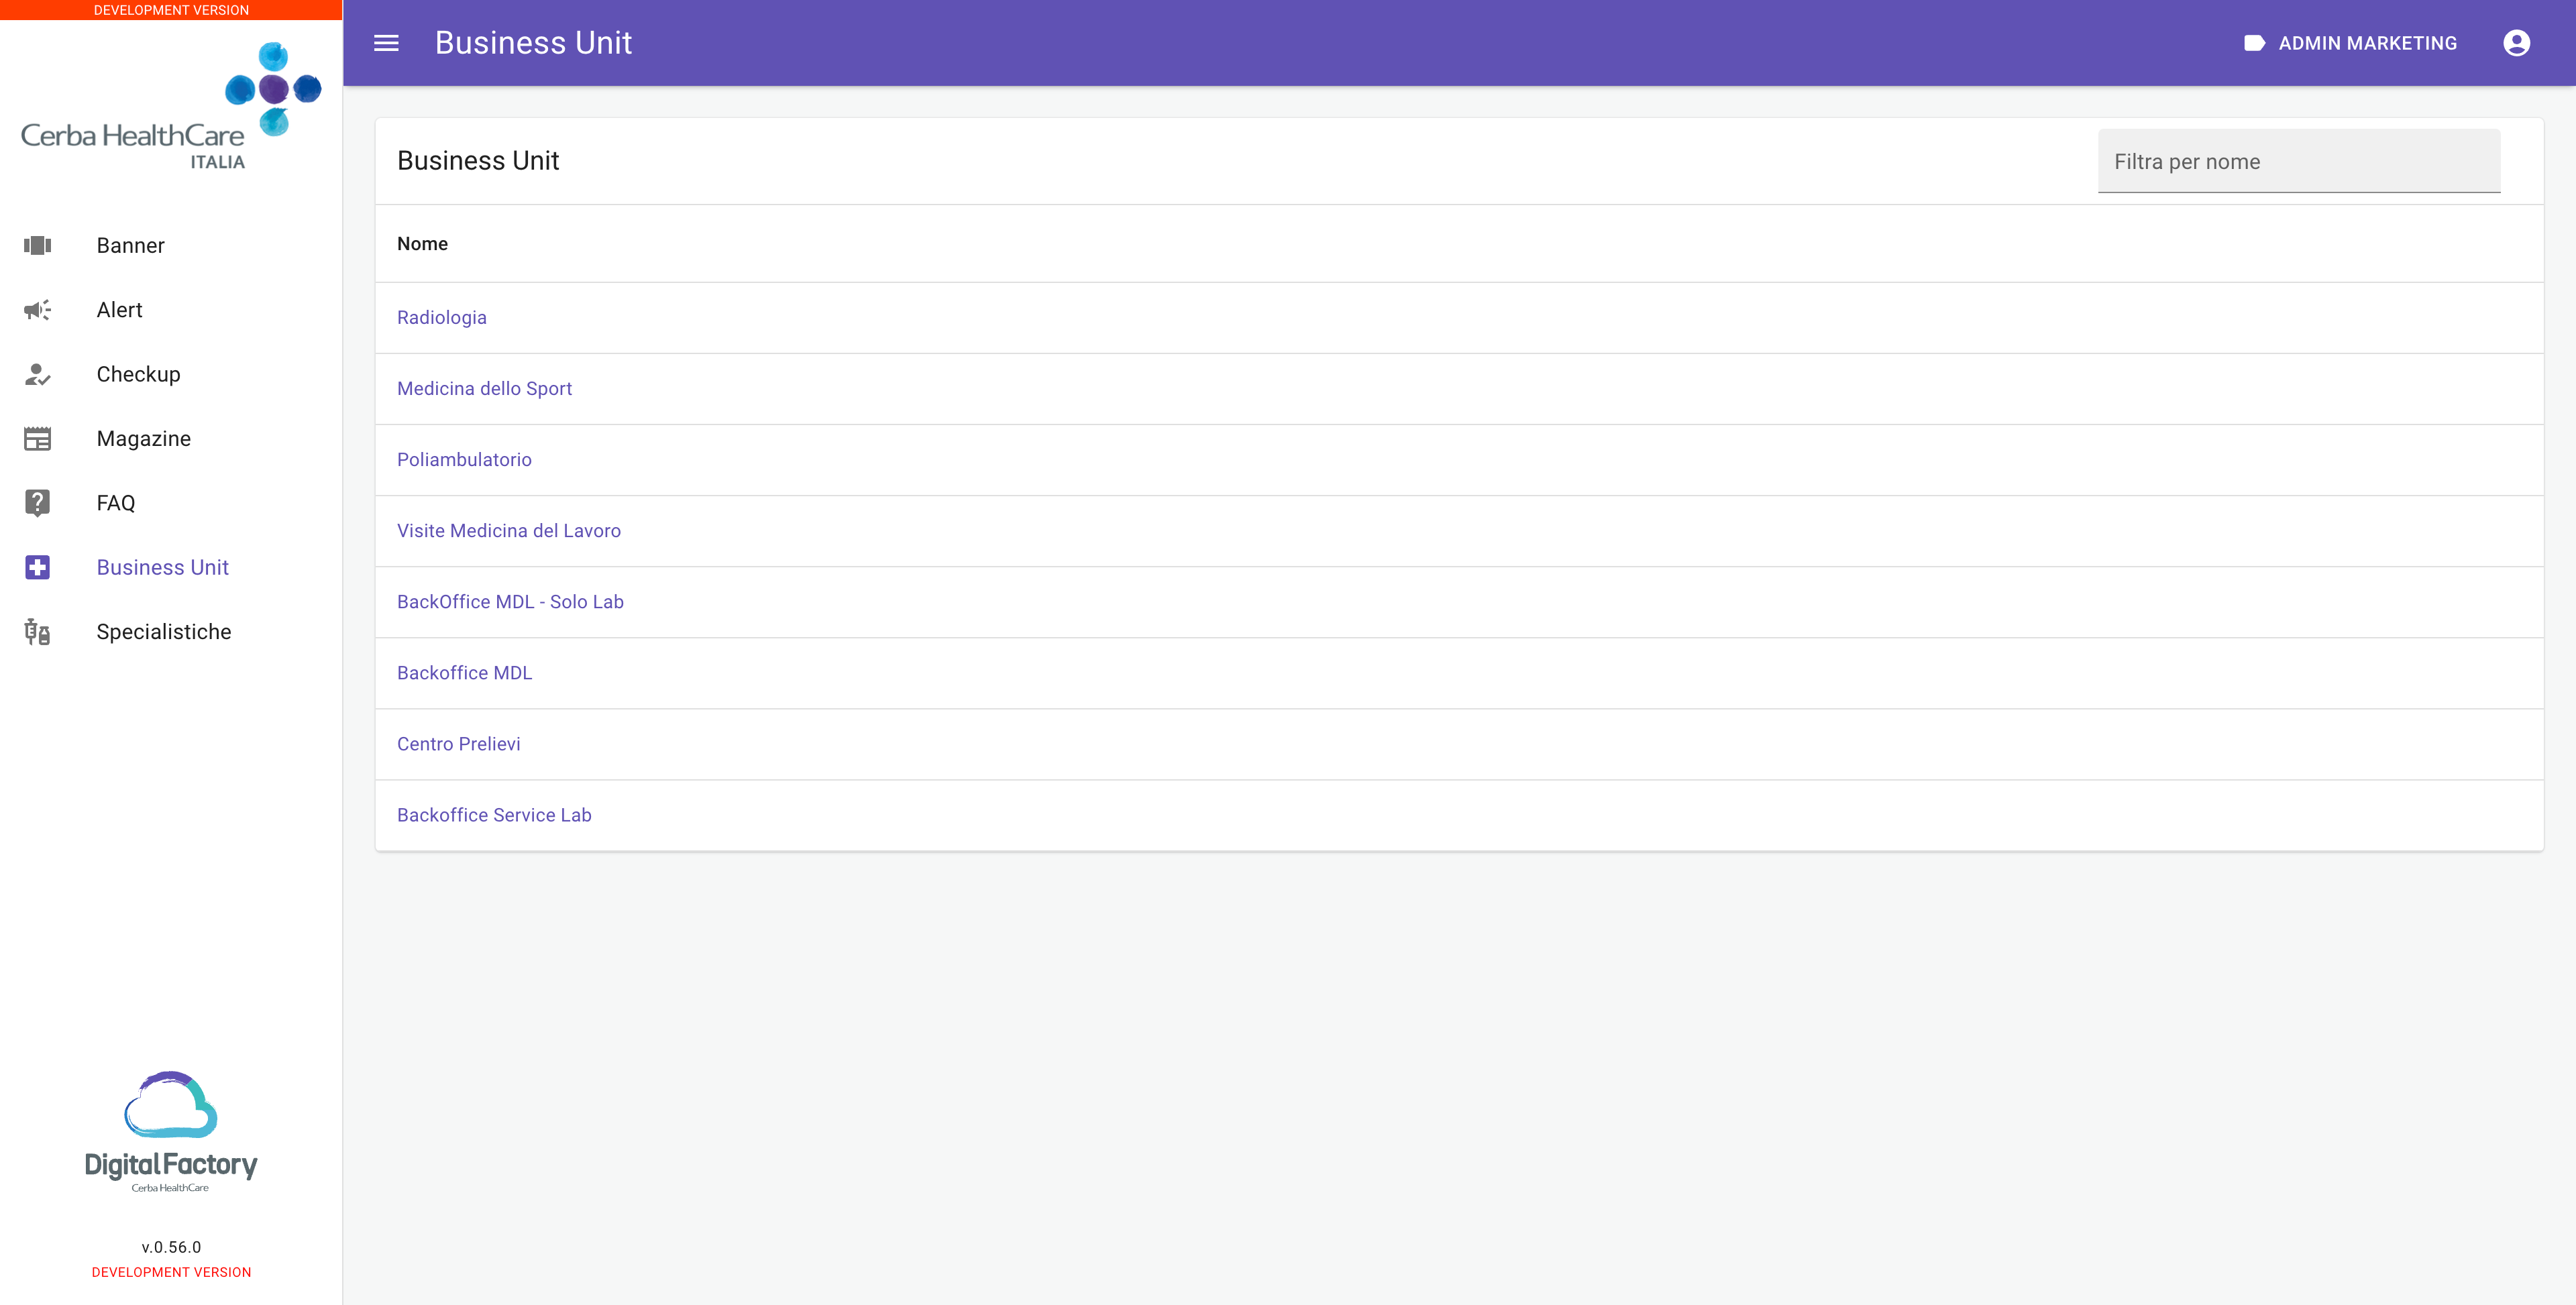
\includegraphics[width=0.75\textwidth]{images/capitolo5/f8_businessUnits/PageBusinessUnits_searchEmpty.png} 
    \caption{Tabella BU campo ricerca vuoto} 
    \label{fig:PageBusinessUnits_searchEmpty}
\end{figure}

\begin{figure}[H]
    \centering
    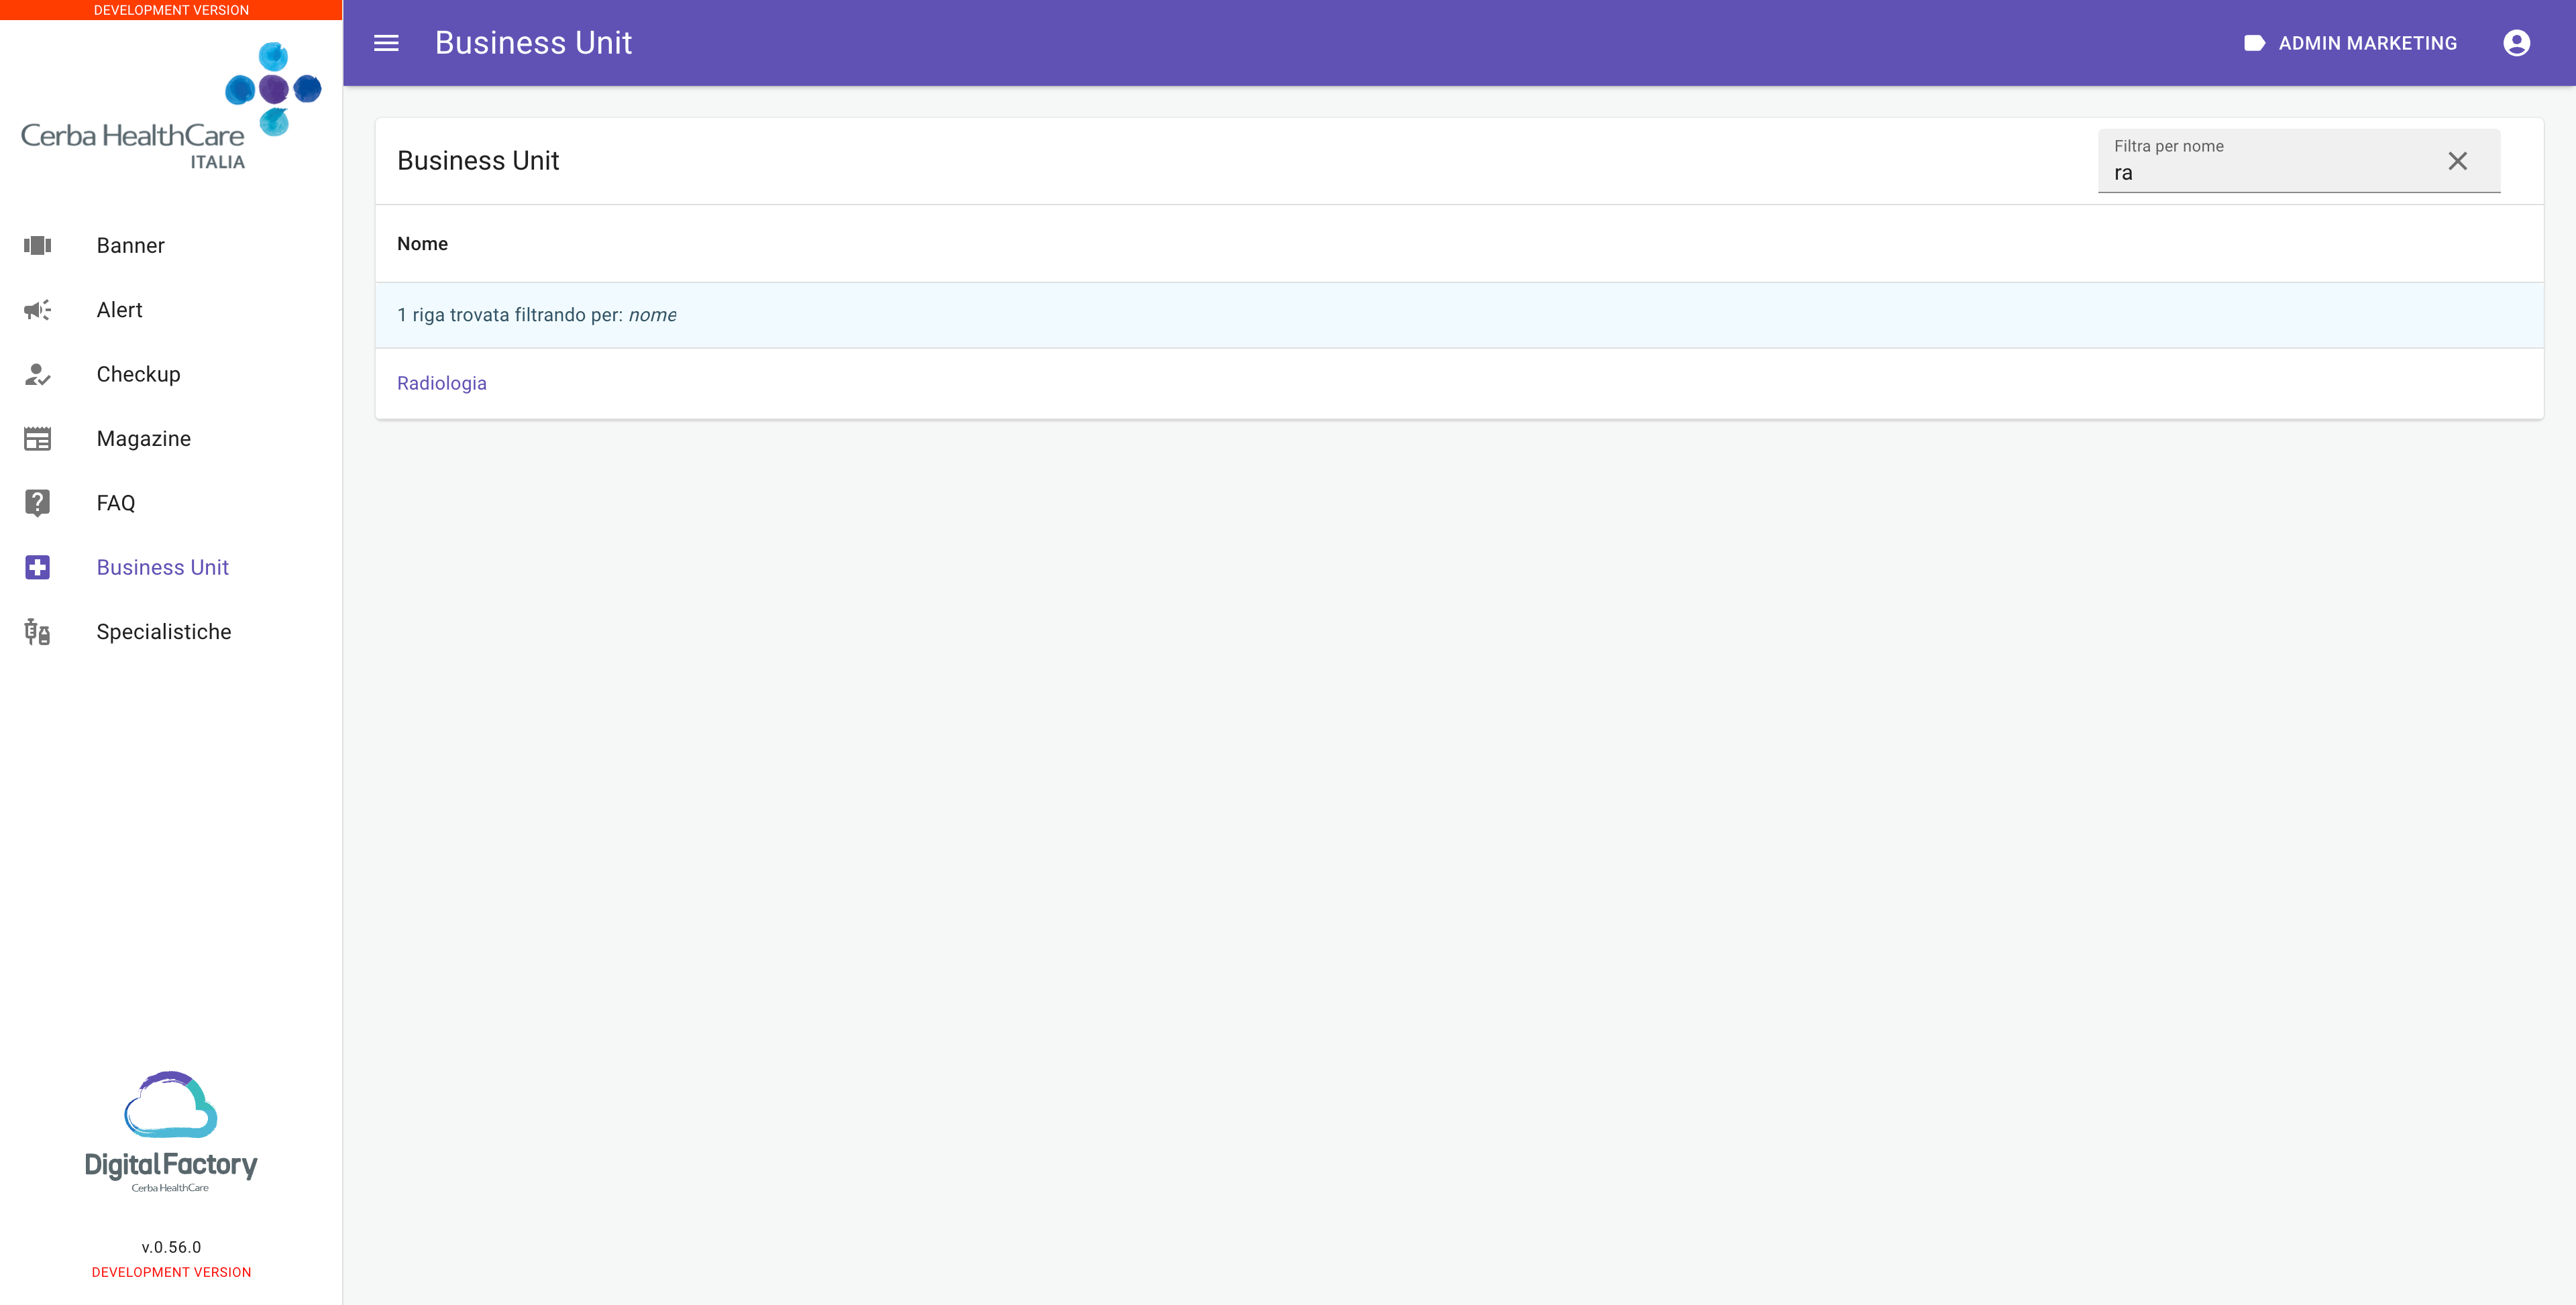
\includegraphics[width=0.75\textwidth]{images/capitolo5/f8_businessUnits/PageBusinessUnits_searchFilled.png} 
    \caption{Tabella BU campo ricerca riempito} 
    \label{fig:PageBusinessUnits_searchFilled}
\end{figure}

\begin{figure}[H]
    \centering
    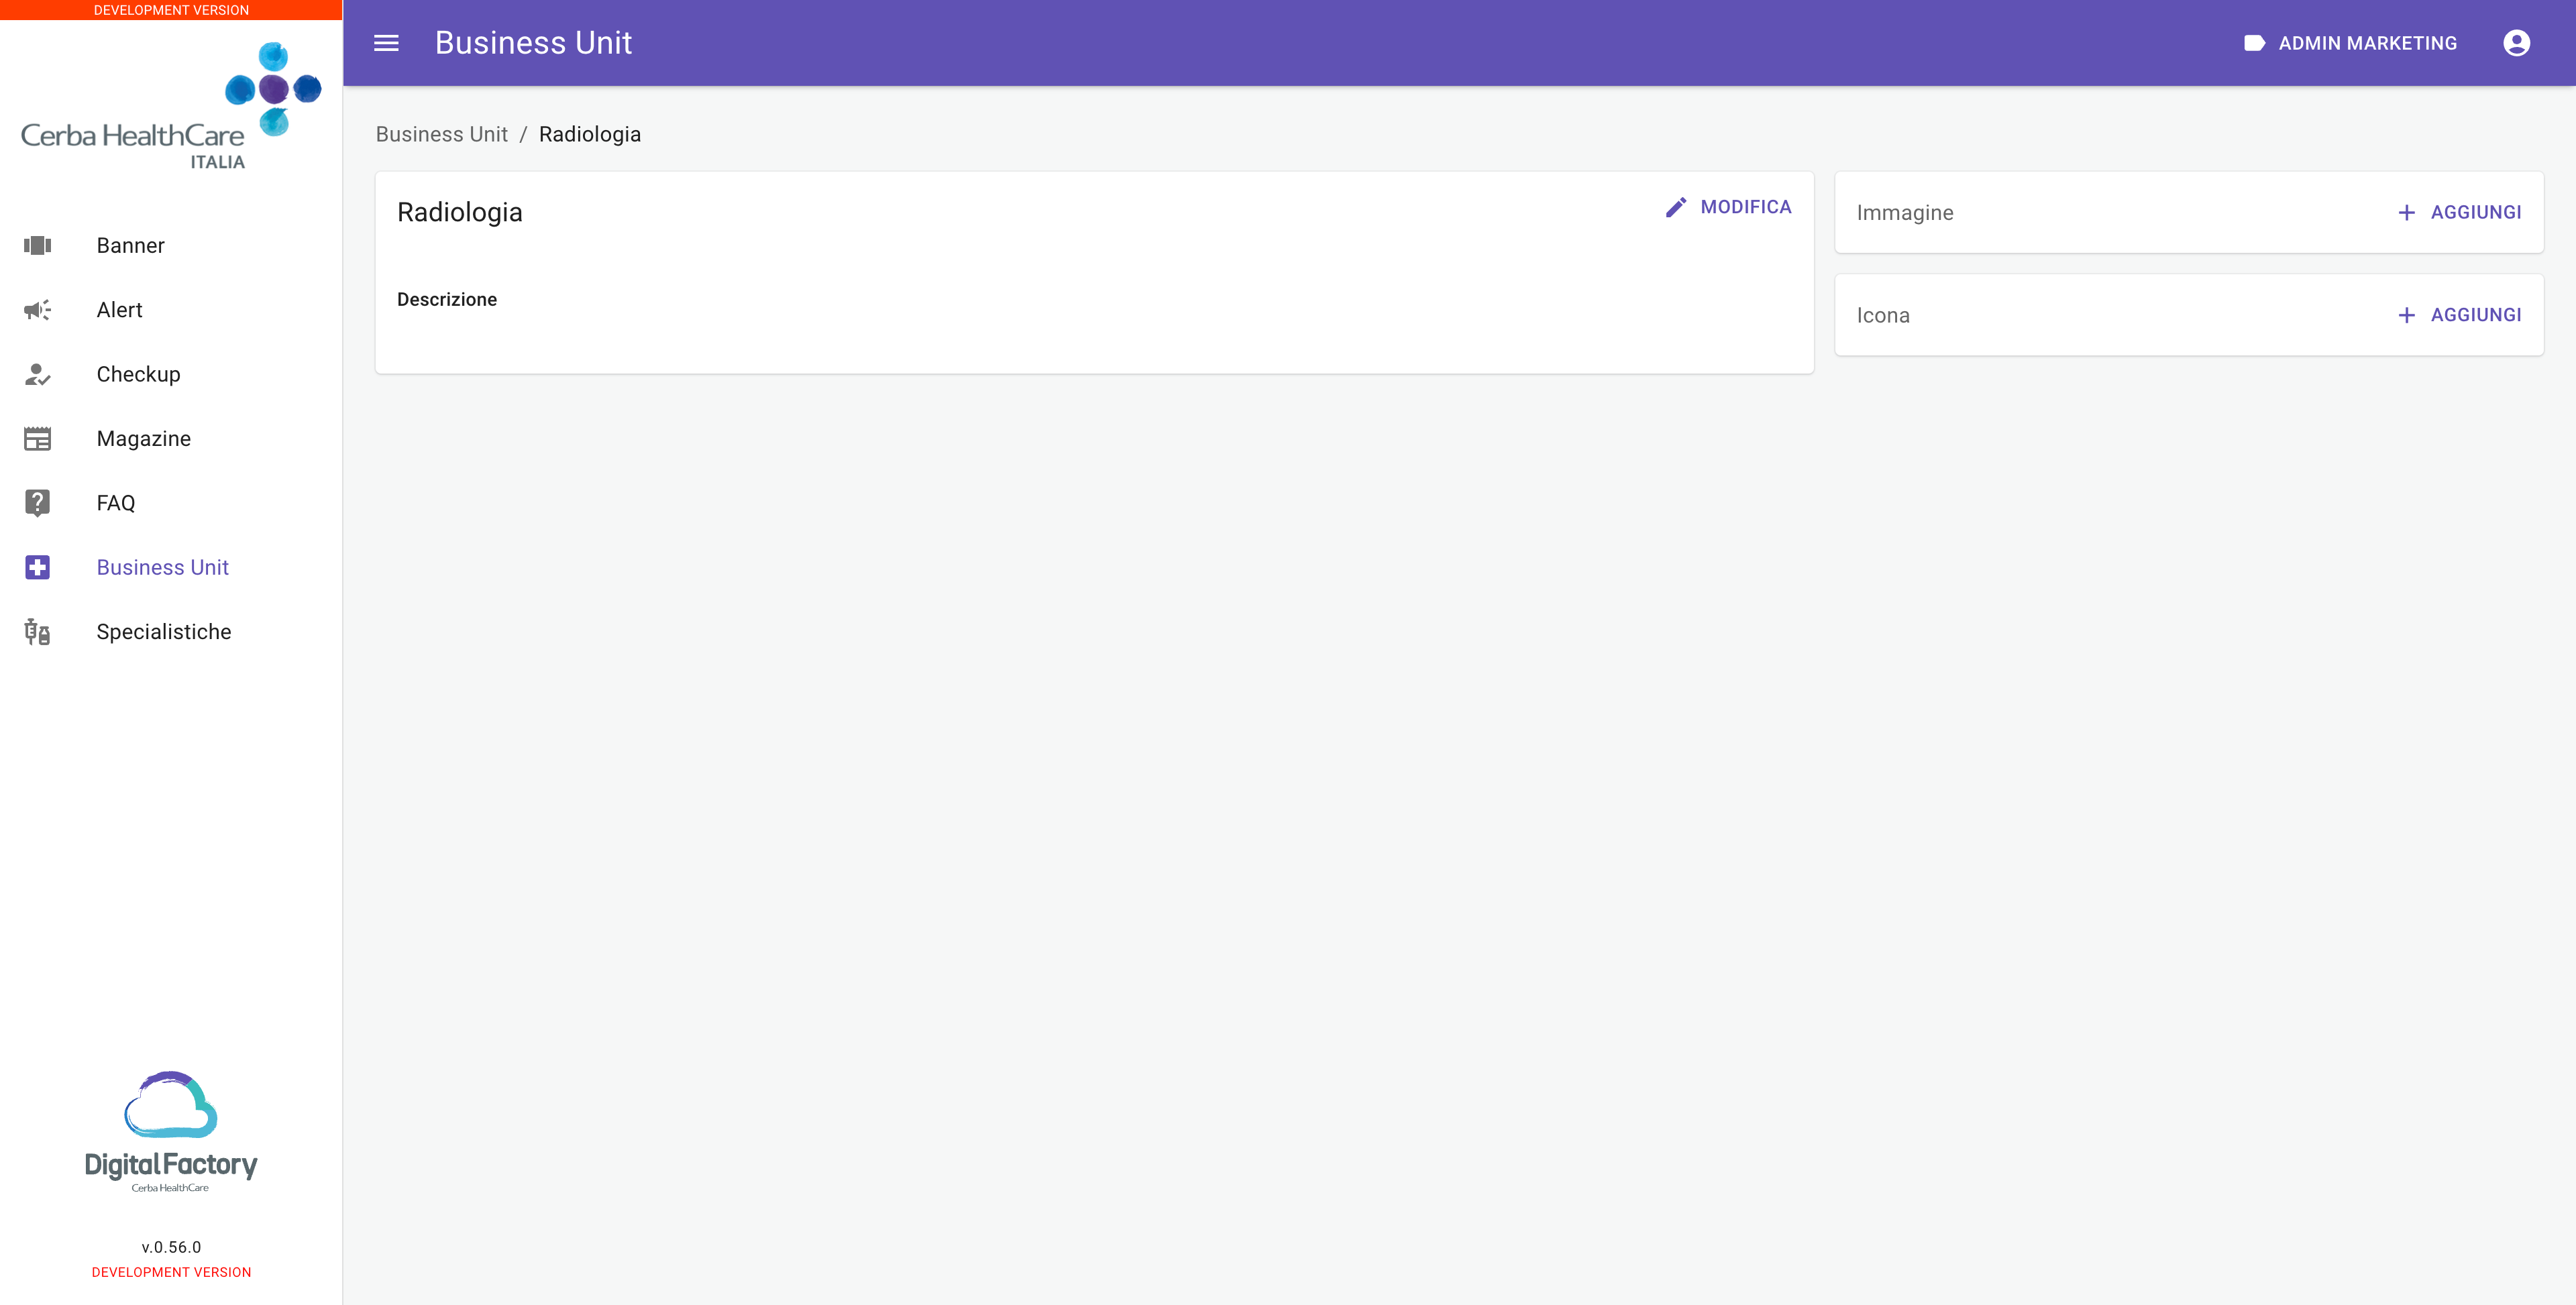
\includegraphics[width=0.75\textwidth]{images/capitolo5/f8_businessUnits/PageBusinessUnit.png} 
    \caption{Pagina dettaglio BU} 
    \label{fig:PageBusinessUnit}
\end{figure}

\begin{figure}[H]
    \centering
    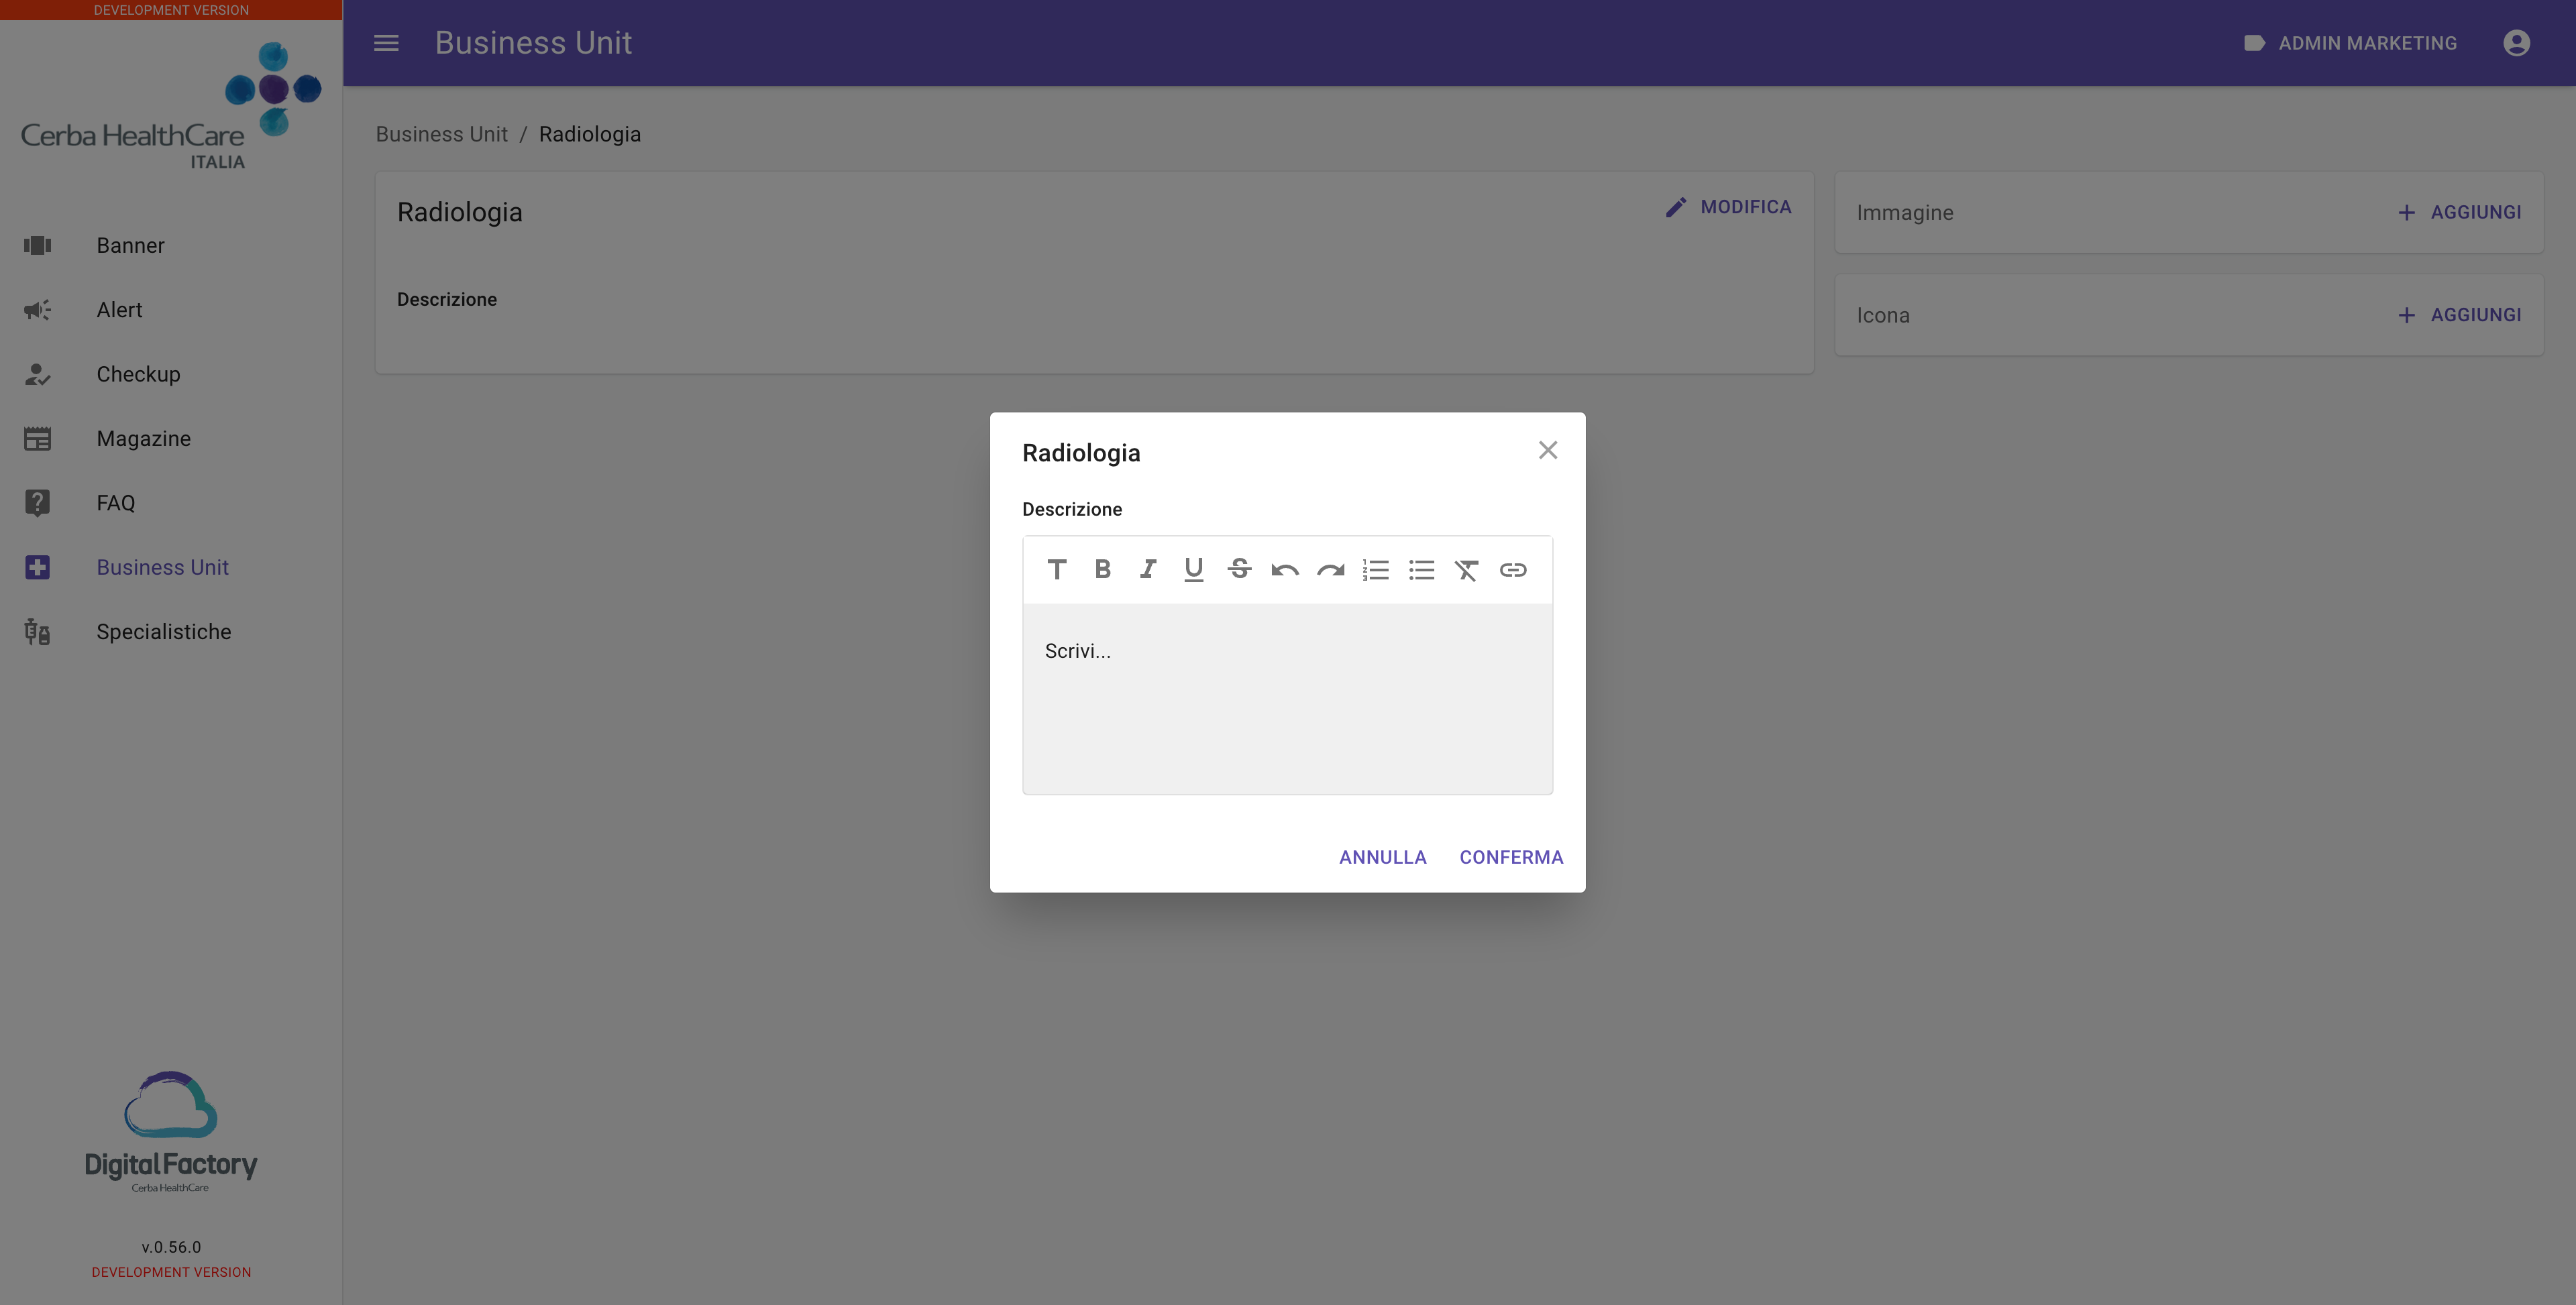
\includegraphics[width=0.75\textwidth]{images/capitolo5/f8_businessUnits/ModalBusinessUnit_edit.png} 
    \caption{Modale modifica descrizione BU} 
    \label{fig:ModalBusinessUnit_edit}
\end{figure}

\begin{figure}[H]
    \centering
    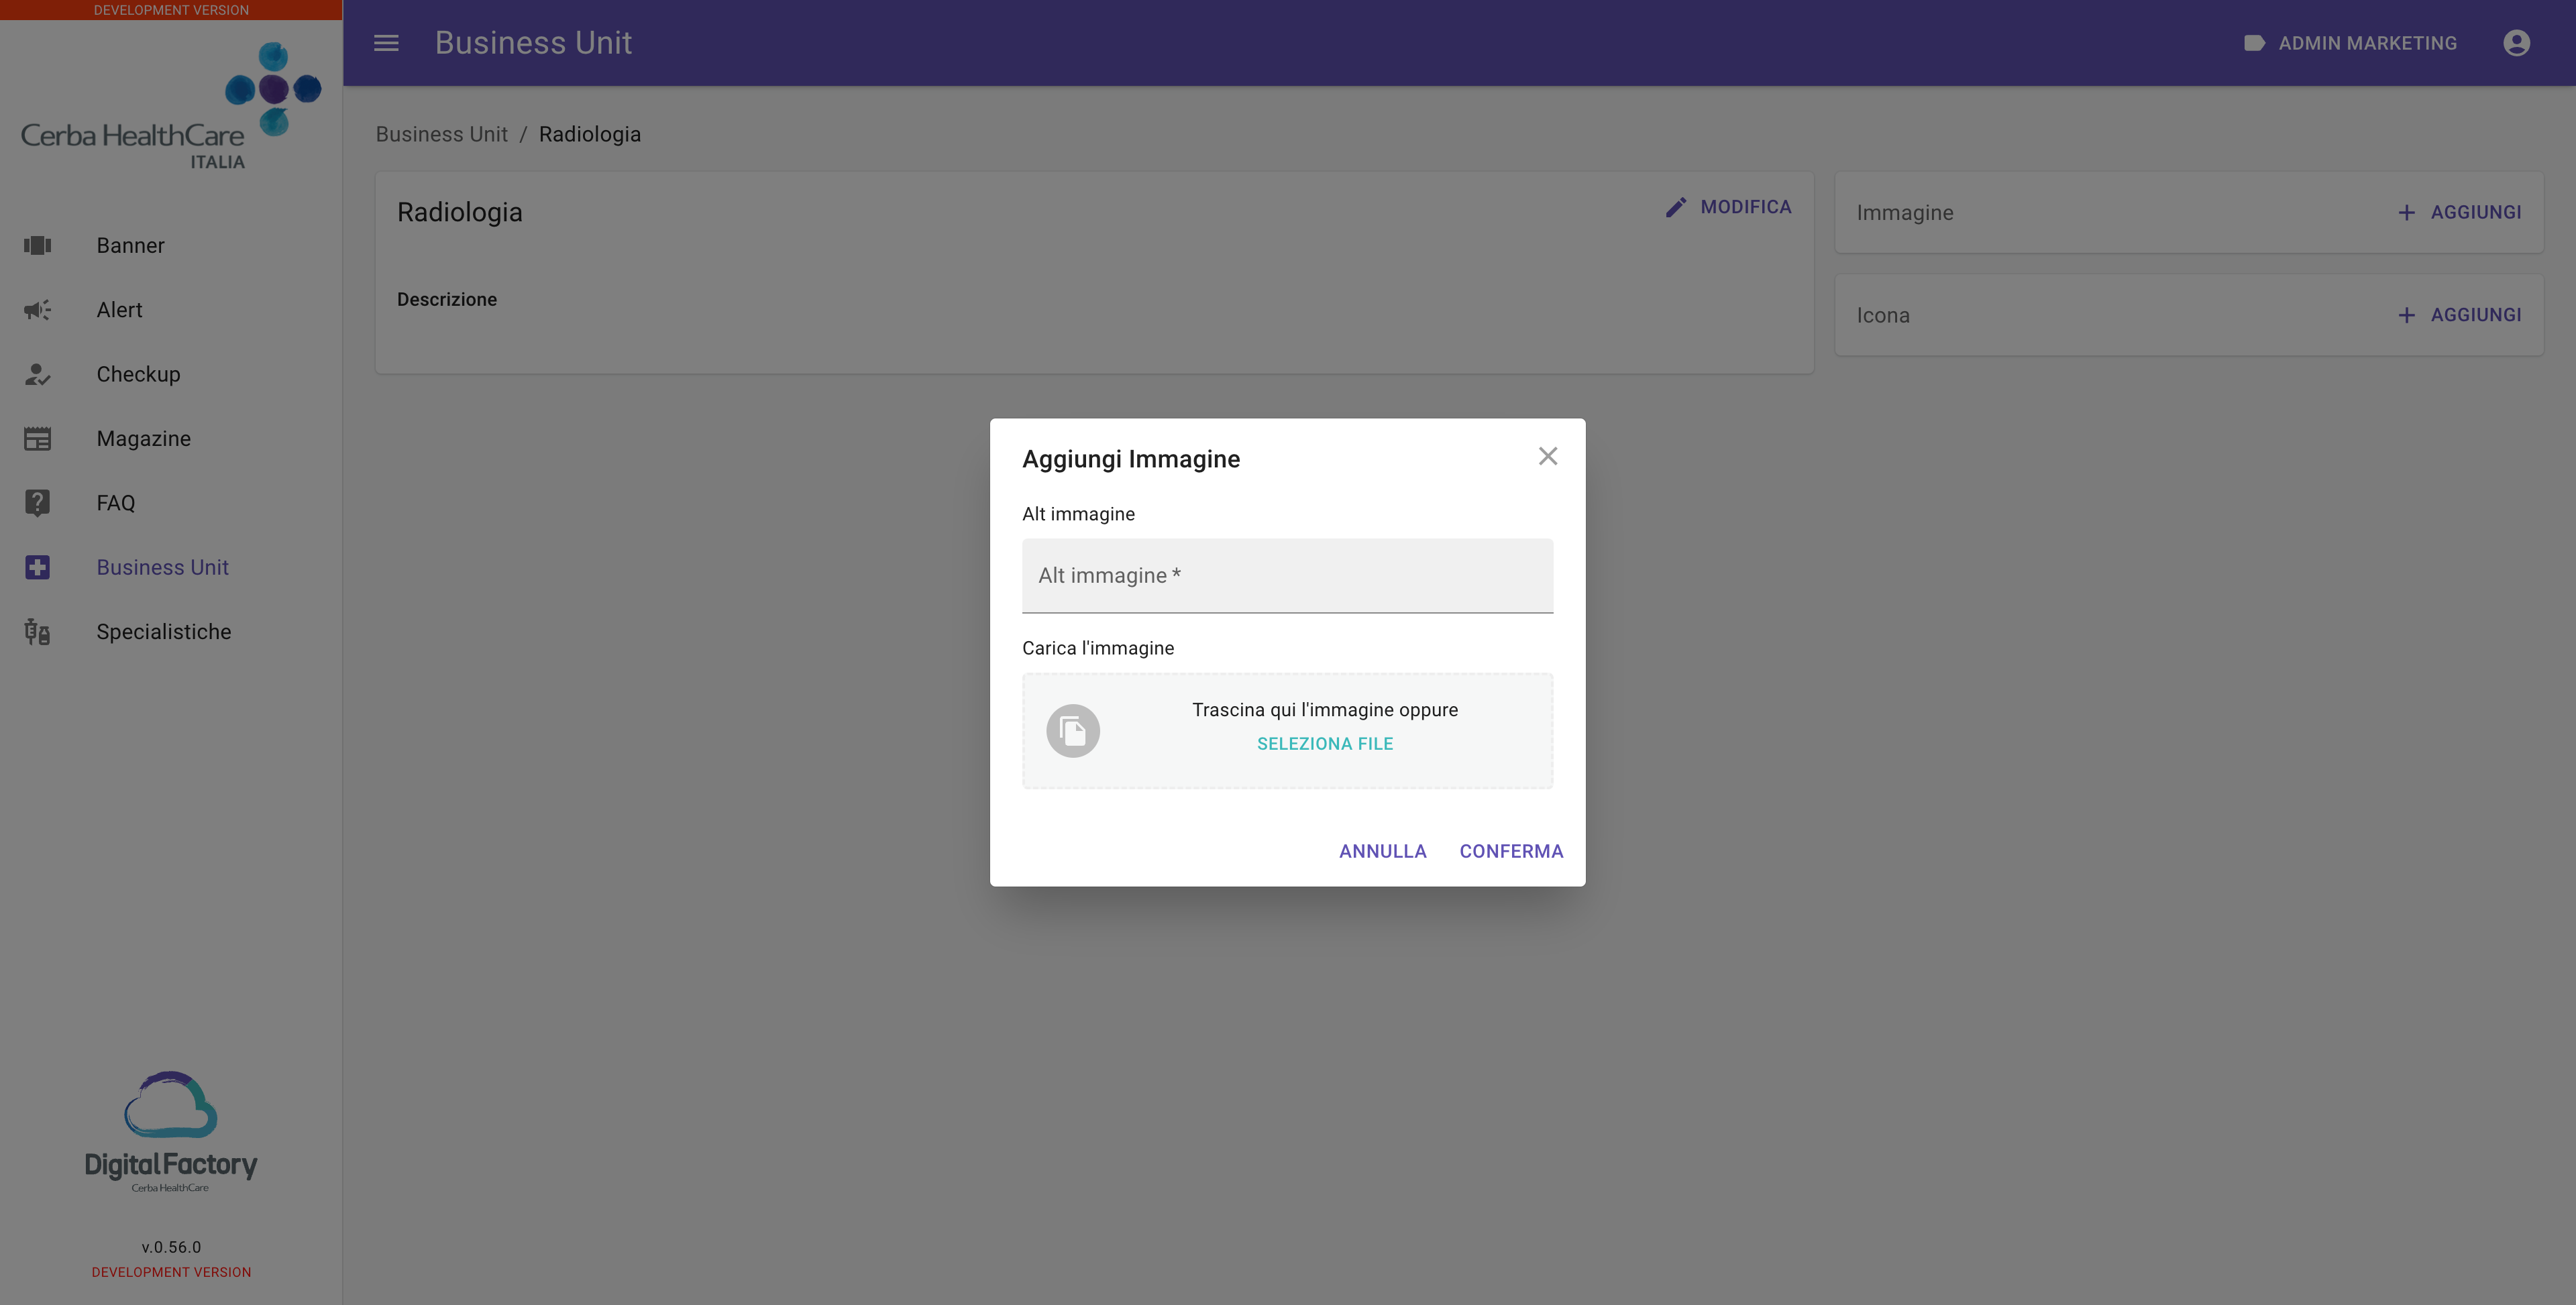
\includegraphics[width=0.75\textwidth]{images/capitolo5/f8_businessUnits/ModalBusinessUnit_createImage.png} 
    \caption{Modale aggiunta immagine BU} 
    \label{fig:ModalBusinessUnit_createImage}
\end{figure}

\begin{figure}[H]
    \centering
    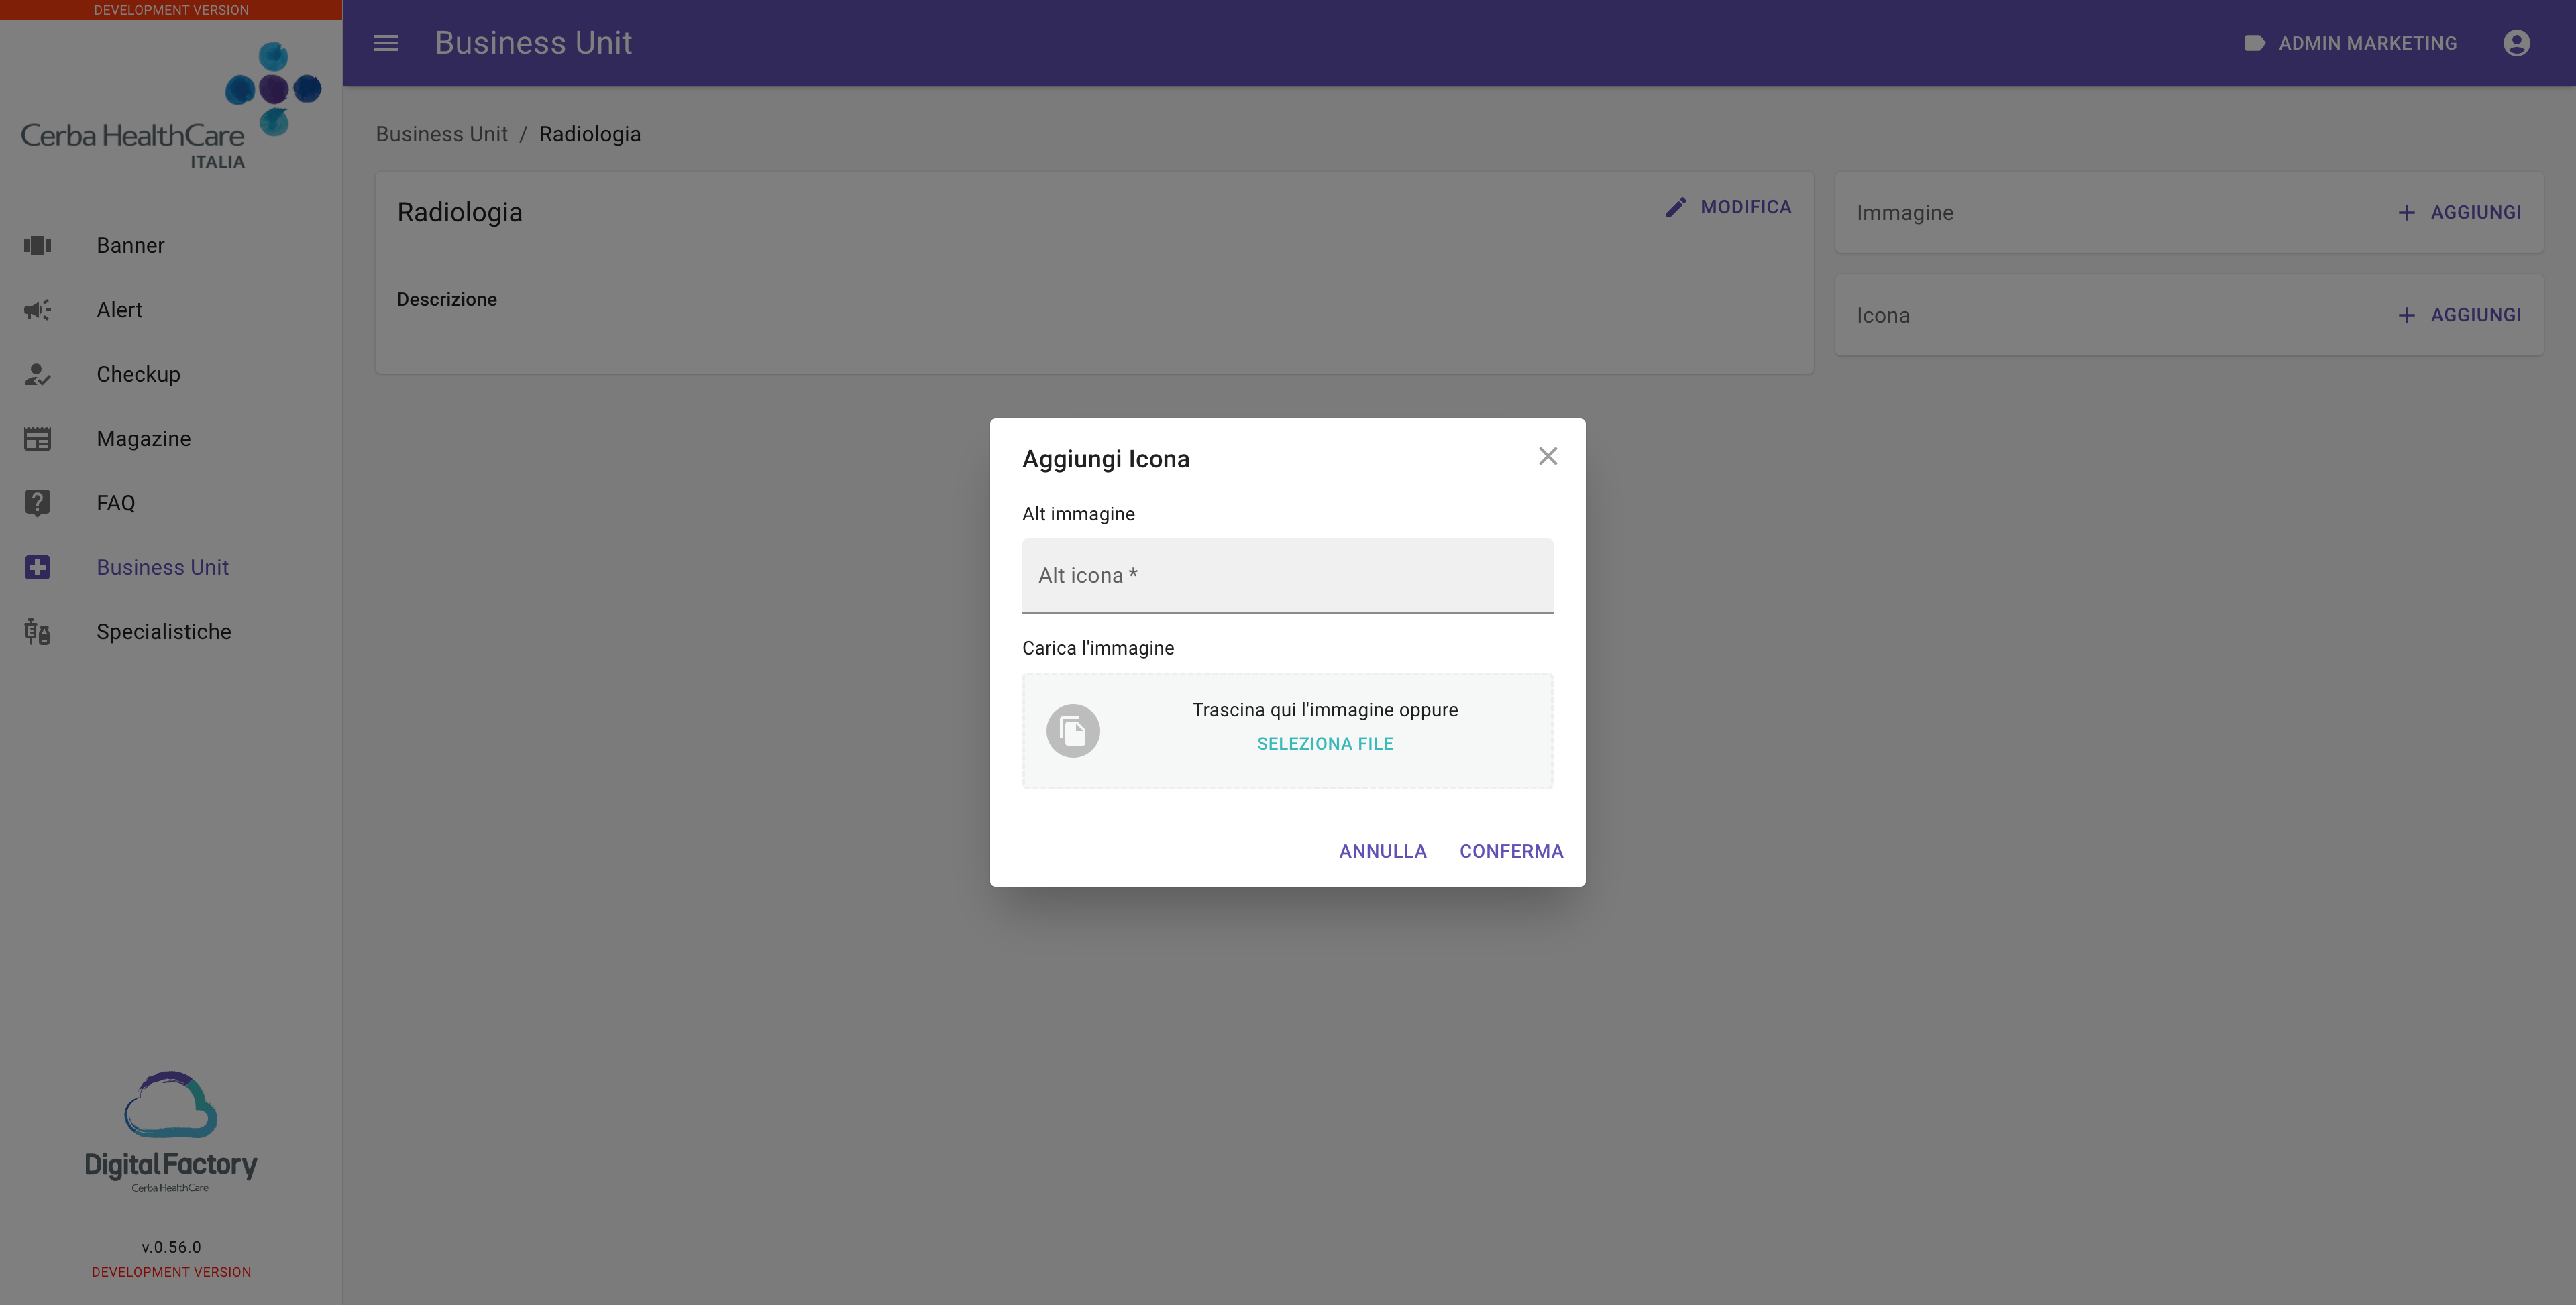
\includegraphics[width=0.75\textwidth]{images/capitolo5/f8_businessUnits/ModalBusinessUnit_createIcon.png} 
    \caption{Modale aggiunta icona BU} 
    \label{fig:ModalBusinessUnit_createIcon}
\end{figure}

\begin{figure}[H]
    \centering
    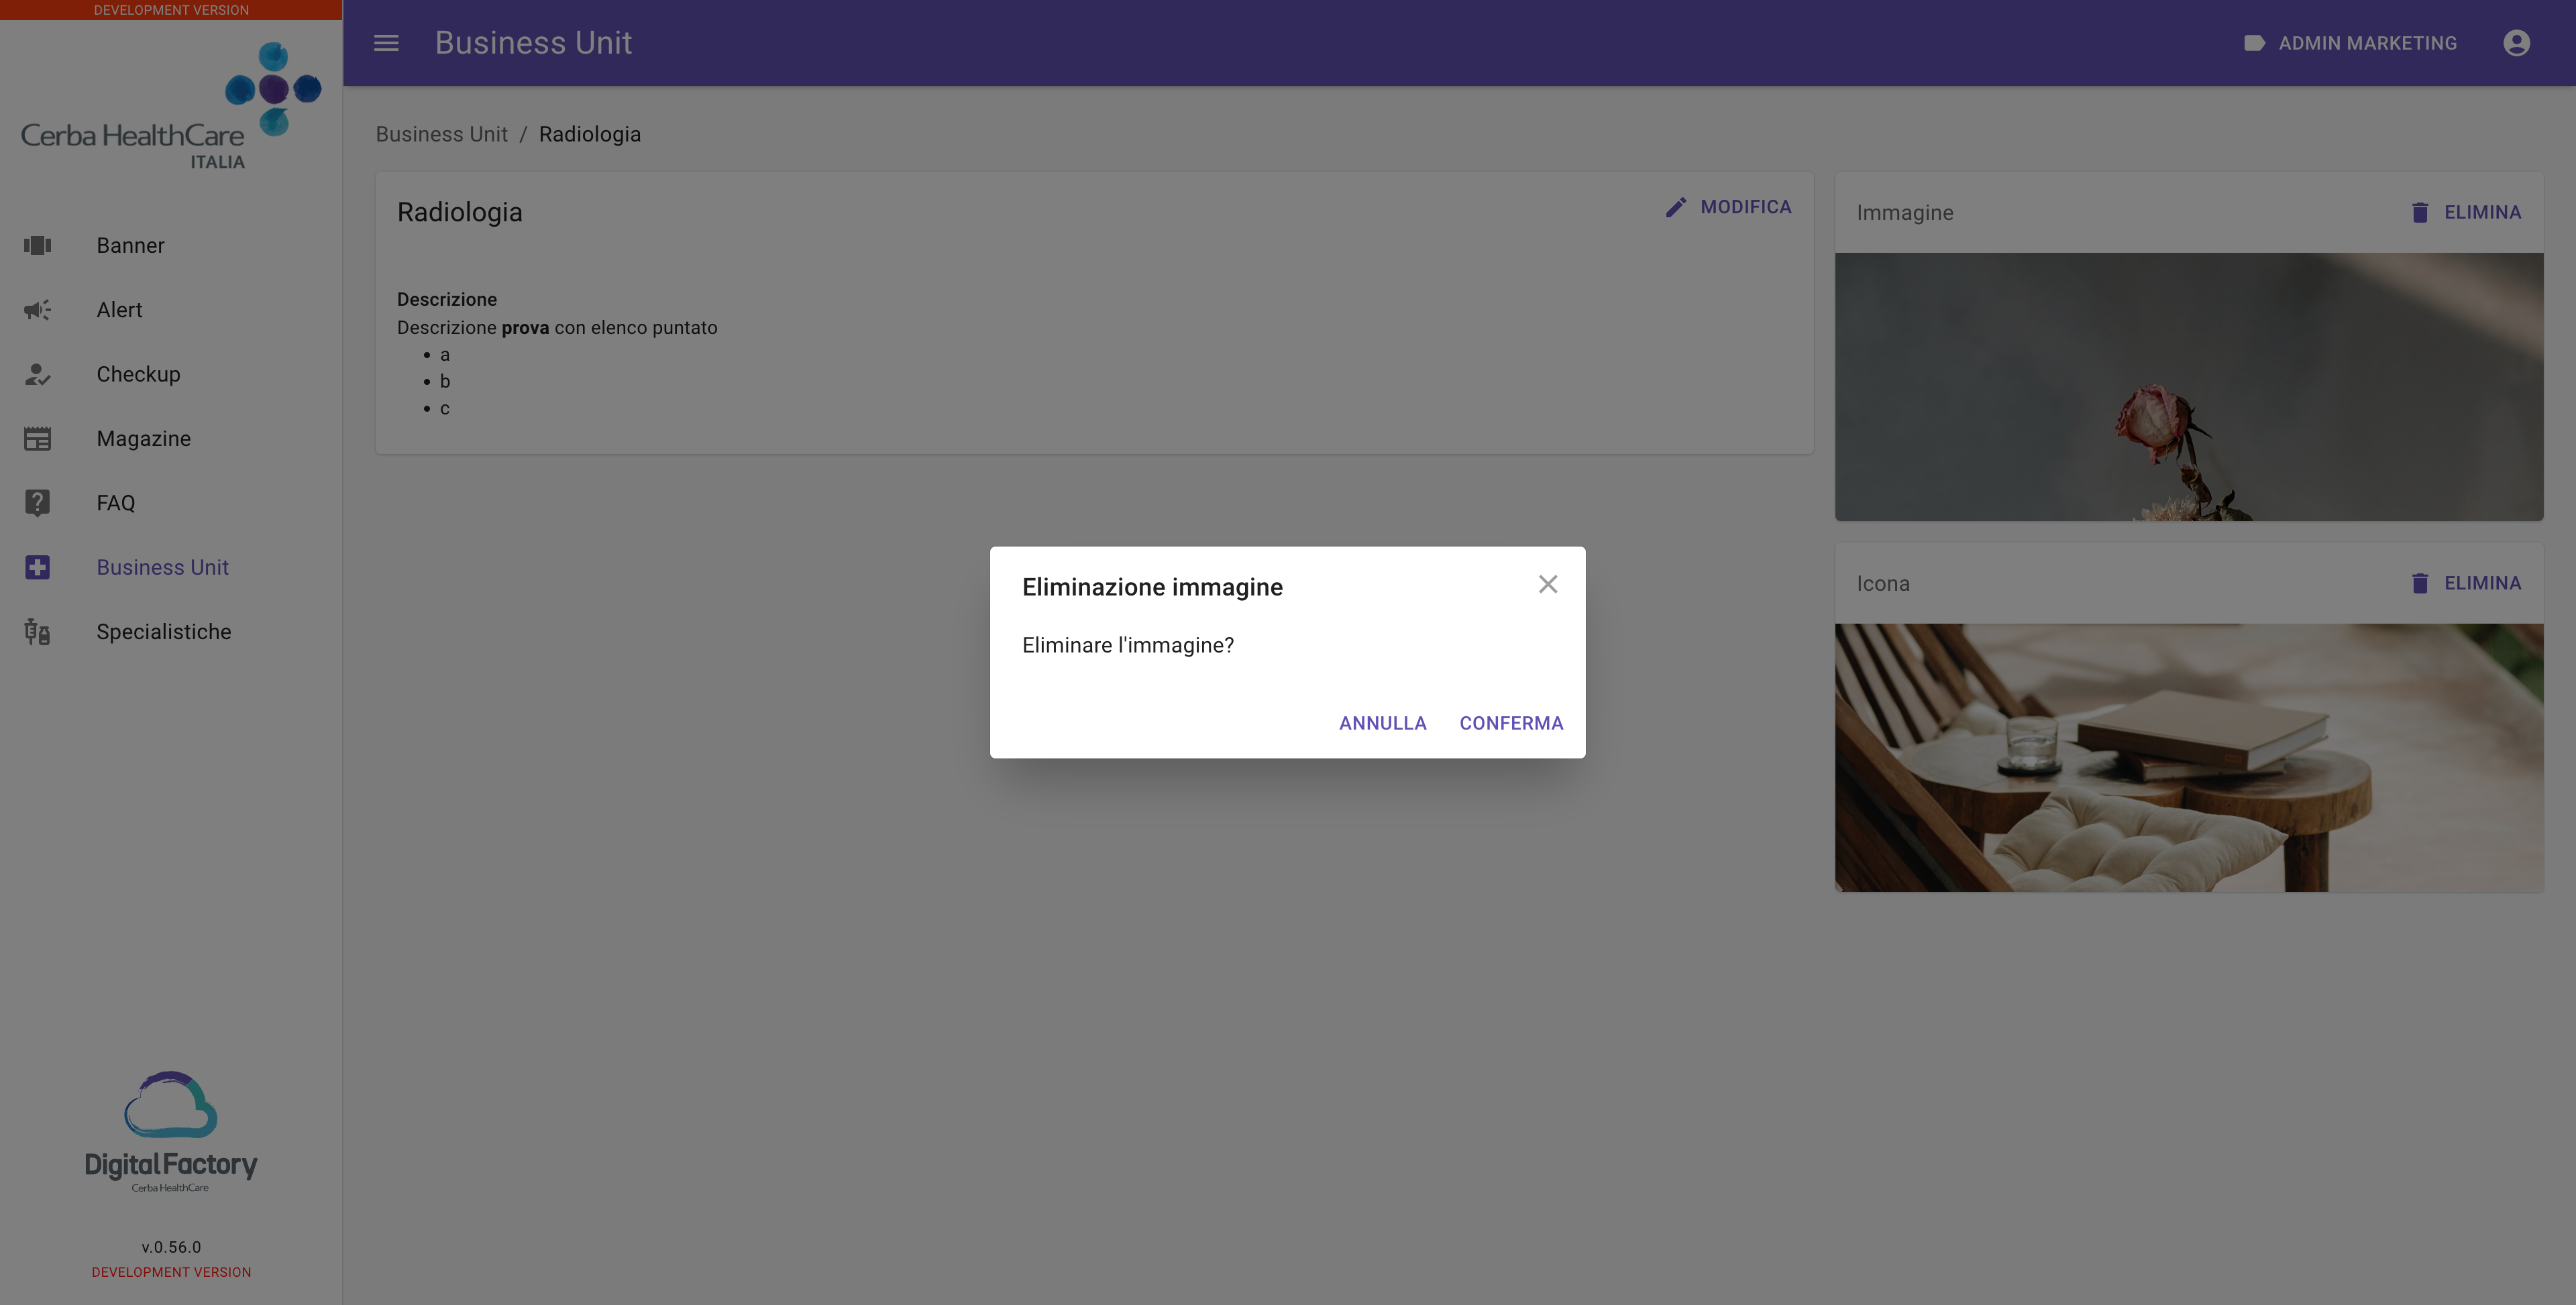
\includegraphics[width=0.75\textwidth]{images/capitolo5/f8_businessUnits/ModalBusinessUnit_deleteImage.png} 
    \caption{Modale eliminazione immagine BU} 
    \label{fig:ModalBusinessUnit_deleteImage}
\end{figure}

\begin{figure}[H]
    \centering
    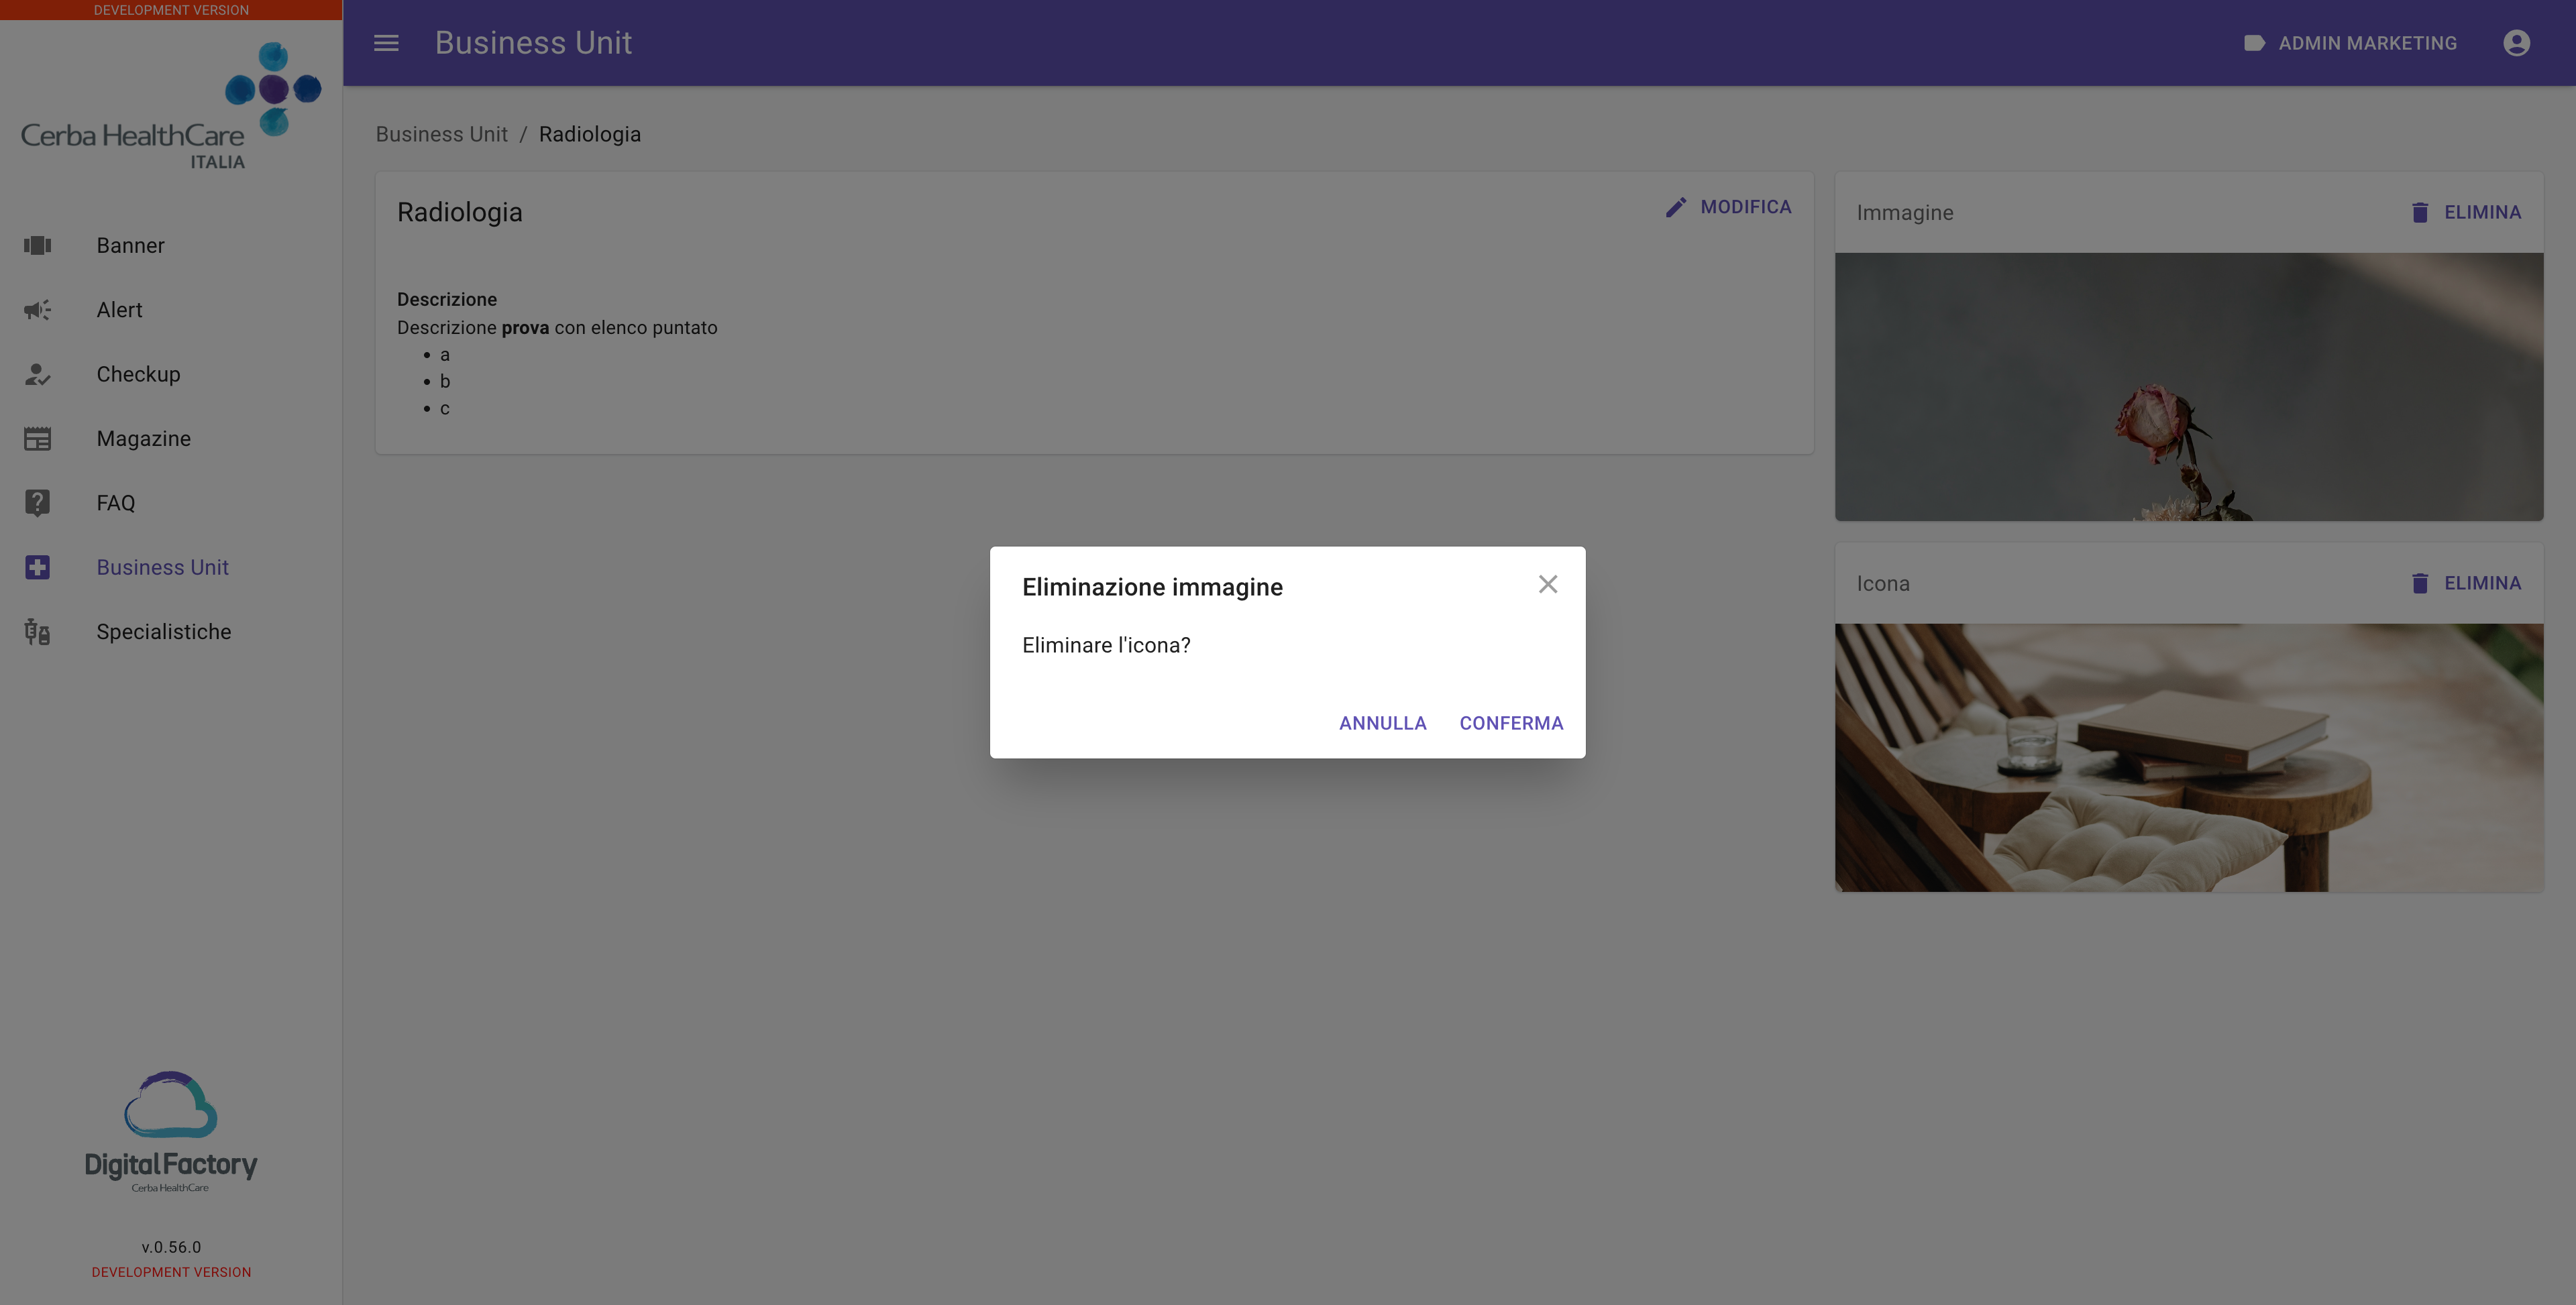
\includegraphics[width=0.75\textwidth]{images/capitolo5/f8_businessUnits/ModalBusinessUnit_deleteIcon.png} 
    \caption{Modale eliminazione icona BU} 
    \label{fig:ModalBusinessUnit_deleteIcon}
\end{figure}

\subsection{F9: “Specialistiche”}
\subparagraph{Requisiti}
Aggiungere la sezione “Specialistiche” fra quelle previste per il ruolo utente \textit{marketing admin}.\\
Al suo interno, una tabella deve mostrare le specialistiche esistenti in una lista semplice e riportarne la proprietà “Nome”.\\
L'\textit{header} della tabella delle specialistiche deve essere dotato di un campo di ricerca. Questo deve essere in grado di filtrare per nome e posizionato all'estrema destra dell'\textit{header} della tabella.\\
Ogni specialistica deve essere dotata di una pagina di dettaglio alla quale si accede cliccando sul link posto in concomitanza del nome. Qui, deve essere possibile modificare e visualizzare la descrizione, proprietà che deve poter essere formattata; sempre all'interno della pagina di dettaglio, si devono poter aggiungere, visualizzare ed eliminare un'immagine e un'icona.

\subsection{F10: “Posizoni aperte”}
\subparagraph{Requisiti}
Aggiungere la sezione “Posizioni aperte” fra quelle previste per il ruolo utente \textit{hr admin}.\\
Al suo interno, una tabella deve mostrare le posizioni aperte esistenti in una lista semplice e riportarne la proprietà “Città”, “Data”, “Area” e “Nome”.\\
Deve essere possibile aggiungere o eliminare una posizione.\\
L'\textit{header} della tabella delle posizioni aperte deve essere dotato di un campo di ricerca. Questo deve essere in grado di filtrare per nome e posizionato posizionato alla sinistra del bottone per l'aggiunta di una nuova posizione.\\
Ogni posizione aperta deve essere dotata di una pagina di dettaglio alla quale si accede cliccando sul link posto in concomitanza del nome. Qui, deve essere possibile modificare e visualizzare i campi delle informazioni, e solamente per la proprietà “Descrizione” deve essere fornita la possibilità di formattazione.

\paragraph{\textit{Output} grafico}
\begin{figure}[H]
    \centering
    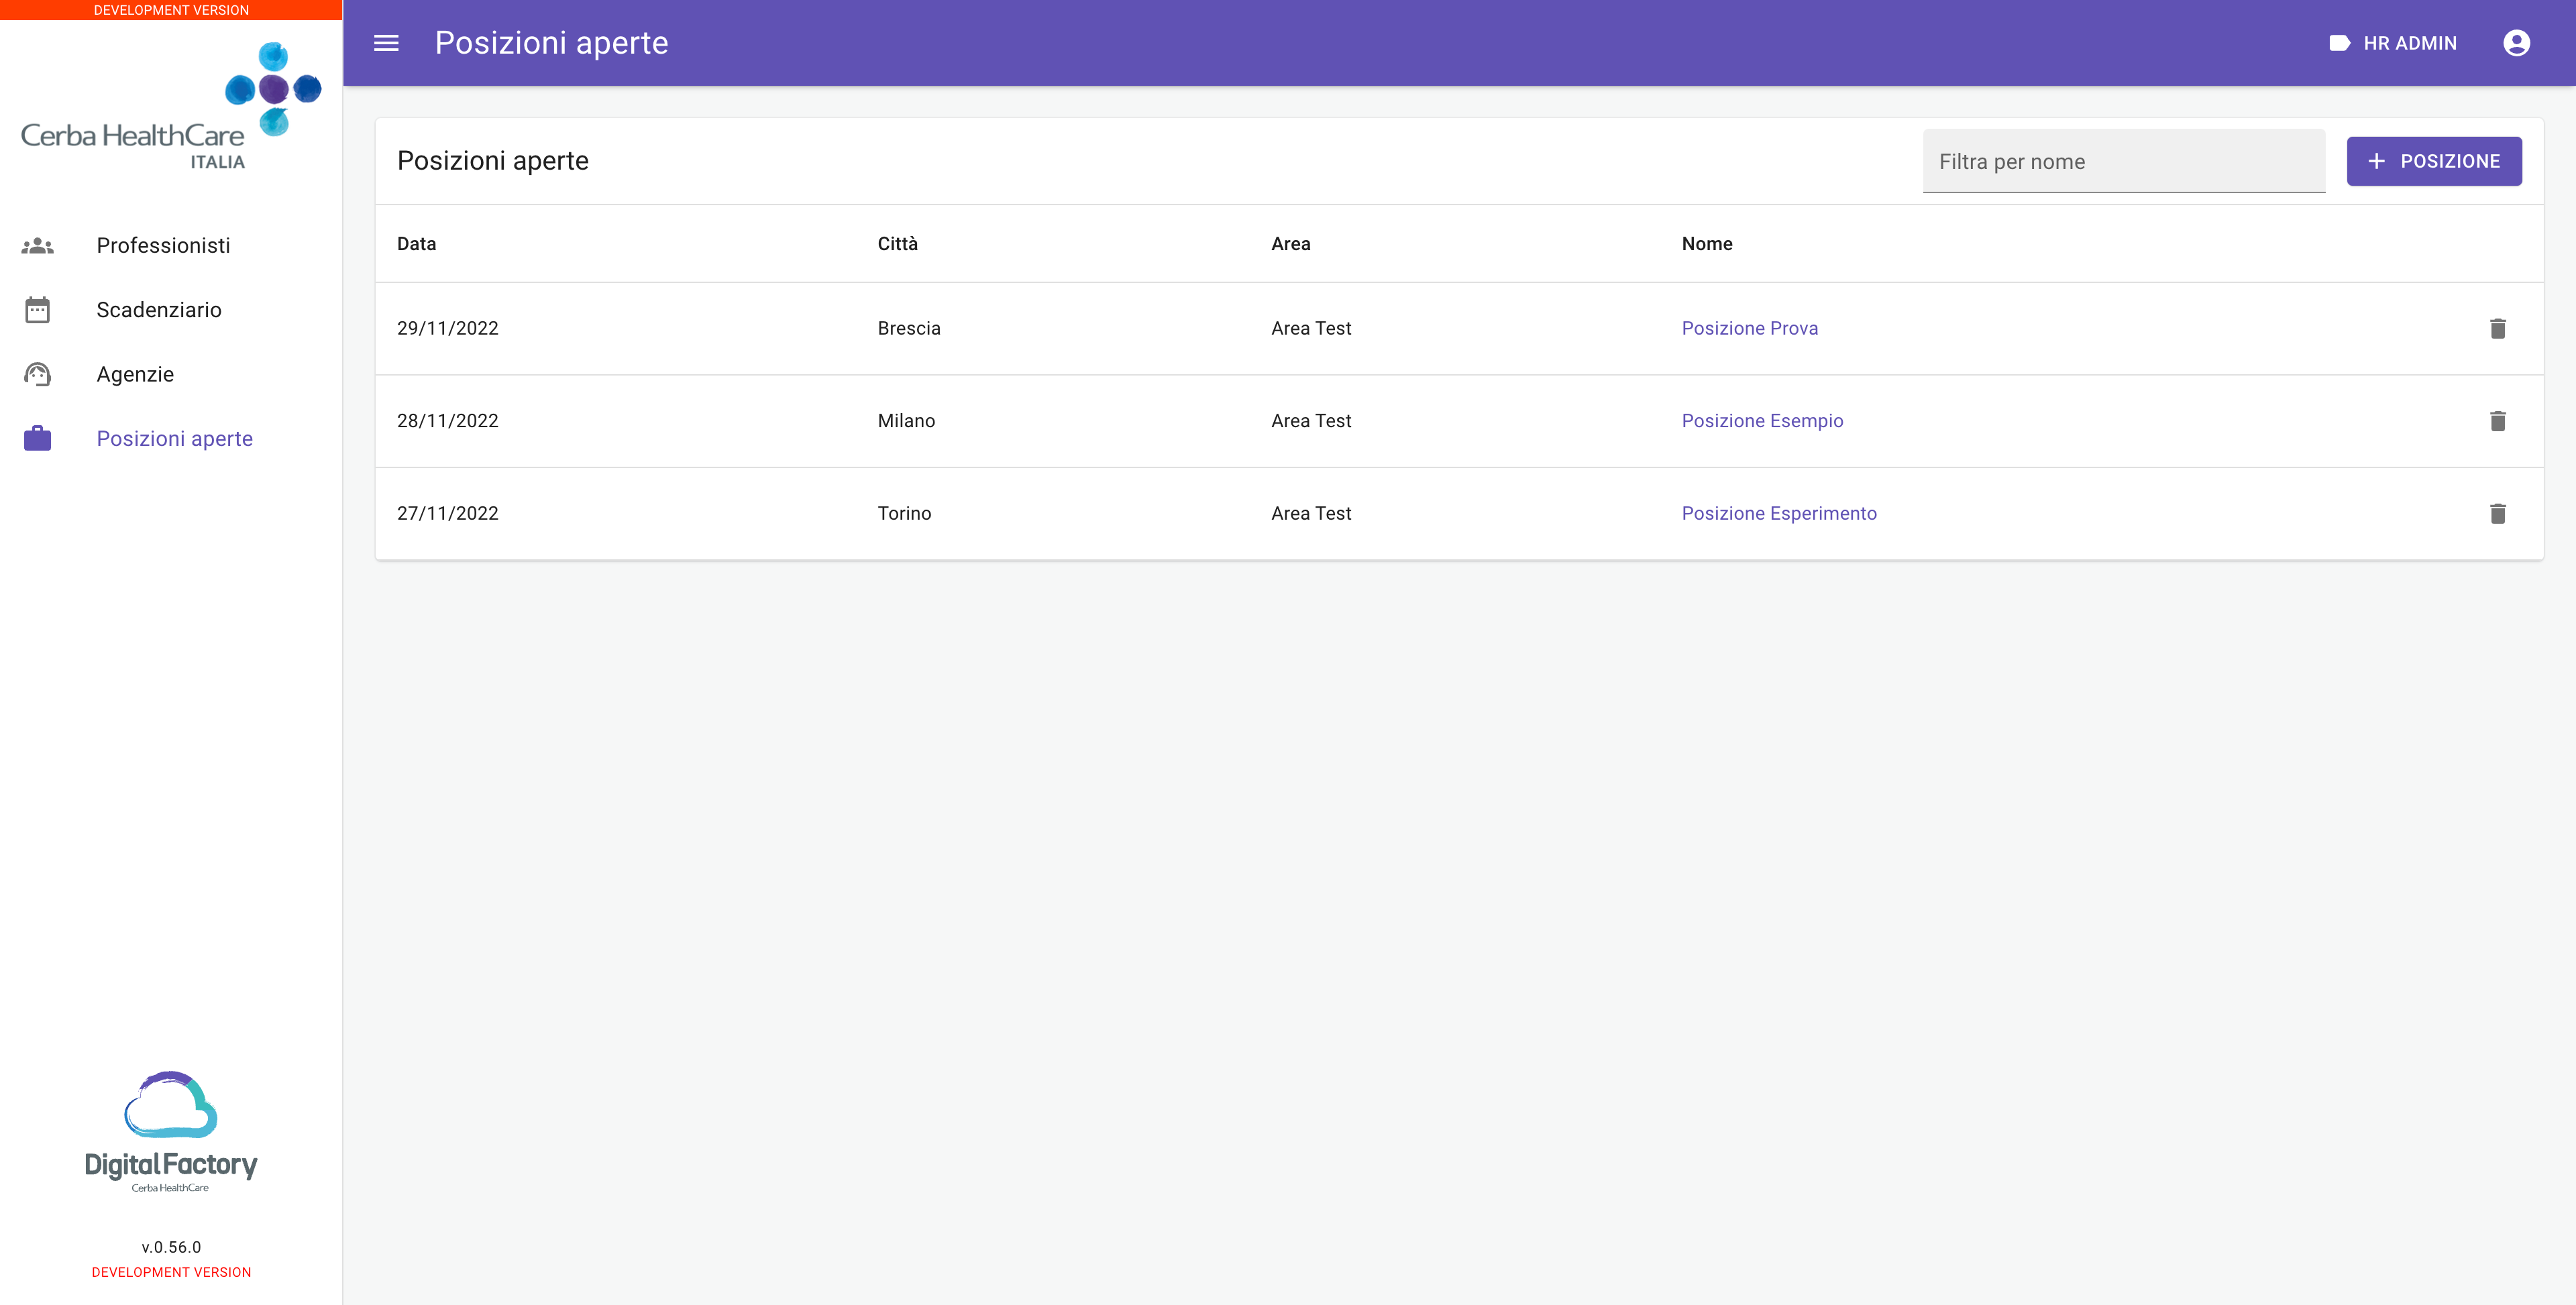
\includegraphics[width=0.75\textwidth]{images/capitolo5/f10_jobOpenPositions/PageJobOpenPositions_searchEmpty.png} 
    \caption{Tabella posizioni aperte campo ricerca vuoto} 
    \label{fig:PageJobOpenPositions_searchEmpty}
\end{figure}

\begin{figure}[H]
    \centering
    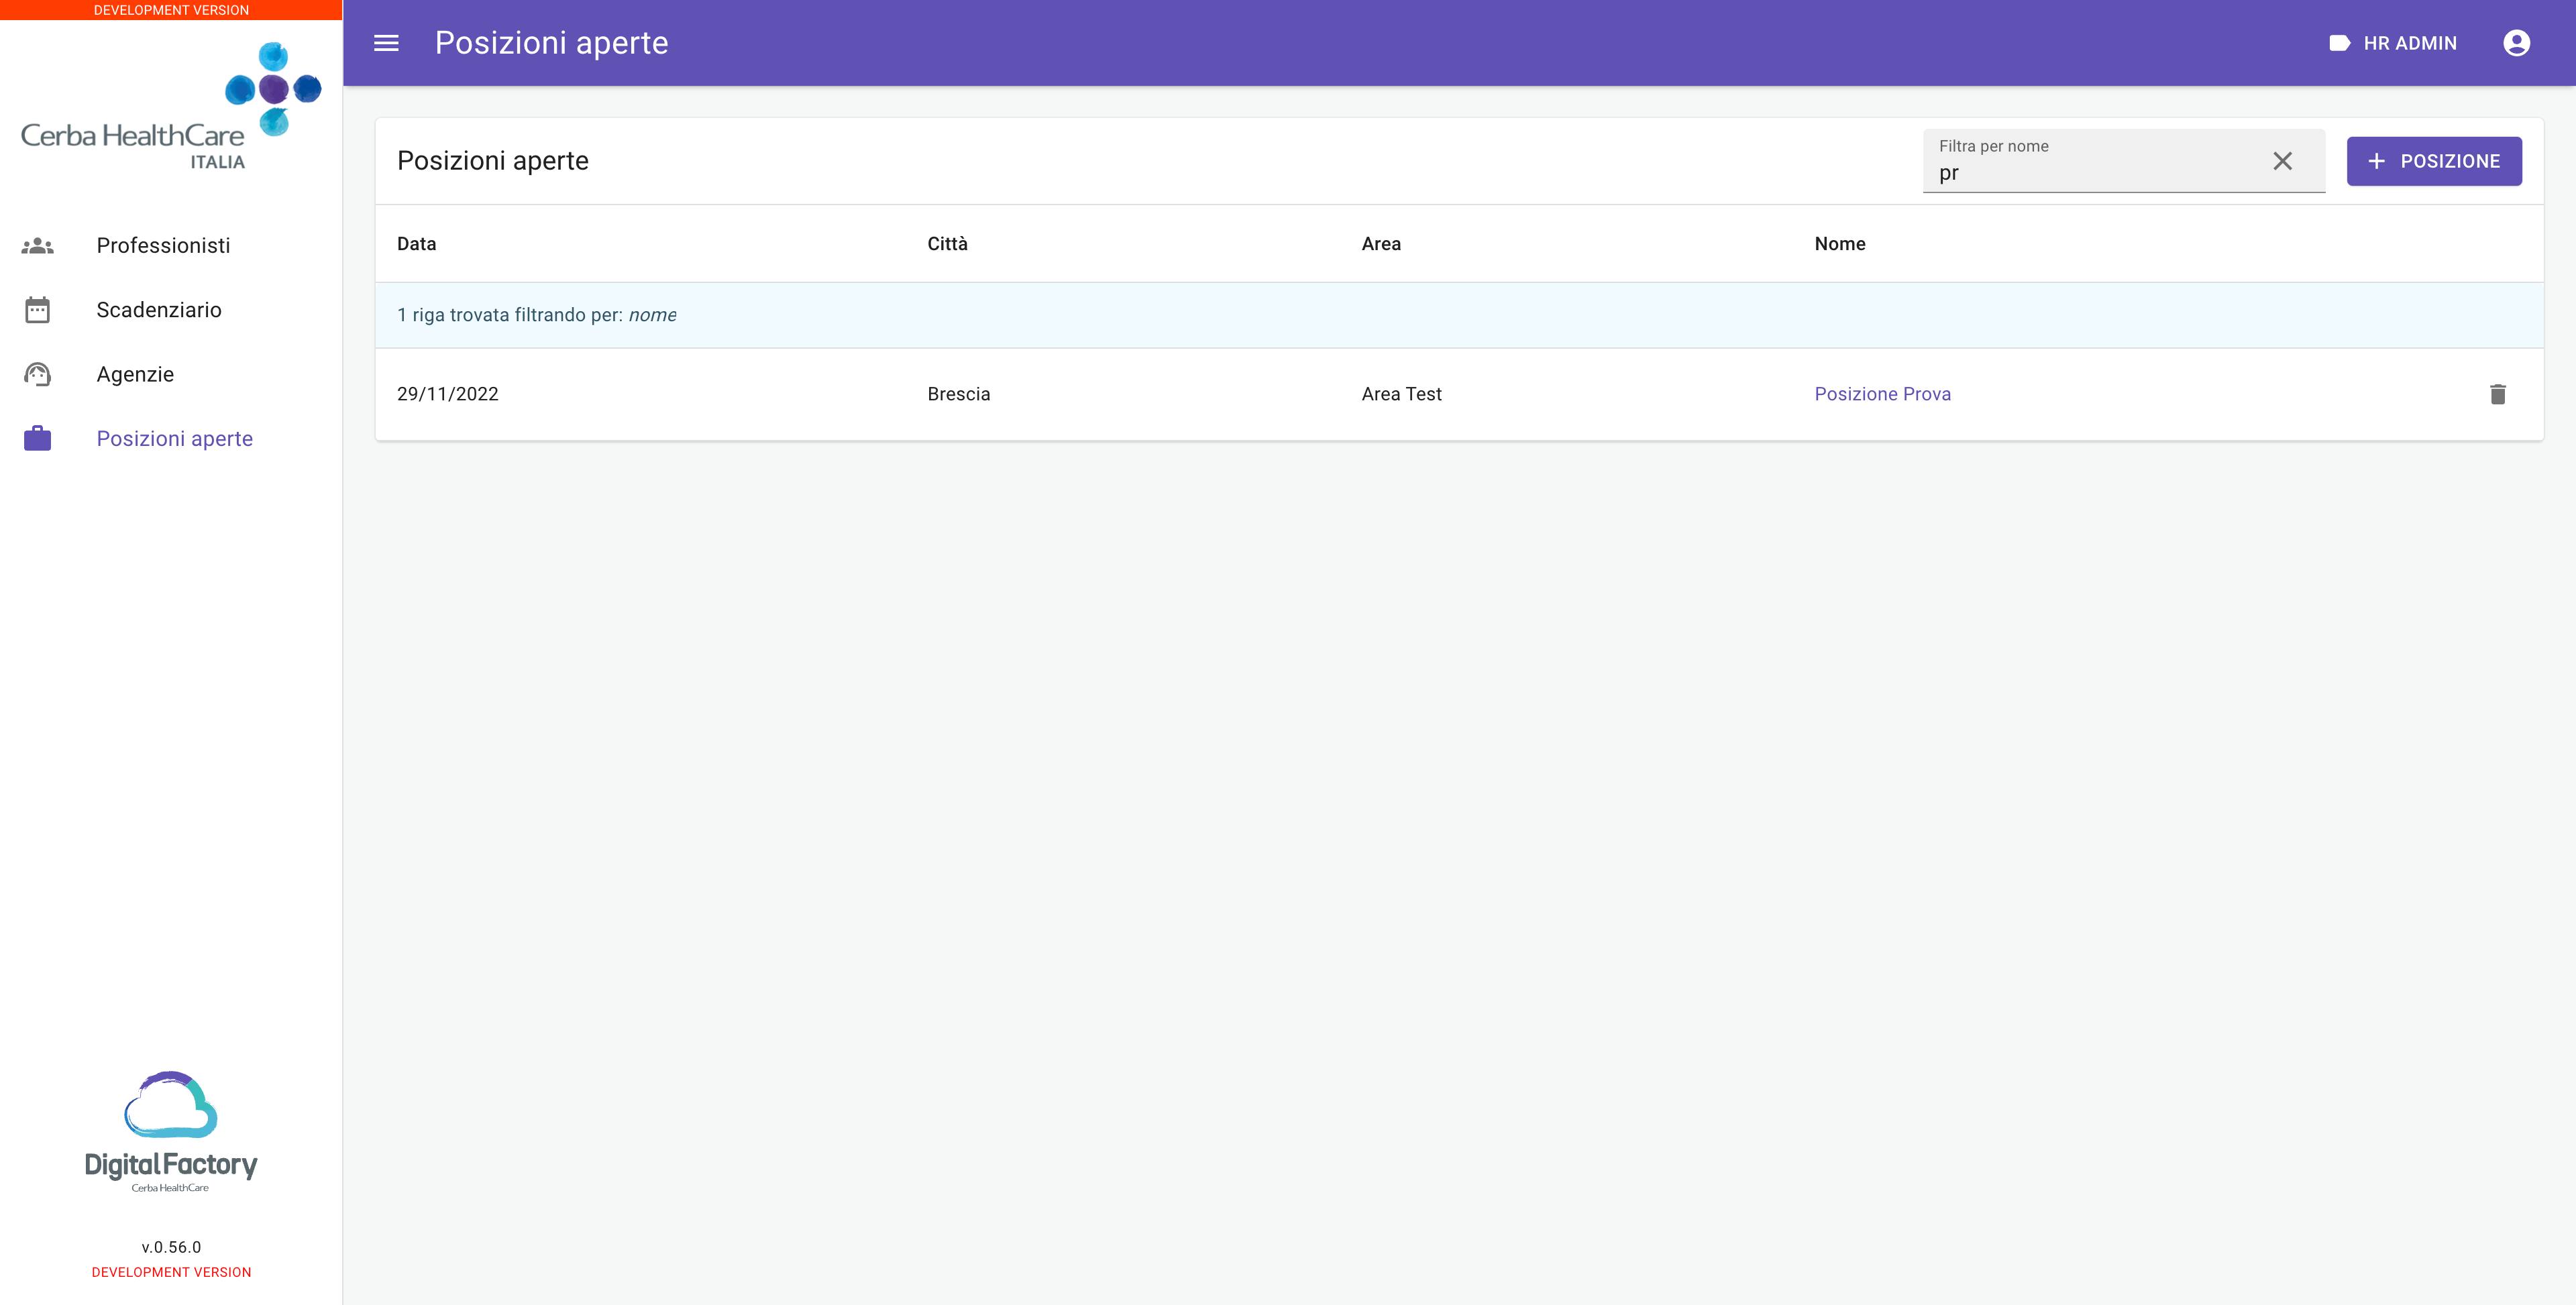
\includegraphics[width=0.75\textwidth]{images/capitolo5/f10_jobOpenPositions/PageJobOpenPositions_searchFilled.png} 
    \caption{Tabella posizioni aperte campo ricerca riempito} 
    \label{fig:PageJobOpenPositions_searchFilled}
\end{figure}

\begin{figure}[H]
    \centering
    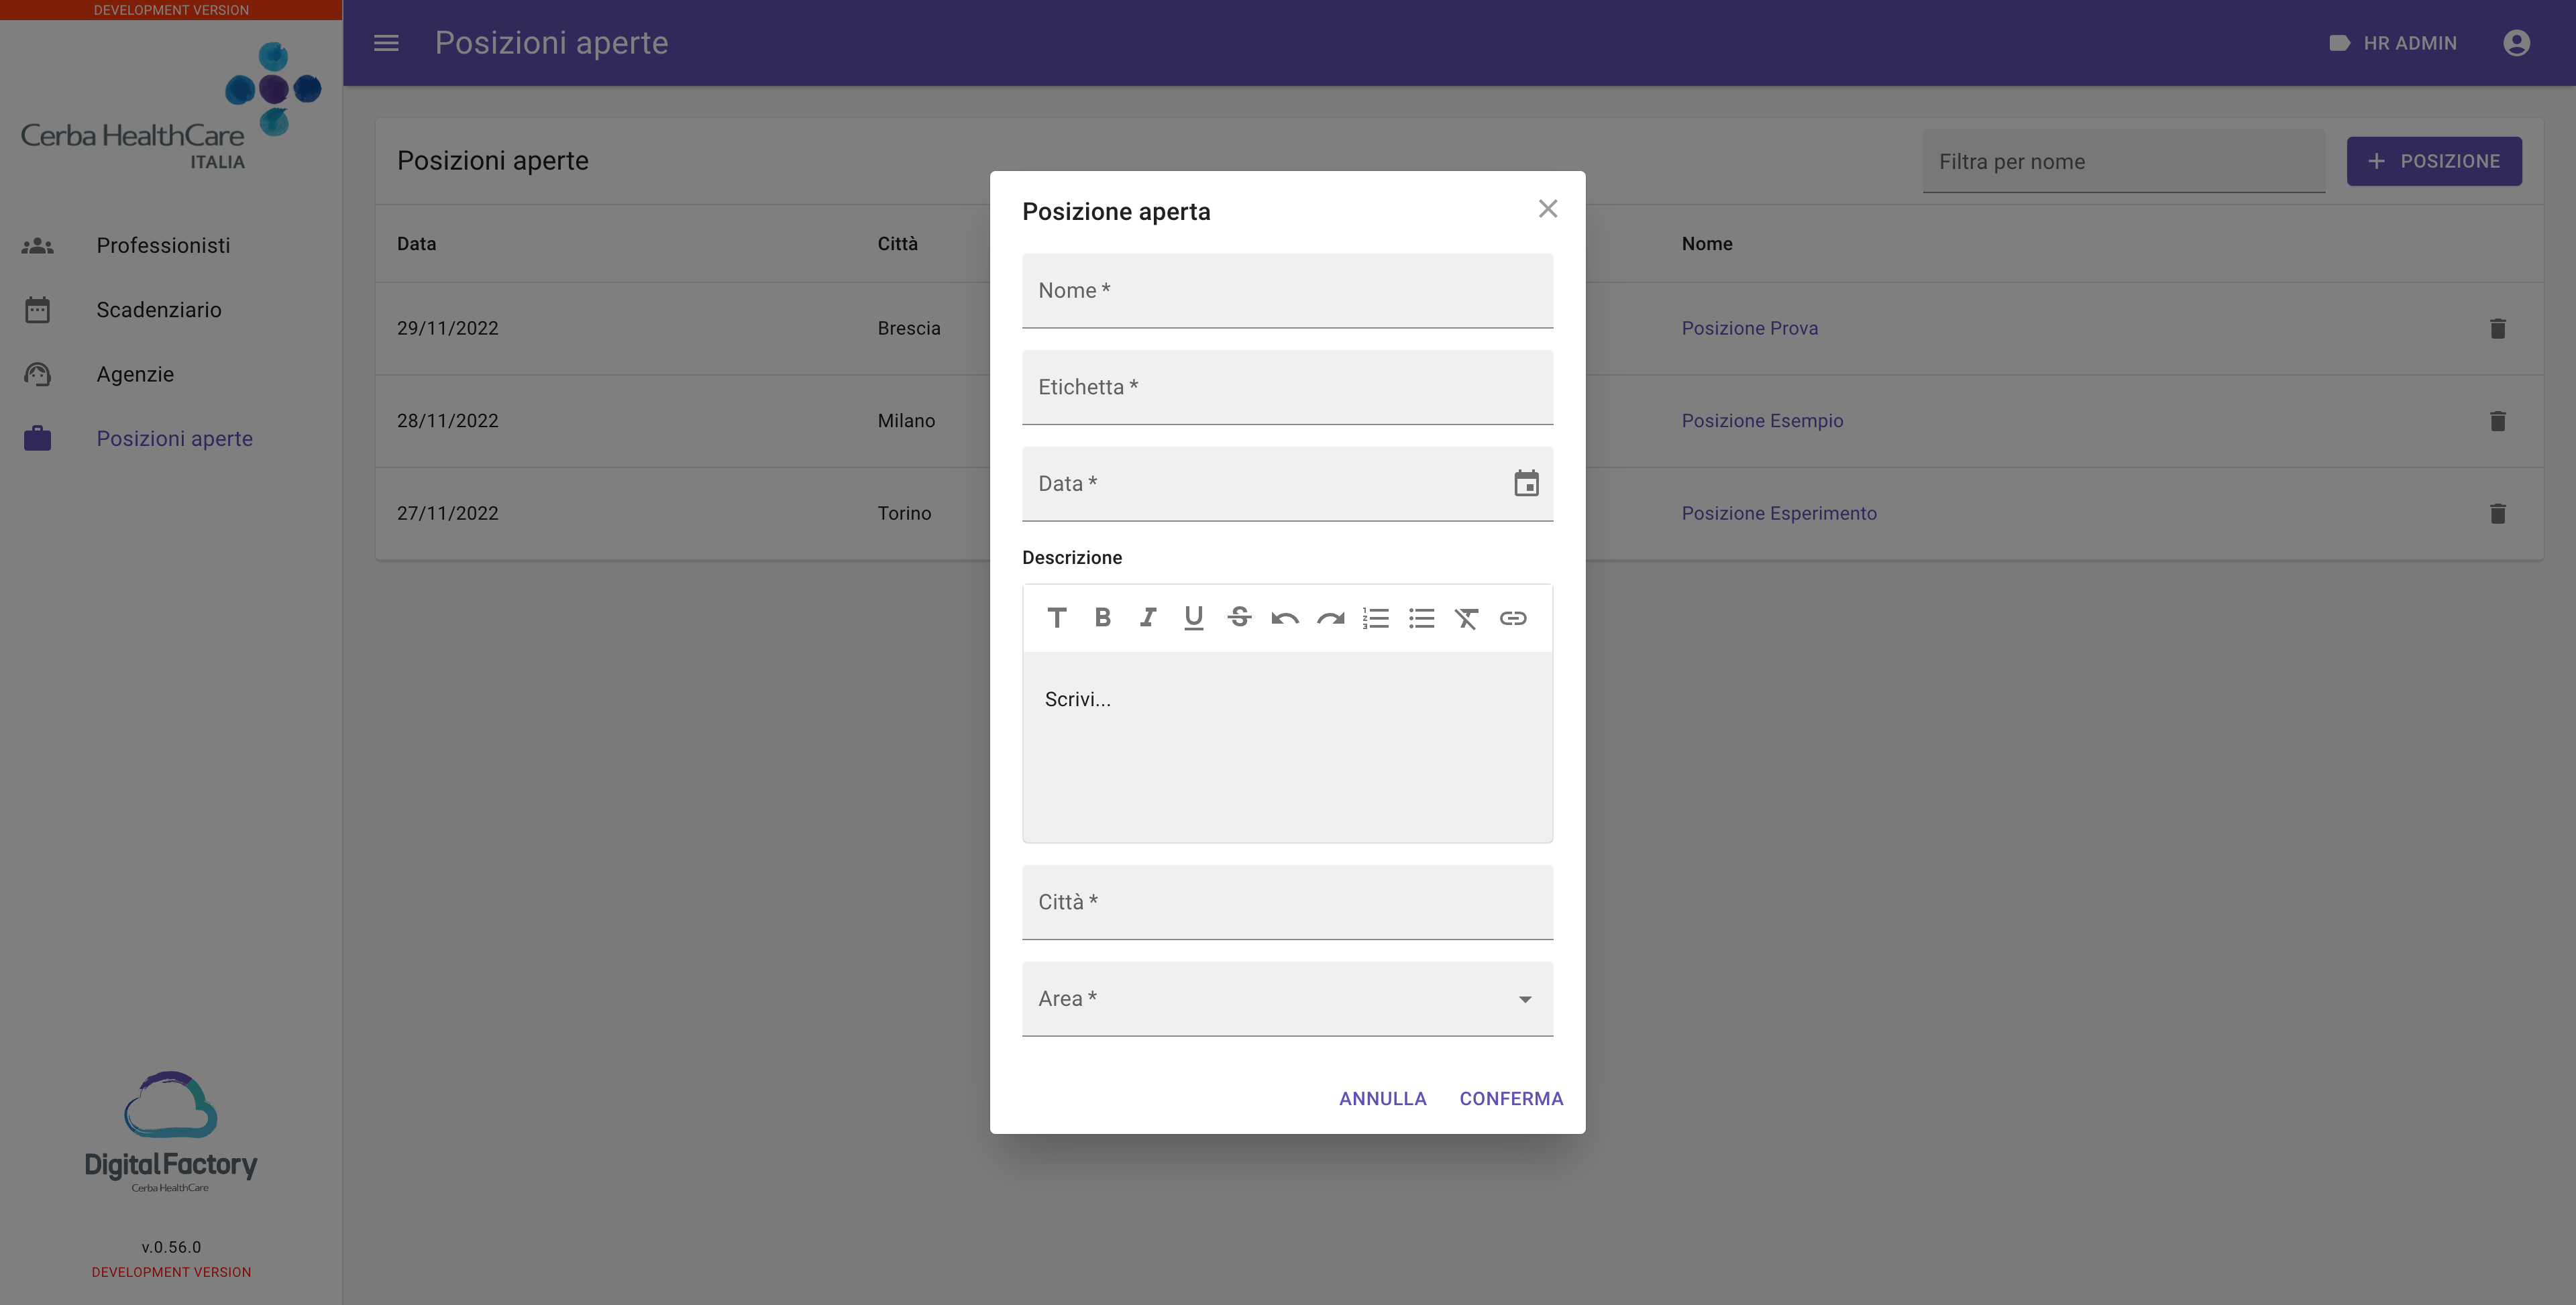
\includegraphics[width=0.75\textwidth]{images/capitolo5/f10_jobOpenPositions/ModalJobOpenPosition_create.png} 
    \caption{Modale aggiunta posizione aperta} 
    \label{fig:ModalJobOpenPosition_create}
\end{figure}

\begin{figure}[H]
    \centering
    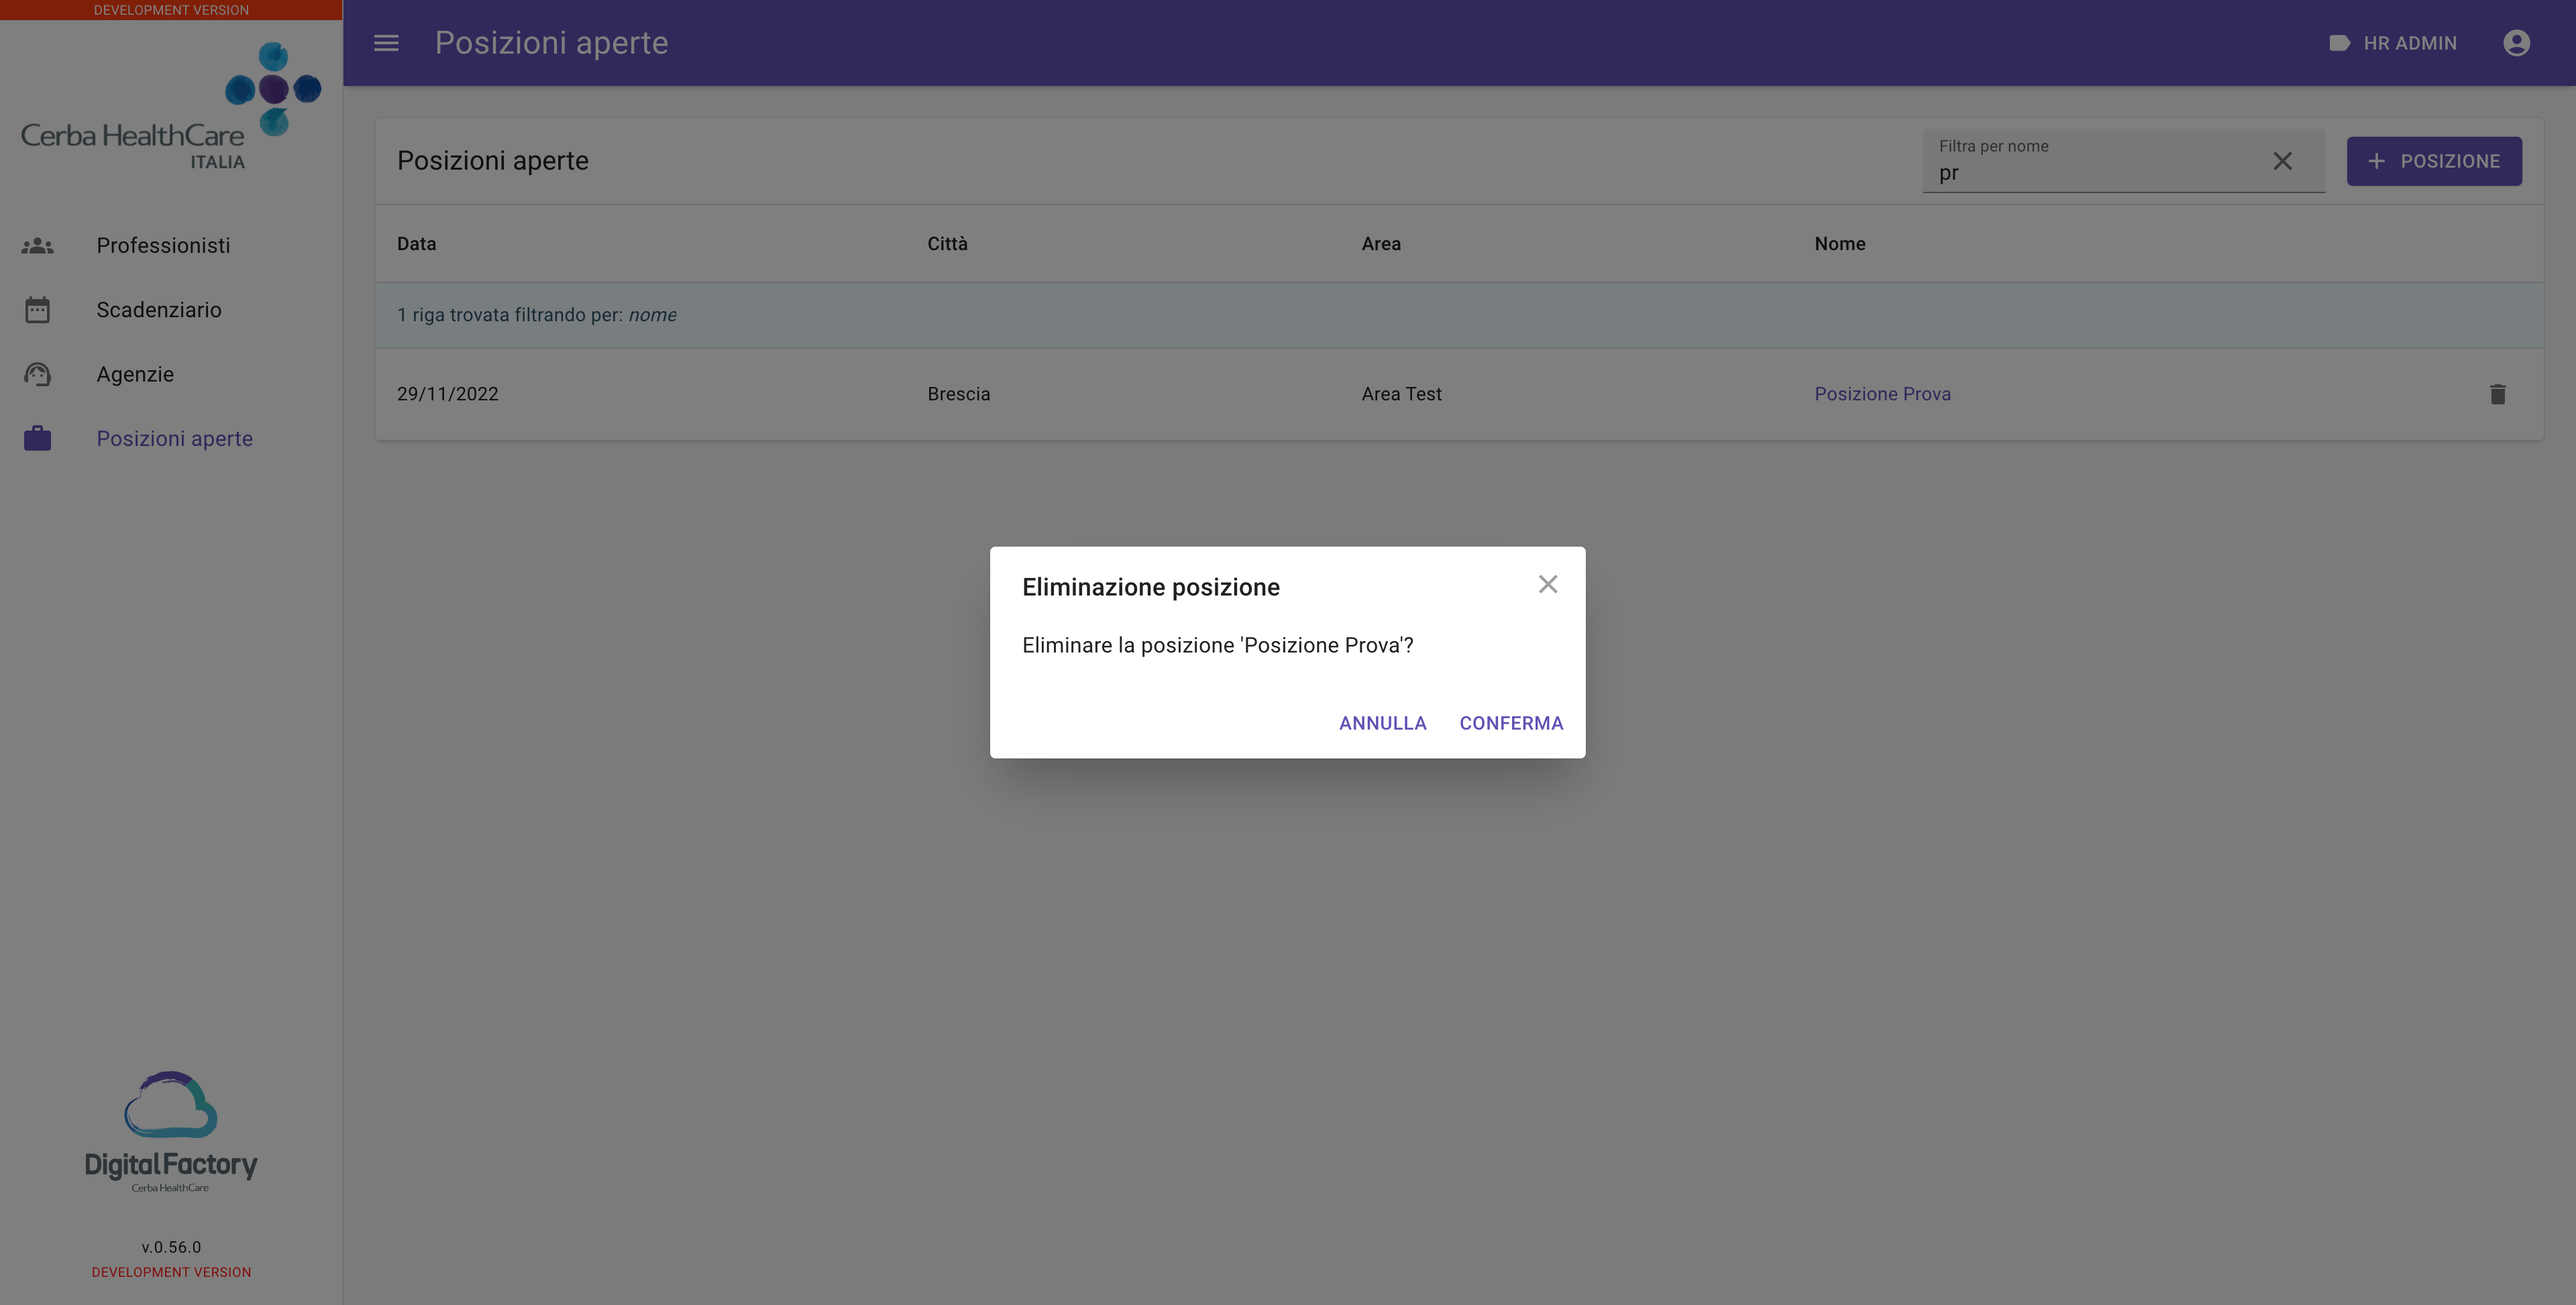
\includegraphics[width=0.75\textwidth]{images/capitolo5/f10_jobOpenPositions/ModalJobOpenPosition_delete.png} 
    \caption{Modale eliminazione posizione aperta} 
    \label{fig:ModalJobOpenPosition_delete}
\end{figure}

\begin{figure}[H]
    \centering
    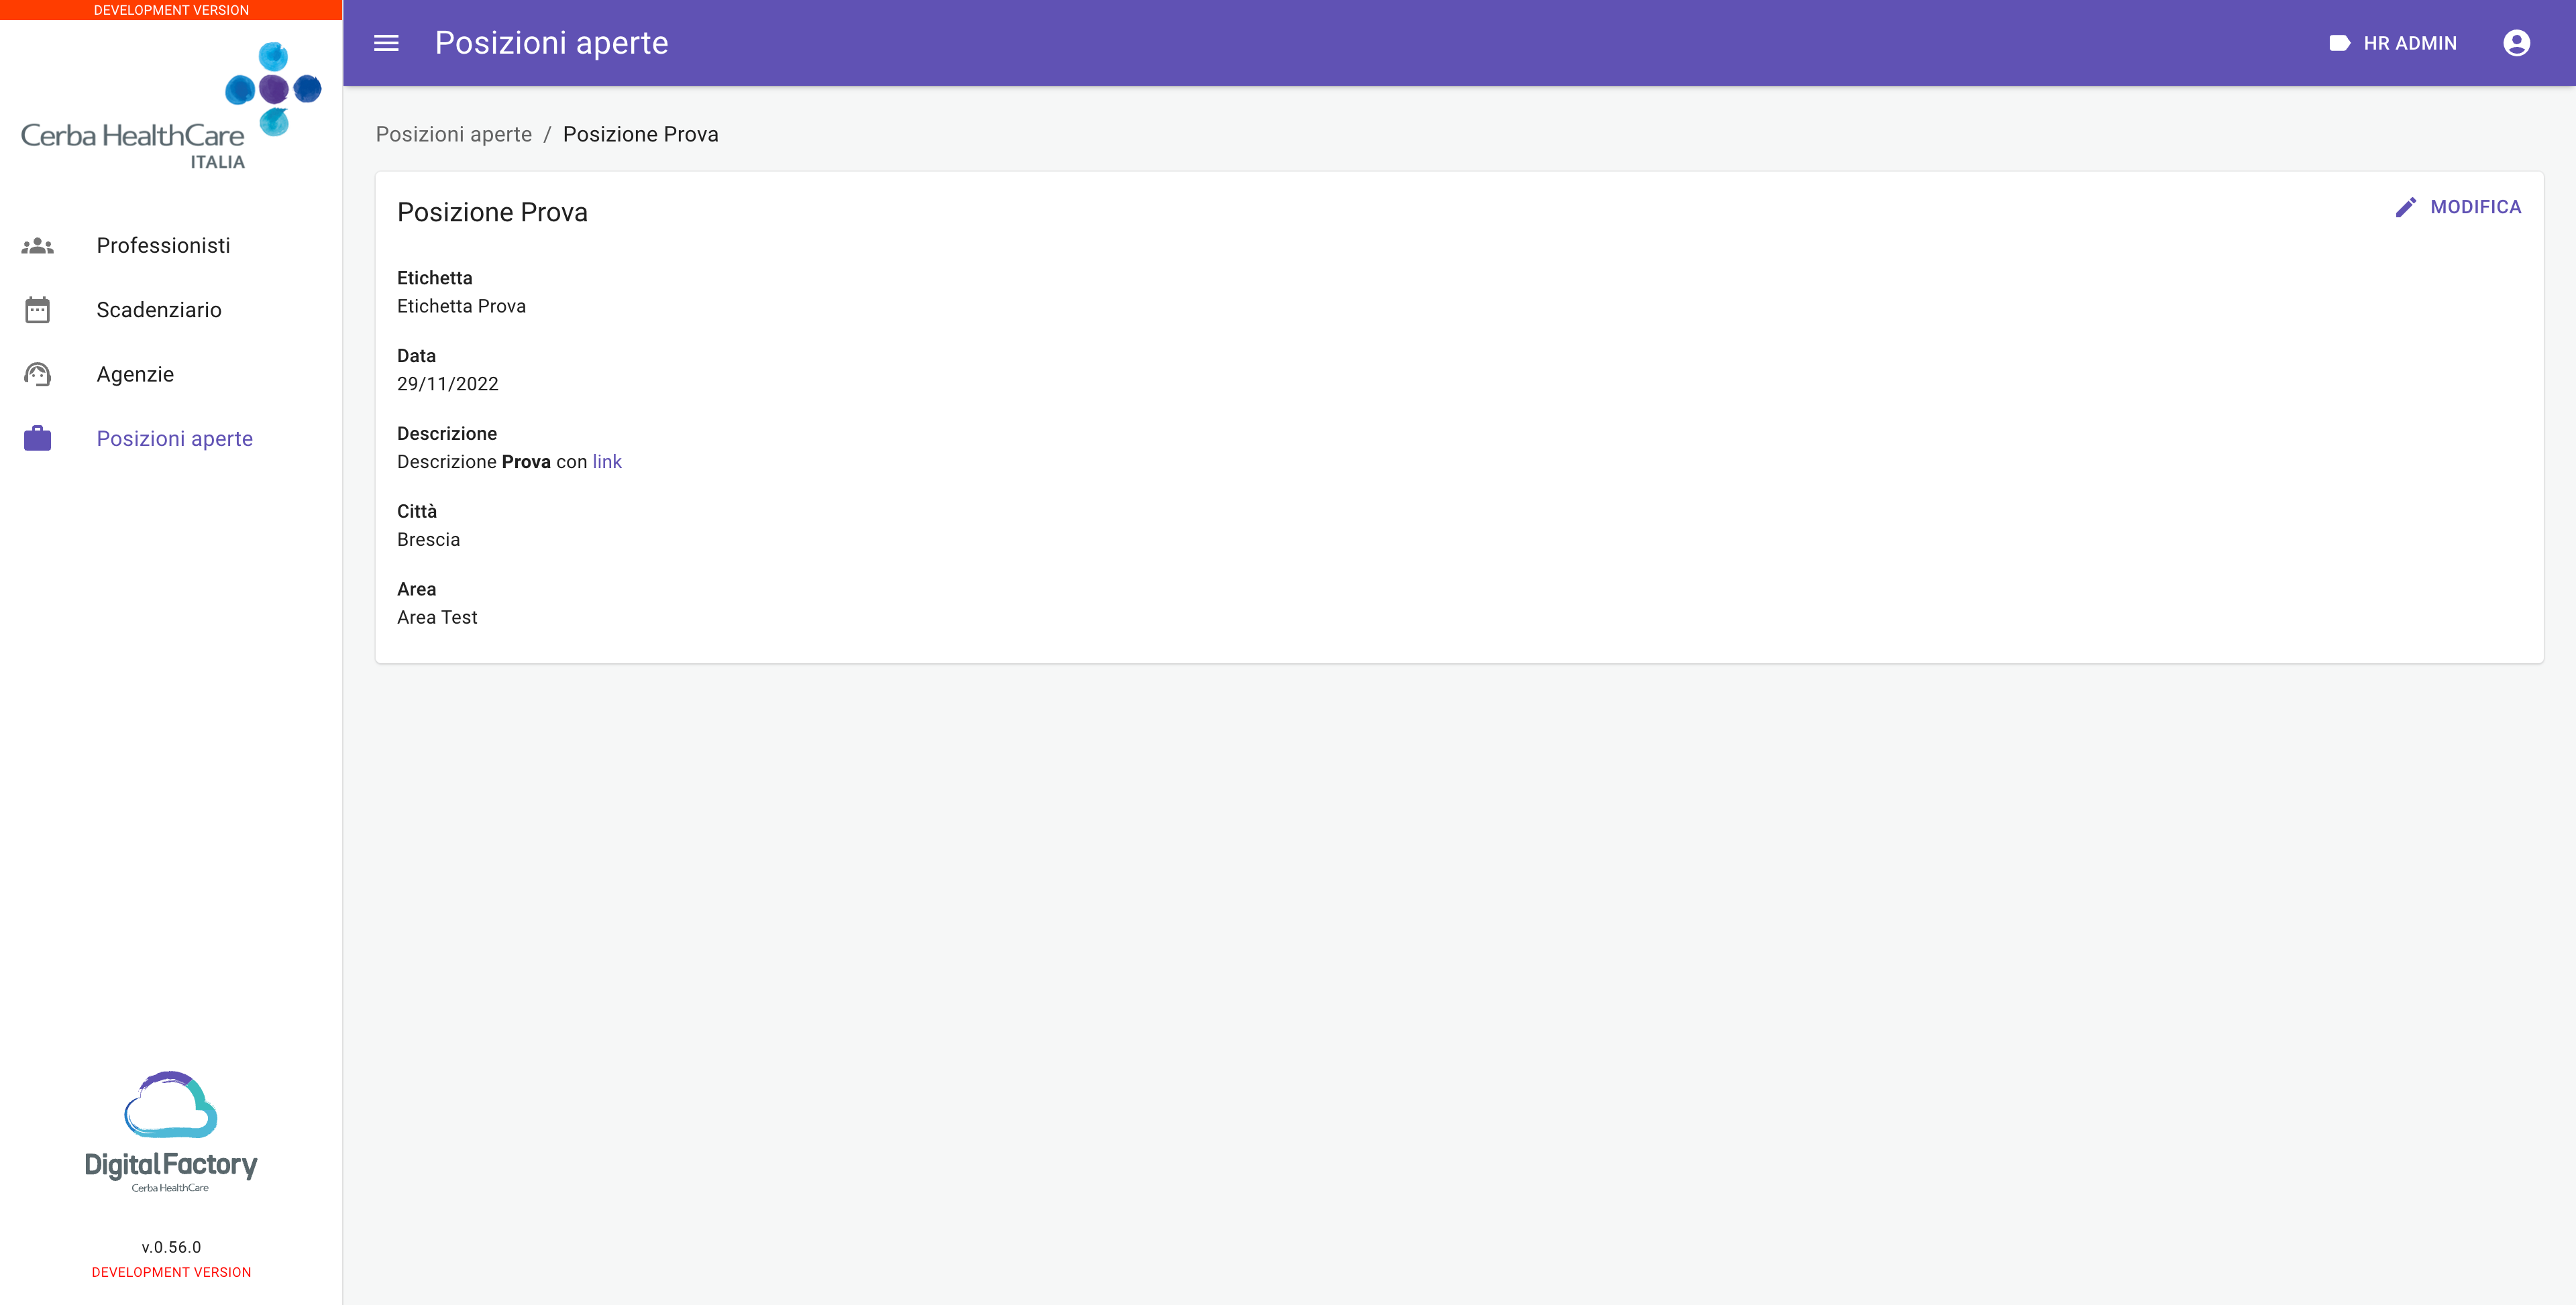
\includegraphics[width=0.75\textwidth]{images/capitolo5/f10_jobOpenPositions/PageJobOpenPosition.png} 
    \caption{Pagina dettaglio posizione aperta} 
    \label{fig:PageJobOpenPosition}
\end{figure}

\begin{figure}[H]
    \centering
    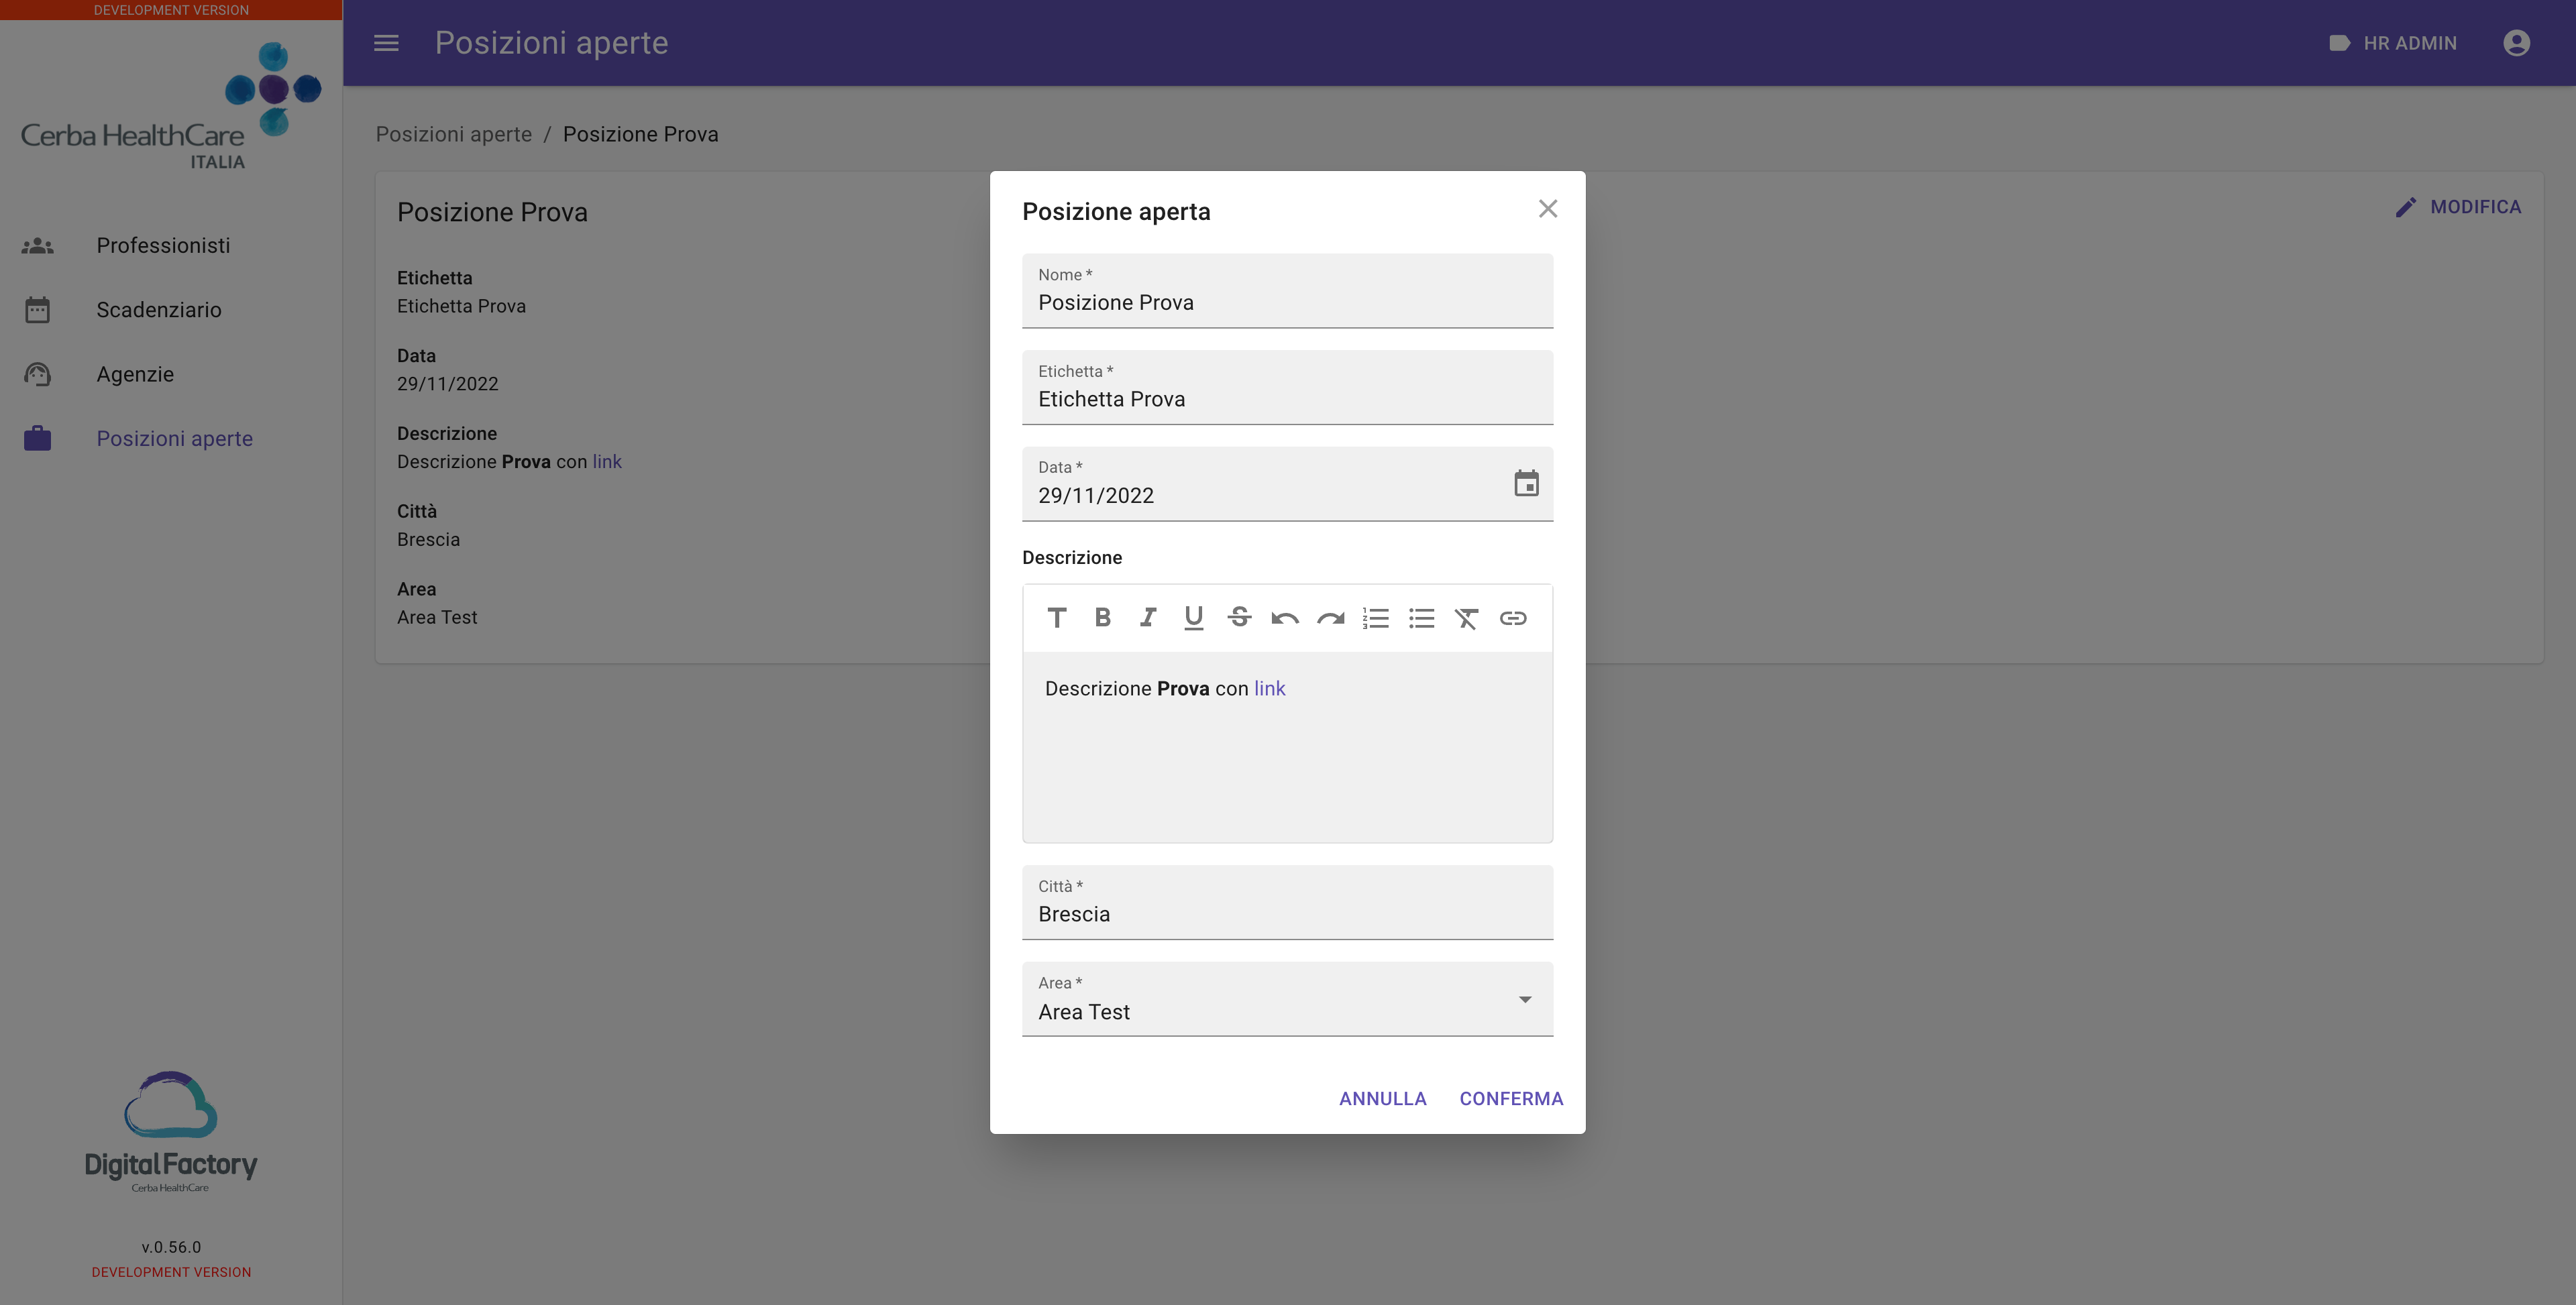
\includegraphics[width=0.75\textwidth]{images/capitolo5/f10_jobOpenPositions/ModalJobOpenPosition_edit.png} 
    \caption{Modale modifica posizione aperta} 
    \label{fig:ModalJobOpenPosition_edit}
\end{figure}

% \newpage\section{Bug}
% \label{sec:Bug}

% \subsection{B1: child}


\backmatter

\selectlanguage{italian}

\chapter{Conclusioni}
L'attività progettuale condotta ai fini dell'elaborato ha rappresentato un'esperienza di grande valore, che mi ha permesso di raggiungere diversi traguardi personali e di crescere professionalmente.

\textit{In primis}, ho potuto relazionarmi per la prima volta con il mondo del lavoro, nello specifico, interfacciandomi con una realtà disponibile e moderna come lo è Link-Up. Grazie all'inserimento in tale contesto aziendale, infatti, ho potuto sperimentare cosa significhi operare come sviluppatore \textit{front-end}, la figura professionale che ambisco a ricoprire in futuro, e far parte di un team interfunzionale in cui si collabora per far fronte a obiettivi comuni.\\
In secondo luogo, ho avuto l'opportunità di misurarmi con un progetto stimolante, collocato nell'innovativo e impattante contesto della Telemedicina. I vari mesi dedicati allo sviluppo delle implementazioni previste per il modulo “OMNIA”, di fatto, si sono tradotti da un lato in un applicativo aggiornato, che include le evolutive richieste dal committente, e che andrà a incidere positivamente sul flusso lavorativo di coloro che lo utilizzeranno quotidianamente, e dall'altro nell'oggetto protagonista della mia prova finale.

In aggiunta, nel corso dell'attività di sviluppo ho potuto accrescere le conoscenze in mio possesso attraverso i preziosi consigli ricevuti dai professionisti con i quali sono venuto a contatto, e applicare varie nozioni apprese tramite gli insegnamenti del corso di laurea.\\
Ancora una volta, va sottolineata l'importanza ricoperta delle librerie React e \acrlong*{mui}. Dato il fondamentale ruolo da esse ricoperto all'interno del progetto, con il loro impiego ho avuto l'opportunità di cimentarmi con due tecnologie estremamente al passo con i \textit{trend} attuali e di rilievo per gli sviluppatori \textit{front-end}. Il loro utilizzo ha suscitato in me il desidero di testare altre soluzioni che orbitano attorno al mondo di JavaScript e di React, nell'ottica di migliorare e accrescere l'attuale bagaglio di conoscenze. Ad ora, fra gli strumenti che più attirano il mio interesse vi sono React Native ed Electron, due \textit{framework} che permettono di sfruttare competenze di sviluppo web per la creazione di applicazioni \textit{mobile}. Ho avuto poi la possibilità di integrare all'interno della mia \textit{ruotine} lavorativa la metodologia agile di tipo \textit{Scrum}. Ciò mi ha consentito di familiarizzare con uno strumento largamente impiegato nell'ambito dello sviluppo del \textit{software}, e di rapportarmi con pregi e difetti di una strategia altamente dinamica, che, nel mio caso, ha previsto uno stretto contatto con il committente, con altri sviluppatori, e, alle volte, anche con il team di design.\\
Inoltre, ho potuto imbattermi in problemi e situazioni critiche caratteristiche di un'attività di sviluppo, nonché di un progetto così ambizioso. Infatti, è capitato di avere difficoltà nell'ambientarsi e nel destreggiarsi all'interno di un progetto già avviato, gestito da persone dotate di un maggior livello di competenza, nell'utilizzo di soluzioni tecnologiche che, in una certa misura, rappresentano una novità, oppure ancora nel dover adattare l'attività in svolgimento alle esigenze della prova finale. 

In conclusione, per quanto concerne il futuro dell'applicativo, il modulo “OMNIA” continuerà a essere gestito con le stesse modalità analizzate nel corso dell'elaborato. Per esso, seppur in misura minore rispetto al passato, sono programmate ulteriori evolutive che porteranno sia all'implementazione di nuove funzionalità per il supporto ad altri team, che alla loro ottimizzazione attraverso l'integrazione del \textit{feedback} ricevuto.\\
Invece, lo sviluppo della piattaforma per la digitalizzazione dei flussi di lavoro proseguirà perseguendo due obiettivi principali: per prima cosa, altri moduli che lo compongono, a rotazione (similmente a come è avvenuto per “OMNIA”), diverranno il fulcro dell'attività lavorativa del team per l'aggiunta di nuove funzioni; in secondo luogo, l'applicazione \textit{mobile}, esistente ma ancora in stato embrionale, verrà migliorata per avvicinarsi sempre di più all'essere uno strumento usabile e completo. 

\nocite{*}
\printbibliography[title=Bibliografia e Sitografia, heading=bibintoc]

% \printbibliography[keyword={site}, title=Sitografia, heading=bibintoc]
% \printbibliography[notkeyword={site}, heading=bibintoc]

\end{document}
% ----------------------------------------------------------